% Options for packages loaded elsewhere
\PassOptionsToPackage{unicode}{hyperref}
\PassOptionsToPackage{hyphens}{url}
%
\documentclass[
]{article}
\usepackage{amsmath,amssymb}
\usepackage{iftex}
\ifPDFTeX
  \usepackage[T1]{fontenc}
  \usepackage[utf8]{inputenc}
  \usepackage{textcomp} % provide euro and other symbols
\else % if luatex or xetex
  \usepackage{unicode-math} % this also loads fontspec
  \defaultfontfeatures{Scale=MatchLowercase}
  \defaultfontfeatures[\rmfamily]{Ligatures=TeX,Scale=1}
\fi
\usepackage{lmodern}
\ifPDFTeX\else
  % xetex/luatex font selection
\fi
% Use upquote if available, for straight quotes in verbatim environments
\IfFileExists{upquote.sty}{\usepackage{upquote}}{}
\IfFileExists{microtype.sty}{% use microtype if available
  \usepackage[]{microtype}
  \UseMicrotypeSet[protrusion]{basicmath} % disable protrusion for tt fonts
}{}
\makeatletter
\@ifundefined{KOMAClassName}{% if non-KOMA class
  \IfFileExists{parskip.sty}{%
    \usepackage{parskip}
  }{% else
    \setlength{\parindent}{0pt}
    \setlength{\parskip}{6pt plus 2pt minus 1pt}}
}{% if KOMA class
  \KOMAoptions{parskip=half}}
\makeatother
\usepackage{xcolor}
\usepackage{longtable,booktabs,array}
\usepackage{calc} % for calculating minipage widths
% Correct order of tables after \paragraph or \subparagraph
\usepackage{etoolbox}
\makeatletter
\patchcmd\longtable{\par}{\if@noskipsec\mbox{}\fi\par}{}{}
\makeatother
% Allow footnotes in longtable head/foot
\IfFileExists{footnotehyper.sty}{\usepackage{footnotehyper}}{\usepackage{footnote}}
\makesavenoteenv{longtable}
\usepackage{graphicx}
\makeatletter
\def\maxwidth{\ifdim\Gin@nat@width>\linewidth\linewidth\else\Gin@nat@width\fi}
\def\maxheight{\ifdim\Gin@nat@height>\textheight\textheight\else\Gin@nat@height\fi}
\makeatother
% Scale images if necessary, so that they will not overflow the page
% margins by default, and it is still possible to overwrite the defaults
% using explicit options in \includegraphics[width, height, ...]{}
\setkeys{Gin}{width=\maxwidth,height=\maxheight,keepaspectratio}
% Set default figure placement to htbp
\makeatletter
\def\fps@figure{htbp}
\makeatother
\ifLuaTeX
  \usepackage{luacolor}
  \usepackage[soul]{lua-ul}
\else
  \usepackage{soul}
\fi
\setlength{\emergencystretch}{3em} % prevent overfull lines
\providecommand{\tightlist}{%
  \setlength{\itemsep}{0pt}\setlength{\parskip}{0pt}}
\setcounter{secnumdepth}{-\maxdimen} % remove section numbering
% ============================================================================
% Custom preamble injected via `pandoc -H pandoc/preamble.tex`.
% This is added to whatever Pandoc generates, so all of the formatting below
% is re-applied automatically every time a new .docx is converted.
% ============================================================================

% --- Wider text block so figures and wide tables have room to breathe --------
\usepackage[letterpaper,margin=1in]{geometry}

% --- Never let a figure overflow the margins --------------------------------
% Caps images to the text area, preserving aspect ratio. postprocess.py also
% sizes images explicitly by type, but this is a belt-and-braces safety net.
\usepackage[export]{adjustbox}

% --- Attach whole external PDFs (Appendix J/I source documents) --------------
\usepackage{pdfpages}

% --- Landscape pages for very wide data tables (Appendix M) ------------------
\usepackage{pdflscape}

% --- Live table of contents titling ------------------------------------------
\renewcommand{\contentsname}{Table of Contents}

% --- Keep table titles/captions on the same page as their table --------------
\usepackage{needspace}

% --- Keep figures/tables and their captions on one page ----------------------
\usepackage{float}

% --- APA-7 URL/DOI line breaking ----------------------------------------------
% Pandoc's template loads xurl.sty, which allows a break at almost any
% character (including inside a DOI's digits, e.g. "10" / ".1145"). APA-7
% expects breaks at natural points instead — chiefly before a slash — so
% restrict \UrlBreaks to slash and hyphen, overriding xurl's aggressive set.
\makeatletter
\g@addto@macro\document{%
  \def\UrlBreaks{\do\/\do\-}%
}
\makeatother

% --- List of Figures / List of Tables titles ---------------------------------
\renewcommand{\listfigurename}{List of Figures}
\renewcommand{\listtablename}{List of Tables}

% --- Ease dense tables: smaller font + a little more row spacing -------------
% Applies to every longtable Pandoc emits. Extra-wide tables (6+ columns) are
% dropped a further step to \footnotesize by postprocess.py.
\usepackage{etoolbox}
% Row spacing is read from \longtablestretch so a single table can widen its
% rows (postprocess wraps text-heavy tables in a group that raises it) despite
% this hook running at every longtable's start.
\newcommand{\longtablestretch}{1.25}
\AtBeginEnvironment{longtable}{%
  \small
  \setlength{\tabcolsep}{5pt}%
  \renewcommand{\arraystretch}{\longtablestretch}%
}

% --- Let pdfLaTeX render Unicode math/Greek symbols found in the text --------
\ifPDFTeX
  \usepackage{newunicodechar}
  \newunicodechar{α}{\ensuremath{\alpha}}
  \newunicodechar{β}{\ensuremath{\beta}}
  \newunicodechar{γ}{\ensuremath{\gamma}}
  \newunicodechar{δ}{\ensuremath{\delta}}
  \newunicodechar{Δ}{\ensuremath{\Delta}}
  \newunicodechar{ε}{\ensuremath{\varepsilon}}
  \newunicodechar{η}{\ensuremath{\eta}}
  \newunicodechar{θ}{\ensuremath{\theta}}
  \newunicodechar{λ}{\ensuremath{\lambda}}
  \newunicodechar{μ}{\ensuremath{\mu}}
  \newunicodechar{π}{\ensuremath{\pi}}
  \newunicodechar{ρ}{\ensuremath{\rho}}
  \newunicodechar{σ}{\ensuremath{\sigma}}
  \newunicodechar{Σ}{\ensuremath{\Sigma}}
  \newunicodechar{τ}{\ensuremath{\tau}}
  \newunicodechar{φ}{\ensuremath{\varphi}}
  \newunicodechar{χ}{\ensuremath{\chi}}
  \newunicodechar{ψ}{\ensuremath{\psi}}
  \newunicodechar{ω}{\ensuremath{\omega}}
  \newunicodechar{Ω}{\ensuremath{\Omega}}
  \newunicodechar{×}{\ensuremath{\times}}
  \newunicodechar{÷}{\ensuremath{\div}}
  \newunicodechar{±}{\ensuremath{\pm}}
  \newunicodechar{∓}{\ensuremath{\mp}}
  \newunicodechar{≤}{\ensuremath{\leq}}
  \newunicodechar{≥}{\ensuremath{\geq}}
  \newunicodechar{≠}{\ensuremath{\neq}}
  \newunicodechar{≈}{\ensuremath{\approx}}
  \newunicodechar{−}{\ensuremath{-}}
  \newunicodechar{→}{\ensuremath{\rightarrow}}
  \newunicodechar{∞}{\ensuremath{\infty}}
  \newunicodechar{∑}{\ensuremath{\sum}}
  \newunicodechar{√}{\ensuremath{\surd}}
  \newunicodechar{☐}{\ensuremath{\square}}
  \newunicodechar{☒}{\ensuremath{\boxtimes}}
\fi
\ifLuaTeX
  \usepackage{selnolig}  % disable illegal ligatures
\fi
\IfFileExists{bookmark.sty}{\usepackage{bookmark}}{\usepackage{hyperref}}
\IfFileExists{xurl.sty}{\usepackage{xurl}}{} % add URL line breaks if available
\urlstyle{same}
\hypersetup{
  hidelinks,
  pdfcreator={LaTeX via pandoc}}

\author{}
\date{}

\begin{document}
\begin{titlepage}
\centering
\vspace*{\fill}


\includegraphics[width=0.32\linewidth]{media/media/image37.png}

\vspace{0.8cm}

Hochschule Rhein-Waal

Rhine-Waal University of Applied Sciences

Faculty of Communication and Environment

Prof. Dr. Kai Essig

André Frank Krause

\vspace{1.6cm}

{\Large\bfseries Designing and Evaluating Usability-Centred Onboarding and Calibration Workflows in Multi-Modal Research Platforms\par}

\vspace{1.6cm}

Master Thesis

Submitted to the Degree of Master of Science

in

Usability Engineering

\vspace{0.8cm}

by Daniyal Admany

Matriculation number: 35795

Submission Date: 15.07.2026

\vspace*{\fill}
\end{titlepage}

\pagenumbering{roman}
\setcounter{tocdepth}{4}
\clearpage
\hypertarget{acknowledgements}{%
\section{Acknowledgements}\label{acknowledgements}}

I would like to thank my supervisor, Prof. Dr. Kai Essig, whose guidance and feedback shaped this work at every stage and consistently pushed it to be clearer and more rigorous than I would have managed alone. And to my second supervisor, Dr. André Frank Krause, for his time and considered input.

Big thanks to Sarthak and Shilton, without whose efforts, the Sensa prototype would not have been built. Running from the campus to the bus stop to catch the last SB30 back to Duisburg has been a core part of my experience during this programme, and it was apt that the last few months reflected that. And to Renu for her help, snacks, and company in the lab. And of course to the twelve participants, whose patience and honesty made this study possible.

To my family, thank you for everything. To my mother especially, who always wanted me to do a Master\textquotesingle s: this one is for you. And to my friends, thank you for always (trying to) keeping me grounded.

\clearpage
\hypertarget{abstract}{%
\section{Abstract}\label{abstract}}

Multi-sensor research platforms combine eye tracking with physiological sensors such as electrodermal activity, but setting up and calibrating these instruments is typically done through several disconnected tools, each with its own interface and procedure. This fragmentation creates avoidable friction during onboarding and calibration, yet the usability of the setup process itself is rarely evaluated. This thesis designed a unified, guided onboarding and calibration workflow within the Sensa platform and evaluated it against a fragmented multi-tool baseline. The central question was whether integrating the setup into a single guided flow improves usability without degrading the quality of the eye-tracking calibration it produces.

A within-subjects, counterbalanced study was conducted with twelve participants, each completing both workflows. Efficiency, perceived workload, perceived usability, and observed interaction breakdowns were measured alongside eye-tracking calibration quality, which was treated as a validity safeguard rather than a performance target. Written participant responses and observation notes were analysed using reflexive thematic analysis.

The unified workflow substantially reduced perceived workload and interaction breakdowns and raised perceived usability from below to above the established benchmark, all with large effects. Setup and calibration times were shorter but did not reach the corrected significance threshold. Calibration quality showed no significant differences in gaze accuracy, valid data yield, or first-pass success, while gaze precision was poorer in the unified condition, concentrated in two low-yield sessions. The qualitative findings indicate that visible system state reduced the uncertainty driving breakdowns in fragmented setups. The study shows that guided integration can improve setup usability without detectable loss of calibration quality.

\textbf{Keywords}: usability engineering; multi-sensor research platforms; eye-tracking validation; biosensor setup; eda baseline; guided onboarding workflows; reflexive thematic analysis; interaction breakdowns; within-subjects evaluation

\clearpage
\tableofcontents
\clearpage

\clearpage
\hypertarget{list-of-abbreviations}{%
\section{List of Abbreviations}\label{list-of-abbreviations}}

\begin{longtable}[]{@{}p{0.18\columnwidth}p{0.75\columnwidth}@{}}
AI & Artificial Intelligence \\
APA & American Psychological Association \\
CI & Confidence Interval \\
ECG & Electrocardiography \\
EDA & Electrodermal Activity \\
EEG & Electroencephalography \\
GSR & Galvanic Skin Response \\
HCI & Human--Computer Interaction \\
HR & Heart Rate \\
HRV & Heart Rate Variability \\
HSRW & Rhine-Waal University of Applied Sciences (Hochschule Rhein-Waal) \\
JASP & Jeffreys's Amazing Statistics Program (statistical software) \\
M & Mean \\
NASA-TLX & NASA Task Load Index \\
OBS & Open Broadcaster Software \\
RMSSD & Root Mean Square of Successive Differences \\
SD & Standard Deviation \\
SUS & System Usability Scale \\
UI & User Interface \\
UX & User Experience \\
\end{longtable}


\clearpage
\hypertarget{list-of-figures-list-of-tables}{}%
\phantomsection\addcontentsline{toc}{section}{List of Figures}
\listoffigures
\phantomsection\addcontentsline{toc}{section}{List of Tables}
\listoftables




\clearpage
\pagenumbering{arabic}
\clearpage
\hypertarget{introduction}{%
\section{1. Introduction}\label{introduction}}

\hypertarget{background-and-motivation}{%
\subsection{1.1 Background and Motivation}\label{background-and-motivation}}

The use of biometric sensors in multimodal research platforms is rapidly increasing, especially in systems that combine eye tracking with sensors such as electroencephalography (EEG). These platforms are increasingly used in Human-Computer Interaction (HCI) and usability engineering research (Zhu \& Lv, 2023, p. 2). Gaspar-Figueiredo et al. (2026, pp. 1-3) argue that multimodal sensor systems can record behavioural and physiological signals, such as gaze behaviour and EEG activity. Their main advantage over traditional self-report methods is that they provide objective, real-time insights into users\textquotesingle{} cognitive workload and emotional responses, while surveys and interviews mainly capture subjective user perceptions,which participants can only report consciously. By recording objective, measurable data, multimodal setups have become important for studies in fields including automotive HMI, UX research, and adaptive interface design (Aloi et al., 2024, p. 1; Gaspar-Figueiredo et al., 2026, p. 1).

Despite their analytical value, multi-sensor research platforms remain complex to prepare and operate. While calibration, onboarding, session recording, and data analysis are all integral components of multi-sensor research platforms, prior work (Aloi et al., 2024; Zhu \& Lv, 2023) identifies onboarding and calibration as the stage most prone to usability breakdowns and requiring repeated iterations, high cognitive effort, and technical expertise. These difficulties are not only UX challenges (for example unclear system status, no feedback on whether a step has succeeded, and no guidance on the next required action) but concrete technical-procedural ones: users must correctly place sensors, configure them according to study requirements, ensure proper sensor contact by attaching gelled snap electrodes to the skin, check signal quality, and repeat calibration steps when the recorded data are unreliable.

Each of these steps is technically critical, since poor execution affects not only setup efficiency but also the validity of the recorded data (Aloi et al., 2024; Zhu \& Lv, 2023; Drewes et al., 2019). This thesis therefore isolates onboarding and calibration as its primary research focus, and investigates how a web-based multi-sensor research platform with a unified, usability-centred onboarding and calibration flow (a single guided sequence that walks the researcher through sensor selection, placement, signal-quality checks, calibration, and validation, with continuous feedback on system status) can reduce setup and calibration time, decrease cognitive workload for the user, and improve perceived usability.

While prior research has emphasized the analytical benefits of combining eye-tracking and physiological sensors, and has acknowledged that calibration and onboarding in multi-sensor environments are time-consuming and complex, few studies have systematically evaluated how intuitive, efficient, and error-prone the setup and calibration process is for users before the actual measurement begins. Existing work primarily focuses on signal accuracy, synchronization techniques, or methodological validity rather than on how workflow structure and interaction design influence user performance during setup. A more detailed review of the relevant literature is presented in Chapter 2.

This thesis contributes empirical evidence by experimentally comparing a traditional, fragmented workflow (in which each sensor is set up and calibrated separately, typically across two or more disconnected tools) with a unified, software-guided workflow, under controlled conditions; specifically the task, sensor setup, environment, instructions, timing, and calibration procedure. Beyond measuring efficiency and workload, it analyses observable interaction breakdowns and operationalizes calibration outcome quality using measurable indicators such as accuracy, reliability, and successful completion. In doing so, the thesis addresses both workflow usability and technical calibration quality, with the former as the primary research target and the latter as a validity safeguard, providing actionable insights for the design of human-centred multi-sensor research platforms.

\hypertarget{problem-statement}{%
\subsection{\texorpdfstring{1.2 Problem Statement }{1.2 Problem Statement }}\label{problem-statement}}

The specific problem this thesis addresses is that the technically critical setup steps described in Chapter 1.1 must typically be performed across two or more disconnected tools. When the workflow does not support these steps sufficiently, the result can be high cognitive workload, repeated setup errors, longer setup times, unreliable calibration, and potentially invalid data.

In practice, this fragmentation manifests as a sequential multi-tool workflow: researchers must first position themselves and calibrate an eye tracker using the manufacturer\textquotesingle s own eye-tracking software (for example, Tobii Core), before separately placing biosensor electrodes, establishing a Bluetooth device connection, and verifying signal integrity by visual inspection of live waveforms in a second tool such as OpenSignals. Each tool operates independently, with no shared state, no cross-system readiness feedback, and no unified error handling. This not only increases total setup time but also creates several potential failure points, including calibration failure and tracking degradation, that require researchers to monitor data quality and understand the limitations of each system (Van Lier et al., 2020; Cuve et al., 2022).

As noted by Aloi et al. (2024) and Zhu and Lv (2023), such barriers limit adoption, especially among novice researchers or small teams. While prior work has examined the analytical value of multi-modal data, there is a lack of systematic evaluation of how onboarding and calibration workflow design affects both usability and the technical correctness of the calibration result.

This highlights the need for a \textbf{unified, user-centred workflow} that integrates the setup, calibration, and synchronization of all sensors into a single, streamlined process. In a unified workflow, eye-tracking and biometric sensors are configured and calibrated together, reducing redundant steps, minimizing manual coordination, and improving both efficiency and confidence in the quality of the collected multi-modal data.

\hypertarget{research-aim}{%
\subsection{1.3 Research Aim}\label{research-aim}}

This thesis aims to build and empirically evaluate an integrated usability-centred onboarding and calibration workflow for multi-sensor research environments, and to compare it against a fragmented workflow using separate tools per modality. The evaluation covers five outcome dimensions: setup efficiency, cognitive workload, perceived usability, interaction breakdowns, and calibration outcome quality. In doing so, the aim is to address both workflow usability and the technical requirements of correct sensor setup and reliable calibration, with workflow usability as the primary research target and calibration quality as a validity safeguard that ensures any usability gains do not come at the cost of data quality.

To address this, a unified, usability-centred onboarding and calibration workflow, as part of a broader platform (hereon referred to as \emph{\textbf{Sensa}}), was designed and implemented within a functional prototype developed in the Usability Lab at Rhine-Waal University. The prototype provided guided sensor selection, step-by-step sensor placement instructions, device configuration support, signal-quality checks, eye-tracking calibration guidance, eye-tracking validation, readiness checks before recording, and corrective feedback. The readiness check confirms that the participant is seated correctly, that lighting is adequate, that all sensors are visible and accessible, and that gelled snap electrodes are attached before recording begins; corrective feedback provides in-context prompts that identify what is wrong and how to fix it when a step fails.

The prototype was then empirically evaluated against an existing fragmented workflow using objective performance measures (setup time, calibration time, and observed interaction breakdowns), subjective measures (NASA-TLX and SUS), and calibration quality indicators (eye-tracking gaze accuracy, gaze precision, valid data yield, and first-pass calibration success). All of these measures were collected in both the unified and the fragmented condition, since the study used a within-subjects design in which each participant completed both workflows.

In addition to comparing overall task time, this study seeks to identify and categorize the concrete interaction breakdowns that cause delays and higher workload in fragmented workflows. Examples include repeated setup steps, unclear feedback, hesitation, uncertainty about device synchronization, difficulty interpreting signal-quality indicators, and confusion about the next required action. This analysis matters because total task time alone does not reveal why one workflow is less efficient than another; identifying the specific points at which fragmented workflows break down provides actionable design insight for future multi-sensor research platforms.

The empirical evaluation focuses specifically on the onboarding and calibration workflow contributed by the author within Sensa; the precise nature and boundaries of that contribution are set out in Chapter 3.3.

\hypertarget{research-questions}{%
\subsection{\texorpdfstring{1.4 Research Questions }{1.4 Research Questions }}\label{research-questions}}

This thesis investigates how workflow structure and guided interaction design influence efficiency, usability, and calibration outcomes in multi-sensor research environments. The five outcome dimensions identified in the Research Aim (Chapter 1.3) are reflected in the following research questions, which guide the empirical study:

\begin{enumerate}
\def\labelenumi{\arabic{enumi}.}
\item
  Which workflow steps and interaction breakdowns contribute most to time consumption during onboarding and calibration in fragmented multi-sensor setups?
\item
  Does a unified, software-guided onboarding and calibration workflow reduce total setup and calibration time compared to a fragmented multi-tool workflow?
\item
  How does a unified software-guided onboarding and calibration workflow affect perceived workload, usability, and user confidence in the calibration process?
\item
  How does a unified, software-guided onboarding and calibration workflow affect calibration outcome quality compared to a fragmented multi-tool workflow, as measured by gaze accuracy, gaze precision, valid data yield, and first-pass calibration success?
\end{enumerate}

\hypertarget{hypotheses}{%
\subsection{1.5 Hypotheses}\label{hypotheses}}

Based on prior literature and the proposed unified workflow design, the following hypotheses are formulated:

\begin{itemize}
\item
  \textbf{H1}: Participants will complete setup and calibration significantly faster in the unified workflow condition than in the fragmented workflow.

  \begin{itemize}
  \item
  Setup time and calibration time are measured and analysed as two separate variables, each operationalised in Chapter 4.5.1.
  \end{itemize}
\item
  \textbf{H2}: Participants will report significantly lower perceived workload (NASA-TLX) in the unified workflow than in the fragmented workflow
\item
  \textbf{H3}: Participants will report significantly higher perceived usability (SUS) in the unified workflow than in the fragmented workflow.
\item
  \textbf{H4:} Participants will exhibit fewer observable interaction breakdowns (e.g., step repetition, hesitation, incorrect sequence execution) in the unified workflow than in the fragmented workflow

  \begin{itemize}
  \item
  The categories of observable breakdown and their coding criteria are defined in Chapter 4.5.3.
  \end{itemize}
\item
  \textbf{H5:} The unified workflow will achieve eye-tracking calibration quality comparable to the fragmented workflow across (a) gaze accuracy, (b) gaze precision, and (c) valid data yield, with (d) first-pass calibration success no lower than in the fragmented workflow.

  \begin{itemize}
  \item
  See Chapter 4.5.4 for operationalization.
  \end{itemize}
\end{itemize}

\Needspace{13\baselineskip}
Each hypothesis maps directly onto one of the research questions in Chapter 1.4, with each addressing a specific outcome dimension identified in the Research Aim:

\begin{longtable}[]{@{}
  >{\raggedright\arraybackslash}p{(\columnwidth - 4\tabcolsep) * \real{0.0907}}
  >{\raggedright\arraybackslash}p{(\columnwidth - 4\tabcolsep) * \real{0.7804}}
  >{\raggedright\arraybackslash}p{(\columnwidth - 4\tabcolsep) * \real{0.1089}}@{}}
\toprule\noalign{}
\begin{minipage}[t]{\linewidth}\raggedright
H1
\end{minipage} & \begin{minipage}[t]{\linewidth}\raggedright
Setup and calibration efficiency
\end{minipage} & \begin{minipage}[t]{\linewidth}\raggedright
RQ2
\end{minipage} \\
\begin{minipage}[t]{\linewidth}\raggedright
H2
\end{minipage} & \begin{minipage}[t]{\linewidth}\raggedright
Cognitive workload
\end{minipage} & \begin{minipage}[t]{\linewidth}\raggedright
RQ3
\end{minipage} \\
\begin{minipage}[t]{\linewidth}\raggedright
H3
\end{minipage} & \begin{minipage}[t]{\linewidth}\raggedright
Perceived usability
\end{minipage} & \begin{minipage}[t]{\linewidth}\raggedright
RQ3
\end{minipage} \\
\begin{minipage}[t]{\linewidth}\raggedright
H4
\end{minipage} & \begin{minipage}[t]{\linewidth}\raggedright
Interaction breakdowns
\end{minipage} & \begin{minipage}[t]{\linewidth}\raggedright
RQ1
\end{minipage} \\
\begin{minipage}[t]{\linewidth}\raggedright
H5
\end{minipage} & \begin{minipage}[t]{\linewidth}\raggedright
Calibration quality (validity safeguard)
\end{minipage} & \begin{minipage}[t]{\linewidth}\raggedright
RQ4
\end{minipage} \\
\midrule\noalign{}
\endhead
\bottomrule\noalign{}
\endlastfoot
\end{longtable}

H1 through H4 are framed as improvement hypotheses, consistent with the primary research target of workflow usability. H5 is framed differently, as a comparability claim rather than a superiority claim: it holds that the unified workflow does not degrade calibration quality relative to the fragmented baseline. This reflects that calibration quality is treated as a validity safeguard rather than a performance target. Since the same Tobii Eye Tracking Core software (Tobii AB, 2021) performs the calibration in both conditions, gaze accuracy, gaze precision, and valid data yield are expected to be similar across the two, and any difference in them would reflect the surrounding workflow rather than the calibration algorithm. First-pass calibration success is the exception, and is treated separately: it depends on whether the workflow\textquotesingle s guidance helps the operator reach an acceptable calibration on the first attempt, and is therefore the one dimension on which the unified workflow could plausibly do better.

The mean EDA baseline is not part of H5. It is a control measure, reported descriptively (mean and standard deviation per condition) to confirm that participants\textquotesingle{} resting physiological baselines were comparable across conditions, and is operationalised in Chapter 4.5.5.

\hypertarget{thesis-structure}{%
\subsection{1.6 Thesis Structure}\label{thesis-structure}}

This thesis is organized into seven chapters. This first chapter has introduced the problem of fragmented multi-sensor setup, stated the research aim, and set out the research questions and hypotheses that the study addresses.

Chapter 2 reviews the relevant literature on multi-sensor research setup, eye-tracking calibration and validation, and usability evaluation, and identifies the gap this thesis addresses: the limited attention paid to onboarding, calibration, and validation as a single, usability-critical interaction process.

Chapter 3 presents the system design and implementation. It describes the Sensa platform used in this thesis, sets out the boundaries of the author\textquotesingle s contribution, and details the onboarding and calibration workflow together with its eye-tracking validation layer.

Chapter 4 describes the methodology: the within-subjects, counterbalanced study design, the participants, the apparatus and procedure, the dependent measures, and the approach taken to data analysis, validity, and reliability.

Chapter 5 reports the results in two parts, the quantitative hypothesis tests and the qualitative thematic analysis of participants\textquotesingle{} written accounts.

Chapter 6 discusses the findings, interpreting each hypothesis, integrating the qualitative themes with the quantitative results, drawing out design implications, and stating the study\textquotesingle s limitations.

Chapter 7 concludes the thesis by answering the research questions, stating the contributions, and setting out directions for future work.

\clearpage
\hypertarget{literature-review}{%
\section{\texorpdfstring{2. Literature Review }{2. Literature Review }}\label{literature-review}}

\hypertarget{review-methodology}{%
\subsection{\texorpdfstring{2.1 Review Methodology }{2.1 Review Methodology }}\label{review-methodology}}

This literature review systematically examined prior research on multi-sensor physiological measurement systems, calibration procedures, and usability challenges in experimental research environments. The primary objective was to identify how existing literature conceptualizes and operationalizes calibration in multi-modal sensor setups, and to determine whether workflow usability has been explicitly investigated alongside signal validity and synchronization accuracy.

The review focused on four thematic areas:

\begin{itemize}
\item
  Multi-modal physiological measurement systems (eye-tracking, EEG, EDA, ECG)
\item
  Calibration and synchronization procedures in multi-sensor setups
\item
  Workflow fragmentation versus unified platform integration
\item
  Usability challenges and evaluation methods in laboratory research tools
\end{itemize}

While substantial research examines signal processing, synchronization, and physiological validity, comparatively little attention has been given to onboarding, calibration, and validation as an interaction process. By this, the thesis means the concrete sequence of steps a researcher performs through a software interface, and the way interface design, workflow structure, and user guidance shape how long that sequence takes, how much cognitive workload it imposes, and whether it is completed successfully on the first attempt. To the best of the author\textquotesingle s knowledge, no study has systematically evaluated this interaction process for multi-sensor research platforms. This review therefore seeks to identify and articulate this gap.

This thesis frames the onboarding, calibration, and validation workflow as a user-facing interaction process rather than as a technical signal-validity procedure. The technical aspects, including signal processing, ground-truth validation, and synchronization accuracy, are well-established in prior work and are not the object of investigation here. Instead, the focus is on the sequence of steps a researcher performs through a software interface, from initial onboarding, through calibration, to final validation, and on how the structure of that interface shapes setup time, workload, and procedural stability. Where signal-quality outcomes are measured (Chapter 4.5.4), they serve as verification that the workflow does not compromise data validity, not as the primary research target.

\hypertarget{search-strategy}{%
\subsubsection{2.1.1 Search Strategy}\label{search-strategy}}

Literature searches were conducted using Rhine-Waal University\textquotesingle s Katalog PLUS portal (Rhine-Waal University, 2025), which provides access to internal holdings, licensed academic databases, and externally indexed digital resources via the HSRW proxy.

In addition to database searches, Consensus (Consensus NLP Inc., 2026), an AI-assisted academic search tool, was used to support literature discovery, with final inclusion decisions based on critical screening of the underlying peer-reviewed sources. Consensus supports identification of empirical studies that address calibration procedures, integration challenges, and usability-related aspects of physiological data collection.

Searches were conducted between November 2025 and April 2026.

\hypertarget{search-strings}{%
\subsubsection{2.1.2 Search Strings}\label{search-strings}}

Boolean search strings were constructed to capture both technical and interaction-oriented dimensions of multi-sensor systems. The following search patterns were used:

\textbf{Workflow structure and fragmentation}

\begin{itemize}
\item
  ("fragmented workflow" OR "unified workflow" OR "integrated platform") (multi-sensor systems)
\item
  (workflow structure) (setup time OR procedural complexity OR cognitive load)
\item
  (separate software tools) (eeg AND eye-tracking) (synchronization challenges)
\item
  (multisensor) (eda AND eye-tracking) (calibration)
\end{itemize}

\textbf{Multi-sensor integration and synchronization}

\begin{itemize}
\item
  ("multi-sensor" OR "multi-modal") (eye-tracking OR eeg OR eda OR ecg) (calibration)
\item
  ("multi-modal integration") (synchronization) (eeg OR ecg OR eda AND eye-tracking)
\end{itemize}

\textbf{Usability of physiological data collection}

\begin{itemize}
\item
  (physiological sensors) (calibration procedure) (usability)
\end{itemize}

\textbf{Eye-tracking calibration quality}

\begin{itemize}
\item
  ("eye tracking") (calibration workflow OR accuracy)
\item
  (eye tracking) (calibration accuracy OR gaze accuracy OR calibration validation) (data quality)
\item
  (eye tracker calibration) (accuracy OR precision) (screen-mounted OR remote)
\item
  (EEG calibration) (signal quality) (experimental setup)
\end{itemize}

\textbf{Biosignal quality and validation}

\begin{itemize}
\item
  (physiological signal) (validity OR signal quality) (wearable OR biosensor) (protocol OR validation)
\item
  (EEG signal quality) (artifact) (evaluation OR assessment)
\item
  (biosignal baseline) (ground truth OR validation task) (EDA OR ECG OR EEG)
\end{itemize}

These example queries aimed to capture literature discussing both the technical implementation of calibration and the structural differences between fragmented research workflows (each sensor set up and calibrated separately across disconnected tools) and unified research workflows (all modalities configured and calibrated within a single guided interface). These two workflow types are defined in full in Chapter 2.5.

\hypertarget{ai-assisted-search-prompts}{%
\subsubsection{2.1.3 AI-Assisted Search Prompts}\label{ai-assisted-search-prompts}}

To complement database searches, the following prompts were used within Consensus:

\textbf{Workflow structure and usability}

\begin{itemize}
\item
  Do unified or combined software user flows for calibration in eye-tracking or physiological sensor research improve efficiency, usability, or cognitive workload compared to fragmented or multi-tool workflows?
\item
  Do unified multi-sensor platforms reduce setup time compared to fragmented systems?
\item
  What usability challenges are reported in physiological data collection platforms?
\item
  What usability challenges have been reported when researchers must use multiple separate tools for multimodal physiological data collection?
\item
  What usability metrics are most commonly used to evaluate calibration workflows in physiological research platforms, like those involving eye tracking and biosensors?
\end{itemize}

\textbf{Interaction breakdowns and user behaviour}

\begin{itemize}
\item
  What specific interaction breakdowns or user behaviours (hesitation, repetition, unclear feedback, error recovery) contribute to increased task time in usability studies conducted using either eye-tracking or physiological sensor or combination of both?
\item
  What challenges arise when researchers use separate software tools for EEG and eye-tracking?
\end{itemize}

\textbf{Multi-sensor setup and synchronization}

\begin{itemize}
\item
  How are multi-modal EEG and eye-tracking systems synchronized in research environments?
\item
  How do researchers typically set up multimodal experiments combining eye tracking with EEG or biosignal sensors, and what are common sources of setup errors?
\item
  What are the documented setup and calibration procedures when using Tobii Pro Lab for eye-tracking research?
\end{itemize}

\textbf{Calibration quality and signal validation}

\begin{itemize}
\item
  How is signal quality validated during bio sensor setup?
\item
  What are established methods for verifying eye-tracking calibration accuracy after the calibration procedure is complete?
\item
  What simple resting-state protocols are used to verify biosignal sensor data quality for ECG, EDA, and EEG in multimodal studies? Ideally portable biosensors.
\item
  What ground truth test exists for biosignal sensors like ECG, EDA, and EEG to determine the calibration data quality of the sensors?
\end{itemize}

These prompts supported identification of empirical studies that explicitly discuss procedural complexity, calibration duration, workflow integration, and usability implications.

\hypertarget{inclusion-and-exclusion-criteria}{%
\subsubsection{2.1.4 Inclusion and Exclusion Criteria}\label{inclusion-and-exclusion-criteria}}

\textbf{Inclusion Criteria}

Studies were included if they:

\begin{itemize}
\item
  Examined eye-tracking, EEG, EDA, ECG, or multi-modal physiological systems
\item
  Described calibration procedures, synchronization methods, or setup workflows
\item
  Investigated laboratory-based experimental research contexts
\item
  Included empirical data (quantitative or mixed-method)
\item
  Were peer-reviewed journal articles or conference papers with multiple citations
\item
  Are accessible at the HSRW Library, through the HSRW proxy or publicly available
\end{itemize}

\textbf{Exclusion Criteria}

Studies were excluded if they:

\begin{itemize}
\item
  Focused exclusively on signal processing algorithms without describing experimental setup
\item
  Addressed medical or clinical diagnostic systems unrelated to research workflows
\item
  Examined single-sensor systems without discussing calibration or integration
\item
  Lacked empirical evidence
\item
  Are not accessible in full text
\end{itemize}

\hypertarget{screening-and-thematic-synthesis}{%
\subsubsection{2.1.5 Screening and Thematic Synthesis}\label{screening-and-thematic-synthesis}}

Screening was conducted in two stages. First, titles and abstracts were reviewed to determine relevance to calibration procedures, multi-modal integration, and usability-related aspects of physiological data collection. Second, selected papers underwent full-text analysis to extract information regarding:

\begin{itemize}
\item
  Calibration duration and workflow structure
\item
  Synchronization complexity
\item
  Reported setup challenges and iterative adjustments
\item
  Signal validation procedures
\item
  References to user workload, breakdowns, or procedural inefficiencies
\end{itemize}

Studies were then organized into thematic clusters:

\begin{enumerate}
\def\labelenumi{\arabic{enumi}.}
\item
  Multi-modal integration and synchronization
\item
  Calibration procedures and signal validation
\item
  Calibration outcome quality and data quality assessment
\item
  Workflow usability and system design
\end{enumerate}

This thematic synthesis enables identification of the central gap addressed in this thesis: while multi-modal systems are widely studied for their analytical benefits, the usability of calibration workflows themselves remains under-examined.

\hypertarget{reference-management}{%
\subsubsection{2.1.6 Reference Management}\label{reference-management}}

The review process was documented and organized using Notion (Notion Labs Inc., 2026) to document search queries, screening decisions, and thematic groupings throughout the review process. Zotero (Corporation for Digital Scholarship, 2026) is used for reference management and APA-7 citation generation.

\hypertarget{the-preparation-burden-of-multimodal-measurement-and-the-case-for-unified-workflows}{%
\subsection{2.2 The Preparation Burden of Multimodal Measurement and the Case for Unified Workflows}\label{the-preparation-burden-of-multimodal-measurement-and-the-case-for-unified-workflows}}

This chapter establishes why preparing multi-sensor studies is effortful, and connects that preparation burden to the concerns this review develops. It shows that calibration is one of the most time-consuming and least reliable parts of the preparation process, that this cumulative burden is what unified workflow design is meant to reduce, and that the literature already calls for structured guidance and real-time quality feedback to manage it. These threads are taken up in Chapters 2.5 and 2.6.

Despite their analytical value, multi-sensor research platforms remain complex to prepare and operate. In practice, preparing such systems involves a series of technically demanding steps that extend beyond simply attaching devices. EEG systems require correct electrode placement according to standardized scalp mappings, impedance checks, and, in some cases, measures to ensure sufficient signal conductivity and reliable data quality (Zhu \& Lv, 2023, p. 10). Eye-tracking systems must be individually calibrated to each participant\textquotesingle s gaze with acceptable error thresholds, often requiring repeated attempts if gaze tracking accuracy falls below required levels (Drewes et al., 2019, p. 2). Biosensors similarly require per-participant baseline measurement to account for inter-individual variation in physiological signals. When multiple modalities are combined, researchers must further manually synchronise devices across separate software environments and verify signal quality for each channel before recording can begin (Aloi et al., 2024, p. 3). These procedures frequently involve iterative adjustments, sensor repositioning, recalibration, and troubleshooting; increasing preparation time and cognitive load for the experimenter.

Aloi et al. (2024, pp. 3-7) illustrate the procedural effort required in multi-sensor UX evaluation by integrating EEG, Electrodermal Activity (EDA, also known as Galvanic Skin Response or GSR), and eye-tracking in a combined setup. While their study demonstrates the analytical value of combining biometric modalities, it also illustrates the substantial preparation effort required in such environments. The authors report approximately 10 minutes for sensor setup and an additional 15 minutes for calibration procedures, including the establishment of EDA baselines and a resting-state EEG baseline task in which participants were instructed to breathe naturally and focus on a visual stimulus for 60 seconds.

This breakdown reveals that onboarding in multi-device biometric workflows is not a single action, but a sequence of coordinated procedural steps: physical sensor placement, channel configuration, baseline stabilization, participant instruction, and cross-device synchronization. The cumulative duration reflects not only technical setup time, but also the operational burden associated with guiding participants through structured baseline tasks and ensuring signal validity across multiple systems. It is precisely this coordination effort that a structured onboarding, calibration, and validation workflow with explicit user guidance is intended to reduce.

Similarly, in their review of user research studies that combine EEG and eye-tracking, Zhu and Lv (2023, p. 2) note that these methods are widely used in user research, with many studies integrating traditional self-report techniques with objective approaches to assess user reactions and interest. They highlight the integration of multi-sensor modalities, such as combining eye-tracking with biometric sensors like EEG, as a key approach for objectively measuring attention and emotion. Zhu and Lv (2023, p. 18) also highlight the cumbersome process and long preparation time for experiments involving EEG sensors, with participants even needing to clean oil stains from the surfaces of their scalps, pushing pre-experiment preparation times to 30 minutes.

Sensor-based data enable researchers to examine users\textquotesingle{} neural and psychological responses when viewing on-screen content, including levels of attention, memory engagement, and emotional reactions. The combination of eye-tracking and EEG offers both insight into where users direct their visual attention and detailed information about underlying brain activity, resulting in a more comprehensive understanding of users\textquotesingle{} thoughts and behaviours during product interaction. However, Zhu and Lv (2023, p. 21) also point out that long EEG preparation times, inaccuracies in physiological signal acquisition, and inconsistent calibration procedures across devices remain significant challenges.

\hypertarget{the-analytical-value-of-multimodal-integration}{%
\subsection{2.3 The Analytical Value of Multimodal Integration}\label{the-analytical-value-of-multimodal-integration}}

Further evidence comes from Guo et al. (2019, pp. 3-4, 9), who used a combined EEG and eye-tracking setup (Neurosoft EEG cap and an SMI eye tracker, synchronized using E-Prime 2.0) to quantify and evaluate visual aesthetics for products - lamps in this case. Twenty nine participants were fitted with the sensors and completed calibration procedures before being instructed to freely appreciate videos of rotating lamps presented in a random sequence.

This integrated multi-modal approach revealed cognitive-affective dynamics, such as pupil size and fixation duration captured via eye-tracking, as well as relative alpha and gamma power measured through EEG, that single-modality setups were unable to detect. Eye-tracking captured how participants visually attended to the lamps and how long and where they looked, while EEG reflected how the brain processed and evaluated what was seen. By combining both, the study was able to observe attention and neural processing together, rather than in isolation. However, the study required the independent setup and calibration of EEG and gaze-tracking systems, along with device synchronization via E-Prime 2.0, increasing overall setup time. The authors also noted that "existing methods of measuring visual aesthetics cannot provide designers with an integrated and quantified measurement" (Guo et al., 2019, p. 9).

Guo et al. (2019, pp. 8-9) further theorized that classifiers integrating multi-modal EEG and eye-tracking features could achieve higher accuracy than those relying on single-modality data alone. In practice, models using combined features achieved substantially higher classification accuracy, exceeding 80\% when distinguishing low and high aesthetic products, as compared to single-modal approaches. They concluded that the integration of multi-modal physiological signals offers a more effective means for designers to quantify and evaluate product visual aesthetics.

\hypertarget{onboarding-friction-in-research-tools}{%
\subsection{2.4 Onboarding Friction in Research Tools}\label{onboarding-friction-in-research-tools}}

Beyond calibration, user onboarding, which includes device setup feedback and pairing instructions, poses additional friction while conducting research using wearable technology like eye-tracking and portable biometric sensors. Amani et al. (2024, pp. 3-6), while conducting research on enhancing the onboarding experience with wearable technology (an Empatica Embrace Plus watch, measuring key physiological signals including ECG-derived measures) for research applications, show that even minor improvements in simplified pairing, clearer setup instructions, and immediate feedback can drastically improve participant compliance and data reliability when using wearable sensors. In their study, they reported that 53\% of the participants found that pairing their watch to their phone via bluetooth as the most challenging aspect of the onboarding process, highlighting the importance of a user-friendly onboarding flow for wearable technology in research. These findings highlight how user-centred design directly enhances research quality.

\hypertarget{fragmented-vs-unified-workflows}{%
\subsection{\texorpdfstring{2.5 Fragmented vs Unified Workflows }{2.5 Fragmented vs Unified Workflows }}\label{fragmented-vs-unified-workflows}}

In the context of multi-sensor research platforms, workflows can broadly be characterized as either fragmented or unified. Fragmented workflows require researchers to configure, calibrate, and manage each sensor modality, such as eye tracking and biometric sensors through separate software tools, interfaces, and calibration procedures, often necessitating manual coordination and synchronization across systems (Zhu \& Lv, 2023, p. 10). This fragmentation can increase preparation time and cognitive effort, as users must switch between tools and reconcile inconsistencies in terminology, feedback, and calibration logic (Aloi et al., 2024, p. 3). In contrast, a unified workflow integrates multiple sensor modalities within a single, cohesive interface, guiding users through onboarding, calibration, and synchronization in a structured manner. Prior research has highlighted the need for such human-centred, unified frameworks to reduce setup complexity and improve the usability of multi-modal sensor-based research environments (Zhu \& Lv, 2023, pp. 19-20).

While recent research work has advanced multi-sensor analytics and physiological interpretation, it has neglected the UX of the research tools themselves. In this thesis, the usability of a research workflow is defined concretely through the outcomes it produces for the user: how quickly setup and calibration are completed, the amount of cognitive workload the process imposes, how many observable interaction breakdowns occur, and whether an acceptable calibration is reached on the first attempt. These are the dimensions against which the fragmented and unified workflows are compared (Chapters 1.4 and 4.5). Commercial platforms such as Tobii Pro Lab (Tobii AB, 2025) and Biosignalsplux OpenSignals (PLUX Wireless Biosignals S.A., 2026) emphasize measurement accuracy but typically lack the process supports that a unified workflow provides, such as guided step sequencing, cross-system readiness feedback, in-context signal-quality validation, and unified error handling across modalities. Meanwhile, unified systems such as iMotions Lab (iMotions A/S, 2026) attempt to consolidate modalities within a single environment, yet, to the best of the author\textquotesingle s knowledge, systematic evaluation of onboarding and calibration usability remains limited.

\hypertarget{onboarding-calibration-and-validation-as-an-interaction-process-and-the-research-gap}{%
\subsection{\texorpdfstring{2.6 Onboarding, Calibration and Validation as an Interaction Process, and the Research Gap }{2.6 Onboarding, Calibration and Validation as an Interaction Process, and the Research Gap }}\label{onboarding-calibration-and-validation-as-an-interaction-process-and-the-research-gap}}

For multi-sensor environments, this integrated workflow can therefore be understood not only as a technical procedure, but as an interaction process shaped by interface structure, feedback design, and workflow sequencing.

Within this thesis, device calibration is treated as one stage of a broader guided onboarding and calibration workflow rather than as the workflow in its entirety. It follows study setup and participant readiness, contains post-sensor validation, and precedes data recording. Its outcome quality is only one of several dimensions, alongside setup time, workload, usability, and interaction breakdowns, on which the workflow is evaluated.

Calibration, moreover, is not a formality. The act of calibrating does not by itself guarantee accurate measurement; calibration quality varies with the procedure, the operator, and individual physiology, and must therefore be measured rather than assumed (Nyström et al., 2013, p. 283; Dalrymple et al., 2018, p. 9).

For eye tracking specifically, empirically measured accuracy and precision frequently diverge from manufacturer-stated specifications, which is why a post-calibration validation step is treated as standard methodological practice (Dalrymple et al., 2018, p. 9).

Consumer eye trackers expose a recurring version of this problem: a device such as the Tobii 4C produces a gaze model through its bundled software but reports no numeric accuracy or precision to the user, leaving calibration quality unquantified at the point of use.

For biosensors, a comparable dependence on setup quality applies, though it is handled differently. Biosignal quality is not fixed once a sensor is attached: it depends on operator-performed steps such as skin preparation, correct electrode placement, and stable skin contact, and it must be verified per channel before recording begins rather than assumed (Aloi et al., 2024, p. 3). In practice this verification is performed through the sensor\textquotesingle s own acquisition software, which may report a per-channel quality indicator; Aloi et al. (2024, p. 3), for example, assessed EEG electrode quality through a dedicated indicator and verified GSR acquisition quality separately before recording.

This work investigates whether a usability-centred onboarding and calibration workflow, implemented as the initial stage of the Sensa platform (study setup and sensor onboarding, guided eye-tracking calibration with eye-tracking validation, and guided biosignal sensor preparation and obtaining a baseline recording), can reduce setup time, lower cognitive workload, and improve perceived usability in multi-sensor research environments without degrading calibration quality, and can thereby make complex sensor-based UX research more accessible.


\clearpage
\hypertarget{system-design-and-implementation}{%
\section{3. System Design and Implementation}\label{system-design-and-implementation}}

\hypertarget{design-basis}{%
\subsection{\texorpdfstring{3.1 Design Basis }{3.1 Design Basis }}\label{design-basis}}

The design of the unified onboarding and calibration workflow was grounded in three sources. First, the literature review (Chapter 2) provided a structured account of recurring difficulties in multi-sensor research workflows, with particular attention to calibration and onboarding as the stages most prone to procedural breakdowns. Second, the author\textquotesingle s direct experience and informal conversations with researchers, graduate students, and lab assistants in the HSRW Usability Lab over the course of the master\textquotesingle s program surfaced recurring pain points in the use of the Tobii Eye Tracker 4C and Biosignalsplux systems, particularly when these systems are used in combination. Third, direct analysis of existing tools, including Tobii Pro Lab, OpenSignals, and iMotions Lab, provided a structural understanding of where current workflows fragment across separate software environments.

Together, these sources identified the categories of difficulty that the unified workflow design addresses: setup sequence, calibration steps, synchronization, signal validation, and user guidance. The empirical evaluation in Chapter 4.4 tests whether the resulting design reduces these difficulties in practice, compared to a fragmented workflow.

\hypertarget{the-sensa-platform}{%
\subsection{3.2 The Sensa Platform}\label{the-sensa-platform}}

\emph{Sensa} is a web-based application being developed at the Rhine-Waal University Usability Lab as a unified platform for multi-sensor user-experience research. Sensa consolidates the full research lifecycle behind a single interface, supporting the Tobii Eye Tracker 4C and the Biosignalsplux sensor suite, including the EEG, EDA, and ECG modules available at the HSRW Usability Lab. Sensa aims to provide a unified solution for researchers in UX and HCI who currently rely on multiple tools and software to conduct multi-modal sensor research.

The platform is organized into six functional modules: study setup and onboarding, sensor calibration, session recording, data analysis, data interpretation, and data export, as seen in Figure 3.1. Therefore, Sensa aims to support researchers throughout the complete multimodal study workflow, from correct system setup and calibration to system use, data recording, analysis, and interpretation. Of these, only the study setup, onboarding, and calibration modules fall within the scope of this thesis. This focus is deliberate: prior work identifies calibration and onboarding as the stage of multi-sensor research most prone to usability breakdowns, requiring repeated iterations, high cognitive effort, and technical expertise (Aloi et al., 2024; Zhu \& Lv, 2023). Improving these stages therefore offers the largest potential usability gain, and it is the part of the platform the author designed. The remaining modules (recording, analysis, interpretation, and export) are to be implemented by collaborating developers to provide a full end-to-end system, but they were neither designed nor evaluated by the author and are described only for context in Chapter 3.5.

\begin{figure}[H]
\begin{center}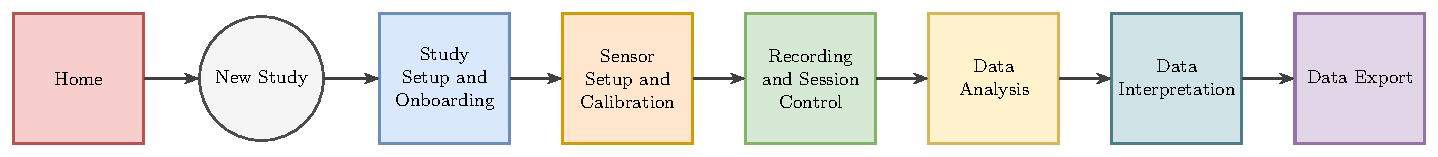
\includegraphics[max width=\linewidth,max totalheight=0.78\textheight]{diagrams/figure-3.1.pdf}\end{center}

\phantomsection\addcontentsline{lof}{figure}{\protect\numberline{3.1}The Sensa platform at a glance.}%
\textbf{Figure 3.1} The Sensa platform at a glance. Sensa is organized into six functional modules: study setup and onboarding, sensor calibration, session recording, data analysis, data interpretation, and data export
\end{figure}

The onboarding and calibration workflow was first designed as a high-fidelity prototype in Figma (Figma Inc., 2026), which allowed the information architecture, step sequencing, and interaction patterns to be defined and iterated before any code was written. It was then realized in the implemented platform, the working web frontend built by the development team, which follows that design. The prototype thus translates the fragmented multimodal study workflow into a structured, guided interface concept, defining how researchers move through setup, calibration, recording, analysis, and interpretation in a coherent sequence. The chapters that follow describe the design as realized, and the screenshots throughout are taken from the implemented platform rather than the prototype.

\hypertarget{authors-contribution}{%
\subsection{\texorpdfstring{3.3 Author's Contribution }{3.3 Author's Contribution }}\label{authors-contribution}}

The overall system logic of \emph{Sensa} was defined collaboratively with the team. Within that system, the onboarding and calibration workflow is the author\textquotesingle s individual contribution: the author defined the entire workflow and produced all of its interface designs.

This workflow guides the researcher through five sequential steps: (1) defining the study and selecting sensors and metrics; (2) confirming environmental and participant readiness; (3) calibrating the eye tracker with on-screen positioning and validating eye-tracking quality with real-time metrics; (4) placing biosensors, verifying signal connection, and recording a 30-second EDA baseline; and (5) confirming overall calibration readiness before recording begins. The eye-tracking validation performed within step (3) is described separately in Chapter 3.3.4, as it constitutes a distinct methodological contribution beyond the interface design.

The author\textquotesingle s contribution spans both design and implementation, which are distinguished here for clarity. At the design level, the author defined the complete onboarding and calibration workflow, including its information architecture, its screen-by-screen interaction flow, and all of its interface designs. These designs were produced within Sensa\textquotesingle s shared design language and UX standards, which were agreed jointly with the other contributors; the workflow therefore follows the same component conventions and visual style as the rest of the platform, while the workflow structure and the interaction decisions specific to it are the author\textquotesingle s own.

At the implementation level, the front-end and backend development of Sensa as a whole were led by other developers, but the author implemented several components of the workflow directly. These are: the real-time eye-tracking metrics (live-track box) shown during calibration positioning; the eye-tracking validation step (Chapter 3.3.4); the derived signal-quality indicators shown during EDA signal check and baseline recording, together with the live hub status indicator (Chapter 3.3.5). This implementation work was carried out with the assistance of an AI-based coding tool, Claude Code (Anthropic).

The prototype also integrates separately developed Sensa components that are not part of the author\textquotesingle s contribution, including the general recording modules, sensor output visualization, data cleaning, the EDA conversion and HDF5 storage pipeline, and the broader front-end and backend infrastructure developed by other contributors. The empirical evaluation in this thesis focuses specifically on the onboarding and calibration workflow designed and, in the components noted above, implemented by the author.

\hypertarget{study-setup-and-onboarding}{%
\subsubsection{3.3.1 Study Setup and Onboarding}\label{study-setup-and-onboarding}}

As seen in Figure 3.2, the user is initially prompted to define the study goal, the interface type (web or mobile application), the test environment (laboratory or remote setup), and the available hardware. The selectable study goals are: user effort and workload, emotional engagement/arousal, decision-making behaviour, and usability friction/interaction difficulty. These four goals were selected because they represent typical constructs in usability and user experience research that can be investigated through combinations of eye-tracking and physiological sensors (Aloi et al., 2024; Zhu \& Lv, 2023). They are the complete set of study goals supported by the current prototype; additional goals such as trust, learnability, aesthetic preference may be added in future development. These inputs collectively inform the sensor and metric recommendation that follows, as seen in Figure 3.3. For the purposes of this thesis, the focus is on the User Effort and Workload study goal and the user flow that stems from it. This goal was chosen to demonstrate the workflow because it is a common target in usability and HCI research and because it draws on multiple sensor types and on both behavioural and physiological indicators (for example fixation behaviour together with electrodermal arousal), which exercises the platform\textquotesingle s multimodal recommendation and calibration path more fully than a single-signal goal would.


\includegraphics[max width=\linewidth,max totalheight=0.78\textheight]{media/media/image12.png}\\
\phantomsection\addcontentsline{lof}{figure}{\protect\numberline{3.2}Study Setup screen.}%
\textbf{Figure 3.2} Study Setup screen. The user enters study details for documentation, which the system then uses to recommend appropriate sensors.

As seen in Figure 3.3, the user is presented with a list of recommended sensors and the specific metrics to track per sensor. The supported sensors are: eye tracking with the Tobii Eye Tracker 4C, plus EEG, EDA, and ECG via the Biosignalsplux sensor suite available at the HSRW Usability Lab. The user is also presented with a reason for why each sensor was recommended, along with contextual hints that guide researchers in interpreting their measurements.

These four modalities cover the principal constructs targeted by the supported study goals: fixation behaviour (eye tracking), cognitive load and attention (EEG), autonomic arousal and stress (EDA), and cardiovascular response to cognitive effort (ECG, via heart rate and heart rate variability). For each modality, the system surfaces the metric most commonly used to operationalise that construct in multi-sensor usability research (Aloi et al., 2024; Zhu \& Lv, 2023), which is what the recommendation is: a translation of a study goal into modality-appropriate measures, rather than a list of everything a sensor can produce. Fixation duration and gaze paths index where visual attention is allocated and how much search effort a task demands; an EEG-derived attention index serves as a proxy for cognitive engagement; heart rate variability is an established autonomic correlate of cognitive effort; and the mean EDA value is a standard index of sympathetic arousal.

For the User Effort and Workload goal used in this evaluation, workload is not observable in any single signal, so these four metrics are recommended together, each covering one facet of it: attentional cost in gaze, cognitive engagement in EEG, autonomic effort in HRV, and arousal in EDA. These are the same indicators shown to the researcher at goal selection (Figure 3.2), so the metric set the system recommends is visibly the set the chosen goal implies. This is the recommendation logic the platform is intended to demonstrate: the user states a goal, and the system, rather than the user, performs the mapping from that goal to the sensors and metrics that operationalise it.

The empirical evaluation in this thesis was limited to eye tracking and EDA, in order to keep the within-subjects sessions manageable and to test two distinct calibration procedures: spatial calibration for eye tracking and resting-baseline recording for EDA. EEG and ECG remain selectable interface options, reflecting the platform\textquotesingle s intended multimodal scope and demonstrating how the same goal-to-metric mapping extends across it, but they were not connected or measured during the evaluation (see Chapter 4.3). Sensor selection can also be performed manually if the researcher prefers to override the recommendation, as seen in Figure 3.4.

\begin{figure}[H]

\includegraphics[max width=\linewidth,max totalheight=0.78\textheight]{media/media/image5.png}

\phantomsection\addcontentsline{lof}{figure}{\protect\numberline{3.3}Recommended Sensors screen.}%
\textbf{Figure 3.3} Recommended Sensors screen. Based on the study goal selected during Study Setup, the system recommends a set of sensors and the metrics to track for each, together with a plain-language message explaining why those sensors were recommended and what to watch for.
\end{figure}

A central design challenge in the study setup flow is that sensor and metric selection requires domain knowledge that target users such as novice researchers or small teams may not possess. Selecting appropriate sensors for a given study goal, and choosing which metrics to track per sensor, presupposes familiarity with physiological measurement principles that cannot be assumed.

The Sensa design responds to this challenge in three complementary ways. First, at the study-goal selection step (Figure 3.2), each goal is shown alongside the physiological signal indicators most relevant to it (e.g., for User Effort and Workload: "alpha power down, fixations up, EDA up, HR up / RMSSD down"), enabling researchers to see at the goal-selection moment which signals each goal involves. Second, the system presents a recommended sensor set (Figure 3.3), accompanied by a goal-aware explanation under "Why these recommendations? that ties each recommended sensor to specific signals to watch for during the task. Third, a parallel manual sensor selection path (Figure 3.4) allows researchers who already know what they want to override the recommendation.

The recommendation logic is a predefined rule-based mapping between study goals, sensor modalities, and metrics, rather than a validated recommendation model. The mappings combine the literature-based indicators described above with the author\textquotesingle s own domain reasoning, and were not empirically validated against expert judgement or user outcomes.

In the current prototype the recommendation screen is implemented as a static demonstration: it is pinned to the User Effort and Workload goal used throughout the evaluation, and the same recommendation is shown irrespective of which goal is selected. Making the recommendation conditional on the selected study goal and the available hardware is the intended behaviour and remains to be implemented.

\begin{figure}[H]
\begin{center}
\includegraphics[width=0.775\linewidth]{media/media/image25.png}\end{center}

\phantomsection\addcontentsline{lof}{figure}{\protect\numberline{3.4}Manual Sensor Selection screen.}%
\textbf{Figure 3.4} Manual Sensor Selection screen. The user can customise which sensors to use and which metrics to track in their study.
\end{figure}

Together, these features support sensor selection decisions rather than only informing users about available sensors. The current build does not, however, include a validation mechanism that checks whether the user\textquotesingle s final selections are appropriate for the stated study goal; adding such a validation layer is identified as a direction for future development and noted as a limitation of the current prototype.

Figure 3.5 showcases the user's journey from the study setup to the readiness check phase.

\begin{figure}[H]
\begin{center}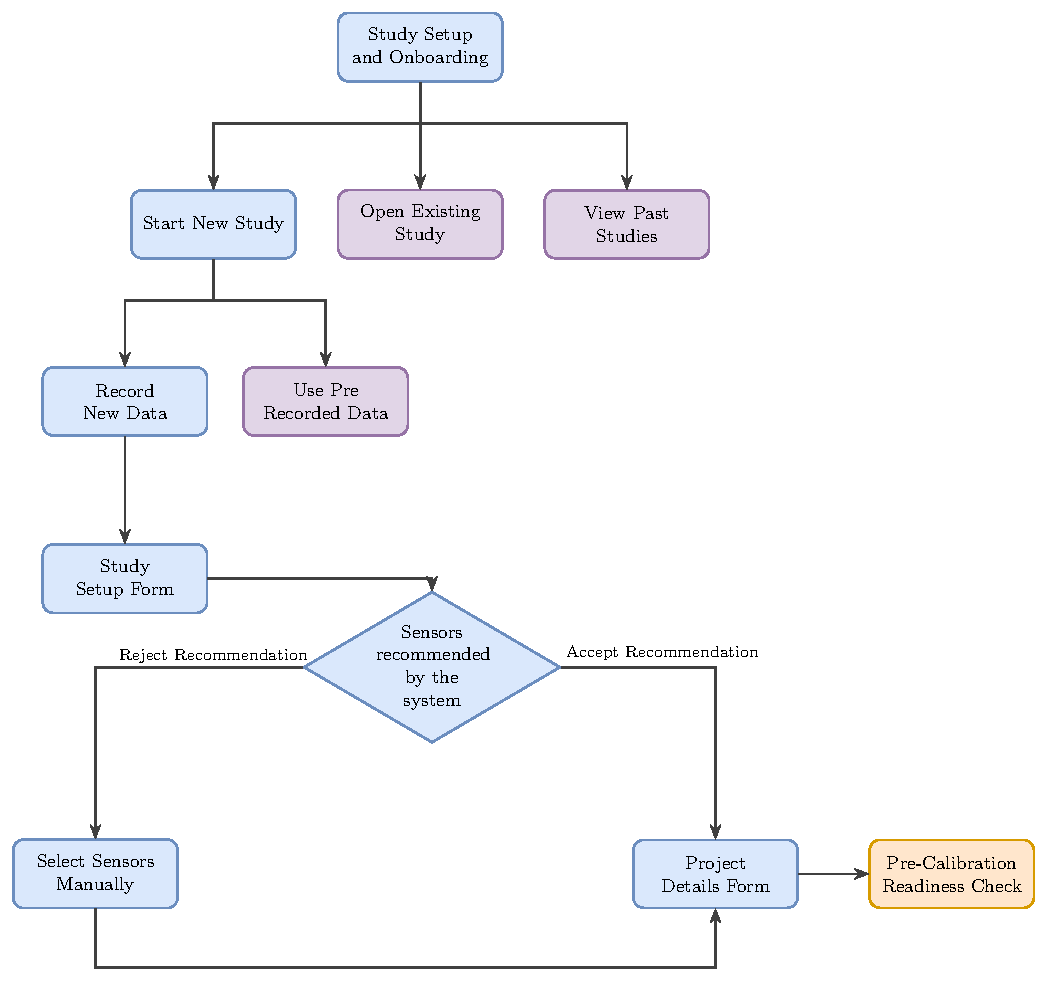
\includegraphics[max width=\linewidth,max totalheight=0.78\textheight]{diagrams/figure-3.5.pdf}\end{center}

\phantomsection\addcontentsline{lof}{figure}{\protect\numberline{3.5}Study setup and onboarding user flow.}%
\textbf{Figure 3.5} Study setup and onboarding user flow. The diagram traces the user\textquotesingle s journey from starting the study through to entering the readiness-check phase.
\end{figure}

\hypertarget{project-details-readiness-verification-and-calibration-overview}{%
\subsubsection{3.3.2 Project Details, Readiness Verification and Calibration Overview}\label{project-details-readiness-verification-and-calibration-overview}}

The session begins with a screen (Figure 3.6) displaying the study configuration and a prompt for the researcher to confirm the project name, participant count, and study objective (e.g: \emph{Identify usability issues in the checkout flow} or \emph{Measure participant cognitive and emotional responses during a task)} before proceeding to a readiness check.

\begin{figure}[H]

\includegraphics[max width=\linewidth,max totalheight=0.78\textheight]{media/media/image9.png}

\phantomsection\addcontentsline{lof}{figure}{\protect\numberline{3.6}Project Details screen.}%
\textbf{Figure 3.6} Project Details screen. The editable Study Configuration defined earlier sits at the top, followed by a form for documenting project-related details, with mandatory fields gated by inline error messages.
\end{figure}

A readiness checklist is presented, requiring the researcher to confirm the following pre-calibration conditions before sensor calibration begins (Figure 3.7):

\begin{itemize}
\item
  The participant is seated comfortably at the workstation with correct posture and at a distance of approximately 60 cm from the monitor. This distance represents the standard recommended operating range for the Tobii eye trackers, within which gaze detection accuracy and tracking stability are optimized (Dalrymple et al., 2018, p. 5). Deviations from this distance, whether the participant sits too close or too far from the screen, can reduce tracking quality and introduce systematic gaze error.
\item
  Room lighting and noise levels are consistent and adequate for biosensor and eye-tracking detection (Zhu \& Lv, 2023, p. 19).
\item
  All sensors are accessible and visible to the participant.
\item
  All biosensors have snap electrodes attached to them (single-use adhesive electrodes with a press-stud metal connector that clips onto the sensor cable).
\end{itemize}

\begin{figure}[H]
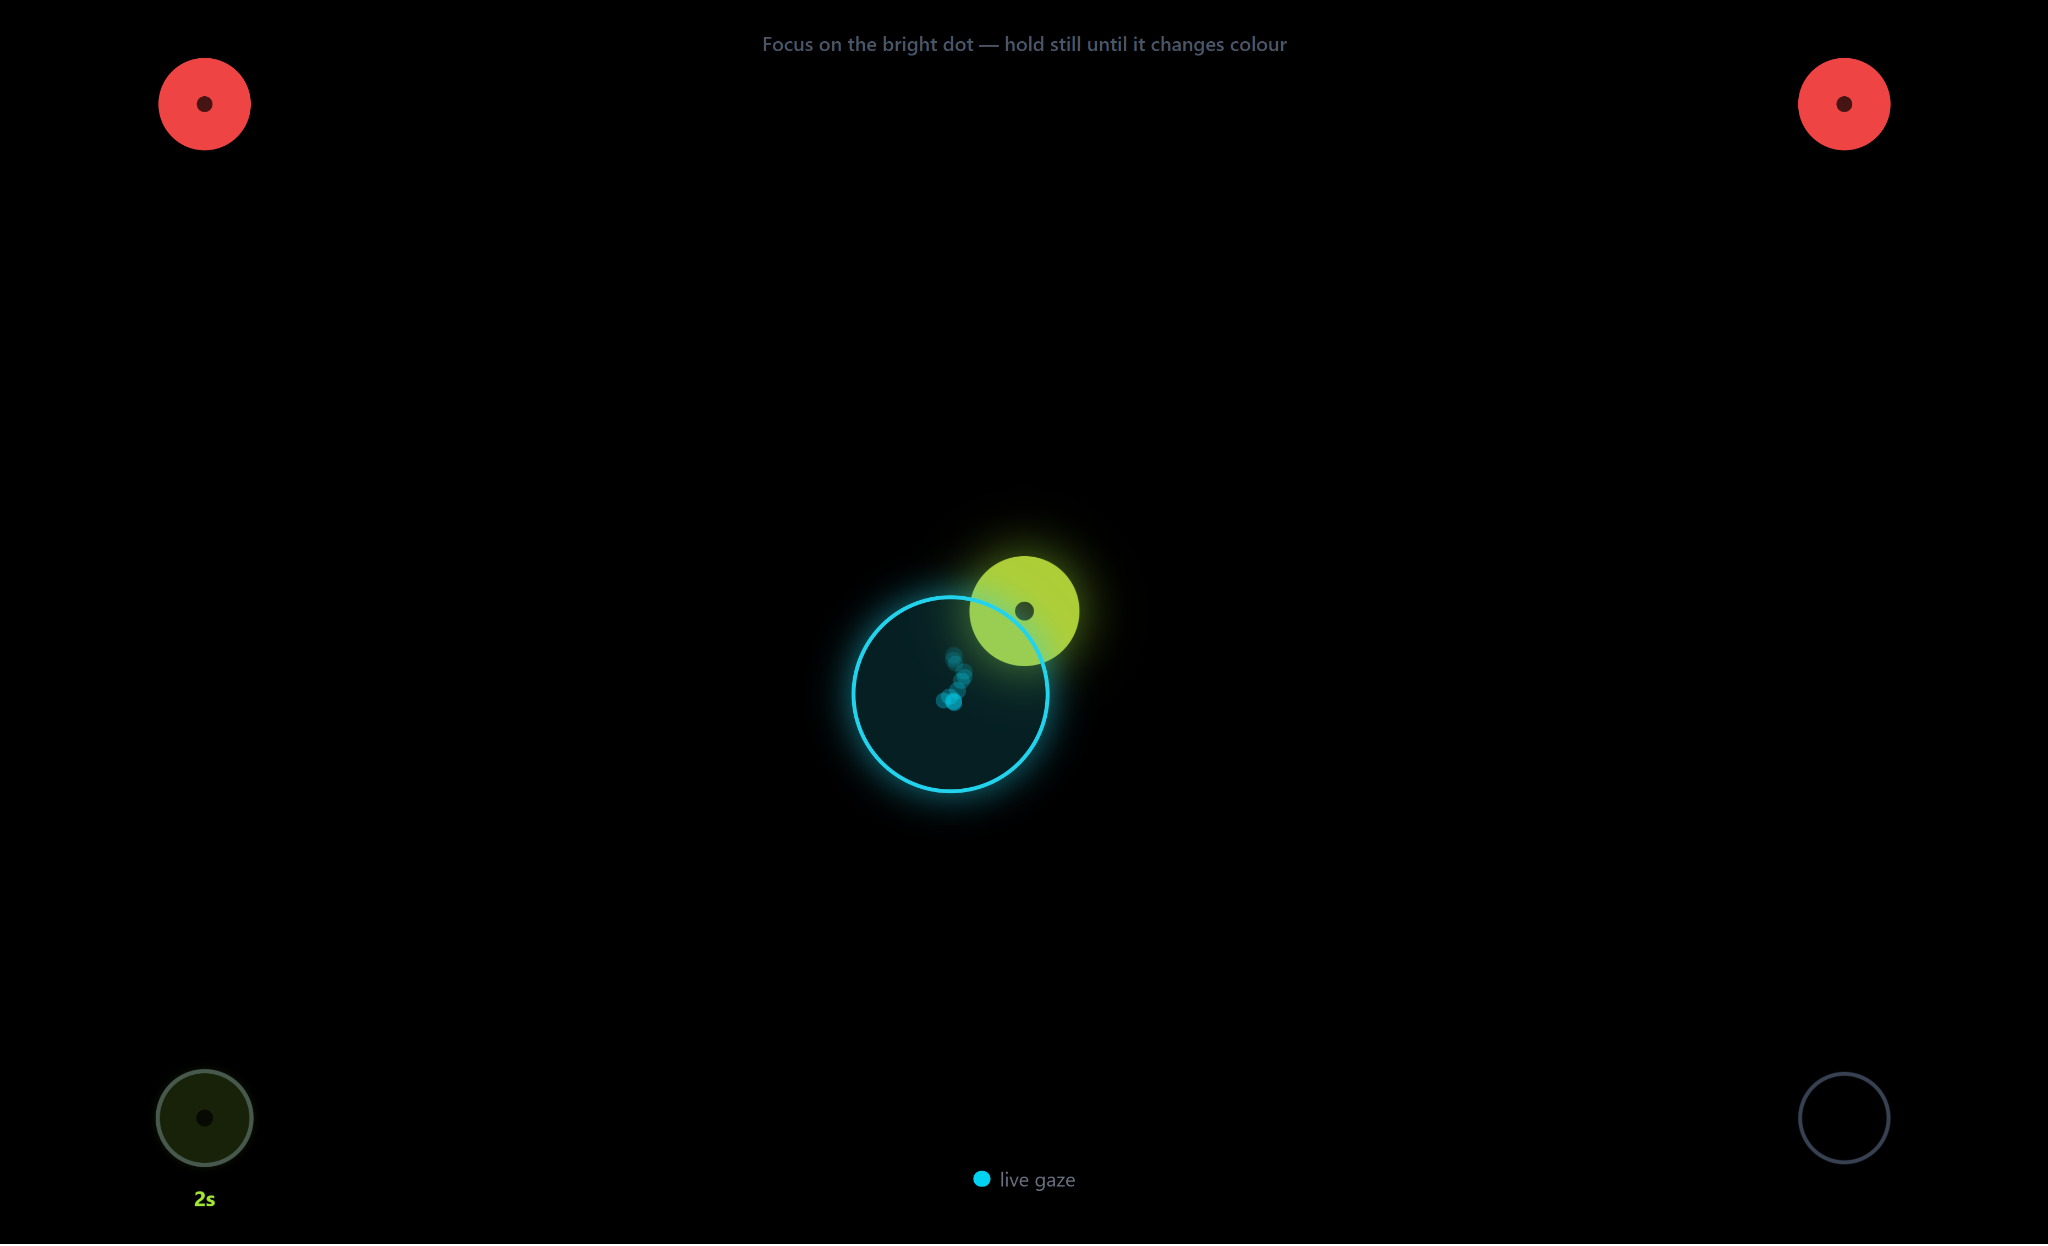
\includegraphics[max width=\linewidth,max totalheight=0.78\textheight]{media/media/image6.png}

\phantomsection\addcontentsline{lof}{figure}{\protect\numberline{3.7}Environment and Participant Readiness screen.}%
\textbf{Figure 3.7} Environment and Participant Readiness screen. The "Start Sensor Calibration" button is gated and remains disabled until every item in the checklist is checked off.
\end{figure}

The readiness checklist is the first of two preparatory phases; sensor-specific preparation, signal verification, and baseline recording are described in the per-sensor calibration flow that follows. The readiness checklist implements error prevention through prerequisite gating: the "Start Sensor Calibration" button remains disabled until all checklist items are confirmed, preventing users from entering calibration in an invalid state. As seen in Figure 3.8, a green success banner informs the user that the readiness check is complete once all items are marked in the checklist, and the primary button changes to an enabled state.

\begin{figure}[H]
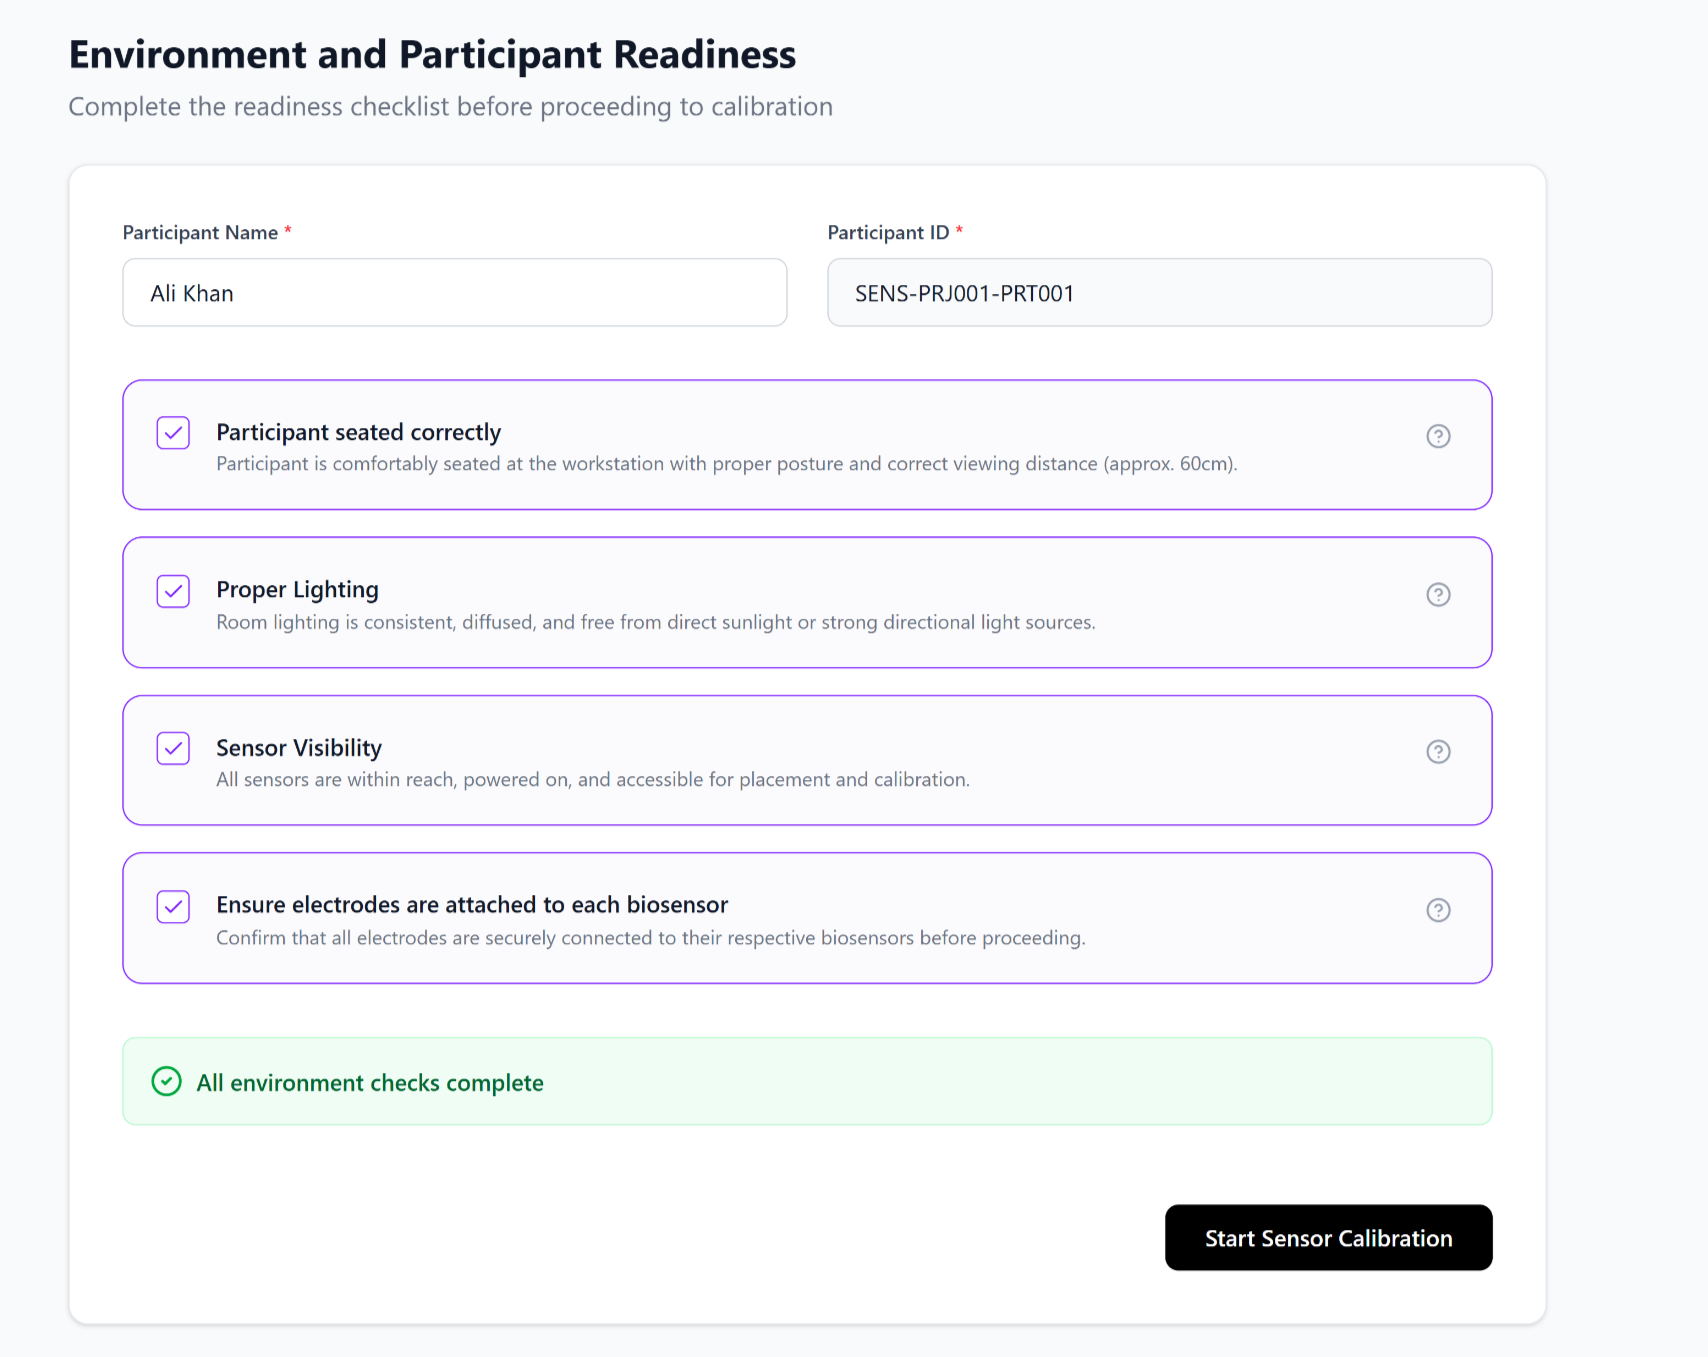
\includegraphics[max width=\linewidth,max totalheight=0.78\textheight]{media/media/image16.png}

\phantomsection\addcontentsline{lof}{figure}{\protect\numberline{3.8}Environment and Participant Readiness screen with all items checked.}%
\textbf{Figure 3.8} Environment and Participant Readiness screen with all items checked. A green success banner is shown and the "Start Sensor Calibration" button is now enabled.
\end{figure}

To support users without prior experience in verifying compliance with each condition, each checklist item includes an inline description and a clickable tooltip providing the relevant reference standard. For example, the seating item specifies the 60 cm viewing distance recommended for Tobii eye trackers, and the lighting item describes adequate ambient conditions for biosensor and eye-tracking detection. This approach embeds the domain knowledge required for self-assessment directly at the point of decision, reducing reliance on external manuals or prior training.

\begin{figure}[H]
\begin{center}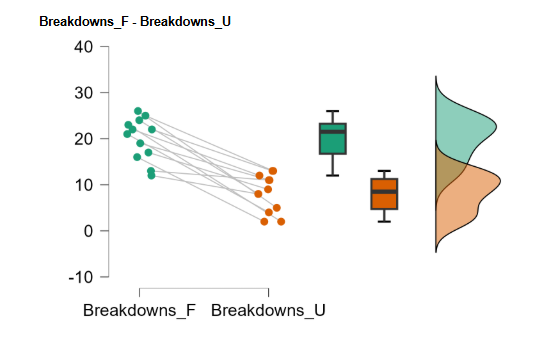
\includegraphics[width=0.775\linewidth]{media/media/image3.png}\end{center}

\phantomsection\addcontentsline{lof}{figure}{\protect\numberline{3.9}Calibration Overview screen.}%
\textbf{Figure 3.9} Calibration Overview screen. The "Proceed to Recording" button stays gated and disabled until all required sensors have been calibrated and set up.
\end{figure}

After the readiness check, the researcher is taken to the calibration page, where all connected sensors are listed as a checklist. The researcher calibrates each sensor individually by selecting it from the list (Figure 3.9). On-screen visual and written instructions guide calibration for each device.

\hypertarget{eye-tracker-calibration}{%
\subsubsection{3.3.3 Eye Tracker Calibration}\label{eye-tracker-calibration}}

As shown in Figure 3.10, eye-tracker calibration is presented as a guided four-step sequence: instructions, participant positioning, the calibration routine itself, and validation of the result. The first three steps are described here. The validation step, which constitutes a distinct methodological contribution rather than only an interface design, is described separately in Chapter 3.3.4.

\begin{figure}[H]
\begin{center}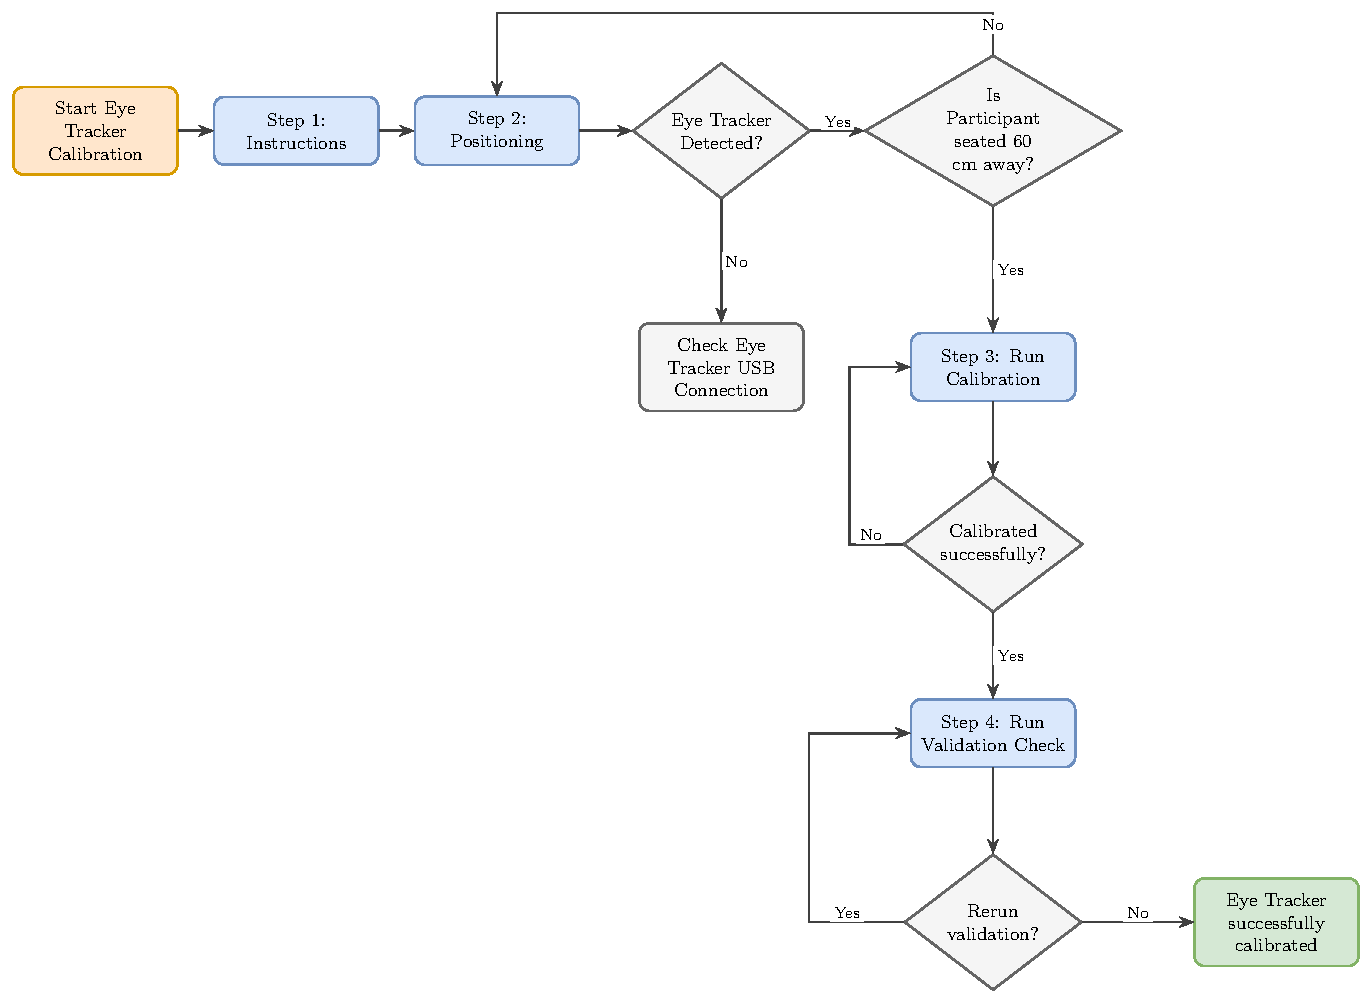
\includegraphics[max width=\linewidth,max totalheight=0.78\textheight]{diagrams/figure-3.10.pdf}\end{center}

\phantomsection\addcontentsline{lof}{figure}{\protect\numberline{3.10}Eye-tracker calibration subflow.}%
\textbf{Figure 3.10} Eye-tracker calibration subflow. The diagram traces the user\textquotesingle s journey from starting eye-tracker calibration through to a successful calibration.
\end{figure}

\textbf{Step 1: Instructions:} Calibration begins with a set of instructions accompanied by an illustration that informs the user to position themselves directly in front of the screen, at a distance of 60 cm while looking straight at the screen (Figure 3.11). This is used to prepare the user with guidance for the next step.

\begin{figure}[H]
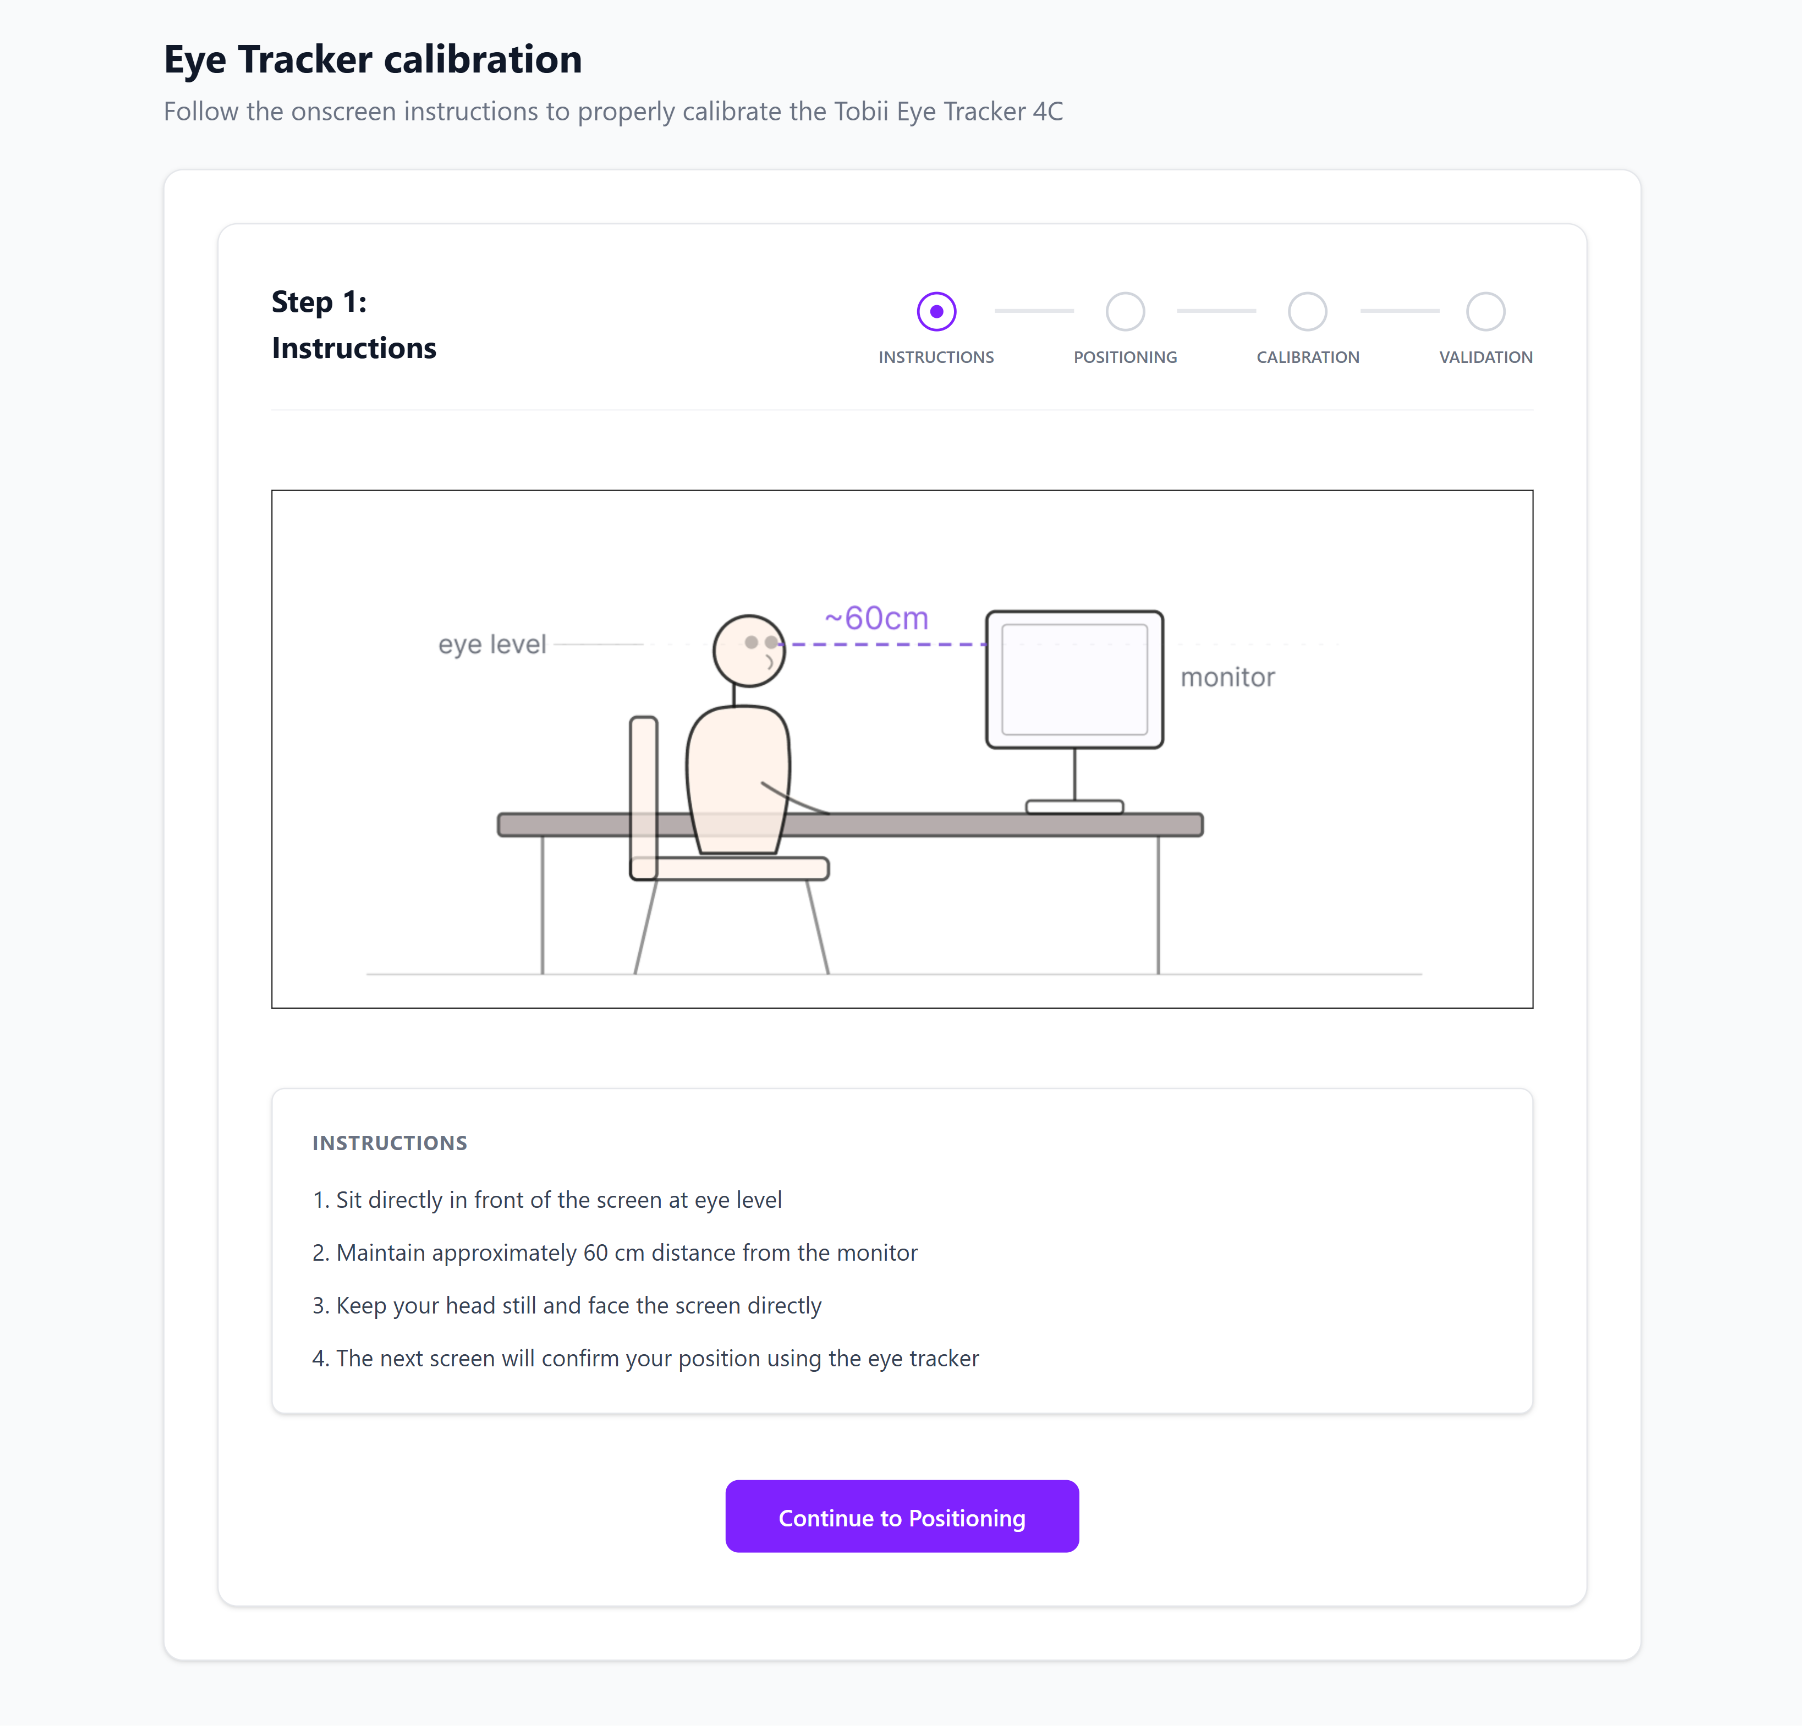
\includegraphics[max width=\linewidth,max totalheight=0.78\textheight]{media/media/image36.png}

\phantomsection\addcontentsline{lof}{figure}{\protect\numberline{3.11}Eye-tracking calibration, Step 1: Instructions.}%
\textbf{Figure 3.11} Eye-tracking calibration, Step 1: Instructions. An illustrated set of instructions directs the user to sit directly in front of the screen, at 60 cm, looking straight ahead, preparing them for the positioning step.
\end{figure}

\textbf{Step 2: Positioning:} Calibration begins with a positioning screen that provides live track-box feedback. The track box is the three-dimensional volume in front of the tracker within which the Tobii 4C can see both eyes; the screen shows the participant\textquotesingle s eyes as points inside this volume in real time (Figure 3.12 and Figure 3.13), confirming that the participant is seated within the optimal detection range before any calibration targets are displayed before moving on to the actual calibration. Correct head position is a precondition for a usable calibration, since a participant who sits too close, too far, or off-axis can produce degraded tracking regardless of how the calibration itself proceeds. The screen guides the participant through two states: an out-of-range state that prompts the participant to correct their position (Figure 3.13), and an in-range confirmation that enables progression to calibration (Figure 3.14). Gating progression on correct positioning is another instance of error prevention (see Chapter 3.6): the participant cannot begin calibration from an invalid starting position. Additionally, the live eye-tracker status card underneath the live-track box (see lower part of Figure 3.13) keeps the user informed about the connection status of the eye-tracker.

\begin{figure}[H]

\includegraphics[max width=\linewidth,max totalheight=0.78\textheight]{media/media/image18.png}

\phantomsection\addcontentsline{lof}{figure}{\protect\numberline{3.12}Eye-tracking calibration, Step 2: Positioning, with the user outside the optimal range.}%
\textbf{Figure 3.12} Eye-tracking calibration, Step 2: Positioning, with the user outside the optimal range. The live track box shows the user seated outside the recommended 60 cm range, so the "Go to Calibration" button is disabled and the current distance to the eye tracker is displayed in millimetres. The status card below reports the connection state (Device Connected or Not Connected), the eye-tracker model and serial number, and the live distance.
\end{figure}

\begin{figure}[H]

\includegraphics[max width=\linewidth,max totalheight=0.78\textheight]{media/media/image14.png}

\phantomsection\addcontentsline{lof}{figure}{\protect\numberline{3.13}Eye-tracking calibration, Step 2: Positioning, with the user within the optimal range.}%
\textbf{Figure 3.13} Eye-tracking calibration, Step 2: Positioning, with the user within the optimal range. The user is seated within the recommended 60 cm range, so the "Go to Calibration" button is enabled. The status card below reports the connection state (Device Connected or Not Connected), the eye-tracker model and serial number, and the live distance.
\end{figure}

\textbf{Step 3: Calibration routine:} Once positioning is confirmed, the participant is shown a pre-calibration screen that explains what is about to happen (Figure 3.14). Due to hardware availability limitations and being restricted to using a Tobii 4C Eye-tracker which is not compatible with the Tobii Pro SDK required to implement calibration directly within Sensa, the calibration layer could not run natively in Sensa, and hence the screen directs the user to Tobii's native calibration sequence. Sensa does not reimplement gaze estimation; the calibration routine is run through the Tobii, which builds and stores the gaze model. The rationale for this boundary, and what it means for how calibration quality is then measured, is set out in Chapter 3.3.4.

\begin{figure}[H]

\includegraphics[max width=\linewidth,max totalheight=0.78\textheight]{media/media/image30.png}

\phantomsection\addcontentsline{lof}{figure}{\protect\numberline{3.14}Eye-tracking calibration, Step 3: Calibration, pre-calibration screen.}%
\textbf{Figure 3.14} Eye-tracking calibration, Step 3: Calibration, pre-calibration screen. The screen directs the user to Tobii Core's native calibration routine, sets out instructions for the upcoming step, and lets the user set the pass threshold for the validation layer.
\end{figure}

After calibration, the system prompts the user to run a validation check and, if the resulting calibration quality is insufficient, prompts recalibration. Since this measurement is the methodological core of the author\textquotesingle s contribution, it is treated separately in the next chapter.

\hypertarget{the-eye-tracker-validation-layer}{%
\subsubsection{\texorpdfstring{3.3.4 The Eye-Tracker Validation Layer }{3.3.4 The Eye-Tracker Validation Layer }}\label{the-eye-tracker-validation-layer}}

\hypertarget{rationale}{%
\paragraph{3.3.4.1 Rationale}\label{rationale}}

A calibration routine maps (in this case, routed through Tobii's Core software) a participant\textquotesingle s eye images five points on the screen (centre, and on the four edges). This data is used to interpolate the gaze coordinates for the other points on screen. However, completing a calibration does not by itself guarantee that the resulting gaze estimates are accurate. Calibration quality varies with eye physiology, ambient lighting, head position, and the calibration procedure itself, and must therefore be measured, through an explicit validation step carried out before any data collection begins (Nyström et al., 2013, p. 286). A separate validation step, in which targets are presented at known locations and the recorded gaze is compared against them, is the standard method for obtaining an objective, reportable measure of data quality. In practice, empirically measured accuracy often differs from manufacturer-reported specifications (Dalrymple et al., 2018, p. 9).

The validation layer described here was designed to address this gap by providing a transparent, hardware-grounded assessment of the calibration produced by the Tobii runtime. The use of a consumer-grade eye tracker further reinforces the need for this validation step. It quantifies calibration quality and reports the results using the standard metrics and units employed in the eye-tracking literature.

The Tobii 4C builds and stores its gaze model through the manufacturer\textquotesingle s own runtime and reports no numeric accuracy or precision back to the operator (Dell Inc., 2016, p. 6). Meanwhile, its native validation is a qualitative gaze-trace visualization (Dell Inc., 2016, p. 9). An operator using the device alone therefore has no objective measure of how good a given calibration is. The validation layer described here was built to close that gap: a transparent, hardware-grounded measurement that quantifies the quality of whatever calibration the Tobii runtime has produced, and reports it in the units conventional to the field.

\hypertarget{measured-quantities}{%
\paragraph{3.3.4.2 Measured quantities}\label{measured-quantities}}

The layer reports the two quantities into which eye-tracking data quality is conventionally decomposed (Dalrymple et al., 2018, p. 9; Nyström et al., 2013, p. 281):

\begin{itemize}
\item
  \textbf{Accuracy}: the systematic offset between the target\textquotesingle s true location and the mean recorded gaze position, capturing bias.
\item
  \textbf{Precision}: the reliability, or variation, of repeated gaze samples about their own mean, capturing noise independently of whether the mean is correctly located.
\end{itemize}

Both are reported in degrees of visual angle, which normalizes the measurement for display size and viewing distance so that a quality figure is comparable across setups. The validation layer additionally reports valid data yield (the proportion of collected samples containing a valid binocular estimate), per-target accuracy, first-pass calibration success, and recalibration count. These results are presented to the user on the validation results screen (Chapter 3.3.4.5).

\hypertarget{the-five-point-validation-grid-and-gaze-trace}{%
\paragraph{3.3.4.3 The five-point validation grid and gaze trace}\label{the-five-point-validation-grid-and-gaze-trace}}

During validation the five targets are presented one at a time as an overlay on the display, following the introductory prompt shown in Figure 3.15. Each target appears as a highlighted point that the participant is asked to look at, and a live gaze trace follows the participant\textquotesingle s eyes across the screen throughout, providing continuous feedback that the eyes are being tracked (Figure 3.16). Each target is held for approximately two seconds, comprising a brief settling period that allows the eye to reach the new location followed by approximately 1.5 seconds during which the binocular gaze samples for that target are collected, with an on-screen countdown indicating the remaining dwell time.

\begin{figure}[H]
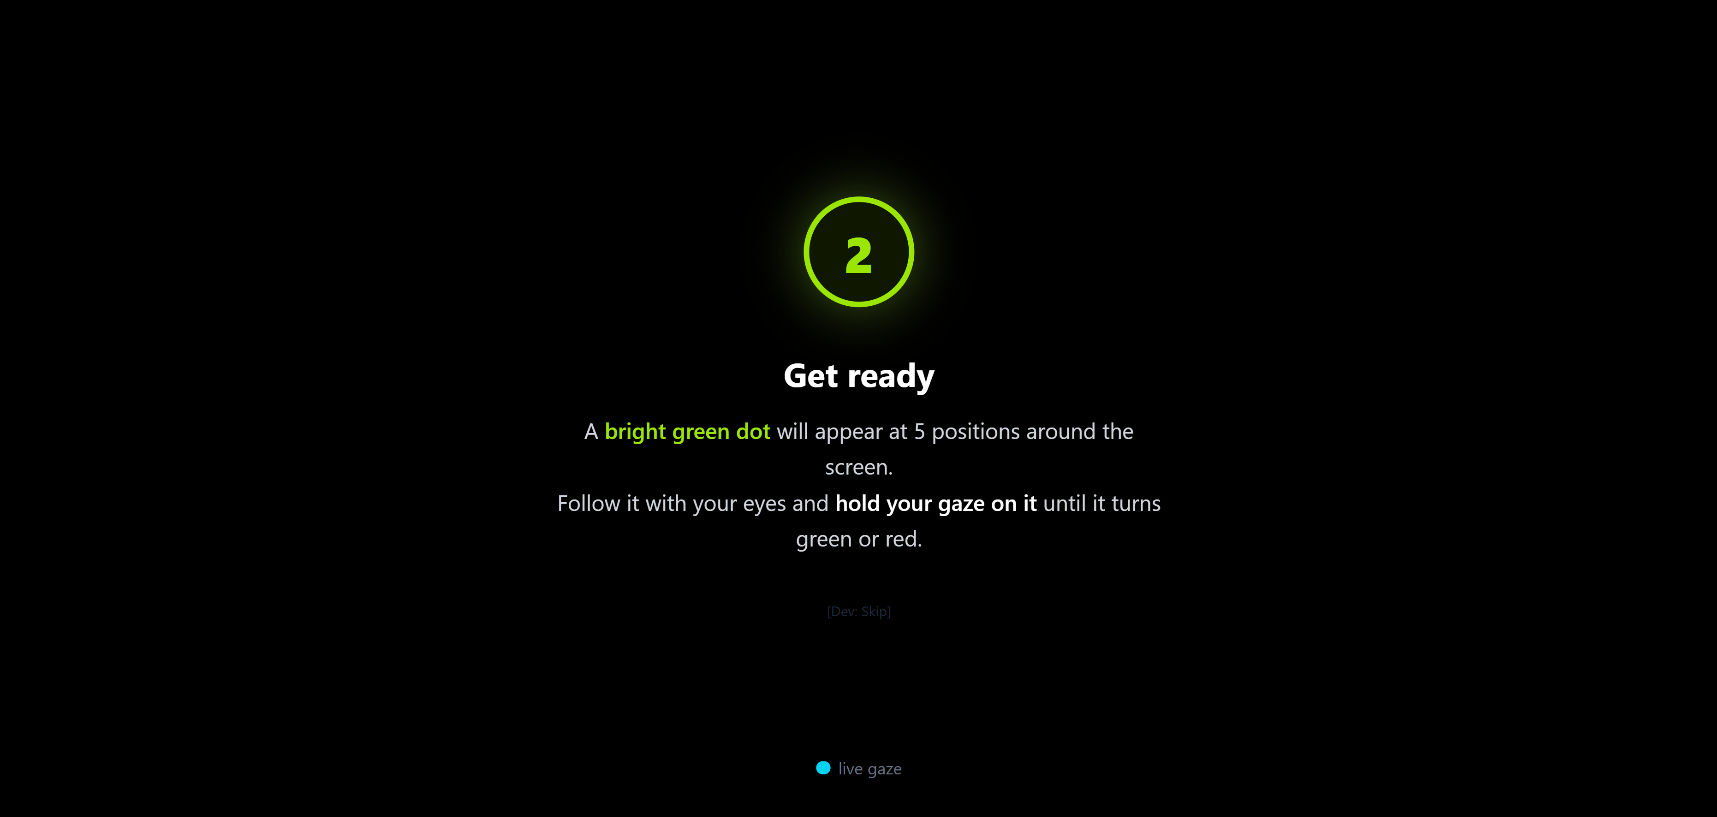
\includegraphics[max width=\linewidth,max totalheight=0.78\textheight]{media/media/image34.png}

\phantomsection\addcontentsline{lof}{figure}{\protect\numberline{3.15}Eye-tracking calibration, Step 4: Validation, instructions overlay.}%
\textbf{Figure 3.15} Eye-tracking calibration, Step 4: Validation, instructions overlay. The overlay tells the user what to expect (a bright dot appearing at five points around the screen) and what to do (follow the dot and hold their gaze on it until it turns red or green).
\end{figure}

The five targets are presented at fixed, normalized display coordinates: the four corners of the usable display area, inset slightly from the edges, and the centre. Only samples that contain a valid estimate from both eyes are used for the position estimate; samples in which neither eye returns a valid estimate are discarded and counted towards the valid-data yield rather than towards the position estimate.

\begin{figure}[H]

\includegraphics[max width=\linewidth,max totalheight=0.78\textheight]{media/media/image22.png}

\phantomsection\addcontentsline{lof}{figure}{\protect\numberline{3.16}Eye-tracking calibration, Step 4: Validation, five-point grid.}%
\textbf{Figure 3.16} Eye-tracking calibration, Step 4: Validation, five-point grid. The five targets are presented one at a time while a live gaze trace follows the user\textquotesingle s eyes across the screen. Holding gaze on a target for two seconds turns it green for success; red indicates failure.
\end{figure}

As soon as a target\textquotesingle s collection window closes, the point changes colour to communicate its outcome: it turns green when the mean recorded gaze for that target falls within the pass threshold (explored further in Chapter 3.3.4.4), and red when the gaze falls outside the threshold or too few valid samples were captured. By the end of the procedure, the complete set of colour-coded results provides an immediate visual summary of calibration quality. This immediate, visible feedback is a further application of the visibility-of-system-status principle (Nielsen, 1994) and supports the decision of whether recalibration is necessary, as the presence of one or more red targets indicates that the calibration should be repeated before proceeding.

\hypertarget{measuring-accuracy-and-prescions}{%
\paragraph{\texorpdfstring{3.3.4.4 Measuring accuracy and prescions }{3.3.4.4 Measuring accuracy and prescions }}\label{measuring-accuracy-and-prescions}}

The main methodological improvement in this layer is the calculation of gaze accuracy and precision during validation: on-screen error is converted into visual angle at the eye rather than reported as raw screen distance.

As shown in Figure 3.17, the gaze samples collected for each target are first averaged to obtain a single recorded gaze position. Each raw sample that contains a valid estimate from both eyes is reduced to a single binocular gaze point by averaging the left and right on-screen coordinates. These points are then averaged over the collection window to obtain the mean recorded gaze position for the target. During validation the system then compares this mean recorded gaze position with the known position of the target, producing an on-screen error (for example in pixels or millimetres).

\begin{figure}[H]
\begin{center}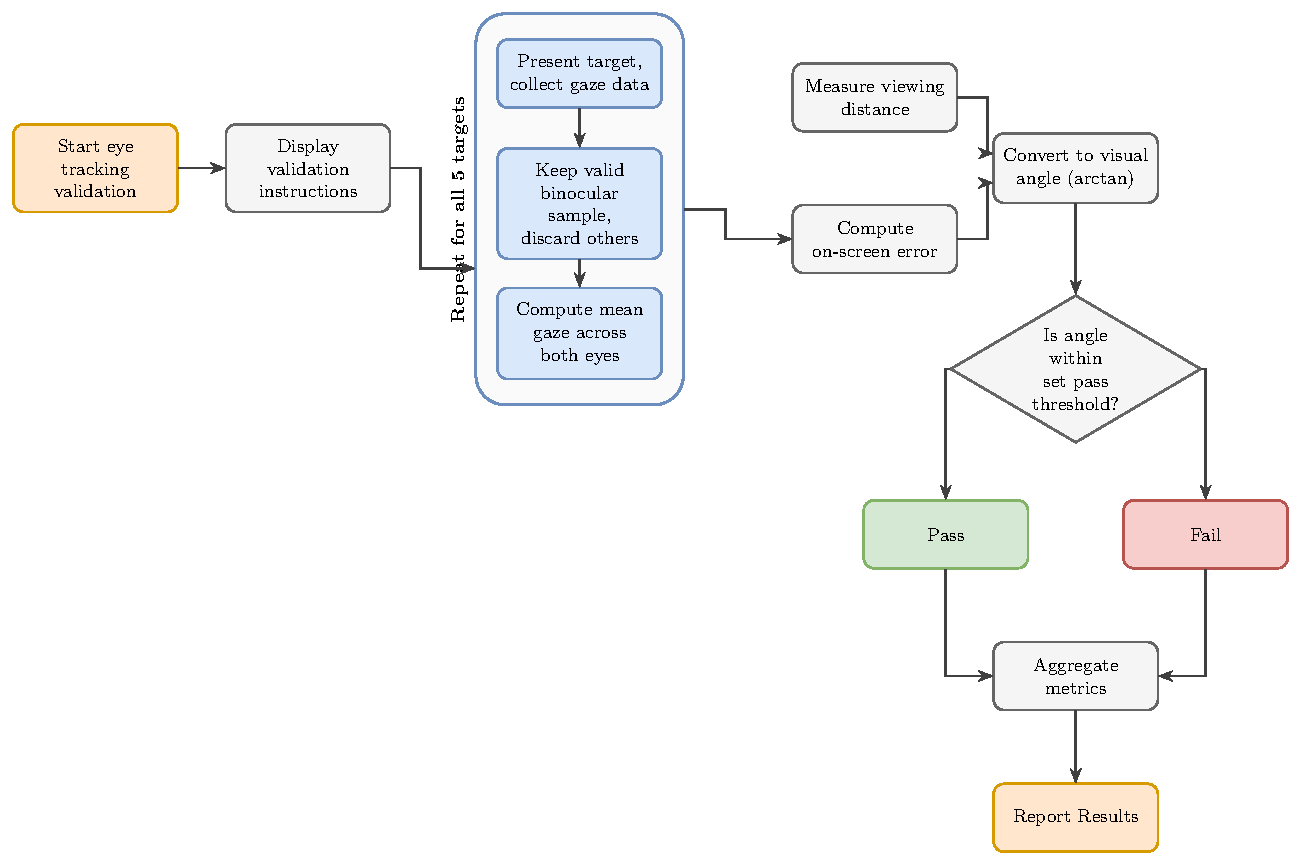
\includegraphics[max width=\linewidth,max totalheight=0.78\textheight]{diagrams/figure-3.17.pdf}\end{center}

\phantomsection\addcontentsline{lof}{figure}{\protect\numberline{3.17}Eye-tracking measurement pipeline.}%
\textbf{Figure 3.17} Eye-tracking measurement pipeline. The system measures the user\textquotesingle s viewing distance live from the eye-position stream, presents the five targets and collects binocular gaze at each, and computes the per-target on-screen error. It converts this error to degrees of visual angle as the inverse tangent of the error over the measured distance, then reports accuracy, precision, and valid data yield and scores each target as pass or fail against the pass threshold (maximum permissible mean accuracy).
\end{figure}

On-screen error alone is not enough, because the same distance on screen corresponds to a larger visual angle when the participant sits closer to the monitor and a smaller one when they sit further away. To account for this, the system does not assume a fixed viewing distance. It reads the participant\textquotesingle s eye position live from the tracker, uses this to estimate their actual distance from the screen, and converts the on-screen error into degrees of visual angle as the inverse tangent of the error over that distance.

\textbf{Accuracy} is computed per target as the angular offset between the mean recorded gaze and the known target position. The normalized error is scaled to a physical on-screen distance using the known display width and then converted to a visual angle by taking the inverse tangent of that distance over the measured viewing distance:

\[ \text{error} = \sqrt{(\text{meanGazeX} - \text{targetX})^{2} + (\text{meanGazeY} - \text{targetY})^{2}} \]

\[ \text{accuracy}\,(^{\circ}) = \arctan\!\left(\frac{\text{error} \times W}{d}\right) \]

where W is the physical display width in millimetres and d is the participant\textquotesingle s viewing distance in millimetres, measured live as described above. The overall accuracy for a session is the mean of the per-target values across the valid targets. Defining accuracy as the offset of the recorded gaze location from the target, averaged over the targets, follows Nyström et al. (2013, p. 280). Its decomposition from precision and its expression in degrees of visual angle follows the standard treatment in the eye-tracking methodology literature (Holmqvist et al., 2012, p. 48).

\textbf{Precision} describes how closely the individual gaze samples cluster around their mean, independently of how far that mean lies from the target. For each target, precision is calculated as the root-mean-square distance of the (N) valid binocular gaze samples from their mean position:

\[ \text{spread} = \sqrt{\frac{1}{N} \sum \left((\text{sampleX} - \text{meanGazeX})^{2} + (\text{sampleY} - \text{meanGazeY})^{2}\right)} \]

The resulting spread is then converted into degrees of visual angle using the same relationship as for accuracy:

\[ \text{precision}\,(^{\circ}) = \arctan\!\left(\frac{\text{spread} \times W}{d}\right) \]

Here, (W) is the physical display width, (d) is the measured viewing distance, and the summation includes all valid binocular samples collected for the target. The summation Σ runs over the N valid binocular samples collected for the target. This standard-deviation form is one of the two dispersion estimators recommended for spatial precision; the alternative expresses precision as the root-mean-square of the distances between temporally successive samples as used by Nyström et al. (2013, p. 280) and described by Holmqvist et al. (2012, p. 48). This measure is used because it captures the overall spatial stability of the fixation rather than the variation between consecutive gaze samples.

Reporting accuracy, precision, and valid-data yield together follows the standardized data-quality report proposed by the latter authors (Holmqvist et al., 2012, p. 49). Valid data yield is the proportion of collection samples containing a valid binocular estimate, N\_valid/N\_all (Nyström et al., 2013, p. 280).

\textbf{The pass threshold} is a maximum permissible mean accuracy, expressed in degrees of visual angle and set to 3 degrees by default. This threshold is configurable by the user (Figure 3.14) during Step 3 of eye-tracker calibration and reported together with the result in Step 4. The 3 degrees is pragmatic default rather than a fixed standard. Acceptance criteria in eye tracking are study- and hardware-dependent: research-grade systems are typically validated to below one degree, whereas consumer trackers such as the Tobii 4C realistically achieve coarser accuracy under non-laboratory seating and lighting. Mikalef et al. (2023, p .4) set a validation-accuracy threshold of 2.5 degrees for a consumer eye tracker, describing it as an acceptable error margin corresponding to fewer than ten pixels at a viewing distance of 50 to 70 cm. The 3-degree default adopted here sits slightly above that value, providing a usable readiness gate for a consumer device operated by a non-expert rather than a research-grade acceptance criterion. Since the threshold is user-configurable and reported alongside every result, the pass criterion is explicit and can be tightened for stricter applications.

The pass/fail decision is based on angular accuracy alone. A target passes if it returns valid gaze data and its accuracy is within the defined threshold, and the session passes if all five targets return valid data and the mean accuracy across them is within the threshold. Precision and valid-data yield are reported to help interpret the result but do not contribute to the pass/fail outcome.

Two simplifications of this real-time implementation should be stated.

First, the metrics are computed over all valid samples in each collection window rather than over an algorithmically detected fixation. This avoids dependence on a fixation-detection algorithm, whose choice can materially change the resulting values (Holmqvist et al., 2012, p. 50), but it may include saccadic samples where present. It distinguishes the present procedure from Nyström et al. (2013, p. 280), who apply fixation detection and additional sample-selection criteria before computing the same quantities.

Second, the tracker reports gaze in normalized display coordinates, with the horizontal component normalized by display width and the vertical by display height. The implementation forms a single normalized Euclidean error from the two components and scales it by the display width alone, rather than converting each component to millimetres separately. On a 16:9 display this overestimates any error carrying a vertical component, by a factor of up to 1.78 for a purely vertical error, while leaving purely horizontal errors unaffected. Reported accuracy and precision values are therefore inflated by a systematic, direction-dependent factor. Because the same instrument and conversion are applied in both conditions, this inflation is expected to be similar across conditions and to substantially offset in the within-participant paired comparison on which H5 is evaluated. It would cancel exactly only if the distribution of error directions were identical across conditions, which cannot be assumed; the offset is therefore approximate rather than exact. This limitation reinforces that the reported values are instrument-relative rather than absolute ground truth (Chapters 3.3.4.6, 4.4.3, and 4.7.4).

The author defined the methodological decisions behind this process (live distance measurement, binocular data reduction, angular error conversion, and the validation threshold) and verified the outputs against the hardware and the eye-tracking literature.

\hypertarget{result-visualisation-and-pass-criteria}{%
\paragraph{3.3.4.5 Result visualization and pass criteria}\label{result-visualisation-and-pass-criteria}}

The validation results are shown in a two-dimensional scatter plot in normalized display coordinates (Figures 3.18 and 3.19). The plot shows the five target positions and their corresponding mean gaze positions, with dashed lines indicating the offset between each target and the recorded gaze. The length of each offset line is the visual representation of the accuracy error. Elements are colour-coded against the pass threshold, shown in green when within the predefined acceptance limit and in red when exceeding it. This lets the operator see at a glance both the magnitude and the spatial pattern of any systematic offset, for example a consistent downward displacement indicating a vertical bias. A target passes if its accuracy is within the pass threshold (3 degrees of visual angle by default, as defined in Section 3.3.4.4). The session passes if a sufficient number of targets are valid and the mean accuracy across valid targets is within the threshold.Presenting the measurement outcome visibly and immediately follows established usability guidance on visibility of system status (Nielsen, 1994).

\begin{figure}[H]
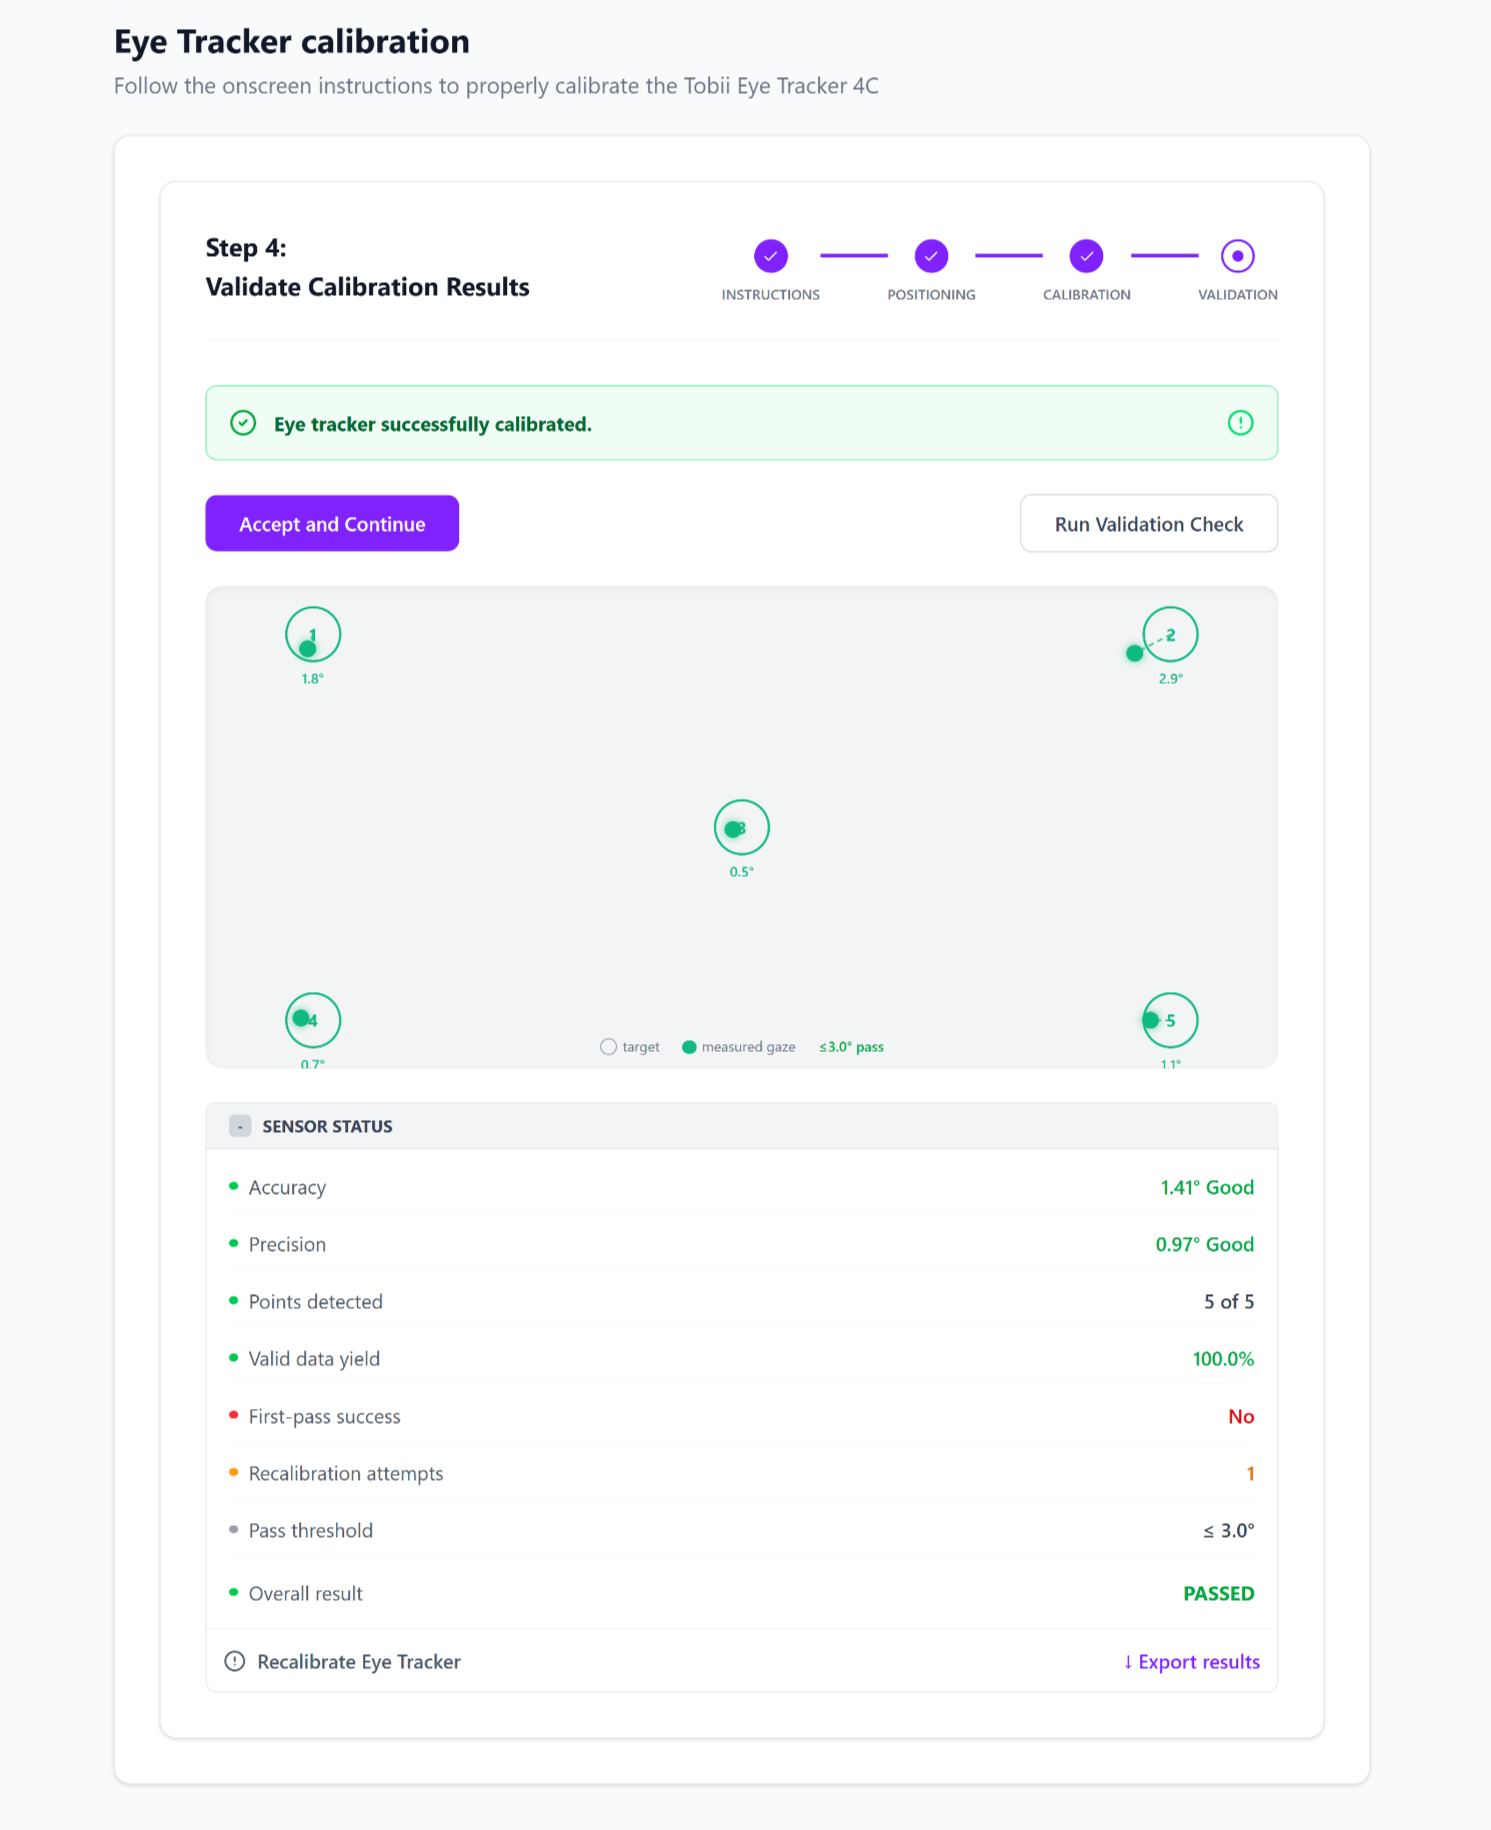
\includegraphics[max width=\linewidth,max totalheight=0.78\textheight]{assets/figure-3.18.png}

\phantomsection\addcontentsline{lof}{figure}{\protect\numberline{3.18}Eye-tracking calibration, Step 4: Validation, showing a successful calibration.}%
\textbf{Figure 3.18} Eye-tracking calibration, Step 4: Validation, showing a successful calibration. A green success banner sits above a scatter plot of the five-point grid, showing the intended gaze target against the computed gaze position for each point. A collapsible table below reports the colour-coded metrics: gaze accuracy, gaze precision, valid data yield, points detected, recalibration attempts, the pass threshold, and the overall result.
\end{figure}

This is why, post validation, the user is presented with a colour coded banner message at the top indicating whether the calibration quality was good (green) or prompts the user to perform calibration again (red) above the scatter plot.

Underneath the scatter plot, the user is also presented with numerical outputs for each calibration-quality metric, namely: gaze accuracy and gaze precision in degrees, valid data yield as a percentage, the number of points detected, whether the calibration succeeded on the first attempt, the number of recalibration attempts, the pass threshold, and the overall calibration status (pass or fail), as seen Figure 3.18 and Figure 3.19, along with a colour coded banner message at the top indicating success or failure of the validation.

\begin{figure}[H]

\includegraphics[max width=\linewidth,max totalheight=0.78\textheight]{media/media/image31.png}

\phantomsection\addcontentsline{lof}{figure}{\protect\numberline{3.19}Eye-tracking calibration, Step 4: Validation, showing a failed calibration.}%
\textbf{Figure 3.19} Eye-tracking calibration, Step 4: Validation, showing a failed calibration. As in Figure 3.18, but a red error banner reports the failure and prompts recalibration, above the same five-point scatter plot and the same collapsible table of colour-coded metrics.
\end{figure}

\hypertarget{system-boundary}{%
\paragraph{3.3.4.6 System boundary}\label{system-boundary}}

In both the unified and fragmented conditions, gaze estimation is performed by the Tobii eye tracker and the Tobii Stream Engine, while Sensa\textquotesingle s validation layer only evaluates the resulting gaze data by comparing recorded gaze positions with known validation targets. This separation is intentional: it allows the validation process to function as an independent assessment step rather than as part of the calibration method being compared.

It must be noted that Sensa\textquotesingle s validation procedure is custom-built and has not been validated against a reference-grade eye tracker, thus the reported accuracy values should not be interpreted as absolute ground-truth measurements. Instead, they should be understood as values relative to this specific validation setup. This limitation is addressed in the results discussion and revisited in the Limitations chapter.

\hypertarget{biometric-sensor-calibration}{%
\subsubsection{\texorpdfstring{3.3.5 Biometric Sensor Calibration }{3.3.5 Biometric Sensor Calibration }}\label{biometric-sensor-calibration}}

To ensure consistency in design, as shown in Figure 3.20, the biometric sensor calibration also follows a consistent four-step pattern, visible a stepper across the top of every screen (Placement, Connect, Signal Check, Baseline), always keeping the researcher informed of which step is active and what remains. The flow is described here for the electrodermal activity (EDA, or GSR) sensor, the biosignal modality scored in this study; the same four-stage structure is applied to the other supported biosensors. As with the readiness checklist and eye-tracker positioning, each step gates progression: the researcher cannot advance until the current stage\textquotesingle s requirements are confirmed, which prevents baseline recording from an improperly prepared or disconnected state (error prevention; see Chapter 3.6).

\begin{figure}[H]
\begin{center}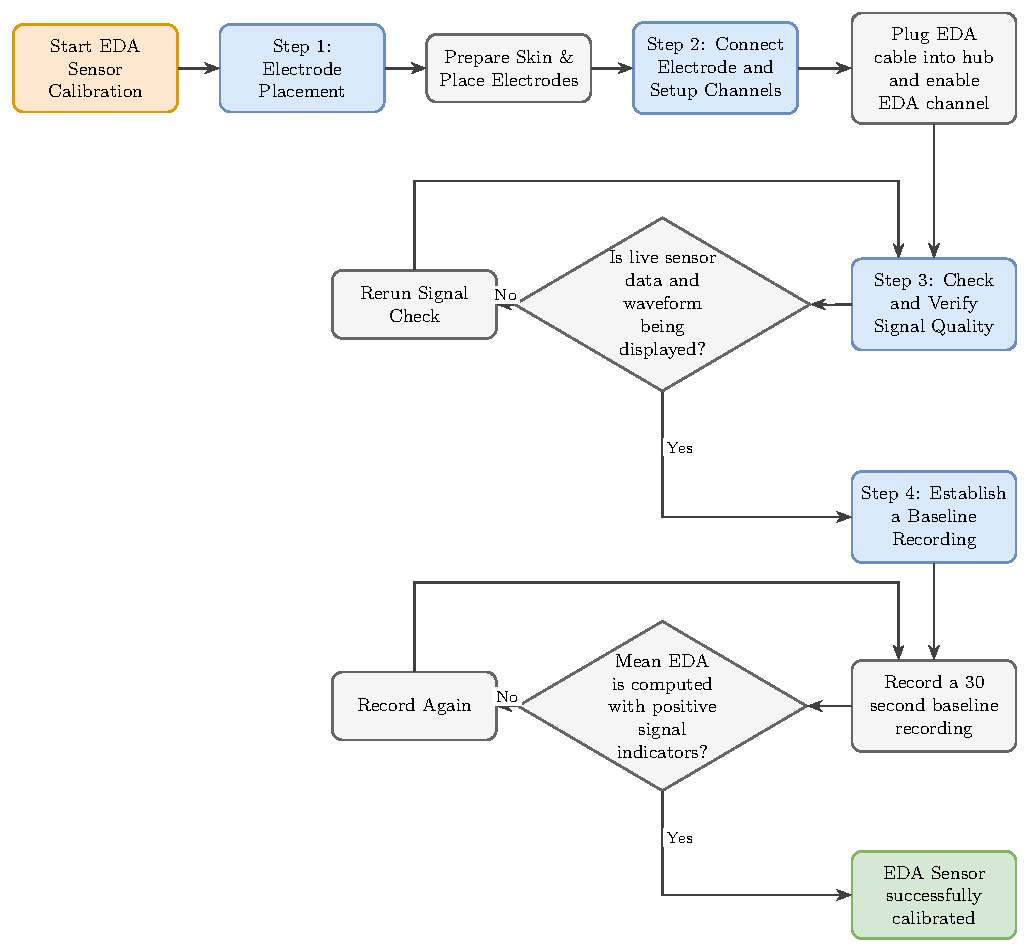
\includegraphics[max width=0.85\linewidth,max totalheight=0.78\textheight]{diagrams/figure-3.20.pdf}\end{center}

\phantomsection\addcontentsline{lof}{figure}{\protect\numberline{3.20}EDA sensor calibration subflow.}%
\textbf{Figure 3.20} EDA sensor calibration subflow. The diagram traces the user\textquotesingle s journey from starting EDA sensor calibration through to a successful calibration.
\end{figure}

\textbf{Step 1: Attach and Place Electrodes:} As seen in Figure 3.21, The flow begins with electrode placement, presented as two grouped checklists, Prepare Skin and Place Electrodes, alongside an anatomical illustration of the correct electrode sites on the palm side of the non-dominant hand, with the red (+) electrode on the index finger and the black (-) electrode on the middle finger, as specified by the manufacturer in the EDA sensor datasheet (PLUX Wireless Biosignals, 2020).

Presenting placement as an explicit checklist rather than as normal continuous text written in paragraphs lets the researcher confirm each precondition in turn (clean skin, dry skin, non-dominant hand, correct finger per electrode), while the illustration removes reliance on memory or an external manual. The "Continue to Connect" action stays disabled until every item is checked, gating progression on correct placement.

\begin{figure}[H]
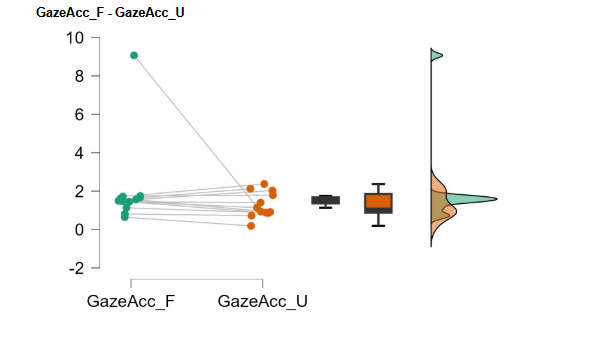
\includegraphics[max width=\linewidth,max totalheight=0.78\textheight]{media/media/image27.png}

\phantomsection\addcontentsline{lof}{figure}{\protect\numberline{3.21}EDA calibration, Step 1: Attach and place electrodes.}%
\textbf{Figure 3.21} EDA calibration, Step 1: Attach and place electrodes. An anatomical illustration shows the correct electrode sites, alongside two checklists for preparing the skin and placing the electrodes. The "Continue to Connect" action stays disabled until every item is checked.
\end{figure}

\textbf{Step 2: Connect Electrodes and Set Up Channels:} The second step guides the researcher through connecting the sensor to the Biosignalsplux hub and configuring the acquisition channel (Figure 3.22). A contextual note explains that the EDA sensor must be connected to an analog input port and is not compatible with reference/ground or digital ports. The accompanying hub diagram marks valid ports with a checkmark and invalid ports with a cross, helping the researcher match the instruction to the physical device. The Connect Hardware and Enable Channel checklists guide the researcher through cable connection and channel setup. The system supports these steps by displaying inline confirmations, such as the resolved channel and detected sensor class, for example: Channel 5, EDA sensor (class 4). Beneath these, a Live Hub Status card reports the connected device address, the EDA channel, and whether a sensor is detected on that channel, giving live confirmation that the configuration entered matches what the hardware actually reports. Progression to signal check is gated on these confirmations.

\begin{figure}[H]
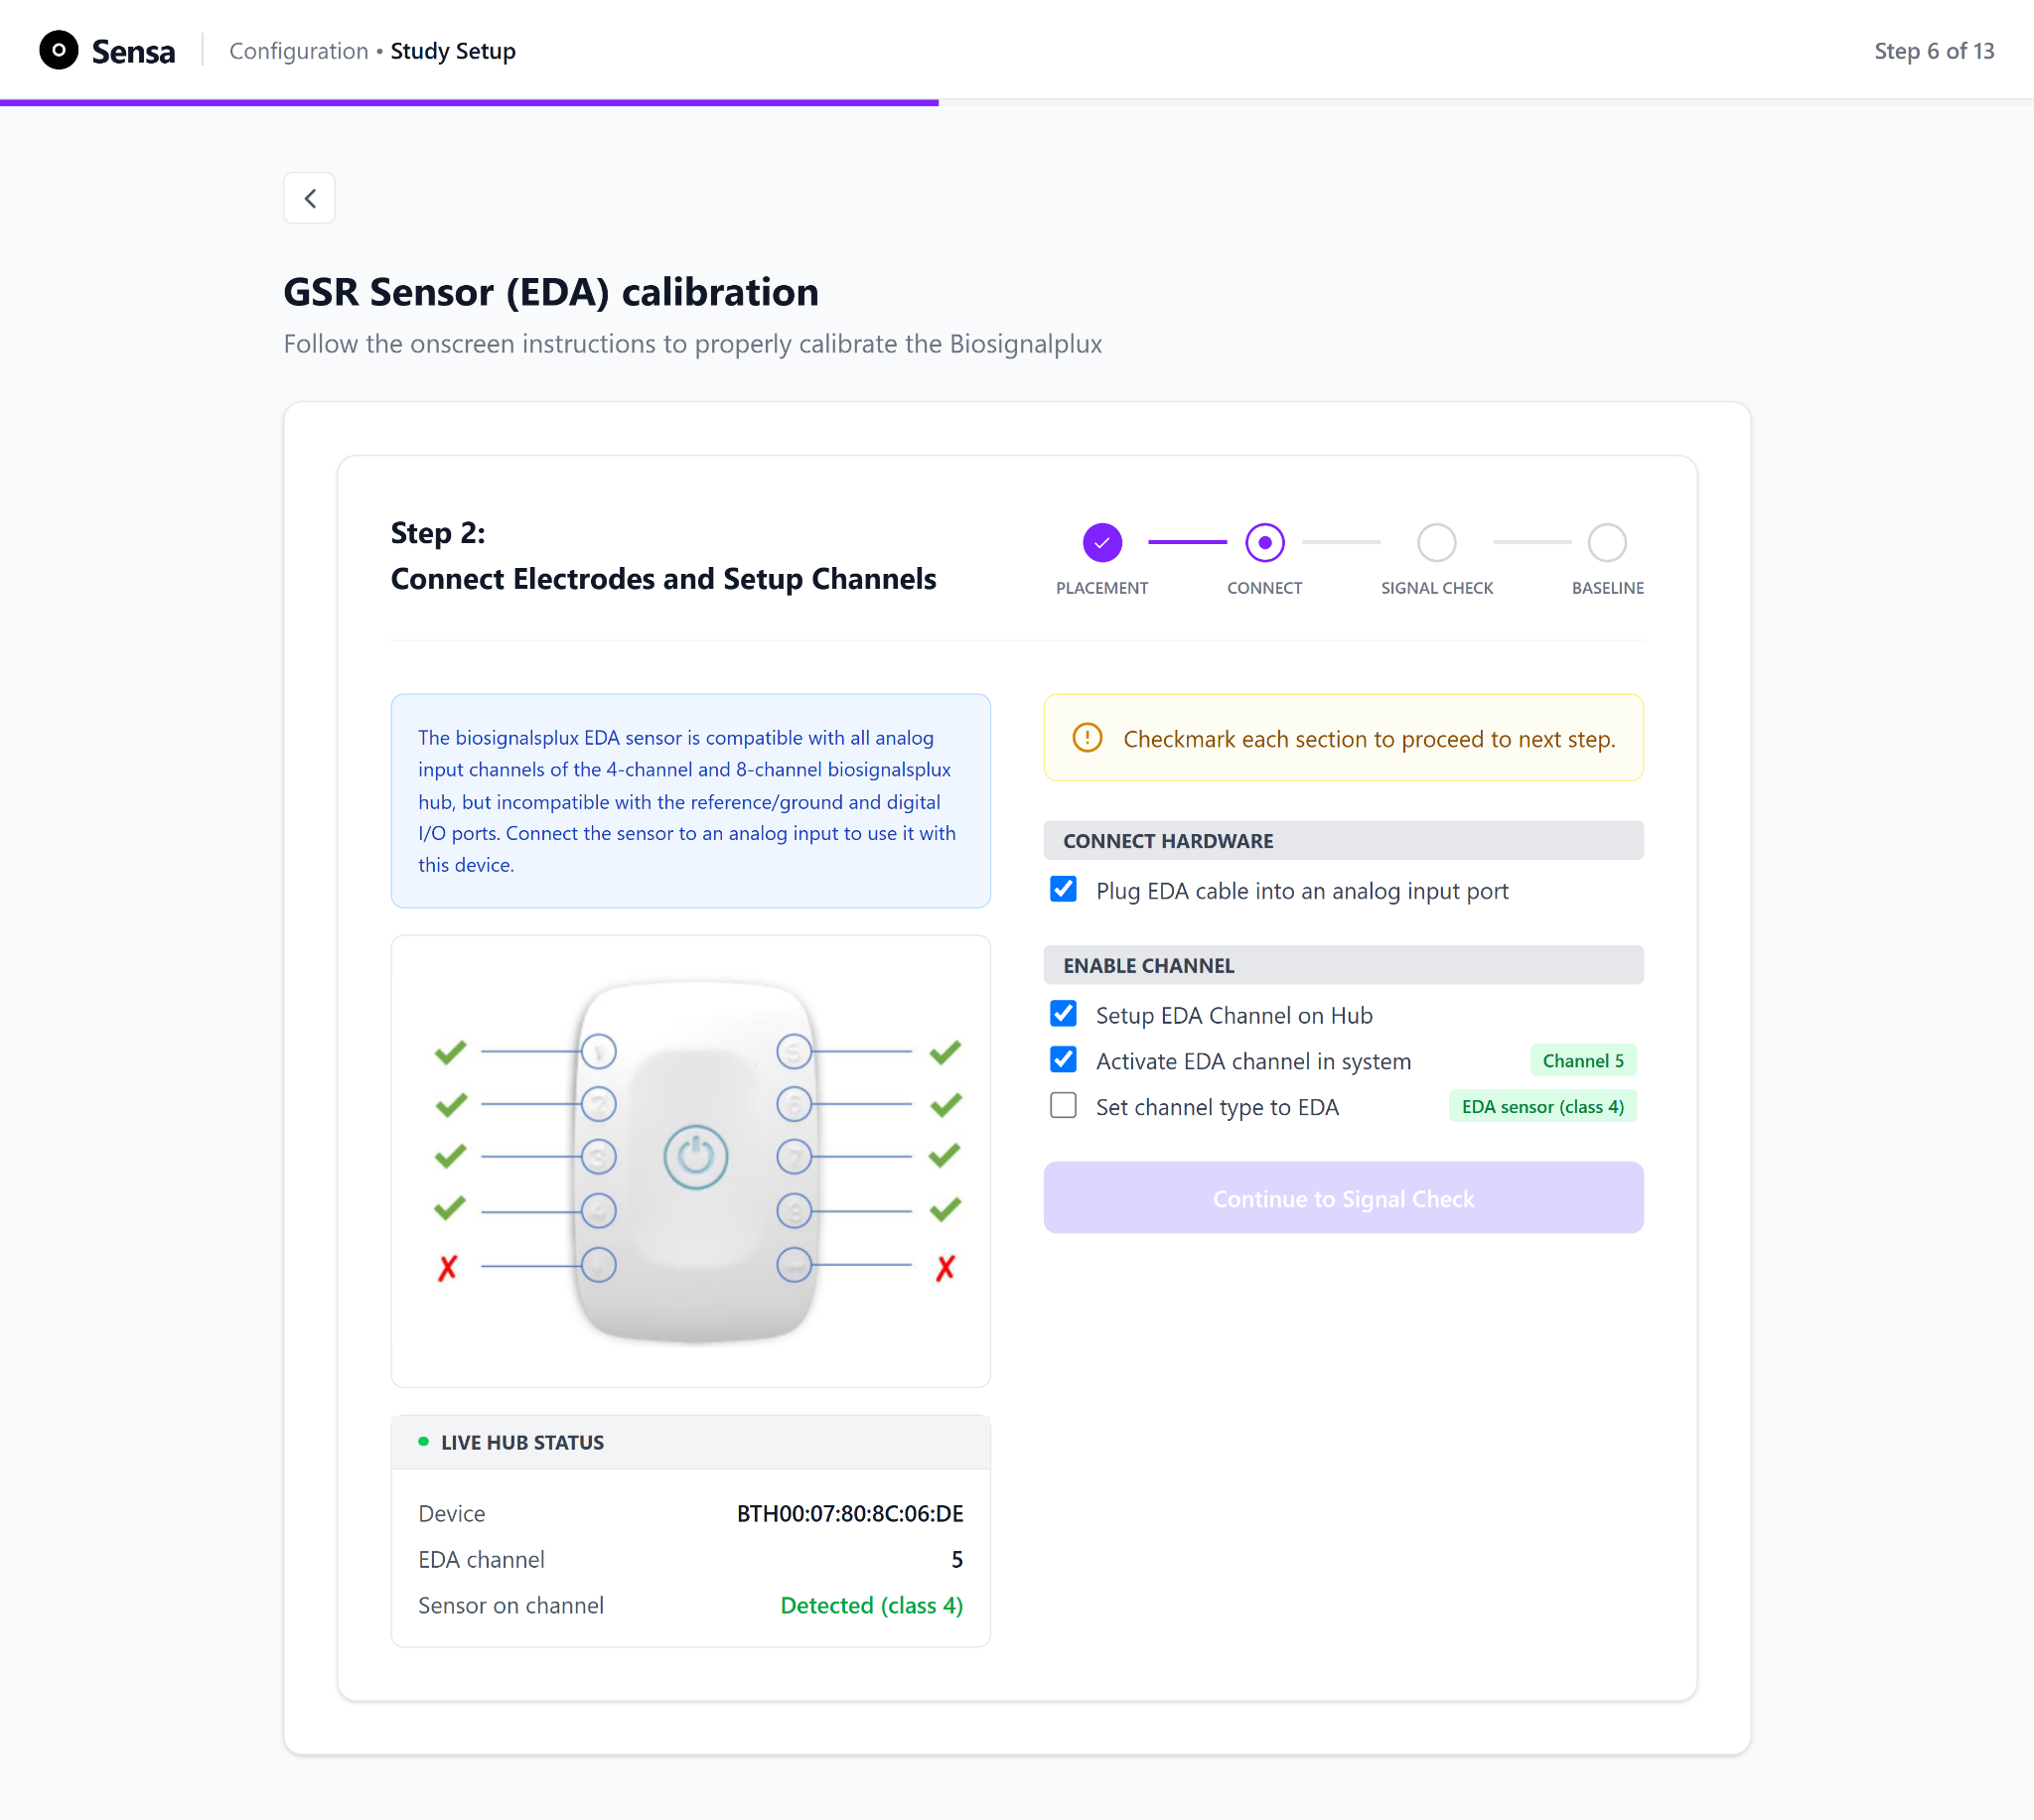
\includegraphics[max width=\linewidth,max totalheight=0.78\textheight]{media/media/image4.png}

\phantomsection\addcontentsline{lof}{figure}{\protect\numberline{3.22}EDA calibration, Step 2: Connect electrodes and set up channels.}%
\textbf{Figure 3.22} EDA calibration, Step 2: Connect electrodes and set up channels. A contextual note explains that the EDA sensor must use an analog port, with a hub diagram marking valid and invalid ports. A Live Hub Status card reports the hub\textquotesingle s connectivity, and the user must check every item to enable the action to proceed to Signal Check.
\end{figure}

\textbf{Step 3: Check and Verify Signal Quality:} Before any data is recorded, the third stage lets the researcher verify that the live signal is usable (Figure 3.23). A live EDA waveform preview plots the incoming signal in real time, with a stream readout beneath it reporting the streaming state, message count, and last sample value, so the researcher can confirm at a glance that data is flowing and that the trace looks physiologically plausible rather than flat or saturated. Alongside it, a Sensor Status card reports two derived indicators. Signal amplitude is the peak-to-peak swing across a rolling sample buffer, and Noise level is the median absolute difference between consecutive samples, expressed as a proportion of that amplitude. Each is colour-coded against fixed thresholds: an acceptable state is shown in green, a borderline state in amber (an unusually low or high amplitude, indicating weak electrode contact or signal saturation respectively), and an unacceptable state in red (a high noise ratio). A "Rerun Signal Check" action allows the researcher to restart the data stream. A short instruction list reminds the participant to sit still, avoid hand movement, and breathe normally during the check.

These thresholds were set empirically during development for this specific sensor and signal range, and are not derived from a published physiological standard. They function as an at-a-glance setup aid for a non-expert operator rather than as a research-grade quality assessment, and this is noted as a limitation of the current design.

The amplitude and noise indicators, their derivation from the live signal, and the thresholds and colour states, were designed and implemented by the author with the assistance of Claude Code (Anthropic). The conversion of the raw signal to microsiemens, which produces the baseline value used as a measure in this study (Chapter 4.5.5), is a separate backend component developed by another contributor.

\begin{figure}[H]
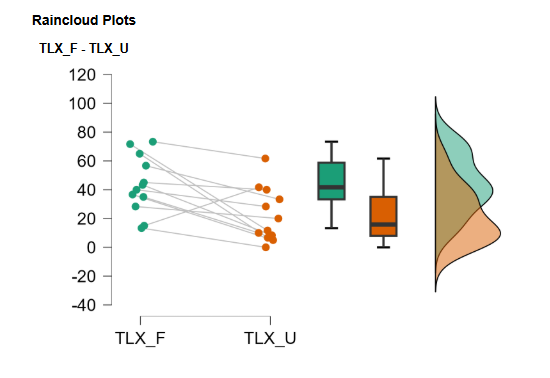
\includegraphics[max width=\linewidth,max totalheight=0.78\textheight]{media/media/image28.png}

\phantomsection\addcontentsline{lof}{figure}{\protect\numberline{3.23}EDA calibration, Step 3: Check and verify signal quality.}%
\textbf{Figure 3.23} EDA calibration, Step 3: Check and verify signal quality. A live waveform preview and a colour-coded Sensor Status card (connection, amplitude, noise) keep the user informed of signal strength and acquisition before a baseline is recorded.
\end{figure}

\textbf{Step 4: Establish a Baseline Recording:} The final stage records a short resting baseline, the participant-specific baseline against which that participant\textquotesingle s session data is later interpreted (Figure 3.24). The user is told that a resting baseline will be recorded and that the participant should be seated and relaxed; the participant is then directed to focus on an on-screen circle and remain still for 30 seconds. On starting the recording, the circle becomes an animated countdown showing the seconds remaining, giving both researcher and participant a continuously visible indication of how much of the baseline task is left and removing the uncertainty of an untimed "hold still" instruction. Throughout the recording, the Sensor Status card continues to report the connection status, amplitude, and noise level in real time. The Baseline field changes from unknown to recording and finally to completed, reporting the mean EDA value in microsiemens. The same colour-coding used for sensor status also flags any deterioration in signal quality during the recording. A focused instruction list (sit still, keep hands relaxed on a flat surface, avoid finger movement, breathe normally, do not talk or shift position until the timer ends) sets the conditions for a clean baseline. On completion, there is a colour coded success/failure message to indicate to the user whether their EDA sensor has been successfully calibrated. If the user is content with the recording, they may choose to export the baseline recording as a .h5 file (a file used to store, organize, and manage massive or complex datasets) or if the user is not satisfied with their recording, they can choose to record a baseline value again (Figure 3.25).

\begin{figure}[H]
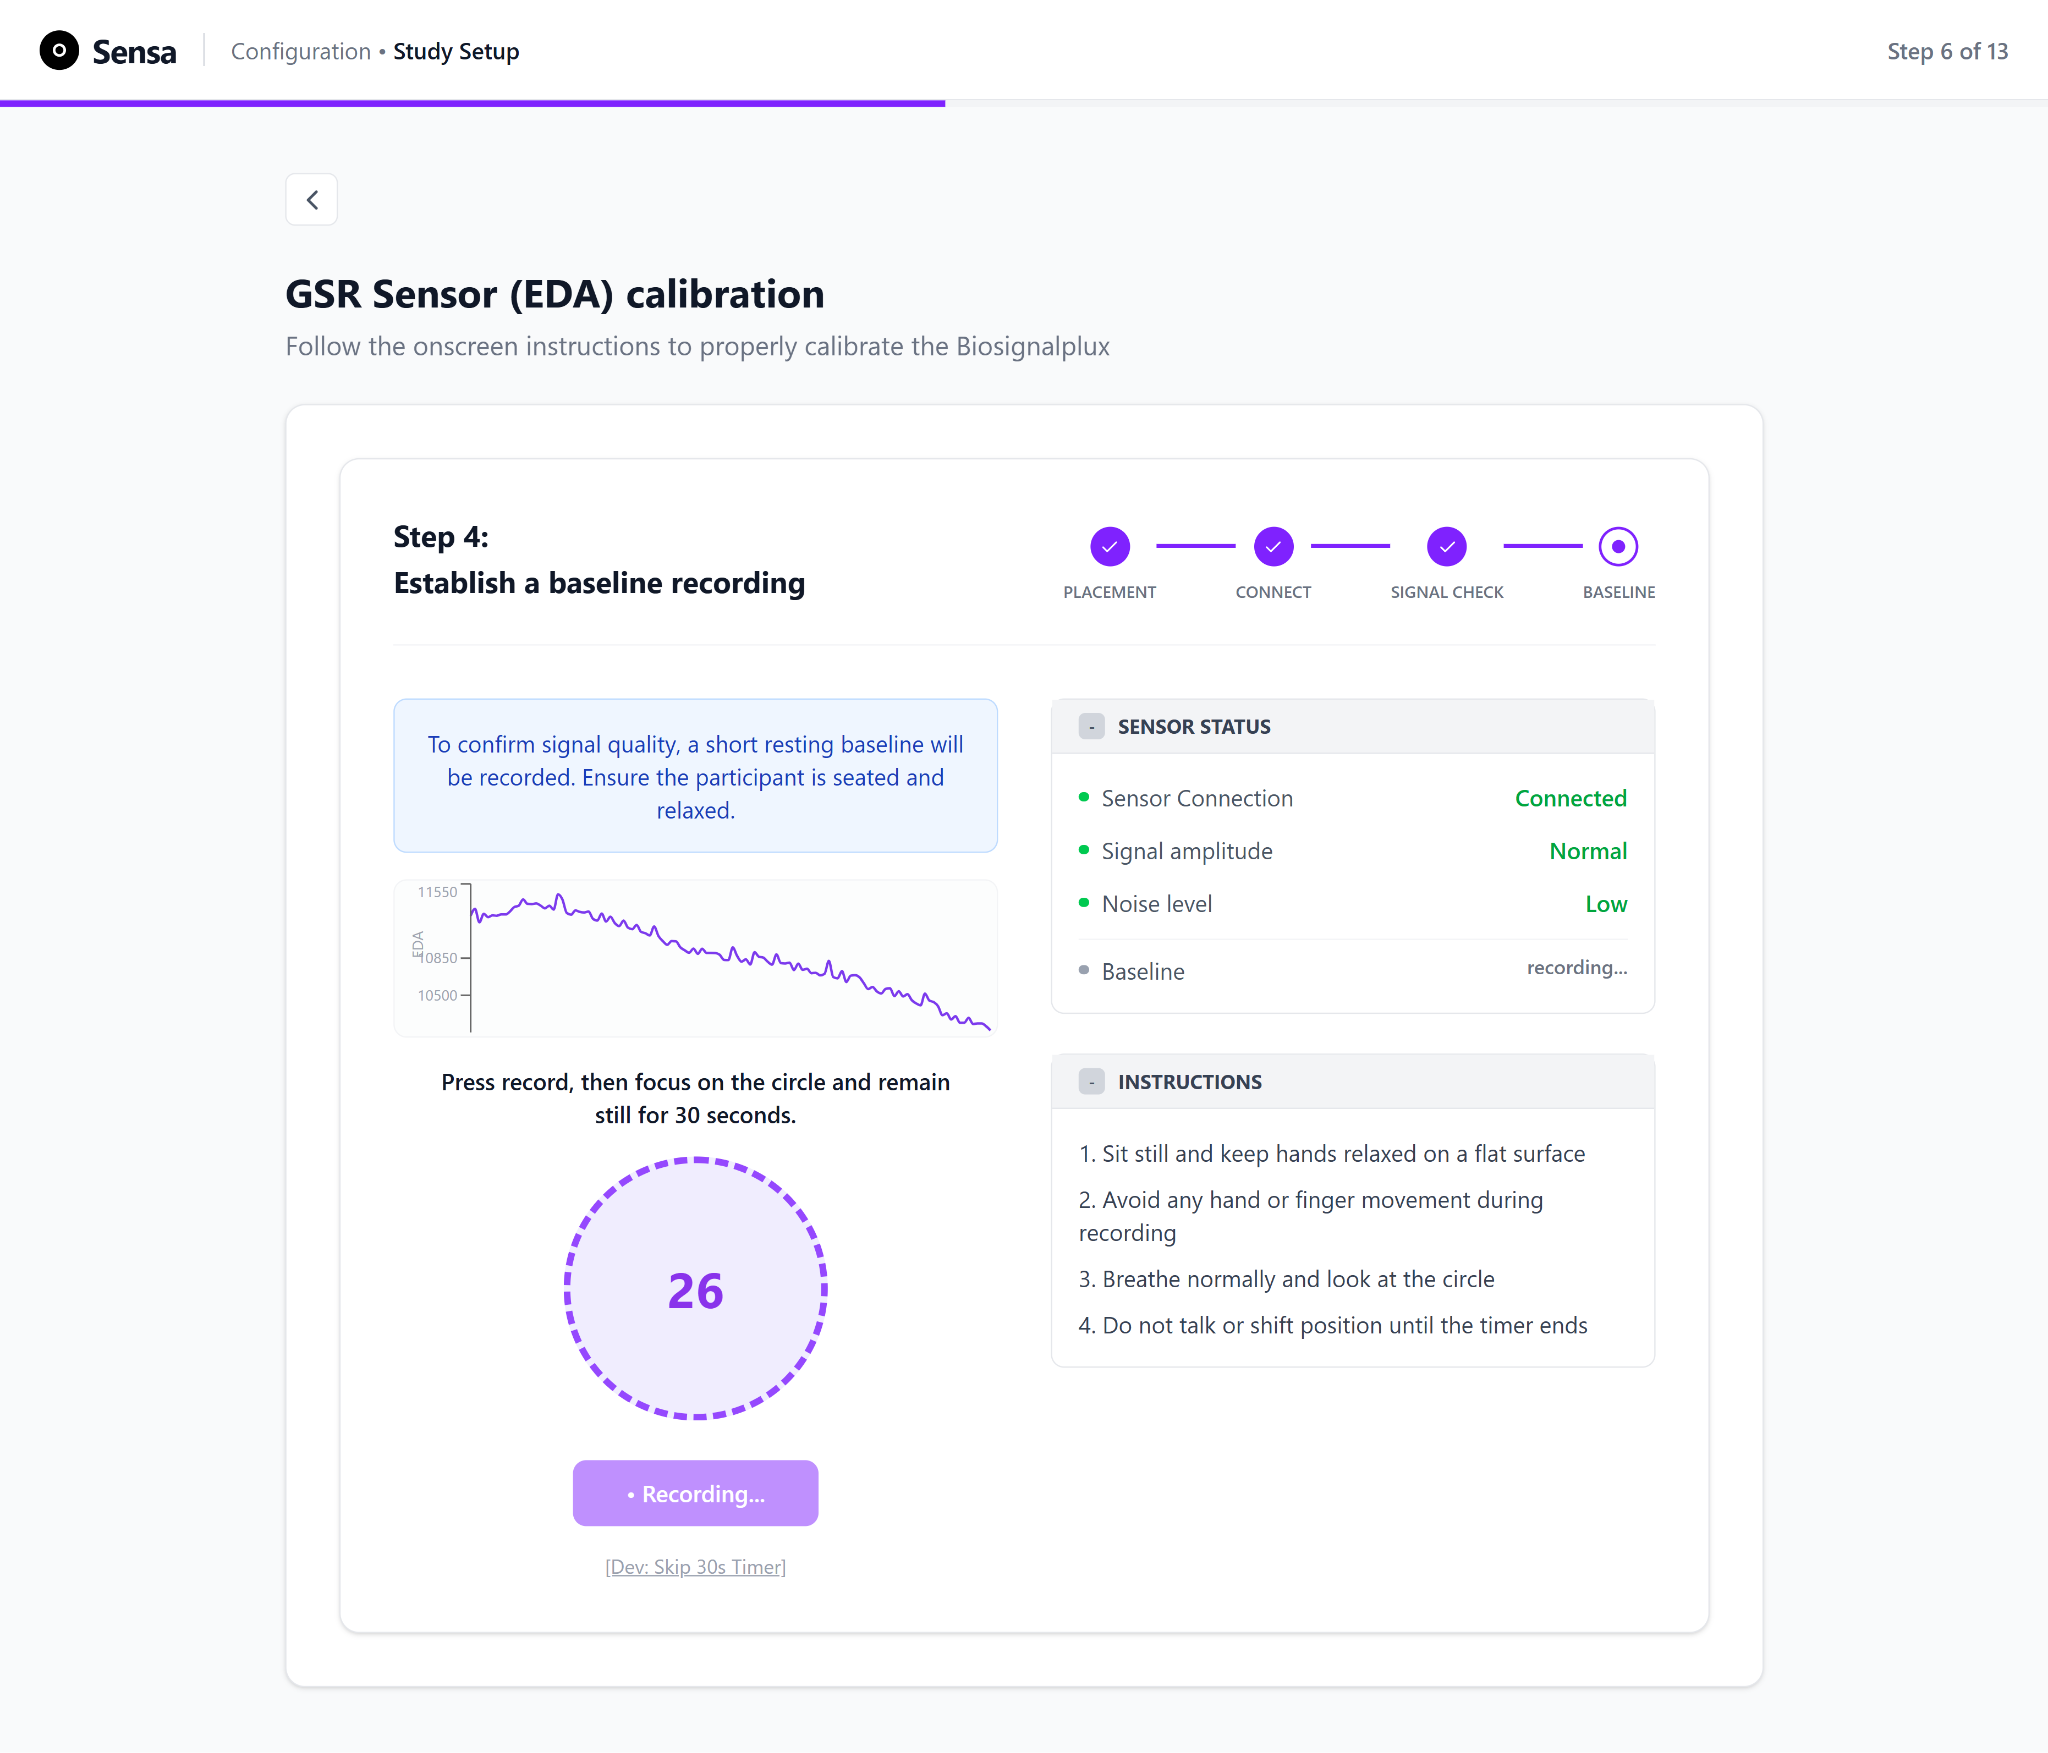
\includegraphics[max width=\linewidth,max totalheight=0.78\textheight]{media/media/image35.png}

\phantomsection\addcontentsline{lof}{figure}{\protect\numberline{3.24}EDA calibration, Step 4: Establish a baseline recording, with recording in progress.}%
\textbf{Figure 3.24} EDA calibration, Step 4: Establish a baseline recording, with recording in progress. A contextual note explains that a short baseline is required. The Sensor Status card reports live signal acquisition and a live waveform confirms data is being recorded, while the instructions ask the user to sit still, breathe normally, and focus on the countdown for 30 seconds.
\end{figure}

Each biosensor calibration follows a similar 4 step process described above, ending with computing a sensor-specific baseline value, which serves as the signal-stability gate before the researcher proceeds to mark the calibration of that sensor as finished.

\begin{figure}[H]

\includegraphics[max width=\linewidth,max totalheight=0.78\textheight]{media/media/image29.png}

\phantomsection\addcontentsline{lof}{figure}{\protect\numberline{3.25}EDA calibration, Step 4: Establish a baseline recording, with recording complete.}%
\textbf{Figure 3.25} EDA calibration, Step 4: Establish a baseline recording, with recording complete. Once the recording finishes, the Baseline (Mean EDA) value is shown alongside a colour-coded success or failure message. The user can then record the baseline again, export the data as a .h5 file, or finish sensor calibration.
\end{figure}

After all sensors have been calibrated, the researcher confirms device readiness by observing calibration overview with success states and proceeding to the Recording phase by clicking on ``Proceed to Recording Data'', as seen in Figure 3.26.

\begin{figure}[H]
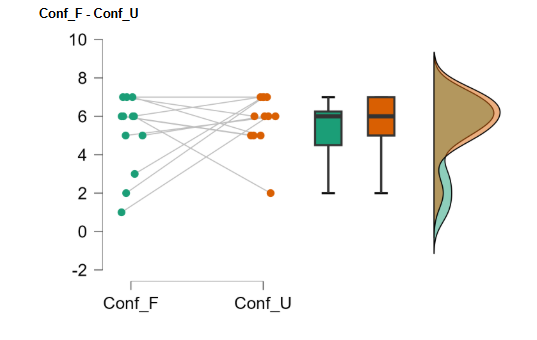
\includegraphics[max width=\linewidth,max totalheight=0.78\textheight]{media/media/image1.png}

\phantomsection\addcontentsline{lof}{figure}{\protect\numberline{3.26}Calibration Overview screen with all sensors in a success state.}%
\textbf{Figure 3.26} Calibration Overview screen with all sensors in a success state. Once every required sensor has been calibrated, the "Proceed to Recording Data" button is enabled.
\end{figure}

\hypertarget{other-modules}{%
\subsection{3.4 Other Modules}\label{other-modules}}

Session recording, data analysis, interpretation, and export modules are part of the broader Sensa platform but are not designed, implemented, or evaluated by the author of this thesis. They are described briefly below to provide system context.

\begin{itemize}
\item
  \emph{Session Recording:} Captures gaze data (fixations, saccades) and biometric data (ECG, EEG, EDA) during stimulus presentation.
\item
  \emph{Data Analysis:} Provides eye-tracking visualizations (heatmaps, fixation maps, AOI metrics) and biometric signal visualizations (EDA peaks, HRV, EEG engagement levels).
\item
  \emph{Interpretation:} Interpret data with help of an interpretation assistant.
\item
  \emph{Export:} Data export in PDF, CSV, and JSON formats.
\end{itemize}

\hypertarget{design-rationale-and-guiding-principles}{%
\subsection{\texorpdfstring{3.5 Design Rationale and Guiding Principles }{3.5 Design Rationale and Guiding Principles }}\label{design-rationale-and-guiding-principles}}

The prototype\textquotesingle s design is informed by Nielsen\textquotesingle s ten usability heuristics (Nielsen, 1994), a widely used framework for evaluating user interface design. These heuristics provide a structured set of design principles, including visibility of system status, match between system and the real world, error prevention, recognition over recall, and consistency. These guide the prototype\textquotesingle s interaction patterns, particularly in long, multi-step procedural tasks such as sensor calibration. The Sensa onboarding and calibration prototype uses Nielsen\textquotesingle s heuristics as the primary framework to guide workflow structure, feedback, and error handling.

Because multi-sensor setup and calibration are procedural tasks with a high likelihood of breakdowns (e.g., missing prerequisites, unclear device state, poor signal quality, and repeated recalibration), the interface emphasizes continuous visibility of system status, recognition over recall, error prevention, and support for recovery.

To reduce cognitive burden during long, multi-step setup processes, the prototype applies \textbf{progressive disclosure} by presenting only the information needed at each stage (e.g., Study Setup \textgreater\textgreater{} Sensor Selection \textgreater\textgreater{} Readiness Check \textgreater\textgreater{} Calibration). Within calibration, complex tasks are decomposed into smaller steps using a stepper-based flow (e.g., Placement \textgreater\textgreater{} Connect \textgreater\textgreater{} Signal Check \textgreater\textgreater{} Baseline), enabling users to focus on one actionable goal at a time.

\hypertarget{application-of-nielsens-usability-heuristics}{%
\subsection{\texorpdfstring{3.6 Application of Nielsen\textquotesingle s Usability Heuristics }{3.6 Application of Nielsen\textquotesingle s Usability Heuristics }}\label{application-of-nielsens-usability-heuristics}}

The following design patterns in the prototype operationalize key Nielsen heuristics:

\begin{itemize}
\item
  \textbf{Visibility of system status:} A persistent step indicator (``Step x of 13'') and progress bar keep users oriented throughout the setup. Mini steppers implemented within each sensor's calibration flow. Calibration states are made explicit through completion feedback (e.g., readiness confirmation) and per-sensor calibration status with a clear option to re-calibrate when needed.
\item
  \textbf{Match between system and the real world:} Calibration steps mirror the natural sequence of lab preparation (environment readiness \textgreater\textgreater{} sensor placement \textgreater\textgreater{} connection \textgreater\textgreater{} signal check \textgreater\textgreater{} baseline), and the interface uses familiar terminology and task framing (e.g., ``Signal Check,'' ``Baseline Recording''), while providing consistent feedback in plain language.
\item
  \textbf{Recognition rather than recall:} Sensor placement is supported through on-screen checklists and diagrams so users are not required to rely on external manuals or memory. Similarly, metric and sensor selection displays show what is selected and summarize it clearly.
\item
  \textbf{Consistency and standards:} Key layout and control patterns remain consistent across the setup flow (e.g., consistent page structure, repeated use of checklist patterns, and consistent placement of primary actions). This reduces learning effort as users move between setup phases and later between sensor calibration modules.
\item
  \textbf{Error prevention and recovery:} Prerequisite gating (e.g., disabled ``Start Sensor Calibration'' until readiness checks are complete) prevents users from entering calibration in an invalid state. Where issues are likely (e.g., signal quality), the interface provides direct instructions (e.g., ``avoid jaw movement,'' ``sit still'') and supports iterative correction through explicit ``re-calibrate'' actions.
\item
  \textbf{Help and documentation (at point of need):} Explanatory microcopy supports decision-making without forcing users to leave the workflow (e.g., ``Why these recommendations?'' and step-level instructions during calibration).
\end{itemize}


\clearpage
\hypertarget{methodology}{%
\section{4. Methodology}\label{methodology}}

This study employed a controlled, within-subjects experimental design to evaluate the onboarding and calibration workflow designed in this thesis. The evaluation focused exclusively on the phases within the author\textquotesingle s individual contribution: study setup, sensor selection, readiness verification, and sensor calibration and validation. Other platform modules, such as recording, analysis, interpretation, and export, were not evaluated, as they were developed by collaborating team members and fall outside the research question, which concerns the design and usability of the onboarding and calibration workflow specifically.

The comparison was made between two workflow conditions: a fragmented baseline and the unified workflow implemented in Sensa. The baseline condition is termed fragmented because the operator must use Tobii Core and OpenSignals as two independent applications with no shared workflow state, no cross-system feedback, and no unified guidance between eye-tracking calibration and biosensor setup. The unified workflow integrates these phases into a single guided interface.

Participants were assessed on five outcome dimensions: setup and calibration time (H1), perceived workload (H2), perceived usability (H3), observable interaction breakdowns (H4), and eye-tracking calibration outcome quality (H5). Each dimension is operationally defined in Chapter 4.5. Data were collected through manual note-taking, screen recording, timestamp logging, standardized questionnaires (NASA-TLX, SUS, and a Likert-scale calibration confidence rating), the eye-tracking validation procedure described in Chapter 4.4.3, and a short post-task open questionnaire. The mean EDA resting baseline was additionally recorded in both conditions and reported descriptively as a comparability check (see Chapter 4.5), not as a scored quality dimension.

\hypertarget{research-design}{%
\subsection{4.1 Research Design}\label{research-design}}

The study used a within-subjects, counterbalanced design in which every participant completed both conditions:

\hypertarget{fragmented-workflow-baseline-condition}{%
\subsubsection{\texorpdfstring{4.1.1 Fragmented Workflow (Baseline Condition): }{4.1.1 Fragmented Workflow (Baseline Condition): }}\label{fragmented-workflow-baseline-condition}}

Participants performed onboarding and calibration using the native software tools of each system separately (\emph{Tobii Core} for eye tracking and \emph{Biosignalsplux OpenSignals} for the EDA sensor). The two systems were operated sequentially and without integration: eye-tracking calibration was completed first in Tobii Core, followed by EDA electrode placement, bluetooth connection, and signal verification in OpenSignals, after which a resting baseline was recorded and the mean EDA value was computed from the exported recording using a provided Python script in Jupyter. No unified interface, shared workflow logic, or cross-system guidance was provided at any stage. Screenshots of each fragmented tool as participants encountered them are provided in Appendix A.

This condition reflected the standard fragmented workflow commonly encountered in multi-sensor research environments, in which researchers must navigate tools with varying interfaces, terminology, and calibration procedures. The eye-tracking calibration step followed the standard operator-led procedure supported by Tobii Core, which presented calibration targets as exploding dots and guided the user with on-screen instructions.

The biosensor setup followed the device connection and signal verification sequence described in the OpenSignals documentation and was consistent with the signal-level validity assessment approach proposed by Van Lier et al. (2020, p. 16).

Participants were given a task description, written by the researcher and provided in Appendix B, and access to the respective software interfaces (Tobii Core for eye tracking and OpenSignals for the EDA sensor), and were expected to follow on-screen software instructions where available. No step-by-step guidance was provided by the researcher during the task.

\hypertarget{unified-workflow-proposed-condition}{%
\subsubsection{\texorpdfstring{4.1.2 Unified Workflow (Proposed Condition): }{4.1.2 Unified Workflow (Proposed Condition): }}\label{unified-workflow-proposed-condition}}

Participants used \emph{\textbf{Sensa\textquotesingle s}} onboarding and calibration module designed in this thesis, which integrates both systems into a single guided interface with structured steps, contextual instructions, readiness checks, calibration guidance, and eye-tracking validation, and which computes the mean EDA value internally.

Because the design was within-subjects, every participant experienced both conditions, and the order was counterbalanced to control for learning and fatigue effects. A simple AB/BA counterbalancing scheme was used: participants were assigned to a condition order in strict alternation, so that the first participant completed the fragmented condition followed by the unified condition, the second completed the unified condition followed by the fragmented condition, and so on. A five-minute break separated the two conditions for each participant. Participants self-administered each condition by following a printed task prompt (Appendix B1 for the fragmented condition, Appendix B2 for the unified condition); the researcher did not provide step-by-step guidance during the task, observing silently and logging interaction breakdowns, think-aloud remarks, and behavioural observations. All sessions were screen-recorded using OBS Studio (OBS Project Contributors, 2026) so that interaction breakdowns and timestamps could be reconfirmed during analysis.

\hypertarget{participants}{%
\subsection{4.2 Participants}\label{participants}}

Twelve participants (N = 12) took part, each completing both conditions and contributing paired observations. Participants were recruited by convenience sampling from the HSRW student body and staff. All twelve reported regular use of a desktop or laptop computer for work or study, satisfying the basic computer-literacy inclusion criterion; no prior experience with Tobii Core, OpenSignals, or biosignal sensors was required.

The sample comprised seven Master\textquotesingle s students, four Bachelor\textquotesingle s students, and one PhD student/research assistant, drawn from a range of disciplines. Usability Engineering was the most represented field, alongside Design and Interaction, Infotronic Systems Engineering, Communication and Information Engineering, Mobility and Logistics, and International Management and Psychology. Most participants were aged 25 to 34 (n = 9), with two aged 18 to 24 and one aged 35 to 44. Five of the twelve participants identified as women while seven identified as men.

Prior experience with the two relevant technologies was recorded through the intake form (Appendix C). Participants who answered yes to either "Have you previously used eye-tracking software or hardware (for example, Tobii eye trackers or similar)?" or "Have you previously placed biosignal electrodes (for example, EEG, EDA/GSR, or ECG sensors) on yourself or another person?" were classified as experienced on that technology. This is reported descriptively, since it was not used for group assignment: every participant completed both conditions, and the counterbalanced order described in Chapter 4.1 controlled for order effects. Five of the twelve participants had previously used eye-tracking hardware or software, and seven had previously placed biosignal electrodes (EEG, EDA/GSR, or ECG) on themselves or another person. Since the experimental design was within-subjects, participants were not split into separate groups; every participant completed both conditions. To control for order effects, each participant was randomly assigned to one of two counterbalanced condition orders (unified-first or fragmented-first).

\Needspace{26\baselineskip}
Table 4.1 summarizes participant characteristics.

\begin{longtable}[]{@{}
  >{\raggedright\arraybackslash}p{(\columnwidth - 4\tabcolsep) * \real{0.4774}}
  >{\raggedright\arraybackslash}p{(\columnwidth - 4\tabcolsep) * \real{0.4397}}
  >{\raggedright\arraybackslash}p{(\columnwidth - 4\tabcolsep) * \real{0.0628}}@{}}
\toprule\noalign{}
\begin{minipage}[t]{\linewidth}\raggedright
\textbf{Characteristic}
\end{minipage} & \begin{minipage}[t]{\linewidth}\raggedright
\textbf{Category}
\end{minipage} & \begin{minipage}[t]{\linewidth}\raggedright
\textbf{n}
\end{minipage} \\
\begin{minipage}[t]{\linewidth}\raggedright
\textbf{Role}
\end{minipage} & \begin{minipage}[t]{\linewidth}\raggedright
Master's Student
\end{minipage} & \begin{minipage}[t]{\linewidth}\raggedright
7
\end{minipage} \\
\begin{minipage}[t]{\linewidth}\raggedright
\end{minipage} & \begin{minipage}[t]{\linewidth}\raggedright
Bachelor\textquotesingle s student
\end{minipage} & \begin{minipage}[t]{\linewidth}\raggedright
4
\end{minipage} \\
\begin{minipage}[t]{\linewidth}\raggedright
\end{minipage} & \begin{minipage}[t]{\linewidth}\raggedright
PhD student / research assistant
\end{minipage} & \begin{minipage}[t]{\linewidth}\raggedright
1
\end{minipage} \\
\begin{minipage}[t]{\linewidth}\raggedright
\textbf{Age}
\end{minipage} & \begin{minipage}[t]{\linewidth}\raggedright
18-24
\end{minipage} & \begin{minipage}[t]{\linewidth}\raggedright
2
\end{minipage} \\
\begin{minipage}[t]{\linewidth}\raggedright
\end{minipage} & \begin{minipage}[t]{\linewidth}\raggedright
25-34
\end{minipage} & \begin{minipage}[t]{\linewidth}\raggedright
9
\end{minipage} \\
\begin{minipage}[t]{\linewidth}\raggedright
\end{minipage} & \begin{minipage}[t]{\linewidth}\raggedright
35-44
\end{minipage} & \begin{minipage}[t]{\linewidth}\raggedright
1
\end{minipage} \\
\begin{minipage}[t]{\linewidth}\raggedright
\textbf{Identified Gender}
\end{minipage} & \begin{minipage}[t]{\linewidth}\raggedright
Male
\end{minipage} & \begin{minipage}[t]{\linewidth}\raggedright
7
\end{minipage} \\
\begin{minipage}[t]{\linewidth}\raggedright
\end{minipage} & \begin{minipage}[t]{\linewidth}\raggedright
Female
\end{minipage} & \begin{minipage}[t]{\linewidth}\raggedright
5
\end{minipage} \\
\begin{minipage}[t]{\linewidth}\raggedright
\textbf{Prior eye-tracking experience}
\end{minipage} & \begin{minipage}[t]{\linewidth}\raggedright
Yes
\end{minipage} & \begin{minipage}[t]{\linewidth}\raggedright
5
\end{minipage} \\
\begin{minipage}[t]{\linewidth}\raggedright
\end{minipage} & \begin{minipage}[t]{\linewidth}\raggedright
No
\end{minipage} & \begin{minipage}[t]{\linewidth}\raggedright
7
\end{minipage} \\
\begin{minipage}[t]{\linewidth}\raggedright
\textbf{Prior biosignal electrode placement}
\end{minipage} & \begin{minipage}[t]{\linewidth}\raggedright
Yes
\end{minipage} & \begin{minipage}[t]{\linewidth}\raggedright
7
\end{minipage} \\
\begin{minipage}[t]{\linewidth}\raggedright
\end{minipage} & \begin{minipage}[t]{\linewidth}\raggedright
No
\end{minipage} & \begin{minipage}[t]{\linewidth}\raggedright
5
\end{minipage} \\
\begin{minipage}[t]{\linewidth}\raggedright
\textbf{Regular computer use}
\end{minipage} & \begin{minipage}[t]{\linewidth}\raggedright
Yes
\end{minipage} & \begin{minipage}[t]{\linewidth}\raggedright
12
\end{minipage} \\
\midrule\noalign{}
\endhead
\bottomrule\noalign{}
\endlastfoot
\end{longtable}

\phantomsection\addcontentsline{lot}{table}{\protect\numberline{4.1}Participant characteristics.}%
\textbf{Table 4.1} Participant characteristics. Summary of the demographic and background characteristics of the twelve participants.

\hypertarget{apparatus-and-materials}{%
\subsection{4.3 Apparatus and Materials}\label{apparatus-and-materials}}

The hardware comprised a Tobii Eye Tracker 4C, a screen-mounted, consumer-grade device operated through the Tobii Eye Tracking Core Software (Tobii AB, 2021), used for eye-tracking calibration, and a Biosignalsplux EDA sensor used for the electrodermal resting baseline. The Sensa setup interface presented eye tracking, EEG, ECG, and EDA as selectable sensors, but only the eye tracker and the EDA sensor were physically connected and measured in this study. EEG and ECG were never connected; they appeared as selectable options to reflect the platform\textquotesingle s intended multimodal scope, and were excluded from measurement to keep the within-subjects session length manageable and to focus the evaluation on two distinct calibration types, a spatial calibration (eye tracking) and a resting-baseline acquisition (EDA).

The software setup differed between conditions. In the fragmented condition, the Tobii Core Eye Tracking Software (Tobii AB, 2021) handled eye-tracking calibration for the consumer 4C; OpenSignals (PLUX Wireless Biosignals S.A., 2026) served as the recording software for the Biosignalsplux EDA sensor, handling bluetooth connection, real-time signal display, and export of the recording for offline analysis; and a pre-made Python script, run in Jupyter, computed the mean EDA value in microsiemens from the exported recording using a fixed transfer function (PLUX Wireless Biosignals, 2020, p. 2). In the unified condition, the Sensa prototype (described in Chapter 3) computed the mean EDA value internally using the same transfer function. OBS Studio was used for screen recording and timestamp capture in both conditions. A single laptop ran all software, and the same machine and the same EDA conversion were used across both conditions, so that any difference in outcomes was attributable to the workflow rather than to the underlying hardware or computation. All testing was conducted under identical environmental conditions (same lab, lighting, and equipment setup) at the Usability Lab, Rhine-Waal University, Kamp Lintfort.

The study materials consisted of a participant information sheet (Appendix D), an informed consent form (Appendix E), the task prompts (Appendix B1 for the fragmented condition and Appendix B2 for the unified condition), per-condition observation and breakdown log sheets (Appendix F), the post-task open-response questionnaire (Appendix G), and post-task objective questionnaire comprising of System Usability Scale (SUS), the Raw NASA-TLX, and the calibration confidence rating (Appendix H).

\hypertarget{experimental-procedure}{%
\subsection{4.4 Experimental Procedure}\label{experimental-procedure}}

\textbf{Session structure (common to both conditions)}

On arrival, the participant was welcomed, given the participant information sheet (Appendix D), and briefed on the purpose of the study, including a short, non-evaluative introduction to eye tracking and biometric sensor technology. The participant then read and signed the informed consent form (Appendix E).

The participant was then asked to complete the first condition according to their assigned counterbalanced order, self-administering the task from a printed prompt (Appendix B1 for the fragmented condition, Appendix B2 for the unified condition). Throughout each condition, the experimenter observed silently and logged interaction breakdowns, think-aloud remarks, and behavioural observations, while OBS Studio recorded the screen and timestamps for post-session reconfirmation of breakdowns and timing. The experimenter did not provide step-by-step guidance during the task, intervening only to clarify the task or in the event of a critical breakdown.\\
\strut \\
At the end of each condition, the participants were instructed to fill out a post-task open-response questionnaire (Appendix G) and the post-task objective questionnaire (Appendix H), followed by a 5 minute break. Both were administered immediately after each condition, before the participant proceeded, so that responses referred to the workflow just experienced rather than to a retrospective comparison of the two.

The post-task open-response questionnaire administered as a Google Form, covered four targeted areas, each explored through open-ended written questions rather than rating scales: ease of use (which steps felt straightforward or difficult, and why), clarity of guidance (whether instructions and feedback were sufficient to complete the task without confusion), calibration confidence (whether the participant would trust the data collected from this session), and perceived workflow quality (how the participant perceived the overall structure and flow of the process they used).

The post-task objective questionnaire comprised the SUS, the Raw NASA-TLX, and a calibration confidence rating (Likert 1-7). The SUS comprises the ten standard items rated on a five-point agreement scale, yielding a composite score from 0 to 100, and addressed H3 (that the unified workflow is rated more usable than the fragmented workflow). The Raw NASA-TLX records the six standard dimensions (mental demand, physical demand, temporal demand, performance, effort, and frustration), each on a 0 to 10 scale, and addresses H2 (that the unified workflow imposes lower cognitive workload). Physical demand was included for completeness but was not a primary dimension of interest given the task context. The calibration confidence rating was a single seven-point item (1 = not at all confident, 7 = completely confident): "How confident are you that the sensors were correctly calibrated and that the system was ready to record reliable data?", with an optional free-text follow-up in which participants could explain the reason for their confidence rating, for example naming a specific step that left them unsure. This provided qualitative context for the numeric confidence score. It supplemented H3 by capturing perceived calibration outcome quality from the participant\textquotesingle s perspective, which SUS alone does not address.

\hypertarget{fragmented-condition-procedure}{%
\subsubsection{4.4.1 Fragmented condition procedure}\label{fragmented-condition-procedure}}

In the fragmented condition the participant used the native software tools of each system separately, Tobii Core for the eye tracker and Biosignalsplux OpenSignals for the EDA sensor, with no unified guidance between them. The printed task prompt (Appendix B1) describes a fictional researcher scenario and the sequential steps to complete. The workflow proceeds in three sequential phases:

\textbf{Study documentation:} The participant records the study parameters manually in a provided Google Docs template (Appendix I), reflecting the absence of a unified study-creation interface. The parameters recorded are the same as those Sensa\textquotesingle s Study Setup flow captures in the unified condition: study name, study goal, interface type, test environment, sensors and metrics to use, number of participants, and study objectives. This ensures the documentation step is able to be compared across conditions and that time spent on study documentation is included consistently in the setup-time dependent variable for both conditions.

\textbf{Eye-tracking calibration:} The participant opens Tobii Core, positions themselves at the recommended viewing distance of approximately 60 cm from the screen-mounted eye tracker, and completes the calibration procedure with themselves as the calibration subject. The participant may refer to the printed extract from the Tobii Eye Tracking software user guide (Appendix J) if needed. They then validate the calibration using Tobii Core\textquotesingle s native gaze-trace visualization, which provides a qualitative visual check of tracking quality but reports no numeric accuracy or precision values. Recalibration is repeated if the participant judges the result unsatisfactory, based on their own judgement of the qualitative gaze-trace visualization, which is the only quality information Tobii Core exposes. The numeric calibration-quality data for this condition are not collected here; they are obtained afterwards through Sensa\textquotesingle s validation grid, administered as a separate measurement step (see Chapter 4.4.3).

\textbf{EDA sensor setup}: The participant places the EDA electrode using a printed reference sheet (Appendix K), ensures that the Biosignalsplux hub is connected via bluetooth, opens OpenSignals, and verifies signal presence by visual inspection of the live waveform. Signal verification in the baseline condition involves the participant visually confirming, on OpenSignals\textquotesingle{} live-waveform display, that the EDA channel shows: (a) a waveform that is present and oscillating (not flat-lined); and (b) no obvious clipping (no flat-topped peaks at the display boundaries); following an instruction on the task sheet to confirm whether the EDA waveform was flat or oscillating. A waveform that was present and oscillating (not flat-lined) and free of obvious clipping (no flat-topped peaks at the display boundaries) was treated as an acceptable signal. No quantitative threshold was applied at this step; this visual confirmation of waveform presence and the absence of obvious artefacts is the operational definition of signal verification for the baseline condition, consistent with the standard OpenSignals workflow it reflects (PLUX Wireless Biosignals S.A., 2026).

The participant then records a 30-second resting baseline and computes the mean EDA value (in microsiemens) from the exported recording using a provided Python script in Jupyter Lab, reporting the resulting value.

\hypertarget{unified-condition-procedure}{%
\subsubsection{4.4.2 Unified condition procedure}\label{unified-condition-procedure}}

In the unified condition, participants used the Sensa prototype, which integrates both systems into a single guided onboarding and calibration sequence. The printed task prompt (Appendix B2) describes the same fictional researcher scenario used in the fragmented condition. The workflow proceeds through the platform\textquotesingle s guided sequence:

\textbf{Study setup:} The participant defines the study goal, interface type, test environment, and available hardware through the Sensa onboarding flow (described in detail in Chapter 3.3.1, Figures 3.3 to 3.5), and selects the sensors and metrics from the supported options. As in the fragmented condition, eye tracking, EEG, ECG, and EDA are all selectable, but only the eye tracker and the EDA sensor are connected and calibrated in this study (see Chapter 4.3).

\textbf{Readiness check:} The participant confirms all readiness checklist items before proceeding to calibration.

\textbf{Sensor calibration:} The participant calibrates each connected sensor using Sensa\textquotesingle s guided calibration flow, which provides on-screen instructions, visual diagrams, and step-by-step feedback for each device. For the eye tracker (Tobii Eye Tracker 4C), this includes track-box positioning feedback, the guided calibration, and Sensa\textquotesingle s five-point validation, which the participant runs in-flow, sees the numeric result of, and may act on by recalibrating before proceeding (see Chapter 4.4.3). For the EDA sensor (Biosignalsplux), this includes electrode placement, signal-quality verification, and recording a 30-second resting baseline, with the mean EDA value computed internally by Sensa and reported by the participant.

A task was marked complete, in either condition, when the participant had calibrated both the eye tracker and the EDA sensor and notified the experimenter that the system was ready to begin recording. Task success required that the participant is confident in the eye-tracker calibration and has successfully obtained and reported the mean EDA value.

\hypertarget{eye-tracking-calibration-quality-check}{%
\subsubsection{4.4.3 Eye-Tracking Calibration Quality Check}\label{eye-tracking-calibration-quality-check}}

Following calibration, a post-calibration validation procedure was used to quantify gaze accuracy, precision, and valid data yield. A validation step was necessary because empirically measured accuracy and precision frequently diverge from manufacturer-stated specifications and must be reported independently (Dalrymple et al., 2018, p. 9). The measurement instrument was Sensa\textquotesingle s five-point validation grid, and was applied in both conditions so that numerical calibration quality could be recorded by the same tool throughout. Sensa does not perform the gaze calibration itself: in both conditions the gaze model is built by Tobii, and Sensa only measures its result. This is what allows Sensa\textquotesingle s validation layer to act as a neutral scorer rather than as part of the workflow being compared.

In the unified condition, validation is a part of the participant\textquotesingle s guided flow. After calibrating, the participant runs Sensa\textquotesingle s five-point validation, sees the result, and may recalibrate within the workflow before declaring the system ready.

In the fragmented condition, the participant validates their own calibration during the task using Tobii Core\textquotesingle s native gaze-trace visualization, which provides a qualitative visual check but reports no numeric accuracy or precision. The numeric calibration-quality data for this condition are collected separately: after the participant has completed the fragmented task and finished the post-task objective and open-ended questionnaires, the experimenter administers Sensa\textquotesingle s five-point validation grid as a measurement step only, without recalibrating Tobii Core. This validation step is performed only after the fragmented task has been completed. Therefore, it does not influence the measured setup time, breakdown counts, or questionnaire responses in the fragmented condition. At the same time, it allows the study to collect numeric accuracy, precision, and data-yield values using the same validation method as in the unified Sensa condition.

The validation grid presents five targets located at the four corners and the centre of the usable display area. For each target, binocular gaze samples are collected and used to calculate accuracy, precision, and valid data yield. Accuracy and precision are reported in degrees of visual angle, using the participant\textquotesingle s measured viewing distance rather than a fixed field-of-view assumption. A target is classified as passing if its accuracy remains within the configurable threshold, which is set to 3.0 degrees for the Tobii 4C, providing a small margin relative to the realistic upper accuracy range of approximately 2.5 degrees reported for consumer-grade trackers (Mikalef et al., 2023, p. 4). The extracted calibration-quality measures include mean accuracy, mean precision, valid data yield, per-target accuracy, first-pass calibration success, and recalibration count. These measures are formally defined as dependent variables in Chapter 4.5.

Since the same Sensa validation procedure is used to score both conditions, any systematic bias in its accuracy calculation is applied consistently across the unified and fragmented workflows. This makes the resulting calibration-quality measures suitable for comparing the two conditions, even if the absolute values should be interpreted with caution. The counterbalanced study order described in Chapter 4.1 further reduces the risk that order effects influence the measurement. However, the reported accuracy and precision values should not be treated as externally validated ground-truth measurements. The validation procedure is custom-built and has not been validated against a reference-grade eye-tracking validation system. Therefore, the values are interpreted as instrument-relative measures. This limitation is acknowledged in Chapter 4.7. It does not undermine the relative comparison between workflows, which is the basis for evaluating H5.

\hypertarget{dependent-variables-metrics}{%
\subsection{4.5 Dependent Variables (Metrics)}\label{dependent-variables-metrics}}

Dependent variables were calculated from three data sources, depending on the variable class. (1) Timing and breakdown metrics (H1, H4) were extracted from the session observation sheets and screen recordings (OBS Studio) through post-hoc annotation, with timestamps taken from the recording rather than from a live stopwatch. (2) Subjective measures, like NASA-TLX, SUS, and the calibration confidence rating (H2, H3) were computed from the standardized post-task questionnaires, scored according to each instrument\textquotesingle s published procedure. (3) Eye-tracking calibration quality metrics (H5) were computed from Sensa\textquotesingle s five-point validation grid (Chapter 3.3.4), which was applied in both conditions. In addition, the mean EDA resting baseline was computed from the 30-second recording using the shared transfer function and reported descriptively (see below). All dependent variables were calculated identically across the two conditions to ensure comparability, and because the design was within-subjects, each participant contributed a paired value per measure.

\hypertarget{efficiency-measures-relates-to-h1}{%
\subsubsection{4.5.1 Efficiency Measures (relates to H1)}\label{efficiency-measures-relates-to-h1}}

\begin{itemize}
\item
  \textbf{Setup Time (sec):} The total elapsed time to reach a recording-ready state, measured from the start of study setup to the point at which both sensors were calibrated and the participant declared readiness. Timestamps were read from the OBS recording.
\item
  \textbf{Calibration Time (sec):} The portion of setup time spent specifically on sensor calibration. In the fragmented condition this was the sum of the eye-tracker calibration duration (in Tobii Core) and the EDA setup-and-baseline duration (in OpenSignals). In the unified condition it was the elapsed time from the start of Sensa\textquotesingle s sensor-calibration step to calibration completion.
\end{itemize}

\hypertarget{subjective-user-experience-measures-relates-to-h2-h3}{%
\subsubsection{4.5.2 Subjective User Experience Measures (relates to H2 \& H3)}\label{subjective-user-experience-measures-relates-to-h2-h3}}

\begin{itemize}
\item
  \textbf{SUS Score (0--100):} overall perceived usability (See Appendix H Section 1).
\item
  \textbf{Raw NASA-TLX (0--10):} six workload dimensions (mental, physical, temporal demand, performance, effort, frustration) (See Appendix H Section 2).
\item
  \textbf{Calibration confidence rating (1-7 Likert-scale)}: perceived reliability and user confidence (See Appendix H Section 3).
\end{itemize}

\hypertarget{interaction-breakdown-metrics-relates-to-h4}{%
\subsubsection{\texorpdfstring{4.5.3 Interaction Breakdown Metrics (relates to H4): }{4.5.3 Interaction Breakdown Metrics (relates to H4): }}\label{interaction-breakdown-metrics-relates-to-h4}}

Interaction breakdowns were operationally defined as observable events that interrupted or delayed task progression. They were included as dependent variables because time-on-task alone does not reveal where or why a workflow creates friction; breakdown counts give a more granular picture of where the fragmented and unified workflows diverged. Each breakdown event was counted and logged by the experimenter during the session. A \textbf{total breakdown count per participant} per condition was calculated by summing the following event types:

\begin{itemize}
\item
  \textbf{Repeated calibration attempts (Eye Tracker):} Counted each time a participant restarted the eye-tracking calibration after an unsatisfactory result, beyond the first attempt. This captures whether the workflow provided sufficient guidance to achieve calibration success on the first attempt, or whether unclear feedback or inadequate instruction forced a retry.
\item
  \textbf{Repeated baseline recordings (EDA):} Counted each time a participant had to restart or repeat the 30-second EDA baseline after an incomplete or unusable first attempt (for example due to movement, low user confidence in recording, a dropped signal, or stopping early). This captures whether the workflow provided adequate confidence and guidance to complete the recording successfully.
\item
  \textbf{Incorrect sequence execution:} Counted each time a participant performed a workflow step out of the intended order (for example starting a recording or a later step before completing a required earlier one). This captures whether the workflow structure was intuitive enough to follow without deviation, or whether the absence of unified guidance led to procedural errors
\item
  \textbf{Hesitation periods (more than 5 seconds of inactivity)}: Counted each time a participant paused for more than 5 seconds of inactivity while uncertain how to proceed. This captures moments where the interface failed to provide sufficient guidance or feedback at that point in the workflow.
\item
  \textbf{Requests for clarification}: Counted each time a participant asked the experimenter for help because on-screen instructions were insufficient. This captures gaps in the workflow\textquotesingle s self-sufficiency, where the participant could not proceed on the interface alone.
\end{itemize}

\hypertarget{calibration-outcome-quality-relates-to-h5}{%
\subsubsection{4.5.4 Calibration Outcome Quality (relates to H5)}\label{calibration-outcome-quality-relates-to-h5}}

Calibration outcome quality was evaluated for the eye-tracking modality only, using the metrics produced by Sensa\textquotesingle s five-point validation grid (Chapter 3.3.4), computed identically in both conditions. Accuracy, precision, and valid data yield are spatial gaze-quality metrics specific to eye tracking and have no direct equivalent for EDA, whose readiness is instead a matter of signal quality and a resting baseline. The EDA baseline is therefore not scored as a calibration-quality dimension but reported descriptively as a comparability check (Chapter 4.5.5).

\begin{itemize}
\item
  \textbf{Mean gaze accuracy (degrees of visual angle):} the systematic offset between target and mean recorded gaze, averaged across valid targets.
\item
  \textbf{Mean gaze precision (degrees of visual angle):} the random dispersion of gaze samples about their own mean.
\item
  \textbf{Valid data yield (\%):} the proportion of collected samples containing a valid binocular gaze estimate.
\item
  \textbf{Per-target accuracy (degrees):} the individual accuracy at each of the five targets.
\item
  \textbf{First-pass calibration success (binary):} whether the calibration the participant committed to passed Sensa\textquotesingle s validation on first measurement.
\item
  \textbf{Recalibration count:} the number of recalibration attempts during the task.
\end{itemize}

\hypertarget{eda-baseline-comparability-check-not-a-scored-h5-dimension}{%
\subsubsection{4.5.5 EDA baseline (comparability check, not a scored H5 dimension)}\label{eda-baseline-comparability-check-not-a-scored-h5-dimension}}

A 30-second resting EDA baseline was recorded in both conditions to check whether participants had comparable physiological starting levels. The mean EDA value (microsiemens) was computed from the recording using the same transfer function in both conditions and reported descriptively (mean and standard deviation). It was not treated as a calibration-quality measure. Since the conversion and hardware were identical across conditions, the workflow could not mechanically alter this value; any between-condition difference would reflect participant arousal state rather than calibration quality.

\Needspace{27\baselineskip}
All dependent variables summarized in Table 4.2 were compared within participants across the two conditions (fragmented vs unified).

\begin{longtable}[]{@{}
  >{\raggedright\arraybackslash}p{(\columnwidth - 8\tabcolsep) * \real{0.1748}}
  >{\raggedright\arraybackslash}p{(\columnwidth - 8\tabcolsep) * \real{0.3166}}
  >{\raggedright\arraybackslash}p{(\columnwidth - 8\tabcolsep) * \real{0.1235}}
  >{\raggedright\arraybackslash}p{(\columnwidth - 8\tabcolsep) * \real{0.1510}}
  >{\raggedright\arraybackslash}p{(\columnwidth - 8\tabcolsep) * \real{0.2142}}@{}}
\toprule\noalign{}
\begin{minipage}[t]{\linewidth}\raggedright
\textbf{Construct}
\end{minipage} & \begin{minipage}[t]{\linewidth}\raggedright
\textbf{Dependent variable}
\end{minipage} & \begin{minipage}[t]{\linewidth}\raggedright
\textbf{Unit/scale}
\end{minipage} & \begin{minipage}[t]{\linewidth}\raggedright
\textbf{Hypothesis}
\end{minipage} & \begin{minipage}[t]{\linewidth}\raggedright
\textbf{Source}
\end{minipage} \\
\begin{minipage}[t]{\linewidth}\raggedright
Efficiency
\end{minipage} & \begin{minipage}[t]{\linewidth}\raggedright
Setup time
\end{minipage} & \begin{minipage}[t]{\linewidth}\raggedright
seconds
\end{minipage} & \begin{minipage}[t]{\linewidth}\raggedright
H1
\end{minipage} & \begin{minipage}[t]{\linewidth}\raggedright
OBS Recording
\end{minipage} \\
\begin{minipage}[t]{\linewidth}\raggedright
Efficiency
\end{minipage} & \begin{minipage}[t]{\linewidth}\raggedright
Calibration time
\end{minipage} & \begin{minipage}[t]{\linewidth}\raggedright
seconds
\end{minipage} & \begin{minipage}[t]{\linewidth}\raggedright
H1
\end{minipage} & \begin{minipage}[t]{\linewidth}\raggedright
OBS Recording
\end{minipage} \\
\begin{minipage}[t]{\linewidth}\raggedright
Workload
\end{minipage} & \begin{minipage}[t]{\linewidth}\raggedright
Raw NASA-TLX (6 dimensions)
\end{minipage} & \begin{minipage}[t]{\linewidth}\raggedright
0-10 each
\end{minipage} & \begin{minipage}[t]{\linewidth}\raggedright
H2
\end{minipage} & \begin{minipage}[t]{\linewidth}\raggedright
Questionnaire
\end{minipage} \\
\begin{minipage}[t]{\linewidth}\raggedright
Usability
\end{minipage} & \begin{minipage}[t]{\linewidth}\raggedright
SUS score
\end{minipage} & \begin{minipage}[t]{\linewidth}\raggedright
0-100
\end{minipage} & \begin{minipage}[t]{\linewidth}\raggedright
H3
\end{minipage} & \begin{minipage}[t]{\linewidth}\raggedright
Questionnaire
\end{minipage} \\
\begin{minipage}[t]{\linewidth}\raggedright
Confidence
\end{minipage} & \begin{minipage}[t]{\linewidth}\raggedright
Calibration confidence
\end{minipage} & \begin{minipage}[t]{\linewidth}\raggedright
1-7
\end{minipage} & \begin{minipage}[t]{\linewidth}\raggedright
H3
\end{minipage} & \begin{minipage}[t]{\linewidth}\raggedright
Questionnaire
\end{minipage} \\
\begin{minipage}[t]{\linewidth}\raggedright
Breakdowns
\end{minipage} & \begin{minipage}[t]{\linewidth}\raggedright
Total breakdown count (5 event types)
\end{minipage} & \begin{minipage}[t]{\linewidth}\raggedright
count
\end{minipage} & \begin{minipage}[t]{\linewidth}\raggedright
H4
\end{minipage} & \begin{minipage}[t]{\linewidth}\raggedright
Observation + recording
\end{minipage} \\
\begin{minipage}[t]{\linewidth}\raggedright
Calibration quality
\end{minipage} & \begin{minipage}[t]{\linewidth}\raggedright
Mean gaze accuracy
\end{minipage} & \begin{minipage}[t]{\linewidth}\raggedright
degrees
\end{minipage} & \begin{minipage}[t]{\linewidth}\raggedright
H5
\end{minipage} & \begin{minipage}[t]{\linewidth}\raggedright
Sensa 5-point grid
\end{minipage} \\
\begin{minipage}[t]{\linewidth}\raggedright
Calibration quality
\end{minipage} & \begin{minipage}[t]{\linewidth}\raggedright
Mean gaze precision
\end{minipage} & \begin{minipage}[t]{\linewidth}\raggedright
degrees
\end{minipage} & \begin{minipage}[t]{\linewidth}\raggedright
H5
\end{minipage} & \begin{minipage}[t]{\linewidth}\raggedright
Sensa 5-point grid
\end{minipage} \\
\begin{minipage}[t]{\linewidth}\raggedright
Calibration quality
\end{minipage} & \begin{minipage}[t]{\linewidth}\raggedright
Valid data yield
\end{minipage} & \begin{minipage}[t]{\linewidth}\raggedright
\%
\end{minipage} & \begin{minipage}[t]{\linewidth}\raggedright
H5
\end{minipage} & \begin{minipage}[t]{\linewidth}\raggedright
Sensa 5-point grid
\end{minipage} \\
\begin{minipage}[t]{\linewidth}\raggedright
Calibration quality
\end{minipage} & \begin{minipage}[t]{\linewidth}\raggedright
Per-target accuracy
\end{minipage} & \begin{minipage}[t]{\linewidth}\raggedright
degrees
\end{minipage} & \begin{minipage}[t]{\linewidth}\raggedright
H5
\end{minipage} & \begin{minipage}[t]{\linewidth}\raggedright
Sensa 5-point grid
\end{minipage} \\
\begin{minipage}[t]{\linewidth}\raggedright
Calibration quality
\end{minipage} & \begin{minipage}[t]{\linewidth}\raggedright
First-pass calibration success
\end{minipage} & \begin{minipage}[t]{\linewidth}\raggedright
binary
\end{minipage} & \begin{minipage}[t]{\linewidth}\raggedright
H5
\end{minipage} & \begin{minipage}[t]{\linewidth}\raggedright
Sensa 5-point grid
\end{minipage} \\
\begin{minipage}[t]{\linewidth}\raggedright
Calibration quality
\end{minipage} & \begin{minipage}[t]{\linewidth}\raggedright
Recalibration count
\end{minipage} & \begin{minipage}[t]{\linewidth}\raggedright
count
\end{minipage} & \begin{minipage}[t]{\linewidth}\raggedright
H5
\end{minipage} & \begin{minipage}[t]{\linewidth}\raggedright
Observation + Sensa grid
\end{minipage} \\
\begin{minipage}[t]{\linewidth}\raggedright
Comparability
\end{minipage} & \begin{minipage}[t]{\linewidth}\raggedright
Mean EDA baseline
\end{minipage} & \begin{minipage}[t]{\linewidth}\raggedright
microsiemens
\end{minipage} & \begin{minipage}[t]{\linewidth}\raggedright
descriptive only
\end{minipage} & \begin{minipage}[t]{\linewidth}\raggedright
descriptive only
\end{minipage} \\
\midrule\noalign{}
\endhead
\bottomrule\noalign{}
\endlastfoot
\end{longtable}

\phantomsection\addcontentsline{lot}{table}{\protect\numberline{4.2}Dependent variables.}%
\textbf{Table 4.2} Dependent variables. Summary of all dependent variables, the hypothesis they map onto, and the sources used to evaluate them.

\hypertarget{data-analysis}{%
\subsection{\texorpdfstring{4.6 Data Analysis }{4.6 Data Analysis }}\label{data-analysis}}

The study generated two complementary data types. Quantitative data were derived from the measurements collected in each experimental condition, including system-recorded performance and interaction measures, questionnaire scores, and eye-tracking quality metrics. These measures produced one value per participant for each condition. Quantitative differences between conditions were analysed using paired statistical tests based on each participant's results in both conditions. Quantitative analyses were carried out in JASP (JASP Team, 2026), with an alpha level of .05 and two-tailed tests throughout. Despite the directional hypotheses, two-tailed tests were retained. This was done to ensure consistency across the hypothesis set and to allow detection of effects in the opposite direction. This was particularly important for the calibration-quality measures in H5, because any deterioration in data quality would have been both theoretically significant and practically concerning.

One constraint shapes how every statistical result in this thesis should be read: the small sample size limits statistical power. With twelve participants, the paired comparisons can reliably detect only large effects (approximately dz = 0.9 at 80\% power, α = .05). A large difference between the workflows is therefore likely to reach significance, but a smaller, real difference may not, and this risk is greatest for the subjective measures, where any effect is expected to be more modest. The consequences of this are twofold. First, a non-significant result must not be read as evidence that the two workflows do not differ, or that they are equivalent, on that measure; it may simply mean the study could not detect the difference. Second, effect sizes and their confidence intervals carry particular weight in this study, because they show the estimated size and direction of a difference regardless of whether it crosses a significance threshold. For this reason, an effect size and 95\% confidence interval are reported alongside every test, and the subjective measures are interpreted primarily through them.

\hypertarget{quantitative-analysis}{%
\subsubsection{4.6.1 Quantitative Analysis}\label{quantitative-analysis}}

The quantitative analysis followed a predefined sequence covering test selection, effect sizes, the binary outcome, multiple-comparison correction, and the interpretation of H5 and the EDA check

\hypertarget{step-1-normality-screening-and-the-choice-of-test}{%
\paragraph{4.6.1.1 Normality screening and the choice of test}\label{step-1-normality-screening-and-the-choice-of-test}}

For each continuous or interval dependent variable defined in Chapter 4.5, the within-participant difference scores were first screened for normality using the Shapiro--Wilk test. Normally distributed differences were analysed using a paired-samples t-test; otherwise, the Wilcoxon signed-rank test was used. The difference scores for setup time, calibration time, SUS, NASA-TLX, calibration confidence, interaction breakdowns, valid-data yield, and the EDA baseline were approximately normally distributed. These measures were therefore analysed using paired-samples t-tests. The differences for gaze accuracy and gaze precision departed from normality and were compared with the Wilcoxon signed-rank test, which does not assume normally distributed differences. Because of the small sample size, exact p-values were calculated where possible instead of relying on approximations intended for larger samples.

\hypertarget{step-2-reporting-the-effect-sizes}{%
\paragraph{4.6.1.2 Reporting the effect sizes}\label{step-2-reporting-the-effect-sizes}}

An effect size and its 95\% confidence interval are reported for each test: Cohen's (d\_z) for paired-samples t-tests and matched-pairs rank-biserial correlation for Wilcoxon signed-rank tests. These estimates are considered alongside the significance tests because, with only twelve participants, a binary decision based on the corrected significance threshold provides limited information about the magnitude and uncertainty of an effect. Accordingly, large estimated effects that do not meet the family-wise threshold, such as those for calibration time and gaze precision, are interpreted as potentially meaningful differences that remain statistically uncertain because of the small sample and conservative correction.

\hypertarget{step-3-analysing-the-binary-outcome-using-mcnemars-test}{%
\paragraph{4.6.1.3 Analysing the binary outcome using McNemar's test}\label{step-3-analysing-the-binary-outcome-using-mcnemars-test}}

One measure, first-pass calibration success, could not be analysed with the tests above because it is not a score but a paired yes-or-no outcome: in each condition, a participant\textquotesingle s calibration either passed validation on the first attempt or it did not. The standard test for this situation is McNemar\textquotesingle s test. The test considers only participants whose outcome differed between conditions and examines whether more participants changed from failure to success than from success to failure. Because only a small number of participants showed such a change, the corresponding counts are reported alongside the test result to make the underlying pattern transparent.

\Needspace{24\baselineskip}
\hypertarget{step-4-controlling-for-multiple-comparisons}{%
\paragraph{4.6.1.4 Controlling for multiple comparisons}\label{step-4-controlling-for-multiple-comparisons}}

A separate Bonferroni correction was applied to the tests belonging to each hypothesis. Tests of different constructs, such as setup time, workload, usability, interaction breakdowns, and calibration quality, were not combined into one correction family because they address different research questions. Applying one correction across all tests would therefore be unnecessarily strict and would reduce the likelihood of detecting genuine effects. Table 4.3 summarizes the resulting families and their adjusted thresholds.

\begin{longtable}[]{@{}
  >{\raggedright\arraybackslash}p{(\columnwidth - 8\tabcolsep) * \real{0.1045}}
  >{\raggedright\arraybackslash}p{(\columnwidth - 8\tabcolsep) * \real{0.1722}}
  >{\raggedright\arraybackslash}p{(\columnwidth - 8\tabcolsep) * \real{0.4919}}
  >{\raggedright\arraybackslash}p{(\columnwidth - 8\tabcolsep) * \real{0.0627}}
  >{\raggedright\arraybackslash}p{(\columnwidth - 8\tabcolsep) * \real{0.1488}}@{}}
\toprule\noalign{}
\begin{minipage}[t]{\linewidth}\raggedright
\textbf{Hypothesis}
\end{minipage} & \begin{minipage}[t]{\linewidth}\raggedright
\textbf{Construct}
\end{minipage} & \begin{minipage}[t]{\linewidth}\raggedright
\textbf{Measures in family}
\end{minipage} & \begin{minipage}[t]{\linewidth}\raggedright
\textbf{Tests}
\end{minipage} & \begin{minipage}[t]{\linewidth}\raggedright
\textbf{Adjusted α}
\end{minipage} \\
\begin{minipage}[t]{\linewidth}\raggedright
H1
\end{minipage} & \begin{minipage}[t]{\linewidth}\raggedright
Efficiency
\end{minipage} & \begin{minipage}[t]{\linewidth}\raggedright
Setup time; calibration time
\end{minipage} & \begin{minipage}[t]{\linewidth}\raggedright
2
\end{minipage} & \begin{minipage}[t]{\linewidth}\raggedright
.025
\end{minipage} \\
\begin{minipage}[t]{\linewidth}\raggedright
H2
\end{minipage} & \begin{minipage}[t]{\linewidth}\raggedright
Workload
\end{minipage} & \begin{minipage}[t]{\linewidth}\raggedright
NASA-TLX
\end{minipage} & \begin{minipage}[t]{\linewidth}\raggedright
1
\end{minipage} & \begin{minipage}[t]{\linewidth}\raggedright
.05
\end{minipage} \\
\begin{minipage}[t]{\linewidth}\raggedright
H3
\end{minipage} & \begin{minipage}[t]{\linewidth}\raggedright
Usability
\end{minipage} & \begin{minipage}[t]{\linewidth}\raggedright
SUS
\end{minipage} & \begin{minipage}[t]{\linewidth}\raggedright
1
\end{minipage} & \begin{minipage}[t]{\linewidth}\raggedright
.05
\end{minipage} \\
\begin{minipage}[t]{\linewidth}\raggedright
H4
\end{minipage} & \begin{minipage}[t]{\linewidth}\raggedright
Breakdowns
\end{minipage} & \begin{minipage}[t]{\linewidth}\raggedright
Total interaction breakdowns
\end{minipage} & \begin{minipage}[t]{\linewidth}\raggedright
1
\end{minipage} & \begin{minipage}[t]{\linewidth}\raggedright
.05
\end{minipage} \\
\begin{minipage}[t]{\linewidth}\raggedright
H5
\end{minipage} & \begin{minipage}[t]{\linewidth}\raggedright
Calibration quality
\end{minipage} & \begin{minipage}[t]{\linewidth}\raggedright
Gaze accuracy; gaze precision; valid data yield; first-pass success
\end{minipage} & \begin{minipage}[t]{\linewidth}\raggedright
4
\end{minipage} & \begin{minipage}[t]{\linewidth}\raggedright
.0125
\end{minipage} \\
\begin{minipage}[t]{\linewidth}\raggedright
-
\end{minipage} & \begin{minipage}[t]{\linewidth}\raggedright
Secondary / check
\end{minipage} & \begin{minipage}[t]{\linewidth}\raggedright
Calibration confidence; EDA baseline
\end{minipage} & \begin{minipage}[t]{\linewidth}\raggedright
-
\end{minipage} & \begin{minipage}[t]{\linewidth}\raggedright
Descriptive only
\end{minipage} \\
\midrule\noalign{}
\endhead
\bottomrule\noalign{}
\endlastfoot
\end{longtable}

\phantomsection\addcontentsline{lot}{table}{\protect\numberline{4.3}Hypothesis families for the Bonferroni correction.}%
\textbf{Table 4.3} Hypothesis families for the Bonferroni correction. The confirmatory tests in each family and the per-family adjusted significance threshold.

Calibration confidence was included as a secondary outcome, while the mean EDA baseline was used to assess comparability between conditions. Because neither measure was linked to a predefined hypothesis, both were analysed descriptively and excluded from the multiple-comparison correction applied to the confirmatory tests.

\hypertarget{the-interpretive-stance-on-h5}{%
\paragraph{4.6.1.5 The interpretive stance on H5}\label{the-interpretive-stance-on-h5}}

H5 concerns whether calibration quality differs between the two workflows rather than predicting that either workflow will perform better. Because both conditions use the same Tobii Core calibration engine and Sensa only evaluates the resulting calibration, gaze accuracy and valid data yield were expected to be similar by design. Similar results on these measures are therefore interpreted as consistent with this expectation, but not as evidence of statistical equivalence.

Establishing equivalence would require a formal procedure, such as two one-sided tests, with an adequately powered sample. With only twelve participants, this study cannot support such a claim. The H5 outcomes are therefore interpreted based on the direction, magnitude, and confidence interval of the observed differences rather than on statistical significance alone. This distinction is important because gaze precision showed a substantial difference between conditions, although it did not meet the corrected significance threshold. Treating that result as evidence of equivalence would therefore be misleading.

First-pass calibration success is the H5 outcome most likely to be influenced by the workflow itself and is analysed using McNemar's test, as described above

\hypertarget{the-eda-comparability-check}{%
\paragraph{4.6.1.6 The EDA comparability check}\label{the-eda-comparability-check}}

Finally, mean EDA is included only to assess comparability between conditions and is not treated as a study outcome. The mean and standard deviation are reported for each condition to verify that the resting baseline signal and its conversion to microsiemens were consistent across workflows. Any accompanying paired test is interpreted solely as an acquisition and conversion check, not as a test of a study hypothesis.

\hypertarget{qualitative-analysis}{%
\subsubsection{4.6.2 Qualitative Analysis}\label{qualitative-analysis}}

The qualitative data consisted of the written open-ended post-task responses from the online questionnaire (Appendix G), supported by the observation and breakdown log sheets kept for each condition. Together these provided 24 response sets, one per participant in each of the two conditions, drawn from three sources: the five open-ended post-task questions, the open-ended item accompanying the confidence rating, and the researcher\textquotesingle s observation notes. These data were analysed using reflexive thematic analysis, following Braun and Clarke (2006, 2019).

\hypertarget{coding-approach}{%
\paragraph{\texorpdfstring{4.6.2.1 Coding approach }{4.6.2.1 Coding approach }}\label{coding-approach}}

The written responses and observation notes were coded using a hybrid deductive-inductive approach.

Before the analysis, an initial set of twelve deductive codes was defined from the study\textquotesingle s research focus, as shown in Appendix L, Table L.1. These were derived from three sources. The first was the study\textquotesingle s interaction-breakdown categories, which gave codes for uncertainty about task state, needing help or external reference, sequence or step errors, and repeated calibration or baseline recording (D1 to D4). The second being the study\textquotesingle s usability constructs, which gave codes for ease of use, complexity or overwhelm, calibration confidence, first-time difficulty and learnability, and integration versus tool-switching (D5 to D7, D9, D10). The third were the Nielsen usability heuristics applied in the system design, which gave codes for feedback and visibility of system status, instructions at the point of need, and error prevention and recovery (D8, D11, D12). Together these gave twelve deductive codes, used to identify whether participants\textquotesingle{} responses and observed problems related to the issues the study was designed to examine.

During the analysis, eighteen additional inductive codes were developed directly from the participants\textquotesingle{} responses and the observation notes, as seen in Table L.2. These captured experiences not covered by the initial frame, including reassurance drawn from visible feedback, confusion regarding bluetooth connectivity, anxiety caused by visible readings that looked wrong, uncertainty about sensor placement, the effort of switching between disconnected tools, and the effect of growing familiarity across the two sessions. The deductive and inductive codes together formed a working codebook of thirty codes, reproduced in full in Appendix L.

\hypertarget{analytic-procedure}{%
\paragraph{4.6.2.2 Analytic procedure}\label{analytic-procedure}}

The analysis followed Braun and Clarke's six-phase process (2006). Familiarisation involved repeatedly reading the 24 condition-specific response sets and their accompanying observation notes. During coding, each meaningful segment was assigned to one or more of the thirty codes, allowing responses that reflected several experiences to receive multiple codes.

The codes were then examined for broader patterns and grouped into candidate themes. These themes were reviewed against the coded extracts and the dataset as a whole, with codes merged, reassigned, or retained where necessary. One candidate theme concerning familiarity and condition order was retained as an interpretive theme because it reflected the possible influence of the study procedure rather than a direct experience of either workflow.

This process produced five final themes: confidence grounded in system feedback; the burden of coordinating fragmented tools; guidance from the system; the limits of guidance; and familiarity and order effects. The resulting thematic account is presented in Cahapter 5.2. Appendix L documents the coded extracts, the thirty codes, and their consolidation into the five themes.

\hypertarget{coder-and-reflexivity}{%
\paragraph{4.6.2.3 Coder and reflexivity}\label{coder-and-reflexivity}}

The coding and thematic analysis were carried out by the author, consistent with the single-experimenter design of the study, and the author made all interpretive decisions. An AI assistant (Claude) was used to support the process by helping to organize and document the codes and to surface candidate groupings for the author to evaluate; all codes, themes, and interpretations were reviewed and determined by the author. In keeping with the reflexive, rather than coding-reliability, tradition of thematic analysis, the emphasis is on the transparency of the author\textquotesingle s interpretation, evidenced by the full coding in Appendix L, rather than on inter-coder agreement statistics.

As the designer of the unified onboarding and calibration workflow, the author was not a neutral observer but had a vested interest in the system under evaluation. This dual role therefore required explicit reflexive consideration, particularly because it created a risk of interpreting participants' accounts more favourably towards the unified workflow. To manage the risk of interpreting the findings too favourably, the analysis systematically retained evidence that both supported and challenged the expected benefits of the unified workflow. This does not eliminate the author's potential bias, because coding and theme development still involve interpretive judgement. However, retaining contradictory and negative cases reduces the risk of selectively focusing on evidence that confirms the system's advantages. Accordingly, limitations such as ambiguity in sensor placement, unclear EDA values, and instances in which visible feedback reduced rather than increased confidence were included in the coding and reflected in the final themes. The complete coding in Appendix L provides an audit trail through which readers can assess whether favourable and unfavourable evidence were considered consistently.

\hypertarget{integration-with-the-quantitative-findings}{%
\paragraph{4.6.2.4 Integration with the quantitative findings}\label{integration-with-the-quantitative-findings}}

The interaction breakdowns sit across both strands of the analysis: they were counted per condition as a quantitative dependent variable and, at the same time, categorized by type to feed the thematic analysis. This dual role is intentional since it allows the qualitative account to explain the quantitative pattern rather than sit alongside it. More generally, the qualitative themes are used to contextualise the quantitative results, for example to explain why one workflow produced more breakdowns or why calibration confidence did not differ on average, giving an integrated mixed-methods account rather than two parallel sets of findings.

\hypertarget{validity-and-reliability}{%
\subsection{4.7 Validity and Reliability}\label{validity-and-reliability}}

The study\textquotesingle s validity is supported by its within-subjects design, in which each participant completed both workflow conditions and therefore served as their own control. Hardware, task structure, measurement procedure, and setting were kept as consistent as possible, so that the main difference between conditions was the workflow itself. This chapter discusses the main threats to internal validity, external validity, construct validity, and reliability, and how the design addressed them.

\hypertarget{internal-validity}{%
\subsubsection{4.7.1 Internal Validity}\label{internal-validity}}

The design\textquotesingle s main internal-validity strength is that it is within-subjects: every participant completed both conditions and served as their own control, which removes individual differences such as technical background, general speed, and sensor familiarity from the comparison. In a small sample (N = 12) these differences are the dominant confound, and a between-groups design of this size could not have controlled them.

The principal cost of a within-subjects design is order and carryover effects. Condition order was counterbalanced across participants (Chapter 4.1), and a five-minute break between conditions reduced fatigue and carryover. Beyond order, the two conditions were held identical on everything except the workflow: the same task structure, laboratory, lighting, and equipment, a single laptop running all software, and the same signal processing in both arms (Chapters 4.3 to 4.5). Given that the apparatus and the computation were kept constant, any difference in outcomes is attributable to the workflow rather than to the hardware or signal processing. The calibration-quality comparison is protected in the same way: gaze estimation was performed by the Tobii Core engine and scored by the same validation instrument in both conditions, so neither can be an artefact of one arm alone (Chapters 4.4.3 and 4.6).

Two threats remain and are acknowledged rather than removed. Since both conditions used the same category of task, familiarity with the task content can carry over between them. Counterbalancing distributes this across the two orders but does not eliminate it. Demand characteristics are also a consideration, since a participant who infers that the unified workflow is the author\textquotesingle s own system might respond more favourably to it. This is mitigated by pairing the subjective measures with objective ones (time, breakdowns, calibration quality) and by neutral framing during the session.

\hypertarget{external-validity}{%
\subsubsection{4.7.2 External Validity}\label{external-validity}}

The study was a controlled laboratory experiment with a small convenience sample of students and staff at a single university, run by a single experimenter in one laboratory on one specific hardware setup. This maximizes internal control but places clear limits on generalisation, along several dimensions. The sample does not represent the broader population of professional UX and HCI researchers the platform is ultimately intended for. The single site and single experimenter mean the results may not transfer to other laboratories or to other people administering the workflow. The controlled setting does not represent field conditions, where interruptions and variable environments are the norm. The task was a single category of setup, so the findings may not extend to other task types or protocols. And the hardware was a consumer-grade Tobii 4C rather than a research-grade tracker and relying on a custom built validation layer to obtain gaze metrics, so the calibration-quality findings in particular should not be assumed to hold for higher-grade systems.

What the study can claim is therefore bounded. Within this laboratory context, and for this hardware and task, it provides evidence that the unified workflow improves the measured usability outcomes relative to the fragmented baseline without detectable degradation of gaze accuracy, valid data yield, or first-pass calibration success. It cannot claim that the same magnitudes, or even the same pattern, would appear with professional researchers, at other sites, in the field, on other tasks, or with research-grade equipment.

Those are questions for the replication and extension work set out in the Limitations and in Chapter 7, and the findings here should be read as evidence about this Sensa evaluation context rather than as general claims about multi-sensor setup at large.

\hypertarget{construct-validity}{%
\subsubsection{4.7.3 Construct Validity}\label{construct-validity}}

Construct validity concerns whether the measures capture the constructs the study set out to evaluate, namely the efficiency, cognitive and experiential cost, interaction stability, and data-quality consequences of the workflow. Each dependent measure was chosen to operationalise a specific construct tied to a research question. Setup time and calibration time operationalise efficiency (RQ2, H1). Interaction breakdowns, counted from observable events, operationalise interaction stability, the frequency of difficulty during use (RQ1, H4). Perceived workload is measured with the Raw NASA-TLX and perceived usability with the System Usability Scale (RQ3, H2 and H3). Calibration quality is operationalised through the standard eye-tracking data-quality constructs of gaze accuracy, gaze precision, and valid data yield, expressed in degrees of visual angle, together with first-pass calibration success (RQ4, H5). The EDA baseline mean is not tied to a hypothesis and is reported descriptively as a comparability check only.

The subjective instruments support construct validity because they are established and previously validated: the SUS for usability (Brooke, 1996) and the Raw NASA-TLX for workload (Hart \& Staveland, 1988; Hart, 2006), while the eye-tracking measures follow standard definitions of accuracy, precision, and yield (Nyström et al., 2013). Calibration confidence is the exception. It was captured with a single-item Likert rating, which is a weaker operationalisation of its construct than a multi-item scale would be. It was nonetheless included because it adds a direct, low-burden measure of the participant\textquotesingle s own sense of whether the calibration had succeeded, which complements the objective calibration-quality metrics and sits alongside workload and usability on the experiential side of RQ3. Because it is a single item without established validity, it is treated as a secondary, exploratory measure: it is interpreted descriptively and read together with the qualitative accounts rather than as a validated scale, and no hypothesis rests on it.

\hypertarget{reliability}{%
\subsubsection{4.7.4 Reliability}\label{reliability}}

Procedural reliability was supported by standardizing the task prompts, instructions, environment, and session structure across participants, so that each participant met the same procedure. The objective measures are highly repeatable: timings were read from screen recordings rather than estimated live, and the calibration metrics were computed by a fixed procedure rather than judged by hand. The SUS and NASA-TLX have established reliability in the measurement literature, whereas the single-item confidence rating has correspondingly limited reliability, as noted above.

A distinction matters here between reliability and validation. The custom validation instrument applies the same computation to every session, which makes its measurements consistent and therefore reliable. Consistency, however, is not the same as accuracy: because the instrument has not been benchmarked against a reference-grade tracker, its absolute values are interpreted as instrument-relative rather than as ground-truth accuracy (Chapter 3.3.4). This limit does not affect the comparison at the centre of the study, since the same instrument scores both conditions and any constant bias cancels from the paired result.

For the qualitative strand, reliability is understood in the terms of reflexive thematic analysis rather than through inter-coder agreement (Braun and Clarke, 2019). In this thesis that means two concrete things, both documented in Appendix L. The first is transparent coding: the full codebook, with each code defined, and every coded extract mapped to its code and condition, are recorded, so that the basis for each code, including the example excerpts behind it, can be inspected. The second is a documented analytic trail: the progression from the codes, through their per-condition application, to the five final themes is set out step by step, so that the route from participants\textquotesingle{} raw written responses to the reported themes can be followed and checked rather than taken on trust.


\clearpage
\hypertarget{results}{%
\section{\texorpdfstring{5. Results }{5. Results }}\label{results}}

This chapter reports the study\textquotesingle s results in two strands. Chapter 5.1 presents the quantitative results, organized by measure in hypothesis order, and Chapter 5.2 presents the qualitative findings from the reflexive thematic analysis of participants\textquotesingle{} written responses and the observation notes. The two strands are presented separately because they depend on distinct analytical logics and evidential bases, and separate presentation allows each to be assessed on its own terms. They are then integrated in the Discussion (Chapter 6), where reading them together provides a more comprehensive interpretation of the research questions and supports broader design and theoretical implications.

\hypertarget{quantitative-results}{%
\subsection{5.1 Quantitative Results}\label{quantitative-results}}

\Needspace{10\baselineskip}
All comparisons were within-subjects and paired (N = 12). Descriptive statistics for each dependent variable and condition, comprising the mean, standard deviation, minimum, and maximum, are reported in Table 5.1. The complete per-participant dataset is provided in Appendix M.

\begin{longtable}[]{@{}>{\raggedright\arraybackslash}p{0.28\columnwidth}>{\raggedright\arraybackslash}p{0.16\columnwidth}>{\raggedright\arraybackslash}p{0.16\columnwidth}>{\raggedright\arraybackslash}p{0.16\columnwidth}>{\raggedright\arraybackslash}p{0.16\columnwidth}@{}}
\toprule\noalign{}
\textbf{Measure} & \textbf{F Mean (SD)} & \textbf{F Range} & \textbf{U Mean (SD)} & \textbf{U Range} \\
\midrule\noalign{}
\endhead
\bottomrule\noalign{}
\endlastfoot
Setup time (s) & 1226 (292.7) & 779--1645 & 998.4 (193.4) & 599--1256 \\
Calibration time (s) & 925.9 (262.2) & 533--1317 & 666.6 (187.5) & 407--1039 \\
NASA-TLX & 43.61 (20.01) & 13.33--73.33 & 22.22 (18.83) & 0.00--61.67 \\
SUS & 46.46 (30.22) & 0.00--90.00 & 73.33 (20.57) & 32.50--100.00 \\
Calibration confidence (1--7) & 5.08 (2.02) & 1--7 & 5.75 (1.42) & 2--7 \\
Interaction breakdowns & 20.00 (4.61) & 12--26 & 8.17 (4.06) & 2--13 \\
Gaze accuracy (deg) & 2.03 (2.25) & 0.64--9.07 & 1.28 (0.66) & 0.19--2.37 \\
Gaze precision (deg) & 0.65 (0.33) & 0.19--1.24 & 1.29 (1.27) & 0.29--3.89 \\
Valid data yield (\%) & 99.54 (1.13) & 96.40--100.00 & 99.21 (1.21) & 96.30--100.00 \\
EDA baseline (uS) & 4.53 (3.20) & 0.64--11.15 & 5.56 (4.28) & 0.60--14.55 \\
\end{longtable}

\phantomsection\addcontentsline{lot}{table}{\protect\numberline{5.1}Descriptive statistics for all measures by condition (N = 12).}%
\textbf{Table 5.1} Descriptive statistics for all measures by condition (N = 12). F denotes the fragmented condition and U the unified condition.

\Needspace{31\baselineskip}
Before the paired comparisons, the within-participant difference scores for each measure were screened for normality using the Shapiro-Wilk test. Table 5.2 reports this assumption check and shows which test was applied to each measure and does not report the comparison results themselves. Setup time, calibration time, NASA-TLX, SUS, calibration confidence, interaction breakdowns, valid data yield, and the EDA baseline met the normality assumption and were analysed with paired-samples t-tests (effect size Cohen\textquotesingle s dz). Gaze accuracy and gaze precision violated the normality assumption and were analysed with Wilcoxon signed-rank tests (effect size matched-pairs rank-biserial correlation, r).

\begin{longtable}[]{@{}
  >{\raggedright\arraybackslash}p{(\columnwidth - 8\tabcolsep) * \real{0.2816}}
  >{\raggedright\arraybackslash}p{(\columnwidth - 8\tabcolsep) * \real{0.1915}}
  >{\raggedright\arraybackslash}p{(\columnwidth - 8\tabcolsep) * \real{0.0789}}
  >{\raggedright\arraybackslash}p{(\columnwidth - 8\tabcolsep) * \real{0.1690}}
  >{\raggedright\arraybackslash}p{(\columnwidth - 8\tabcolsep) * \real{0.2591}}@{}}
\toprule\noalign{}
\begin{minipage}[t]{\linewidth}\raggedright
\textbf{Measure}
\end{minipage} & \begin{minipage}[t]{\linewidth}\raggedright
\textbf{Shapiro-Wilk W}
\end{minipage} & \begin{minipage}[t]{\linewidth}\raggedright
\textbf{p}
\end{minipage} & \begin{minipage}[t]{\linewidth}\raggedright
\textbf{Distribution}
\end{minipage} & \begin{minipage}[t]{\linewidth}\raggedright
\textbf{Test applied}
\end{minipage} \\
\begin{minipage}[t]{\linewidth}\raggedright
Setup time
\end{minipage} & \begin{minipage}[t]{\linewidth}\raggedright
0.95
\end{minipage} & \begin{minipage}[t]{\linewidth}\raggedright
.628
\end{minipage} & \begin{minipage}[t]{\linewidth}\raggedright
Normal
\end{minipage} & \begin{minipage}[t]{\linewidth}\raggedright
Paired t-test
\end{minipage} \\
\begin{minipage}[t]{\linewidth}\raggedright
Calibration time
\end{minipage} & \begin{minipage}[t]{\linewidth}\raggedright
0.97
\end{minipage} & \begin{minipage}[t]{\linewidth}\raggedright
.874
\end{minipage} & \begin{minipage}[t]{\linewidth}\raggedright
Normal
\end{minipage} & \begin{minipage}[t]{\linewidth}\raggedright
Paired t-test
\end{minipage} \\
\begin{minipage}[t]{\linewidth}\raggedright
NASA-TLX
\end{minipage} & \begin{minipage}[t]{\linewidth}\raggedright
0.94
\end{minipage} & \begin{minipage}[t]{\linewidth}\raggedright
.504
\end{minipage} & \begin{minipage}[t]{\linewidth}\raggedright
Normal
\end{minipage} & \begin{minipage}[t]{\linewidth}\raggedright
Paired t-test
\end{minipage} \\
\begin{minipage}[t]{\linewidth}\raggedright
SUS
\end{minipage} & \begin{minipage}[t]{\linewidth}\raggedright
0.95
\end{minipage} & \begin{minipage}[t]{\linewidth}\raggedright
.702
\end{minipage} & \begin{minipage}[t]{\linewidth}\raggedright
Normal
\end{minipage} & \begin{minipage}[t]{\linewidth}\raggedright
Paired t-test
\end{minipage} \\
\begin{minipage}[t]{\linewidth}\raggedright
Calibration confidence
\end{minipage} & \begin{minipage}[t]{\linewidth}\raggedright
0.93
\end{minipage} & \begin{minipage}[t]{\linewidth}\raggedright
.344
\end{minipage} & \begin{minipage}[t]{\linewidth}\raggedright
Normal
\end{minipage} & \begin{minipage}[t]{\linewidth}\raggedright
Paired t-test
\end{minipage} \\
\begin{minipage}[t]{\linewidth}\raggedright
Interaction breakdowns
\end{minipage} & \begin{minipage}[t]{\linewidth}\raggedright
0.96
\end{minipage} & \begin{minipage}[t]{\linewidth}\raggedright
.761
\end{minipage} & \begin{minipage}[t]{\linewidth}\raggedright
Normal
\end{minipage} & \begin{minipage}[t]{\linewidth}\raggedright
Paired t-test
\end{minipage} \\
\begin{minipage}[t]{\linewidth}\raggedright
Gaze accuracy
\end{minipage} & \begin{minipage}[t]{\linewidth}\raggedright
0.50
\end{minipage} & \begin{minipage}[t]{\linewidth}\raggedright
\textless{} .001
\end{minipage} & \begin{minipage}[t]{\linewidth}\raggedright
Non-normal
\end{minipage} & \begin{minipage}[t]{\linewidth}\raggedright
Wilcoxon signed-rank
\end{minipage} \\
\begin{minipage}[t]{\linewidth}\raggedright
Gaze precision
\end{minipage} & \begin{minipage}[t]{\linewidth}\raggedright
0.67
\end{minipage} & \begin{minipage}[t]{\linewidth}\raggedright
\textless{} .001
\end{minipage} & \begin{minipage}[t]{\linewidth}\raggedright
Non-normal
\end{minipage} & \begin{minipage}[t]{\linewidth}\raggedright
Wilcoxon signed-rank
\end{minipage} \\
\begin{minipage}[t]{\linewidth}\raggedright
Valid data yield
\end{minipage} & \begin{minipage}[t]{\linewidth}\raggedright
0.87
\end{minipage} & \begin{minipage}[t]{\linewidth}\raggedright
.064
\end{minipage} & \begin{minipage}[t]{\linewidth}\raggedright
Normal
\end{minipage} & \begin{minipage}[t]{\linewidth}\raggedright
Paired t-test
\end{minipage} \\
\begin{minipage}[t]{\linewidth}\raggedright
EDA baseline
\end{minipage} & \begin{minipage}[t]{\linewidth}\raggedright
0.89
\end{minipage} & \begin{minipage}[t]{\linewidth}\raggedright
.124
\end{minipage} & \begin{minipage}[t]{\linewidth}\raggedright
Normal
\end{minipage} & \begin{minipage}[t]{\linewidth}\raggedright
Paired t-test
\end{minipage} \\
\midrule\noalign{}
\endhead
\bottomrule\noalign{}
\endlastfoot
\end{longtable}

\phantomsection\addcontentsline{lot}{table}{\protect\numberline{5.2}Shapiro-Wilk tests of normality.}%
\textbf{Table 5.2} Shapiro-Wilk tests of normality. The tests were applied to the within-participant difference scores of each measure. Only gaze accuracy and gaze precision departed from normality (p \textless{} .05) and were analysed with the Wilcoxon signed-rank test; all other measures met the assumption and used a paired-samples t-test

Multiple comparisons were controlled with a Bonferroni correction applied within each hypothesis family, as set out in Chapter 4.6.1.4. The H1 timing family uses an adjusted threshold of α = .025 and the four-test H5 calibration-quality family uses α = .0125, while H2, H3, and H4 each rest on a single test at α = .05. Calibration confidence and the EDA baseline are reported descriptively and are not part of the corrected confirmatory analysis.

All tests were two-tailed. Exact p-values, effect sizes, and 95 percent confidence intervals are reported for every measure regardless of significance. Since the small sample limits statistical power (Chapter 4.6.1.2), effect sizes and their confidence intervals are given interpretive weight alongside the significance decisions.

Descriptively, every measure except gaze precision moved in the direction favouring the unified workflow: setup and calibration times were shorter, workload was lower, usability was higher, and breakdowns were fewer. Two aspects of the spread in Table 5.1 are worth noting. SUS scores in the unified condition were both higher and less variable (SD 20.57 versus 30.22), with a minimum of 32.5 against a fragmented minimum of 0, so no participant rated the unified workflow as poorly as the worst fragmented experience. Gaze precision showed the opposite pattern, with far greater variability in the unified condition (SD 1.27 versus 0.33); the two participants responsible for this dispersion are examined in Chapter 5.1.6.

\hypertarget{setup-and-calibration-time-h1}{%
\subsubsection{5.1.1 Setup and calibration time (H1)}\label{setup-and-calibration-time-h1}}

Setup time was descriptively shorter in the unified condition (M = 998.4 s, SD = 193.4) than in the fragmented condition (M = 1226.0 s, SD = 292.7). As the normality assumption was met (Table 5.2), a paired-samples t-test was conducted. The difference was not statistically significant, t(11) = 2.03, p = .067, dz = 0.59, 95\% CI {[}-0.04, 1.19{]}. Although the estimated effect was moderate, the confidence interval included zero, indicating considerable uncertainty and that the data remain compatible with no effect

\begin{figure}[H]
\begin{center}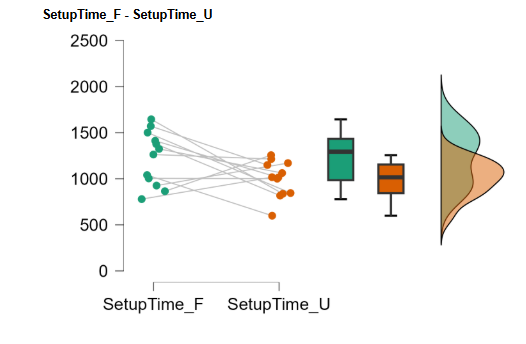
\includegraphics[width=0.62\linewidth]{media/media/image42.png}\end{center}

\phantomsection\addcontentsline{lof}{figure}{\protect\numberline{5.1}Setup time by condition.}%
\textbf{Figure 5.1} Setup time by condition. Raincloud plot showing the distribution, the box (median and interquartile range), and the individual participant values (N = 12) for the fragmented and unified conditions. Lower values indicate faster setup.
\end{figure}

Calibration time was shorter in the unified condition (M = 666.6 s, SD = 187.5) than in the fragmented condition (M = 925.9 s, SD = 262.2). As the normality assumption was met (Table 5.2), a paired-samples t-test was conducted. The difference was significant at the conventional α = .05 level, t(11) = 2.47, p = .031, dz = 0.71, 95\% CI {[}0.06, 1.34{]}, but did not meet the Bonferroni-adjusted threshold of α = .025 for the H1 family. The confidence interval excluding zero suggests a non-zero estimated effect, while the corrected hypothesis test remains non-significant. As shown in Figure 5.2, the reduction was fairly consistent in direction across participants.

\begin{figure}[H]
\begin{center}
\includegraphics[width=0.62\linewidth]{media/media/image11.png}\end{center}

\phantomsection\addcontentsline{lof}{figure}{\protect\numberline{5.2}Calibration time by condition.}%
\textbf{Figure 5.2} Calibration time by condition. Raincloud plot (N = 12) for the fragmented and unified conditions. Lower values indicate faster calibration.
\end{figure}

H1 predicted that participants would complete both setup and calibration significantly faster in the unified workflow. After correction, H1 is not supported: setup time did not differ significantly, and the calibration-time difference did not meet the adjusted threshold. The interpretation of the efficiency findings is developed in the Discussion (Chapter 6.2).

\hypertarget{perceived-workload-nasa-tlx-h2}{%
\subsubsection{5.1.2 Perceived workload, NASA-TLX (H2)}\label{perceived-workload-nasa-tlx-h2}}

Perceived workload was significantly lower in the unified condition (M = 22.22, SD = 18.83) than in the fragmented condition (M = 43.61, SD = 20.01), t(11) = 3.13, p = .010, dz = 0.90, 95\% CI {[}0.21, 1.57{]}. The effect was large and its confidence interval excluded zero. The distribution of scores by condition is shown in Figure 5.3. H2 is supported.

\begin{figure}[H]
\begin{center}
\includegraphics[width=0.62\linewidth]{media/media/image8.png}\end{center}

\phantomsection\addcontentsline{lof}{figure}{\protect\numberline{5.3}NASA-TLX workload by condition.}%
\textbf{Figure 5.3} NASA-TLX workload by condition. Raincloud plot (N = 12) for the fragmented and unified conditions. Higher values indicate greater perceived workload.
\end{figure}

\hypertarget{perceived-usability-sus-h3}{%
\subsubsection{5.1.3 Perceived usability, SUS (H3)}\label{perceived-usability-sus-h3}}

Perceived usability was significantly higher in the unified condition (M = 73.33, SD = 20.57) than in the fragmented condition (M = 46.46, SD = 30.22), t(11) = -3.21, p = .008, dz = -0.93, 95\% CI {[}-1.59, -0.23{]}. The effect was large and its confidence interval excluded zero. In absolute terms, the fragmented workflow scored below the commonly cited SUS benchmark of approximately 68 (Bangor et al., 2008) while the unified workflow scored above it. The distribution of scores by condition is shown in Figure 5.4. H3 is supported.

\begin{figure}[H]
\begin{center}
\includegraphics[width=0.62\linewidth]{media/media/image20.png}\end{center}

\phantomsection\addcontentsline{lof}{figure}{\protect\numberline{5.4}SUS scores by condition.}%
\textbf{Figure 5.4} SUS scores by condition. Raincloud plot (N = 12) for the fragmented and unified conditions. Higher values indicate greater perceived usability.
\end{figure}

\hypertarget{calibration-confidence-secondary-measure}{%
\subsubsection{5.1.4 Calibration confidence (secondary measure)}\label{calibration-confidence-secondary-measure}}

Calibration confidence is a secondary measure not tied to any of the five hypotheses. Calibration confidence was slightly higher in the unified condition (M = 5.75, SD = 1.42) than in the fragmented condition (M = 5.08, SD = 2.02). However, this difference was not statistically significant, t(11) = -0.82, p = .428, dz = -0.24, 95\% CI {[}-0.81, 0.34{]}. The estimated effect was small, and the confidence interval included zero, indicating substantial uncertainty about both the direction and magnitude of the effect. As illustrated in Figure 5.5, participant-level changes varied in both directions. Calibration confidence is therefore interpreted as broadly similar across the two conditions, while the individual differences are examined further in the qualitative findings in Chapter 5.2.1.

\begin{figure}[H]
\begin{center}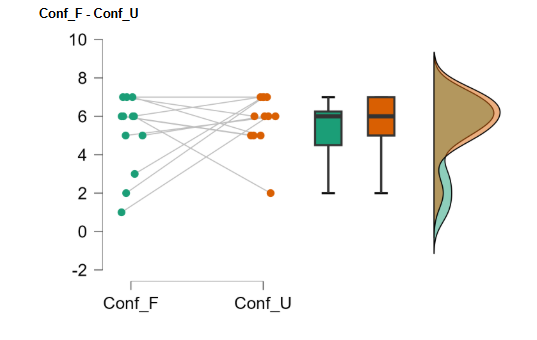
\includegraphics[width=0.62\linewidth]{media/media/image39.png}\end{center}

\phantomsection\addcontentsline{lof}{figure}{\protect\numberline{5.5}Self-rated calibration confidence by condition.}%
\textbf{Figure 5.5} Self-rated calibration confidence by condition. Raincloud plot (N = 12) for the fragmented and unified conditions, on the 1 to 7 rating scale. Higher values indicate greater confidence. The overlap between conditions reflects the two-directional pattern discussed in Chapter 5.2.1.
\end{figure}

\hypertarget{interaction-breakdowns-h4}{%
\subsubsection{5.1.5 Interaction breakdowns (H4)}\label{interaction-breakdowns-h4}}

Interaction breakdowns were significantly fewer in the unified condition (M = 8.17, SD = 4.06) than in the fragmented condition (M = 20.00, SD = 4.61), t(11) = 6.67, p \textless{} .001, dz = 1.93, 95\% CI {[}0.94, 2.89{]}. This was the largest effect in the study. As shown in Figure 5.6, the reduction was near-universal at the participant level, with almost every paired line sloping downward. H4 is supported

\begin{figure}[H]
\begin{center}
\includegraphics[width=0.62\linewidth]{media/media/image7.png}\end{center}

\phantomsection\addcontentsline{lof}{figure}{\protect\numberline{5.6}Interaction breakdowns by condition.}%
\textbf{Figure 5.6} Interaction breakdowns by condition. Raincloud plot (N = 12) for the fragmented and unified conditions. Higher values indicate more observed breakdowns.
\end{figure}

\Needspace{25\baselineskip}
To show where this reduction occurred, the total breakdown count was decomposed into the five recorded categories (Table 5.3). The reduction was concentrated almost entirely in two categories: hesitation periods fell from 129 occurrences in the fragmented condition to 34 in the unified condition, and requests for clarification fell from 76 to 30, together accounting for 141 of the 142-count total reduction. The remaining categories were small in both conditions: repeated calibration attempts (8 versus 6) and incorrect sequence execution (17 versus 12) fell modestly, while repeated baseline recording was the one category that rose in the unified condition (10 versus 16). This increase is examined in the Discussion (Chapter 6.6).

\begin{longtable}[]{@{}
  >{\raggedright\arraybackslash}p{(\columnwidth - 8\tabcolsep) * \real{0.4136}}
  >{\raggedright\arraybackslash}p{(\columnwidth - 8\tabcolsep) * \real{0.1708}}
  >{\raggedright\arraybackslash}p{(\columnwidth - 8\tabcolsep) * \real{0.1349}}
  >{\raggedright\arraybackslash}p{(\columnwidth - 8\tabcolsep) * \real{0.1439}}
  >{\raggedright\arraybackslash}p{(\columnwidth - 8\tabcolsep) * \real{0.1169}}@{}}
\toprule\noalign{}
\begin{minipage}[t]{\linewidth}\raggedright
\textbf{Category}
\end{minipage} & \begin{minipage}[t]{\linewidth}\raggedright
\textbf{Fragmented total}
\end{minipage} & \begin{minipage}[t]{\linewidth}\raggedright
\textbf{Fragmented M}
\end{minipage} & \begin{minipage}[t]{\linewidth}\raggedright
\textbf{Unified total}
\end{minipage} & \begin{minipage}[t]{\linewidth}\raggedright
\textbf{Unified}

\textbf{M}
\end{minipage} \\
\begin{minipage}[t]{\linewidth}\raggedright
Repeated calibration attempts (eye tracker)
\end{minipage} & \begin{minipage}[t]{\linewidth}\raggedright
8
\end{minipage} & \begin{minipage}[t]{\linewidth}\raggedright
0.67
\end{minipage} & \begin{minipage}[t]{\linewidth}\raggedright
6
\end{minipage} & \begin{minipage}[t]{\linewidth}\raggedright
0.50
\end{minipage} \\
\begin{minipage}[t]{\linewidth}\raggedright
Incorrect sequence execution
\end{minipage} & \begin{minipage}[t]{\linewidth}\raggedright
17
\end{minipage} & \begin{minipage}[t]{\linewidth}\raggedright
1.42
\end{minipage} & \begin{minipage}[t]{\linewidth}\raggedright
12
\end{minipage} & \begin{minipage}[t]{\linewidth}\raggedright
1.00
\end{minipage} \\
\begin{minipage}[t]{\linewidth}\raggedright
Repeated baseline recording (EDA)
\end{minipage} & \begin{minipage}[t]{\linewidth}\raggedright
10
\end{minipage} & \begin{minipage}[t]{\linewidth}\raggedright
0.83
\end{minipage} & \begin{minipage}[t]{\linewidth}\raggedright
16
\end{minipage} & \begin{minipage}[t]{\linewidth}\raggedright
1.33
\end{minipage} \\
\begin{minipage}[t]{\linewidth}\raggedright
Hesitation period (\textgreater{} 5 s inactivity)
\end{minipage} & \begin{minipage}[t]{\linewidth}\raggedright
129
\end{minipage} & \begin{minipage}[t]{\linewidth}\raggedright
10.75
\end{minipage} & \begin{minipage}[t]{\linewidth}\raggedright
34
\end{minipage} & \begin{minipage}[t]{\linewidth}\raggedright
2.83
\end{minipage} \\
\begin{minipage}[t]{\linewidth}\raggedright
Request for clarification
\end{minipage} & \begin{minipage}[t]{\linewidth}\raggedright
76
\end{minipage} & \begin{minipage}[t]{\linewidth}\raggedright
6.33
\end{minipage} & \begin{minipage}[t]{\linewidth}\raggedright
30
\end{minipage} & \begin{minipage}[t]{\linewidth}\raggedright
2.50
\end{minipage} \\
\begin{minipage}[t]{\linewidth}\raggedright
\textbf{Total}
\end{minipage} & \begin{minipage}[t]{\linewidth}\raggedright
\textbf{240}
\end{minipage} & \begin{minipage}[t]{\linewidth}\raggedright
\textbf{20.00}
\end{minipage} & \begin{minipage}[t]{\linewidth}\raggedright
\textbf{98}
\end{minipage} & \begin{minipage}[t]{\linewidth}\raggedright
\textbf{8.17}
\end{minipage} \\
\midrule\noalign{}
\endhead
\bottomrule\noalign{}
\endlastfoot
\end{longtable}

\phantomsection\addcontentsline{lot}{table}{\protect\numberline{5.3}Interaction breakdowns by category and condition.}%
\textbf{Table 5.3} Interaction breakdowns by category and condition. Counts cover N = 12 participants per condition. Totals are the summed count across all participants; M is the mean per participant. The category counts sum to the total breakdown count analysed under H4.

\hypertarget{calibration-quality-h5}{%
\subsubsection{5.1.6 Calibration quality (H5)}\label{calibration-quality-h5}}

H5 held that the unified workflow would achieve calibration quality comparable to the fragmented workflow across gaze accuracy, gaze precision, and valid data yield, with first-pass calibration success no lower than in the fragmented workflow. The four dimensions form a single hypothesis family, corrected together at a Bonferroni-adjusted threshold of .0125 (Chapter 4.6), and are reported in turn.

\textbf{Gaze accuracy:} The difference scores departed from normality (Table 5.2), so a Wilcoxon signed-rank test was conducted. Gaze accuracy did not differ significantly between the fragmented condition (M = 2.03 degrees, SD = 2.25) and the unified condition (M = 1.28 degrees, SD = 0.66), W = 51.5, p = .346, r = 0.32, 95\% CI {[}-0.30, 0.75{]}. The departure from normality was driven by a single elevated fragmented-condition value (P01, 9.07 degrees), visible in Figure 5.7; the rank-based test limits its influence, and the value is discussed as an instrument limitation in Chapter 6.8. The confidence interval was wide, remaining compatible with effects in either direction, and a non-significant result does not establish equivalence; the finding is therefore read as consistent with the expectation of similar accuracy under the shared calibration engine, not as demonstrated equivalence (Chapter 4.6.1.5).

\begin{figure}[H]
\begin{center}
\includegraphics[width=0.62\linewidth]{media/media/image24.png}\end{center}

\phantomsection\addcontentsline{lof}{figure}{\protect\numberline{5.7}Gaze accuracy by condition.}%
\textbf{Figure 5.7} Gaze accuracy by condition. Raincloud plot (N = 12) for the fragmented and unified conditions, in degrees of visual angle. Higher values indicate poorer accuracy. The elevated fragmented-condition point is the P01 outlier noted in the text.
\end{figure}

\textbf{Gaze precision:} The difference scores also departed from normality (Table 5.2), so a Wilcoxon signed-rank test was conducted. Gaze precision was poorer in the unified condition (M = 1.29 degrees, SD = 1.27; higher values indicate poorer precision) than in the fragmented condition (M = 0.65 degrees, SD = 0.33), W = 8.5, p = .019, r = -0.78, 95\% CI {[}-0.93, -0.39{]}. The difference was significant at the conventional α = .05 level but did not meet the Bonferroni-adjusted threshold of α = .0125 for the H5 family. As shown in Figure 5.8, the unified-condition distribution contains two values well above the rest (P05 and P11). Possible reasons for this difference are examined in the Discussion (Chapter 6.5).

\begin{figure}[H]
\begin{center}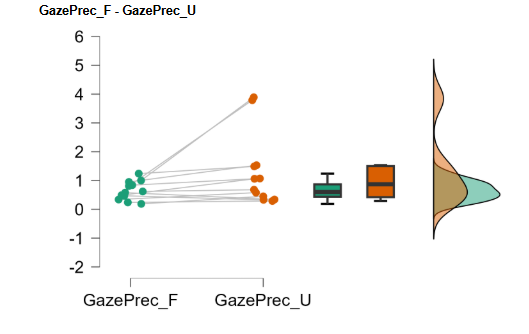
\includegraphics[width=0.62\linewidth]{media/media/image38.png}\end{center}

\phantomsection\addcontentsline{lof}{figure}{\protect\numberline{5.8}Gaze precision by condition.}%
\textbf{Figure 5.8} Gaze precision by condition. Raincloud plot (N = 12) for the fragmented and unified conditions, in degrees of visual angle. Higher values indicate poorer precision. The two elevated unified-condition points are P05 and P11, the two unified first-pass failures.
\end{figure}

\textbf{Valid data yield:} Valid data yield is the percentage of gaze samples collected during the five-point validation procedure that contained a valid binocular gaze estimate (Chapter 4.5.4). Yield was high in both conditions, meaning that almost all recorded gaze samples were usable (fragmented M = 99.54\%, SD = 1.13; unified M = 99.21\%, SD = 1.21). No significant difference was detected, t(11) = 0.70, p = .499, dz = 0.20, 95\% CI {[}-0.37, 0.77{]}. As shown in Figure 5.9, most values in both conditions lie between 98 and 100 percent, so the distributions are compressed against the upper bound of the scale.

\begin{figure}[H]
\begin{center}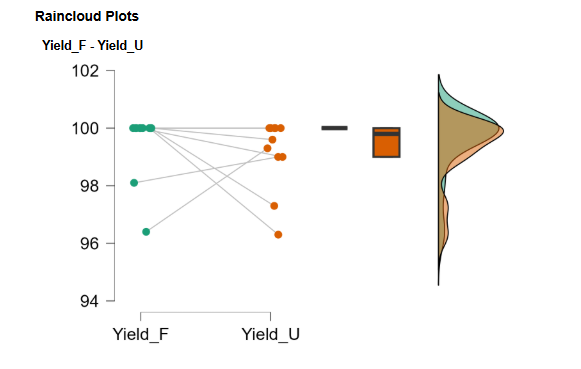
\includegraphics[width=0.62\linewidth]{media/media/image43.png}\end{center}

\phantomsection\addcontentsline{lof}{figure}{\protect\numberline{5.9}Valid data yield by condition.}%
\textbf{Figure 5.9} Valid data yield by condition. Raincloud plot (N = 12) showing the percentage of valid gaze samples for the fragmented and unified conditions. Higher values indicate greater yield.
\end{figure}

\textbf{First-pass calibration success:} First-pass calibration success records whether the calibration a participant committed to passed the validation on the first attempt (Chapter 4.5.4). Seven of twelve participants passed on the first attempt in the fragmented condition and nine of twelve in the unified condition; the full two-by-two contingency of paired outcomes is given in Table 5.4. Because the outcome is a paired binary variable, McNemar\textquotesingle s test was used (Chapter 4.6.1.3), in its exact binomial form given the six discordant pairs. The difference was not significant, p = .69. No significant difference in first-pass calibration success was found between the conditions.

\Needspace{13\baselineskip}
\begin{longtable}[]{@{}
  >{\raggedright\arraybackslash}p{(\columnwidth - 6\tabcolsep) * \real{0.3026}}
  >{\raggedright\arraybackslash}p{(\columnwidth - 6\tabcolsep) * \real{0.2594}}
  >{\raggedright\arraybackslash}p{(\columnwidth - 6\tabcolsep) * \real{0.2450}}
  >{\raggedright\arraybackslash}p{(\columnwidth - 6\tabcolsep) * \real{0.1729}}@{}}
\toprule\noalign{}
\begin{minipage}[t]{\linewidth}\raggedright
\end{minipage} & \begin{minipage}[t]{\linewidth}\raggedright
\textbf{Unified: Failed}
\end{minipage} & \begin{minipage}[t]{\linewidth}\raggedright
\textbf{Unified:Passed}
\end{minipage} & \begin{minipage}[t]{\linewidth}\raggedright
\textbf{Row Total}
\end{minipage} \\
\begin{minipage}[t]{\linewidth}\raggedright
\textbf{Fragmented: Failed}
\end{minipage} & \begin{minipage}[t]{\linewidth}\raggedright
1
\end{minipage} & \begin{minipage}[t]{\linewidth}\raggedright
4
\end{minipage} & \begin{minipage}[t]{\linewidth}\raggedright
5
\end{minipage} \\
\begin{minipage}[t]{\linewidth}\raggedright
\textbf{Fragmented: Passed}
\end{minipage} & \begin{minipage}[t]{\linewidth}\raggedright
2
\end{minipage} & \begin{minipage}[t]{\linewidth}\raggedright
5
\end{minipage} & \begin{minipage}[t]{\linewidth}\raggedright
7
\end{minipage} \\
\begin{minipage}[t]{\linewidth}\raggedright
\textbf{Column Total}
\end{minipage} & \begin{minipage}[t]{\linewidth}\raggedright
3
\end{minipage} & \begin{minipage}[t]{\linewidth}\raggedright
9
\end{minipage} & \begin{minipage}[t]{\linewidth}\raggedright
12
\end{minipage} \\
\midrule\noalign{}
\endhead
\bottomrule\noalign{}
\endlastfoot
\end{longtable}

\phantomsection\addcontentsline{lot}{table}{\protect\numberline{5.4}First-pass calibration success.}%
\textbf{Table 5.4} First-pass calibration success. Two-by-two contingency of first-attempt outcomes in the fragmented and unified conditions, with the exact McNemar test (N = 12; six discordant pairs).

After Bonferroni correction across the four-test family, none of the four dimensions reached the adjusted threshold of α = .0125. No significant differences were detected in gaze accuracy, valid data yield, or first-pass calibration success, and first-pass success was descriptively no lower in the unified condition, as H5 predicted. Gaze precision was the exception: the unified condition was poorer, with a difference that was significant before correction but not after it. H5 is therefore supported with one qualification concerning gaze precision, whose possible causes are examined in the Discussion (Chapter 6.5).

\hypertarget{eda-baseline-comparability-check}{%
\subsubsection{5.1.7 EDA baseline comparability check}\label{eda-baseline-comparability-check}}

The mean resting EDA baseline was recorded to check that participants\textquotesingle{} resting physiological starting levels, and the signal acquisition and microsiemens conversion producing them, were consistent across the two workflows (Chapter 4.5.5). It is not a scored calibration-quality outcome and is reported descriptively, with the accompanying paired test read only as a consistency check (Chapter 4.6.1.6). The two conditions showed similar baseline values (fragmented M = 4.53 uS, SD = 3.20; unified M = 5.56 uS, SD = 4.28), and the paired test was not significant, t(11) = -1.88, p = .087, dz = -0.54, 95\% CI {[}-1.14, 0.08{]}; the confidence interval did not provide clear evidence of a difference between the two conditions. The distribution of baseline values by condition is shown in Figure 5.10.

\begin{center}
\includegraphics[width=0.62\linewidth]{media/media/image15.png}\end{center}
\phantomsection\addcontentsline{lof}{figure}{\protect\numberline{5.10}Mean resting EDA baseline by condition.}%
\textbf{Figure 5.10} Mean resting EDA baseline by condition. Raincloud plot (N = 12) in microsiemens for the fragmented and unified conditions.

\Needspace{21\baselineskip}
\hypertarget{summary-of-quantitative-results}{%
\subsubsection{5.1.8 Summary of quantitative results}\label{summary-of-quantitative-results}}

The table reports each measure with its descriptive statistics, the reported test, the exact p-value, the effect size and its 95 percent confidence interval, the family threshold, and the outcome after correction.

\begingroup\let\small\footnotesize\setlength{\tabcolsep}{4pt}
\begin{longtable}[]{@{}
  >{\raggedright\arraybackslash}p{(\columnwidth - 12\tabcolsep) * \real{0.1713}}
  >{\raggedright\arraybackslash}p{(\columnwidth - 12\tabcolsep) * \real{0.1491}}
  >{\raggedright\arraybackslash}p{(\columnwidth - 12\tabcolsep) * \real{0.1263}}
  >{\raggedright\arraybackslash}p{(\columnwidth - 12\tabcolsep) * \real{0.1339}}
  >{\raggedright\arraybackslash}p{(\columnwidth - 12\tabcolsep) * \real{0.0602}}
  >{\raggedright\arraybackslash}p{(\columnwidth - 12\tabcolsep) * \real{0.2062}}
  >{\raggedright\arraybackslash}p{(\columnwidth - 12\tabcolsep) * \real{0.1330}}@{}}
\toprule\noalign{}
\begin{minipage}[t]{\linewidth}\raggedright
\textbf{Measure}
\end{minipage} & \begin{minipage}[t]{\linewidth}\raggedright
\textbf{Fragmented M (SD)}
\end{minipage} & \begin{minipage}[t]{\linewidth}\raggedright
\textbf{Unified M (SD)}
\end{minipage} & \begin{minipage}[t]{\linewidth}\raggedright
\textbf{Test}
\end{minipage} & \begin{minipage}[t]{\linewidth}\raggedright
\textbf{p}
\end{minipage} & \begin{minipage}[t]{\linewidth}\raggedright
\textbf{Effect Size (95\% CI)}
\end{minipage} & \begin{minipage}[t]{\linewidth}\raggedright
\textbf{Threshold}
\end{minipage} \\
\begin{minipage}[t]{\linewidth}\raggedright
Setup time (s)
\end{minipage} & \begin{minipage}[t]{\linewidth}\raggedright
1226 (292.7)
\end{minipage} & \begin{minipage}[t]{\linewidth}\raggedright
998.4 (193.4)
\end{minipage} & \begin{minipage}[t]{\linewidth}\raggedright
t(11) = 2.03
\end{minipage} & \begin{minipage}[t]{\linewidth}\raggedright
0.067
\end{minipage} & \begin{minipage}[t]{\linewidth}\raggedright
dz = 0.59 {[}-0.04, 1.19{]}
\end{minipage} & \begin{minipage}[t]{\linewidth}\raggedright
.025 (H1)
\end{minipage} \\
\begin{minipage}[t]{\linewidth}\raggedright
Calibration time (s)
\end{minipage} & \begin{minipage}[t]{\linewidth}\raggedright
925.9 (262.2)
\end{minipage} & \begin{minipage}[t]{\linewidth}\raggedright
666.6 (187.5)
\end{minipage} & \begin{minipage}[t]{\linewidth}\raggedright
t(11) = 2.47
\end{minipage} & \begin{minipage}[t]{\linewidth}\raggedright
.031
\end{minipage} & \begin{minipage}[t]{\linewidth}\raggedright
dz = 0.71 {[}0.06, 1.34{]}
\end{minipage} & \begin{minipage}[t]{\linewidth}\raggedright
.025 (H1)
\end{minipage} \\
\begin{minipage}[t]{\linewidth}\raggedright
NASA-TLX
\end{minipage} & \begin{minipage}[t]{\linewidth}\raggedright
43.61 (20.01)
\end{minipage} & \begin{minipage}[t]{\linewidth}\raggedright
22.22 (18.83)
\end{minipage} & \begin{minipage}[t]{\linewidth}\raggedright
t(11) = 3.13
\end{minipage} & \begin{minipage}[t]{\linewidth}\raggedright
.010
\end{minipage} & \begin{minipage}[t]{\linewidth}\raggedright
dz = 0.90 {[}0.21, 1.57{]}
\end{minipage} & \begin{minipage}[t]{\linewidth}\raggedright
.05 (H2)
\end{minipage} \\
\begin{minipage}[t]{\linewidth}\raggedright
SUS
\end{minipage} & \begin{minipage}[t]{\linewidth}\raggedright
46.46 (30.22)
\end{minipage} & \begin{minipage}[t]{\linewidth}\raggedright
73.33 (20.57)
\end{minipage} & \begin{minipage}[t]{\linewidth}\raggedright
t(11) = -3.21
\end{minipage} & \begin{minipage}[t]{\linewidth}\raggedright
.008
\end{minipage} & \begin{minipage}[t]{\linewidth}\raggedright
dz = -0.93 {[}-1.59, -0.23{]}
\end{minipage} & \begin{minipage}[t]{\linewidth}\raggedright
.05 (H3)
\end{minipage} \\
\begin{minipage}[t]{\linewidth}\raggedright
Breakdowns
\end{minipage} & \begin{minipage}[t]{\linewidth}\raggedright
20.00 (4.61)
\end{minipage} & \begin{minipage}[t]{\linewidth}\raggedright
8.17 (4.06)
\end{minipage} & \begin{minipage}[t]{\linewidth}\raggedright
t(11) = 6.67
\end{minipage} & \begin{minipage}[t]{\linewidth}\raggedright
\textless{} .001
\end{minipage} & \begin{minipage}[t]{\linewidth}\raggedright
dz = 1.93 {[}0.94, 2.89{]}
\end{minipage} & \begin{minipage}[t]{\linewidth}\raggedright
.05 (H4)
\end{minipage} \\
\begin{minipage}[t]{\linewidth}\raggedright
Gaze accuracy (deg)
\end{minipage} & \begin{minipage}[t]{\linewidth}\raggedright
2.03 (2.25)
\end{minipage} & \begin{minipage}[t]{\linewidth}\raggedright
1.28 (0.66)
\end{minipage} & \begin{minipage}[t]{\linewidth}\raggedright
Wilcoxon = 51.5
\end{minipage} & \begin{minipage}[t]{\linewidth}\raggedright
.346
\end{minipage} & \begin{minipage}[t]{\linewidth}\raggedright
r = 0.32 {[}-0.30, 0.75{]}
\end{minipage} & \begin{minipage}[t]{\linewidth}\raggedright
.0125 (H5)
\end{minipage} \\
\begin{minipage}[t]{\linewidth}\raggedright
Gaze precision (deg)
\end{minipage} & \begin{minipage}[t]{\linewidth}\raggedright
0.65 (0.33)
\end{minipage} & \begin{minipage}[t]{\linewidth}\raggedright
1.29 (1.27)
\end{minipage} & \begin{minipage}[t]{\linewidth}\raggedright
Wilcoxon = 8.5
\end{minipage} & \begin{minipage}[t]{\linewidth}\raggedright
.019
\end{minipage} & \begin{minipage}[t]{\linewidth}\raggedright
r = -0.78 {[}-0.93, -0.39{]}
\end{minipage} & \begin{minipage}[t]{\linewidth}\raggedright
.0125 (H5)
\end{minipage} \\
\begin{minipage}[t]{\linewidth}\raggedright
Valid data yield (\%)
\end{minipage} & \begin{minipage}[t]{\linewidth}\raggedright
99.54 (1.13)
\end{minipage} & \begin{minipage}[t]{\linewidth}\raggedright
99.21 (1.21)
\end{minipage} & \begin{minipage}[t]{\linewidth}\raggedright
t(11) = 0.70
\end{minipage} & \begin{minipage}[t]{\linewidth}\raggedright
.499
\end{minipage} & \begin{minipage}[t]{\linewidth}\raggedright
dz = 0.20 {[}-0.37, 0.77{]}
\end{minipage} & \begin{minipage}[t]{\linewidth}\raggedright
.0125 (H5)
\end{minipage} \\
\begin{minipage}[t]{\linewidth}\raggedright
Confidence (1-7)
\end{minipage} & \begin{minipage}[t]{\linewidth}\raggedright
5.08 (2.02)
\end{minipage} & \begin{minipage}[t]{\linewidth}\raggedright
5.75 (1.42)
\end{minipage} & \begin{minipage}[t]{\linewidth}\raggedright
t(11) = -0.82
\end{minipage} & \begin{minipage}[t]{\linewidth}\raggedright
.428
\end{minipage} & \begin{minipage}[t]{\linewidth}\raggedright
dz = -0.24 {[}-0.81, 0.34{]}
\end{minipage} & \begin{minipage}[t]{\linewidth}\raggedright
secondary
\end{minipage} \\
\begin{minipage}[t]{\linewidth}\raggedright
EDA baseline (uS)
\end{minipage} & \begin{minipage}[t]{\linewidth}\raggedright
4.53 (3.20)
\end{minipage} & \begin{minipage}[t]{\linewidth}\raggedright
5.56 (4.28)
\end{minipage} & \begin{minipage}[t]{\linewidth}\raggedright
t(11) = -1.88
\end{minipage} & \begin{minipage}[t]{\linewidth}\raggedright
.087
\end{minipage} & \begin{minipage}[t]{\linewidth}\raggedright
dz = -0.54 {[}-1.14, 0.08{]}
\end{minipage} & \begin{minipage}[t]{\linewidth}\raggedright
comparability
\end{minipage} \\
\midrule\noalign{}
\endhead
\bottomrule\noalign{}
\endlastfoot
\end{longtable}
\endgroup

\phantomsection\addcontentsline{lot}{table}{\protect\numberline{5.5}Paired comparisons between conditions.}%
\textbf{Table 5.5} Paired comparisons between conditions. Reported are exact p-values, effect sizes with 95 percent confidence intervals, family-wise thresholds, and the outcomes after per-hypothesis Bonferroni correction (N = 12).

After per-hypothesis Bonferroni correction, the picture by hypothesis is as follows. For H1, neither timing measure reached the corrected threshold: setup time did not differ significantly, and calibration time favoured the unified workflow with a medium-to-large effect and an interval excluding zero but did not meet the Bonferroni-adjusted threshold of α = .025. H2, H3, and H4 were each supported: workload fell, usability rose, and breakdowns fell sharply, the last the largest effect in the study, all with confidence intervals excluding zero. For H5, no dimension reached the corrected threshold. No significant differences were detected in gaze accuracy, valid data yield, or first-pass calibration success, with first-pass success descriptively no lower in the unified condition. Gaze precision was the exception: the unified condition was poorer, with a difference that was significant before correction but not after it. H5 is therefore supported with one qualification concerning gaze precision. Calibration confidence and the EDA baseline, which are not tied to any hypothesis, showed small differences with intervals spanning zero.

\hypertarget{qualitative-findings}{%
\subsection{5.2 Qualitative Findings}\label{qualitative-findings}}

The written open-ended post-task responses, the open-ended questionnaire item, and the researcher observation notes were analysed using reflexive thematic analysis, following the procedure described in Chapter 4.6.2. These findings complement the quantitative results by explaining the patterns behind them: they identify where and why participants struggled in each workflow (RQ1) and how the two workflows shaped workload, usability, and confidence in the calibration (RQ3). Codes were tagged by condition so that the themes speak directly to the comparison between workflows.

Five themes were developed. The first four describe participants\textquotesingle{} direct experience of the two workflows: confidence grounded in system feedback (Theme 1, speaking primarily to RQ3), the burden of coordinating fragmented tools (Theme 2, speaking primarily to RQ1), and the guidance the unified workflow provided and the gaps it left (Themes 3 and 4, speaking to both RQ1 and RQ3). The fifth theme is a methodological caution rather than an experiential finding, concerning familiarity and order effects across the two sessions. Participant extracts are presented verbatim and unedited, and are attributed by participant and condition.

\hypertarget{theme-1-confidence-grounded-in-system-feedback}{%
\subsubsection{\texorpdfstring{5.2.1 Theme 1: Confidence grounded in system feedback }{5.2.1 Theme 1: Confidence grounded in system feedback }}\label{theme-1-confidence-grounded-in-system-feedback}}

Participants' confidence in the calibration depended mainly on system feedback rather than actual success. Clear confirmation reassured them, while a lack of feedback created uncertainty and often led them to assume that the calibration had failed.

In the fragmented workflow the absence of any confirmation was felt directly. One participant completed the setup but could not judge it, writing that they "didn't get a validation that I am correctly doing it" (P01, Fragmented), and assigned a confidence rating of 3. Another described being sure only that data was being captured, not that it was good: they were "confident something was being read... but wasn\textquotesingle t confident of the quality of the data, only that something was being recorded" (P09, Fragmented). The same participants responded to the unified workflow\textquotesingle s visible confirmations in almost the opposite terms. P01, who had assigned a rating of 3 in the fragmented condition, rose to 7 and explained it simply: "The green ticks and the progress bar assured me that I am on right track" (P01, Unified). P04 attributed their confidence directly to the confirmation message, "CALIBRATION DONE SUCCESSFULLY" (P04, Unified), and P09 valued the system surfacing information they could not otherwise access: "I love that it\textquotesingle s giving me metrics as a non professional" (P09, Unified).

Visible feedback did not always increase confidence. When the system indicated unusual readings, some participants became concerned: P03 tried to regulate their breathing while viewing the live EDA graph, and P06 reported that an unexpectedly high reading reduced their confidence. Thus, feedback made confidence more responsive to the apparent quality of the data rather than simply increasing it. This may also explain the absence of an overall difference in confidence between conditions: increases for most participants were partly offset by decreases among those who noticed problematic readings .

\hypertarget{theme-2-the-burden-of-coordinating-fragmented-tools}{%
\subsubsection{\texorpdfstring{5.2.2 Theme 2: The burden of coordinating fragmented tools }{5.2.2 Theme 2: The burden of coordinating fragmented tools }}\label{theme-2-the-burden-of-coordinating-fragmented-tools}}

The main difficulty in the fragmented workflow was not any single tool, but the need to coordinate several disconnected systems. Each used a different interface and terminology, requiring participants to track progress across tools and manage the transitions between them. This coordination effort emerged as a substantial source of burden.

The most concrete expression was the sheer number of moving parts. One participant recounted having "to open multiple tabs... two different softwares for the devices... and download data from both which can sometimes feel a little too much" (P02, Fragmented). The Jupyter and Python step used to compute the EDA value was a distinct and severe barrier for participants without a coding background: one found "The python codes are very tiny and not understandable by every user" (P01, Fragmented), and another, on reaching it, "had absolutely no idea what to do" (P04, Fragmented). The recording software contributed its own recurring failure, with several participants pressing play instead of record, and the cumulative effect was summarized by the participant who "felt overwhelmed, lost and frustrated" because "each software has a different workflow and UI" (P10, Fragmented). The near-absence of this theme from the unified data is itself part of the finding: when the tools were consolidated, the work of stitching them together disappeared from participants\textquotesingle{} accounts.

\hypertarget{theme-3-guidance-from-the-system}{%
\subsubsection{5.2.3 Theme 3: Guidance from the system}\label{theme-3-guidance-from-the-system}}

The unified workflow was experienced as accessible specifically because it led participants through the process one step at a time and made expert decisions on their behalf, rather than assuming knowledge they did not have. This was expressed most strongly by the less experienced participants.

Participants repeatedly attributed the ease to being guided. One described being "guided step by step through the calibration process... very easy because there were instructions that I just had to follow" (P04, Unified). Another contrasted the one-at-a-time structure with being shown everything at once: it "took me through the journey with one step at a time instead of overwhelming me {[}with{]} all data and instruction at one go" (P12, Unified). The sensor recommendation was received as help rather than constraint, captured in one participant\textquotesingle s real-time realization, "I didn\textquotesingle t choose these sensors! - oh it\textquotesingle s recommending them to me, I get it" (P03, Unified). The fragmented counterpart to this theme is the felt absence of such guidance, where "the steps were definitely missing large gaps of information on how to get to each point" (P09, Fragmented), which links this theme back to the overhead described in Theme 2 (see Chapter 5.2.2).

\hypertarget{theme-4-the-limits-of-guidance}{%
\subsubsection{5.2.4 Theme 4: The limits of guidance}\label{theme-4-the-limits-of-guidance}}

Although the unified workflow provided more guidance, uncertainty remained when instructions were unclear, values were not explained, or feedback suggested a possible problem. This theme therefore highlights the limitations of the guided workflow.

Two residual gaps stand out. The first is interpretation: participants were shown an EDA value but not told what it meant. One wrote that "The value is given in μS, but I don\textquotesingle t know what to make of it" (P04, Unified), and another, shown a low reading highlighted in red, "doubted that I sticked the sensors wrong... there\textquotesingle s no way to check it" (P10, Unified). The second is electrode placement, which several participants got wrong despite the on-screen instruction, with one noting that "the picture in the setup should have been more precise" (P06, Unified). This placement issue warrants a specific clarification, because it is easy to misread as a fault of the unified interface alone. The placement illustration was inherited from the OpenSignals manufacturer manual and appeared in both conditions, on the Sensa screen in the unified workflow and on the paper reference sheet in the fragmented one. The confusion it caused is therefore a shared instructional-artefact problem that both workflows carried from the same source, rather than a unified-specific design failure. Its limitations simply became most visible where the image appeared on screen during the guided flow. Alongside these, a recurring preference for less text and more visual guidance ran across both conditions, expressed plainly as "I\textquotesingle d like to have more images and less text" (P10, Unified).

\hypertarget{theme-5-familiarity-and-order-effects}{%
\subsubsection{\texorpdfstring{5.2.5 Theme 5: Familiarity and order effects }{5.2.5 Theme 5: Familiarity and order effects }}\label{theme-5-familiarity-and-order-effects}}

The final theme is interpretive rather than experiential and concerns familiarity and order effects. Part of the ease participants reported reflected prior exposure rather than the workflow itself: one participant stated that the unified task felt easier "because I had already gone through a similar process with the fragmented task, I had some idea of what to expect" (P07, Unified). Ease of this kind results from having completed the other condition first and cannot be attributed to the workflow design. The counterbalanced design distributes this effect across the two condition orders rather than eliminating it, and it is treated as a limitation in Chapter 6.8.

\hypertarget{summary-of-qualitative-findings}{%
\subsubsection{5.2.6 Summary of qualitative findings}\label{summary-of-qualitative-findings}}

Across the five themes, participants\textquotesingle{} accounts converge on a coherent contrast. The fragmented workflow left the system state hidden and made participants carry the overhead of several disconnected tools, which undermined their ability to judge their own success. The unified workflow addressed both issues by making state visible and by leading participants through the process, which most experienced as easier and more reassuring. The account is not one-sided: visible feedback also surfaced problems and lowered some participants\textquotesingle{} confidence, guidance did not resolve every ambiguity, and a shared instructional artefact caused placement errors in both conditions. The integration of these themes with the quantitative results, and their implications for design, are taken up in Chapter 6.


\clearpage
\hypertarget{discussion}{%
\section{6. Discussion}\label{discussion}}

\hypertarget{overview}{%
\subsection{6.1 Overview}\label{overview}}

This chapter interprets the quantitative results and qualitative themes together to assess whether a unified, guided workflow improves setup efficiency, perceived workload, usability, and interaction stability relative to a fragmented multi-tool baseline, while preserving eye-tracking calibration quality (Chapter 1.3). The evidence provides a consistent, though not entirely uniform, answer and highlights broader implications for the design of onboarding and calibration workflows in multi-sensor research platforms.

Overall, the unified workflow produced substantial improvements in perceived workload, usability, and interaction stability compared with the fragmented baseline. Perceived workload was lower and perceived usability was higher in the unified condition, both with large effects whose intervals excluded zero (H2, H3), and interaction breakdowns fell sharply, the largest effect in the study (H4). Efficiency moved in the same direction: setup and calibration times were both faster in the unified condition, and the calibration-time advantage was of medium-to-large size, though neither timing measure reached the family-wise-corrected threshold (H1). Calibration quality, treated throughout as a validity safeguard rather than a target, showed no significant differences in gaze accuracy, valid data yield, or first-pass success, and was poorer in the unified condition on one dimension, gaze precision (H5).

The qualitative themes explain much of this pattern: they locate the fragmented workflow\textquotesingle s cost in the effort of coordinating disconnected tools, attribute the unified workflow\textquotesingle s ease to step-by-step guidance, and show that making system state visible could raise or lower participants\textquotesingle{} confidence depending on what it revealed.

Two features of the study frame how these results should be read, both set out in Chapter 4.6. First, with twelve participants the paired comparisons can reliably detect only large effects, so a non-significant result is not evidence that the workflows do not differ; effect sizes and their confidence intervals are therefore given interpretive weight alongside the significance decisions. Second, the same Tobii Core engine performed the eye-tracking calibration in both conditions, so any difference in calibration outcomes or in calibration time reflects the surrounding workflow rather than the calibration algorithm itself. The remainder of the chapter takes each hypothesis in turn, integrating the relevant qualitative themes, then considers the role of visible feedback (Chapter 6.6) before turning to design implications (Chapter 6.7) and limitations (Chapter 6.8).

\hypertarget{setup-and-calibration-efficiency-h1}{%
\subsection{6.2 Setup and calibration efficiency (H1)}\label{setup-and-calibration-efficiency-h1}}

H1 predicted that participants would complete both setup and calibration significantly faster in the unified workflow. Both measures favoured the unified condition, and the calibration-time effect was of medium-to-large size. However, neither measure remained significant after the Bonferroni correction, so H1 was not supported. The study therefore cannot confirm that the unified workflow is faster, although both measures pointed that way.

Owing to the same Tobii calibration procedure being run in both conditions, any time difference reflects the surrounding workflow rather than the calibration algorithm itself. The qualitative findings suggest why: the fragmented workflow required additional tool-switching, navigation, and clarification, whereas the unified workflow organized these steps into a guided sequence. This would also explain why the reduction was clearer for calibration time than for the broader setup-time measure, since calibration is where the fragmented workflow\textquotesingle s tool-switching is densest. Reduced procedural overhead of this kind corresponds to the preparation burden described in prior work on multi-sensor setups (Aloi et al., 2024; Zhu \& Lv, 2023).

\hypertarget{perceived-workload-and-usability-h2-h3}{%
\subsection{6.3 Perceived workload and usability (H2, H3)}\label{perceived-workload-and-usability-h2-h3}}

Participants reported significantly lower workload and higher usability in the unified condition, supporting H2 and H3. In absolute terms, the SUS score moved from below the commonly cited benchmark of approximately 68 (Bangor et al., 2008) in the fragmented condition to above it in the unified condition. Together, these findings indicate that integrating the individual steps into a guided workflow made the process less demanding and easier to use.

The qualitative findings provide a clear explanation for this improvement. In the fragmented condition, participants had to coordinate several tools and workflows, which frequently caused confusion and frustration. In contrast, the unified workflow provided step-by-step guidance and reduced the number of decisions participants had to make independently. The results therefore suggest that guidance and workflow integration are particularly beneficial for inexperienced users, who cannot rely on prior knowledge when difficulties occur.

Although demand characteristics may have influenced the subjective ratings, the corresponding reduction in observed interaction breakdowns supports the conclusion that the benefits were not limited to participants\textquotesingle{} perceptions.

\hypertarget{interaction-breakdowns-h4-1}{%
\subsection{6.4 Interaction breakdowns (H4)}\label{interaction-breakdowns-h4-1}}

The unified workflow reduced observable interaction breakdowns, and the reduction was concentrated in hesitation periods and requests for clarification (Table 5.3). This was the largest and most consistent effect in the study, holding for nearly every participant, and H4 is supported. Since breakdowns are an observed behavioural count rather than a self-report, this result is the least vulnerable to the demand-characteristics concern raised for the subjective measures, and it is the study\textquotesingle s strongest single piece of evidence that the two workflows differ in behaviour and not only in how they were rated.

The concentration of the reduction in hesitation and clarification-seeking answers RQ1 directly: what makes fragmented setups slow and effortful is predominantly uncertainty, not procedural error. Both categories mark moments in which a participant did not know whether a step had succeeded or what to do next. Where the fragmented workflow left "large gaps of information on how to get to each point" (P09, Fragmented), the unified workflow closed those gaps with step sequencing and explicit confirmation. The hard-error categories were small in both conditions, so the unified workflow\textquotesingle s benefit was not that it prevented procedural mistakes but that it removed the uncertainty surrounding each step. This mechanism also connects the breakdown result to the preceding chapters: time spent paused in uncertainty adds to setup and calibration time (Chapter 6.2), and the effort of not knowing how to proceed is a component of perceived workload (Chapter 6.3).

One secondary finding ran against the overall pattern: repeated baseline recordings rose in the unified condition. The increase is small and local and does not disturb the overall result; it is examined in Chapter 6.6 as part of the two-directional role of visible feedback.

\hypertarget{calibration-quality-h5-1}{%
\subsection{6.5 Calibration quality (H5)}\label{calibration-quality-h5-1}}

For calibration quality, no clear differences were found in gaze accuracy, valid data yield, or first-pass calibration success, while gaze precision was poorer in the unified condition. H5, framed as a comparability claim because the same Tobii Core engine performs the calibration in both conditions and Sensa\textquotesingle s validation layer only scores the result (Chapters 1.5 and 4.6), is therefore supported with one qualification.

On gaze accuracy, valid data yield, and first-pass success, no significant differences were detected, which is consistent with the expectation that the shared calibration engine would produce similar outcomes in both conditions. Since no equivalence testing was conducted, these results cannot demonstrate that the workflows are equivalent (Chapter 4.6.1.5); they show only that the study found no evidence of degradation. Within that limit, the safeguard held: the usability improvements reported in the preceding chapters were not accompanied by any detectable loss on these three dimensions.

The gaze-precision difference requires more care. Two sessions, P05 and P11, accounted for the elevated unified mean, and these were also the two sessions with the lowest valid-data yields in that condition (below 97.5 percent, against 99 percent or above for everyone else).

A tentative explanation is that tracking was less stable in these two sessions. Momentary tracking failures produce invalid samples, which lower the valid-data yield, and a low proportion of valid samples is itself an indication that the system is having difficulty tracking a particular individual or environment (Holmqvist et al., 2012, p. 48). The same unstable conditions increase the scatter of the samples that are successfully recorded, which worsens precision, since precision is a measure of sample dispersion and the standard-deviation estimator used here is specifically sensitive to environmental instability (Holmqvist et al., 2012, p. 48).

A comparable pattern appears in the fragmented condition, where the guided workflow was absent and the two lowest-yield participants also recorded among the poorest precision values, which suggests the association reflects a general property of tracking stability rather than an effect of the unified design. The explanation nonetheless remains tentative: the study cannot establish why tracking was less stable for these two participants in the unified condition specifically, and poorer precision cannot be conclusively attributed to data quality rather than to the workflow.

The study therefore provides no evidence that the usability improvements degraded gaze accuracy, valid data yield, or first-pass calibration success. It does show poorer gaze precision in the unified condition, concentrated in two sessions, and the present data cannot resolve the cause. Whether the unified workflow systematically affects precision would need a larger study with per-session tracking logs.

The interface fault observed during calibration is addressed among the design implications (Chapter 6.7), and the measurement limitations of the custom validation instrument among the limitations (Chapter 6.8).

\hypertarget{the-two-directional-role-of-visible-system-state}{%
\subsection{\texorpdfstring{6.6 The two-directional role of visible system state }{6.6 The two-directional role of visible system state }}\label{the-two-directional-role-of-visible-system-state}}

A mechanism running through several of the results is that visible system state could either increase or decrease participants\textquotesingle{} confidence. In the fragmented workflow, which reported little about its own state, participants were left to infer success and often inferred wrongly. In the unified workflow, visible confirmations raised confidence for most participants, while for a few the same visibility lowered it because a displayed reading suggested a problem (Chapter 5.2.1). This two-directional movement offers an explanation for the absence of an overall difference in calibration confidence between the conditions (Chapter 5.1.4): increases for most participants were partly offset by decreases among those who noticed problematic readings.

The same mechanism accounts for the one breakdown category that rose in the unified condition: repeated baseline recordings increased because the live feedback gave participants a concrete reason to re-record; a possibility that the fragmented workflow never surfaced. A possible interpretation is that visible feedback made confidence responsive to the apparent quality of the data rather than uniformly increasing it, which for a research tool would be a desirable property, since an operator\textquotesingle s confidence should track the state of the setup rather than be uniformly high. This interpretation is consistent with the qualitative pattern but cannot be confirmed by the present data, because the relationship between confidence and actual setup quality was not directly analysed.

\hypertarget{design-implications}{%
\subsection{6.7 Design implications}\label{design-implications}}

Three residual usability problems remained in the unified workflow (Theme 4). First, some values were displayed without interpretation: participants welcomed seeing metrics, but a baseline value in microsiemens meant nothing to them, and an unexplained low reading flagged in red produced doubt rather than insight. Second, several participants placed the electrodes incorrectly despite the on-screen instruction. The placement illustration was inherited from the OpenSignals manufacturer manual and appeared in both conditions, on screen in the unified workflow and on the paper reference sheet in the fragmented one, so the confusion is a shared instructional-artefact problem rather than a fault of the unified interface; its limitations simply became most visible during the guided flow. Third, participants in both conditions expressed a preference for less on-screen text and more visual guidance. In addition, one first-pass calibration failure was traced to a design oversight: the validation control was not gated behind a completed calibration, and two similarly weighted primary actions appeared on the same screen, allowing a participant to attempt validation before calibrating (Figure 3.14).

These findings translate into four direct recommendations for multi-sensor onboarding workflows. First, apply error-prevention gating consistently: the validation step for eye-tracking should be disabled until a calibration has been completed, and no screen should present two similarly weighted primary actions. Second, pair every displayed metric with interpretation, such as a plain-language reference range or a short statement of what a good value looks like, so that visibility informs rather than alarms. Third, replace the inherited manufacturer placement illustration with a purpose-made, step-by-step sequence showing each action separately, such as applying the gel electrodes and then connecting the sensor cable to its port, whether as sequential illustrations or a short animation. Fourth, reduce on-screen text in favour of diagrams and short demonstrations at the steps where participants stalled.

Underlying these recommendations is the principle the study supports: a guided workflow\textquotesingle s advantage comes from making system state visible and leading the operator through it. Visibility must be paired with interpretation, and the workflow\textquotesingle s own safeguards must be applied to every step without exception, including the steps that check the workflow\textquotesingle s own output.

\hypertarget{limitations}{%
\subsection{6.8 Limitations}\label{limitations}}

The limitations of the study fall into four groups: sample size, measurement, scope, and generalisability.

\textbf{Sample size:} With twelve participants, the paired comparisons can reliably detect only large effects (approximately dz = 0.9 at 80 percent power), and the per-family Bonferroni correction reduces power further. Non-significant results therefore cannot be read as evidence of no difference. This restricts the conclusions on H1 and on gaze precision in particular: the corrected verdicts say only that the study could not confirm those differences, not that they are absent. The study is best read as detecting the large differences it was designed to detect and as silent on smaller ones.

\textbf{Measurement:} The eye tracker was a consumer-grade Tobii 4C, so the calibration-quality findings should not be assumed to transfer to research-grade systems. Meanwhile, the custom validation layer has not been benchmarked against a reference-grade instrument, so its absolute accuracy and precision values are instrument-relative and cannot be read as externally calibrated. The fixed per-target collection window produced one artefactual accuracy value (P01), which the rank-based analysis contained but did not remove. The calibration-confidence measure was a single Likert item and is therefore a weak operationalisation of its construct.

\textbf{Scope:} Only eye tracking and EDA were connected and measured; EEG and ECG appeared as selectable options but were never recorded. The findings therefore apply to a two-modality subset of the platform\textquotesingle s intended scope, and a workflow spanning four sensors, with more electrodes and longer preparation, might behave differently. The EDA baseline was reported only as a descriptive comparability check, so the study cannot comment on biosensor calibration quality. The live signal-quality indicators shown during EDA setup use thresholds that were set empirically during development rather than derived from a published physiological standard

\textbf{Generalisability}: The sample was a convenience sample of students and staff at a single university, tested by a single experimenter in one laboratory, which limits transfer to professional UX and HCI researchers, to other sites and tasks, and to field conditions. Demand characteristics cannot be excluded for the self-report measures, since a participant who inferred that the unified workflow was the author\textquotesingle s own system might have rated it more favourably. Order and familiarity effects carry over between conditions despite counterbalancing (Theme 5), so part of the reported ease may reflect prior exposure rather than the workflow. For the qualitative strand, the coder was also the designer of the workflow and while this dual role was addressed through reflexive analysis and the full coding documentation in Appendix L, single-coder interpretation remains a limitation. Finally, the cause of the poorer gaze precision in the unified condition cannot be conclusively established: its association with low valid-data yield in two sessions suggests unstable tracking, but an effect of the workflow itself cannot be ruled out.

Within these limits, the study supports a bounded conclusion: in this laboratory context, with this hardware and task, the unified workflow substantially improved perceived workload, usability, and interaction stability without detectable degradation of gaze accuracy, valid data yield, or first-pass calibration success, while the gaze-precision difference remains unresolved.

\clearpage
\hypertarget{conclusion-and-future-work}{%
\section{7. Conclusion and Future Work}\label{conclusion-and-future-work}}

\hypertarget{summary-and-conclusions}{%
\subsection{7.1 Summary and conclusions}\label{summary-and-conclusions}}

This thesis set out to build and empirically evaluate an integrated, usability-centred onboarding and calibration workflow for multi-sensor research environments, and to compare it against a fragmented workflow built from separate per-modality tools. The two sensors contributed different setup demands: eye tracking involved calibration-quality indicators, EDA involved baseline establishment and sensor readiness. The calibration-quality indicators were carried as a validity safeguard, to check that usability gains did not come at the cost of data quality.

The study used a within-subjects, counterbalanced design with twelve participants, each completing both workflows. It combined objective performance measures, validated subjective instruments, eye-tracking calibration indicators, EDA setup and baseline measures, and a reflexive thematic analysis of participants\textquotesingle{} written accounts.

\textbf{For RQ1,} which examined the steps and breakdowns that contributed most to completion time, the findings point primarily to uncertainty rather than error. Hesitations and requests for clarification (both indicating that participants were unsure whether a step had been completed successfully or what they should do next) accounted for nearly the entire difference between the two workflows. By contrast, explicit procedural errors were rare in both conditions. The main cost of the fragmented workflow, therefore, was not incorrect action but the uncertainty created when participants were left to determine the system state and the next step for themselves.

\textbf{For RQ2,} the unified workflow reduced calibration time significantly, with a medium-to-large effect. Setup time was also shorter in the unified condition, although this difference was not statistically significant. The findings therefore provide clear evidence of improved calibration efficiency, but only tentative evidence of faster setup. Both measures favoured the unified workflow, but after correction for multiple comparisons neither difference remained statistically significant. The study therefore cannot confirm that the unified workflow is faster, although both measures pointed that way, and the reduction was clearer for calibration time than for setup time. A likely interpretation, though not something the study establishes, is that this reflects the calibration phase being where the fragmented workflow\textquotesingle s tool-switching is densest.

\textbf{For RQ3,} the effect on workload, usability, and confidence, the results differ across the three measures. Perceived workload was roughly halved and perceived usability rose from below to above the established benchmark, both large effects on validated instruments. Calibration confidence, by contrast, did not change on average. The qualitative data explains this flat average: making the system state visible could raise confidence by confirming progress, but it could also lower confidence by revealing a problem that would have gone unnoticed in the fragmented workflow, and these two movements offset each other across participants.

\textbf{For RQ4,} the effect on calibration quality, the two workflows showed no significant differences in gaze accuracy, valid data yield, or first-pass calibration success, which is what would be expected given that the same calibration engine operates in both conditions. Gaze precision was the exception: it was poorer in the unified condition, and this was driven by two participants who also recorded the lowest valid-data yields in that condition. Since low yield means fewer usable samples, and unstable tracking would tend to reduce both the number of samples and their consistency, the probable reading is that these two sessions had less stable tracking and that the workflow itself did not worsen precision. The same association between low yield and poorer precision also appeared in the fragmented condition, where the guided workflow was absent. H5 is therefore supported for gaze accuracy, valid data yield, and first-pass success, and qualified for gaze precision, whose cause the study cannot resolve.

Taken together, restructuring the onboarding and calibration of a multi-sensor setup as a single guided flow produced large improvements in perceived workload, perceived usability, and interaction stability. It also reduced calibration time, though not by a margin the study can confirm. It did this without any detected loss of gaze accuracy, valid data yield, or first-pass calibration success.

The themes and the breakdown analysis suggest why. The unified workflow makes the system state visible and leads the operator through it, which removes much of the uncertainty that makes fragmented setups slow and effortful.

However, visibility cuts both ways, and this has a design consequence worth stating. A visible system state can lower an operator\textquotesingle s confidence when it surfaces a real problem. In a research tool that is arguably what should happen: confidence should follow the actual state of the setup rather than stay uniformly high. The study did not test whether confidence tracked setup quality, so this is a design consideration rather than a result.

\hypertarget{contributions}{%
\subsection{7.2 Contributions}\label{contributions}}

This thesis makes four contributions, all concerning the onboarding and calibration workflow that the author designed and evaluated. They do not extend to the other Sensa components the workflow relies on: the EDA conversion, the HDF5 storage pipeline, the recording and visualization modules, and the platform infrastructure were built by other contributors and integrated into the workflow rather than developed as part of this work.

\textbf{The first contribution is a design artefact:} a unified, usability-centred onboarding and calibration workflow that integrates the full setup sequence, from study and sensor selection through calibration, validation, and biosensor baseline recording, into a single guided flow. Its contribution is to take usability principles that are normally left to disconnected per-tool interfaces, guided selection, step-by-step placement, readiness checks, and corrective feedback, and realize them as one coherent sequence for multi-sensor setup. The author designed the full workflow, its information architecture, interaction flow, and interface, and implemented several of its components, including the eye-tracking validation layer, the live positioning metrics, and the derived EDA signal-quality indicators; the design and implementation are set out in Chapter 3.

\textbf{The second contribution is methodological:} an eye-tracking validation layer that produces an interpretable, quantitative measure of calibration quality in-flow. Instead of relying on the calibration engine\textquotesingle s qualitative gaze-trace, it presents a five-point validation grid and computes angular gaze accuracy and precision, scored against a pass threshold and returned to the operator immediately. The author designed and implemented this layer; its methodological basis is set out in Chapter 3.3.4. Its absolute values are instrument-relative, since it has not been benchmarked against a reference-grade system. Within the study, it provided the consistent calibration measure that made the H5 validity check possible.

\textbf{The third contribution is empirical:} a controlled, within-subjects comparison of the unified workflow against a realistic fragmented baseline, measuring efficiency, workload, usability, interaction stability, and calibration quality together. Measuring usability and data quality in the same study, rather than separately, is what lets the study show that the usability gains did not cost eye-tracking data quality. This depends on treating calibration quality as a validity safeguard rather than a performance target, measured with the same validation layer in both conditions.

\textbf{The fourth contribution is analytic:} a five-category taxonomy of interaction breakdowns, showing that hesitations and requests for clarification, rather than procedural errors, were the main sources of additional time and effort in the fragmented workflow. This answers RQ1 and grounds the design implications in Chapter 6.7.

\hypertarget{future-work}{%
\subsection{7.3 Future work}\label{future-work}}

Several methodological steps follow from the study\textquotesingle s limitations (Chapter 6.8). The most important is an adequately powered replication: the present sample reliably detects only large differences, so the medium-sized setup-time advantage, the finer structure of the subjective measures, and the yield-precision relationship, which here rests on only two low-yield sessions, all warrant a larger sample. The eye-tracking validation layer should also be benchmarked against a reference-grade system, which would let its current instrument-relative accuracy and precision values be read as ground-truth rather than within-study comparisons. The evaluation should also move beyond a single site, a single experimenter, and a convenience sample of students and staff towards other researchers, other laboratories, and eventually field conditions. A design that separates genuine workflow ease from the order and familiarity effects noted in Theme 5 would further sharpen the causal reading.

A second set of steps concerns the workflow itself, set out in Chapter 6.7. The most important is to close the interface-gating gap behind the study\textquotesingle s one documented first-pass artefact: the validation control should be disabled until calibration is complete, and the calibration screen should not offer two similarly weighted primary actions. The recommendation step should also be made conditional on the selected study goal and available hardware rather than showing a fixed recommendation, with a check that the researcher\textquotesingle s final selections are appropriate for the stated goal. Beyond that, surfaced values should be paired with plain-language reference ranges so that visibility informs rather than alarms, the shared electrode-placement illustration should be replaced with a purpose-made step-by-step diagram, and the steps where participants stalled should use diagrams and short demonstrations rather than dense text. Making the validation dwell time configurable, or re-showing any target that fails to collect enough valid samples, would prevent the validation layer from reporting a value it lacks the data to compute.

Finally, the workflow should be evaluated across the full set of sensors the platform targets. Only eye tracking and EDA were connected and measured in this study. Extending it to EEG and ECG, which require additional electrodes and longer preparation, would show whether the reductions in workload and interaction breakdowns scale with setup complexity or diminish as more sensors are added. Once the platform\textquotesingle s remaining components are complete, the whole Sensa approach could be evaluated end to end, with all four sensors, in the research settings the platform is intended for.


\clearpage
\hypertarget{list-of-references}{%
\section{\texorpdfstring{List of References }{List of References }}\label{list-of-references}}

\begingroup
\setlength{\parindent}{-0.5in}\setlength{\leftskip}{0.5in}\setlength{\parskip}{6pt plus 2pt minus 1pt}

\hspace*{-0.5in}Aloi, D., Bouzit, S., \& Li, J. (2024). Biometric methods for user research: Three case studies. \emph{Extended Abstracts of the CHI Conference on Human Factors in Computing Systems}, 1--8. \url{https://doi.org/10.1145/3613905.3637132}

Amani, S., Obeidat, N., Ferris, T., \& Shryock, K. (2024). \emph{Enhancing the onboarding experience with wearable technology for research applications}. 2024 AHFE International Conference on Human Factors in Design, Engineering, and Computing. \url{https://doi.org/10.54941/ahfe1005662}

Bangor, A., Kortum, P. T., \& Miller, J. T. (2008). An empirical evaluation of the System Usability Scale. \emph{International Journal of Human--Computer Interaction, 24}(6), 574--594. \url{https://doi.org/10.1080/10447310802205776}

Braun, V., \& Clarke, V. (2006). Using thematic analysis in psychology. \emph{Qualitative Research in Psychology, 3}(2), 77--101. \url{https://doi.org/10.1191/1478088706qp063oa}

Braun, V., \& Clarke, V. (2019). Reflecting on reflexive thematic analysis. \emph{Qualitative Research in Sport, Exercise and Health, 11}(4), 589--597. \url{https://doi.org/10.1080/2159676X.2019.1628806}

Brooke, J. (1996). SUS: A quick and dirty usability scale. In P. W. Jordan, B. Thomas, B. A. Weerdmeester, \& I. L. McClelland (Eds.), \emph{Usability evaluation in industry} (pp. 189--194). Taylor \& Francis.

Consensus NLP Inc. (2026). \emph{Consensus: AI-powered academic search} {[}Computer software{]}. \url{https://consensus.app}

Corporation for Digital Scholarship. (2026). \emph{Zotero} (Version 7.x) {[}Computer software{]}. \url{https://www.zotero.org}

Cuve, H. C., Stojanov, J., Roberts-Gaal, X., Catmur, C., \& Bird, G. (2022). Validation of Gazepoint low-cost eye-tracking and psychophysiology bundle. \emph{Behavior Research Methods, 54}(2), 1027--1049. \url{https://doi.org/10.3758/s13428-021-01654-x}

Dalrymple, K. A., Manner, M. D., Harmelink, K. A., Teska, E. P., \& Elison, J. T. (2018). An examination of recording accuracy and precision from eye tracking data from toddlerhood to adulthood. \emph{Frontiers in Psychology, 9}, 803. \url{https://doi.org/10.3389/fpsyg.2018.00803}

Dell Inc. (2016). \emph{Tobii Eye Tracker user\textquotesingle s guide} (Alienware 17 R4, Rev. A00). Dell Inc.

Drewes, H., Pfeuffer, K., \& Alt, F. (2019). Time- and space-efficient eye tracker calibration. \emph{Proceedings of the 11th ACM Symposium on Eye Tracking Research \& Applications}, 1--8. \url{https://doi.org/10.1145/3314111.3319818}

Figma Inc. (2026). \emph{Figma} {[}Computer software{]}. \url{https://www.figma.com}

Gaspar-Figueiredo, D., Vanderdonckt, J., Abrahão, S., \& Insfran, E. (2026). User experience with adaptive user interfaces: Comparing performance and preferences. \emph{Journal of Systems and Software, 231}, 112598. \url{https://doi.org/10.1016/j.jss.2025.112598}

Guo, F., Li, M., Hu, M., Li, F., \& Lin, B. (2019). Distinguishing and quantifying the visual aesthetics of a product: An integrated approach of eye-tracking and EEG. \emph{International Journal of Industrial Ergonomics, 71}, 47--56. \url{https://doi.org/10.1016/j.ergon.2019.02.006}

Hart, S. G. (2006). NASA-Task Load Index (NASA-TLX); 20 years later. \emph{Proceedings of the Human Factors and Ergonomics Society Annual Meeting, 50}(9), 904--908. \url{https://doi.org/10.1177/154193120605000909}

Hart, S. G., \& Staveland, L. E. (1988). Development of NASA-TLX (Task Load Index): Results of empirical and theoretical research. In P. A. Hancock \& N. Meshkati (Eds.), \emph{Human mental workload} (Vol. 52, pp. 139--183). North-Holland. \url{https://doi.org/10.1016/S0166-4115(08)62386-9}

Holmqvist, K., Nyström, M., \& Mulvey, F. (2012). Eye tracker data quality: What it is and how to measure it. \emph{Proceedings of the Symposium on Eye Tracking Research and Applications}, 45--52. \url{https://doi.org/10.1145/2168556.2168563}

iMotions A/S. (2026). \emph{iMotions Lab} (Version 11) {[}Computer software{]}. iMotions A/S. \url{https://imotions.com/products/imotions-lab/}

JASP Team. (2026). \emph{JASP} (Version 0.98.0) {[}Computer software{]}. \url{https://jasp-stats.org}

Mikalef, P., Sharma, K., Chatterjee, S., Chaudhuri, R., Parida, V., \& Gupta, S. (2023). All eyes on me: Predicting consumer intentions on social commerce platforms using eye-tracking data and ensemble learning. \emph{Decision Support Systems, 175}, 114039. \url{https://doi.org/10.1016/j.dss.2023.114039}

Nielsen, J. (1994). \emph{10 usability heuristics for user interface design}. Nielsen Norman Group. \url{https://www.nngroup.com/articles/ten-usability-heuristics/}

Notion Labs Inc. (2026). \emph{Notion} {[}Computer software{]}. \url{https://www.notion.so}

Nyström, M., Andersson, R., Holmqvist, K., \& Van De Weijer, J. (2013). The influence of calibration method and eye physiology on eyetracking data quality. \emph{Behavior Research Methods, 45}(1), 272--288. \url{https://doi.org/10.3758/s13428-012-0247-4}

OBS Project Contributors. (2026). OBS Studio (Version 32.1.2) {[}Computer software{]}. \url{https://obsproject.com}

PLUX Wireless Biosignals, S.A. (2020). \emph{Electrodermal activity (EDA) sensor datasheet} (Rev. B). PLUX Wireless Biosignals, S.A. \url{https://support.pluxbiosignals.com/wp-content/uploads/2021/11/Electrodermal_Activity_EDA_Datasheet.pdf}

PLUX Wireless Biosignals, S.A. (2026). \emph{OpenSignals (r)evolution} (Public build 2026-04-08) {[}Computer software{]}. PLUX Wireless Biosignals, S.A. \url{https://www.pluxbiosignals.com/pages/opensignals}

Rhine-Waal University of Applied Sciences. (2026). \emph{Katalog PLUS} {[}Library discovery portal{]}. \url{https://hsrw.eu/library}

Tobii AB. (2021). \emph{Tobii Eye Tracking Core Software} (Version 2.16.8.214) {[}Computer software{]}. Tobii AB. \url{https://gaming.tobii.com/getstarted/?bundle=tobii-core-4c}

Tobii AB. (2025). \emph{Tobii Pro Lab} (Version 25.7) {[}Computer software{]}. Tobii AB. \url{https://www.tobii.com/products/software/behavior-research-software/tobii-pro-lab}

Van Lier, H. G., Pieterse, M. E., Garde, A., Postel, M. G., De Haan, H. A., Vollenbroek-Hutten, M. M. R., Schraagen, J. M., \& Noordzij, M. L. (2020). A standardized validity assessment protocol for physiological signals from wearable technology: Methodological underpinnings and an application to the E4 biosensor. \emph{Behavior Research Methods, 52}(2), 607--629. \url{https://doi.org/10.3758/s13428-019-01263-9}

Zhu, L., \& Lv, J. (2023). Review of studies on user research based on EEG and eye tracking. \emph{Applied Sciences, 13}(11), 6502. \url{https://doi.org/10.3390/app13116502}


\endgroup

\clearpage
\hypertarget{appendices}{%
\section{\texorpdfstring{Appendices }{Appendices }}\label{appendices}}

\clearpage
\hypertarget{appendix-l}{%
\subsection{Appendix A: Screenshots of Fragmented workflow tools}\label{appendix-l}}

This appendix presents screenshots of the three tools used in the fragmented condition, shown as participants encountered them: the Tobii Core eye-tracking software (Figures A.1 to A.6), the OpenSignals biosignal software (Figures A.7 to A.10), and the JupyterLab script used to compute the mean EDA value (Figures A.11 and A.12). They are included to make the fragmented workflow concrete alongside the interface figures shown for the unified workflow in Chapter 3.

\begin{figure}[H]
\begin{center}
\includegraphics[height=0.36\textheight,max width=\linewidth,keepaspectratio]{media/media/image17.png}\end{center}

\phantomsection\addcontentsline{lof}{figure}{\protect\numberline{A.1}Tobii Core sidetray.}%
\textbf{Figure A.1} Tobii Core sidetray. The user is shown options to toggle on/off the eye tracker, or navigate to Games and Experience, Interactions, Display Setup, Gaze Trace, and option to set up a new profile by clicking on the left arrow at the bottom.
\end{figure}

\vspace{1.5em}


\begin{figure}[H]
\begin{center}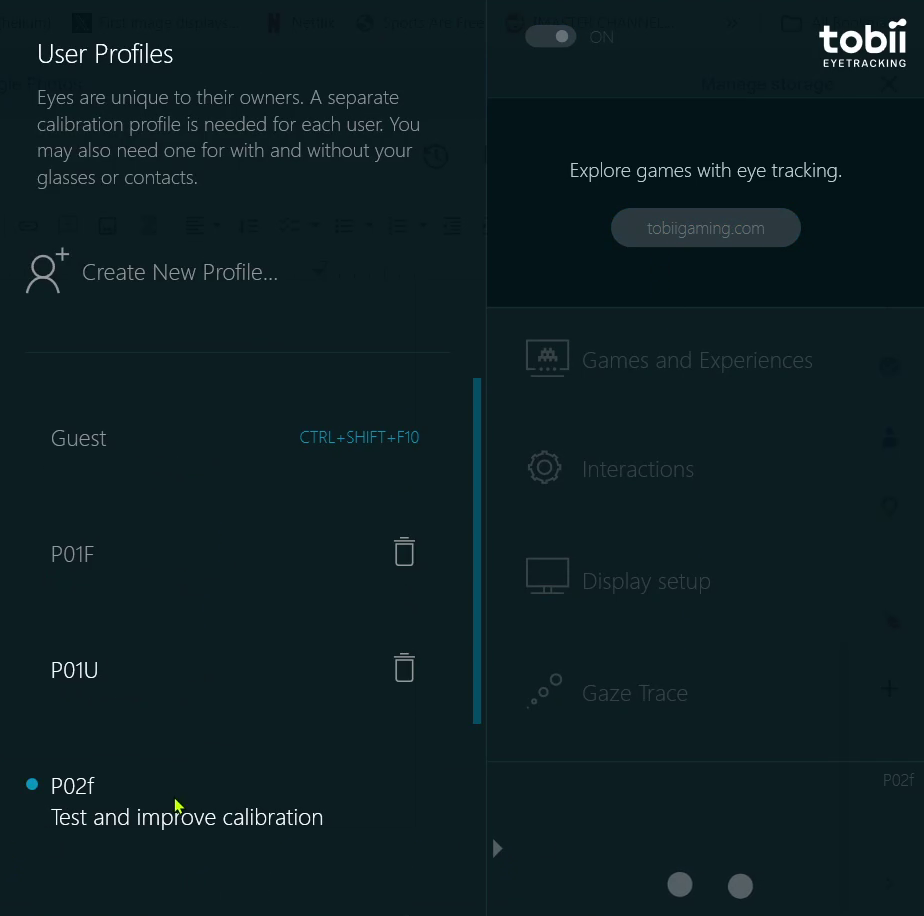
\includegraphics[height=0.34\textheight,max width=\linewidth,keepaspectratio]{media/media/image40.png}\end{center}

\phantomsection\addcontentsline{lof}{figure}{\protect\numberline{A.2}Tobii Core expanded sidetray.}%
\textbf{Figure A.2} Tobii Core expanded sidetray. The user is shown the option to Create a New Profile or use an existing one.
\end{figure}

\vspace{1.5em}


\begin{figure}[H]
\begin{center}
\includegraphics[height=0.34\textheight,max width=\linewidth,keepaspectratio]{media/media/image26.png}\end{center}

\phantomsection\addcontentsline{lof}{figure}{\protect\numberline{A.3}Tobii Core calibration sequence Step 1.}%
\textbf{Figure A.3} Tobii Core calibration sequence Step 1. Live eye detection is shown and communicated to the user.
\end{figure}

\vspace{1.5em}


\begin{figure}[H]
\begin{center}
\includegraphics[height=0.34\textheight,max width=\linewidth,keepaspectratio]{media/media/image23.png}\end{center}

\phantomsection\addcontentsline{lof}{figure}{\protect\numberline{A.4}Tobii Core calibration sequence Step 2.}%
\textbf{Figure A.4} Tobii Core calibration sequence Step 2. The user is shown instructions ``Look at each dot until it explodes'' about what to do in the next step.
\end{figure}

\vspace{1.5em}


\begin{figure}[H]
\begin{center}
\includegraphics[height=0.34\textheight,max width=\linewidth,keepaspectratio]{media/media/image10.png}\end{center}

\phantomsection\addcontentsline{lof}{figure}{\protect\numberline{A.5}Tobii Core calibration sequence Step 3.}%
\textbf{Figure A.5} Tobii Core calibration sequence Step 3. The user is shown 3 dots, which explode when the user focuses on them. This sequence is conducted twice.
\end{figure}

\vspace{1.5em}


\begin{figure}[H]
\begin{center}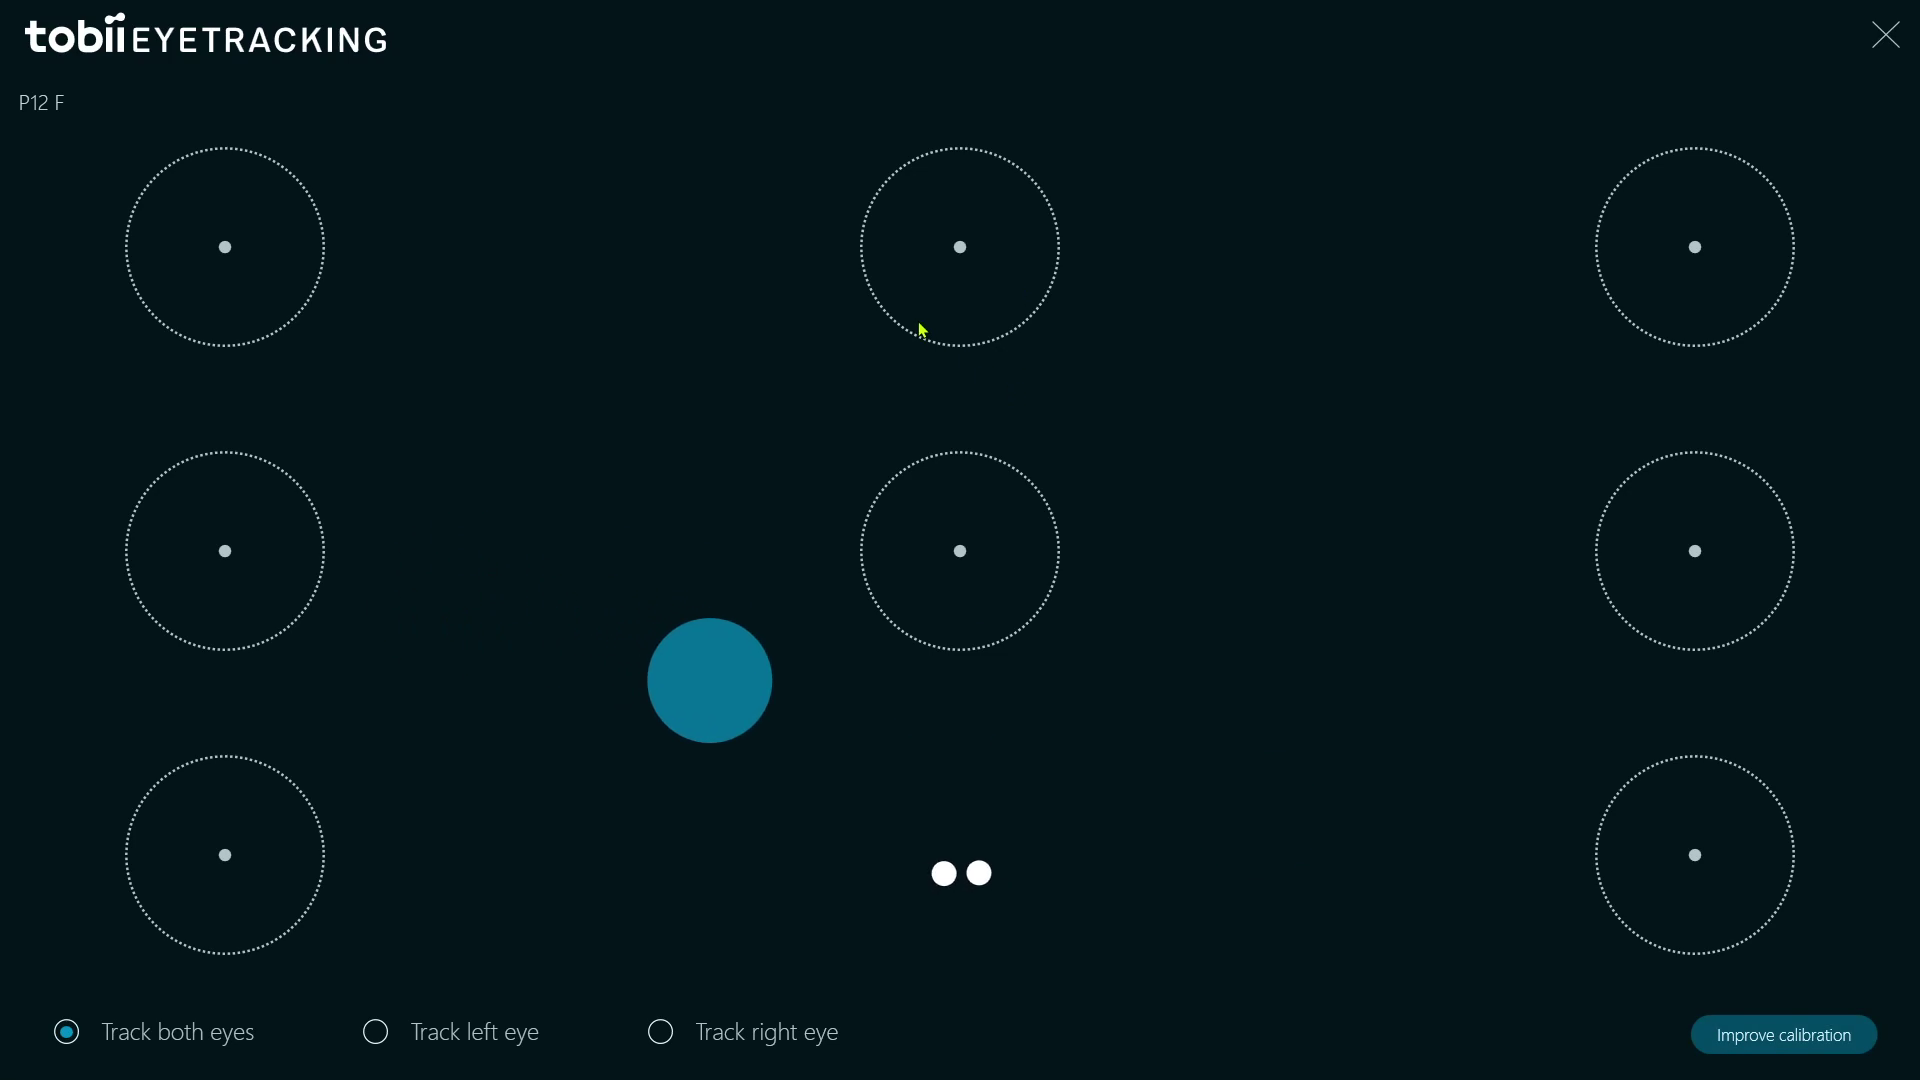
\includegraphics[height=0.34\textheight,max width=\linewidth,keepaspectratio]{media/media/image41.png}\end{center}

\phantomsection\addcontentsline{lof}{figure}{\protect\numberline{A.6}Tobii Core validation.}%
\textbf{Figure A.6} Tobii Core validation. Test and Improve calibration opens a qualitative eye tracking validation screen. The user is presented with a 9 point grid and can trace their gaze across the screen with a blue pointer, and choose to track either their left, right, or both eyes.
\end{figure}

\vspace{1.5em}


\begin{figure}[H]
\begin{center}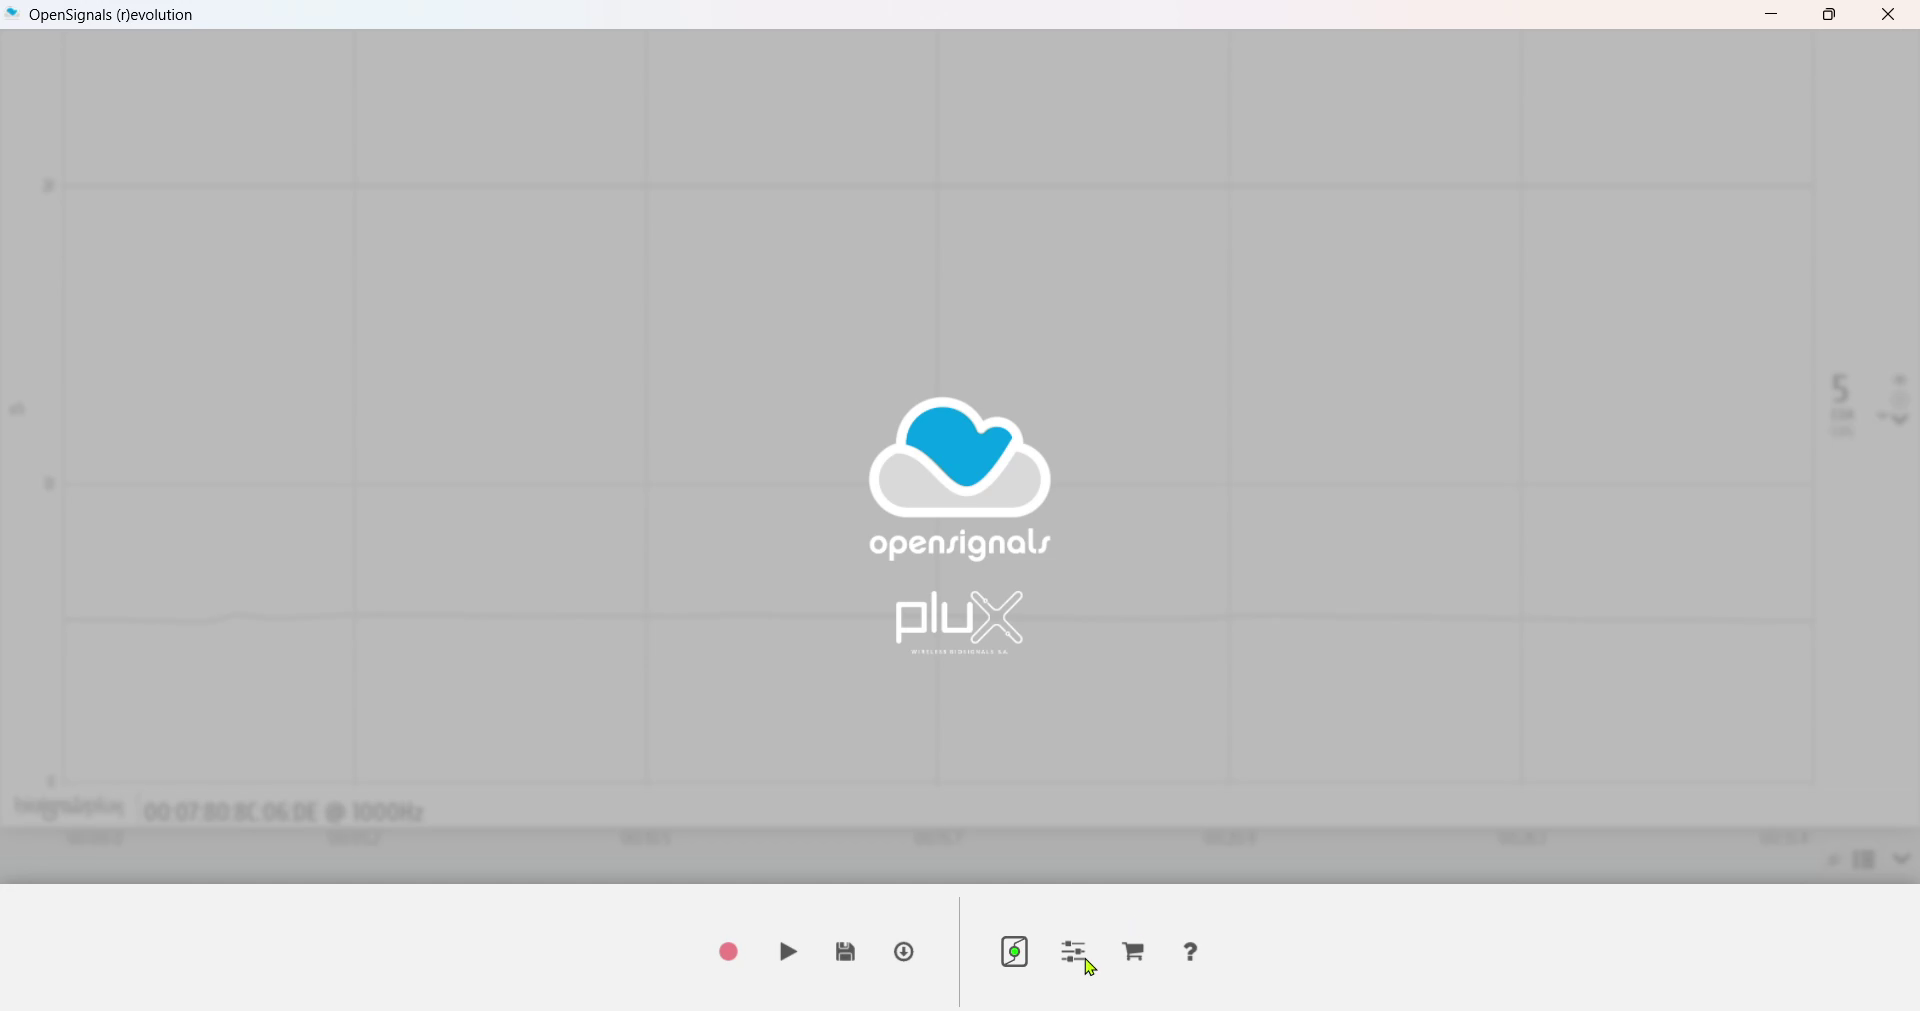
\includegraphics[height=0.34\textheight,max width=\linewidth,keepaspectratio]{media/media/image32.png}\end{center}

\phantomsection\addcontentsline{lof}{figure}{\protect\numberline{A.7}OpenSignals Main Screen.}%
\textbf{Figure A.7} OpenSignals Main Screen . The user is shown an interface with buttons for record, play, save, export, hub status (green for enabled, red for disabled), settings, cart and help.
\end{figure}

\vspace{1.5em}


\begin{figure}[H]
\begin{center}
\includegraphics[height=0.34\textheight,max width=\linewidth,keepaspectratio]{media/media/image13.png}\end{center}

\phantomsection\addcontentsline{lof}{figure}{\protect\numberline{A.8}OpenSignals Live Hub Status Screen.}%
\textbf{Figure A.8} OpenSignals Live Hub Status Screen . The user is shown the list of known and new items found, along with a status card depicting the MAC and Physical address of the connected hardware. The user can choose to enable or disable the connection as well.
\end{figure}

\vspace{1.5em}


\begin{figure}[H]
\begin{center}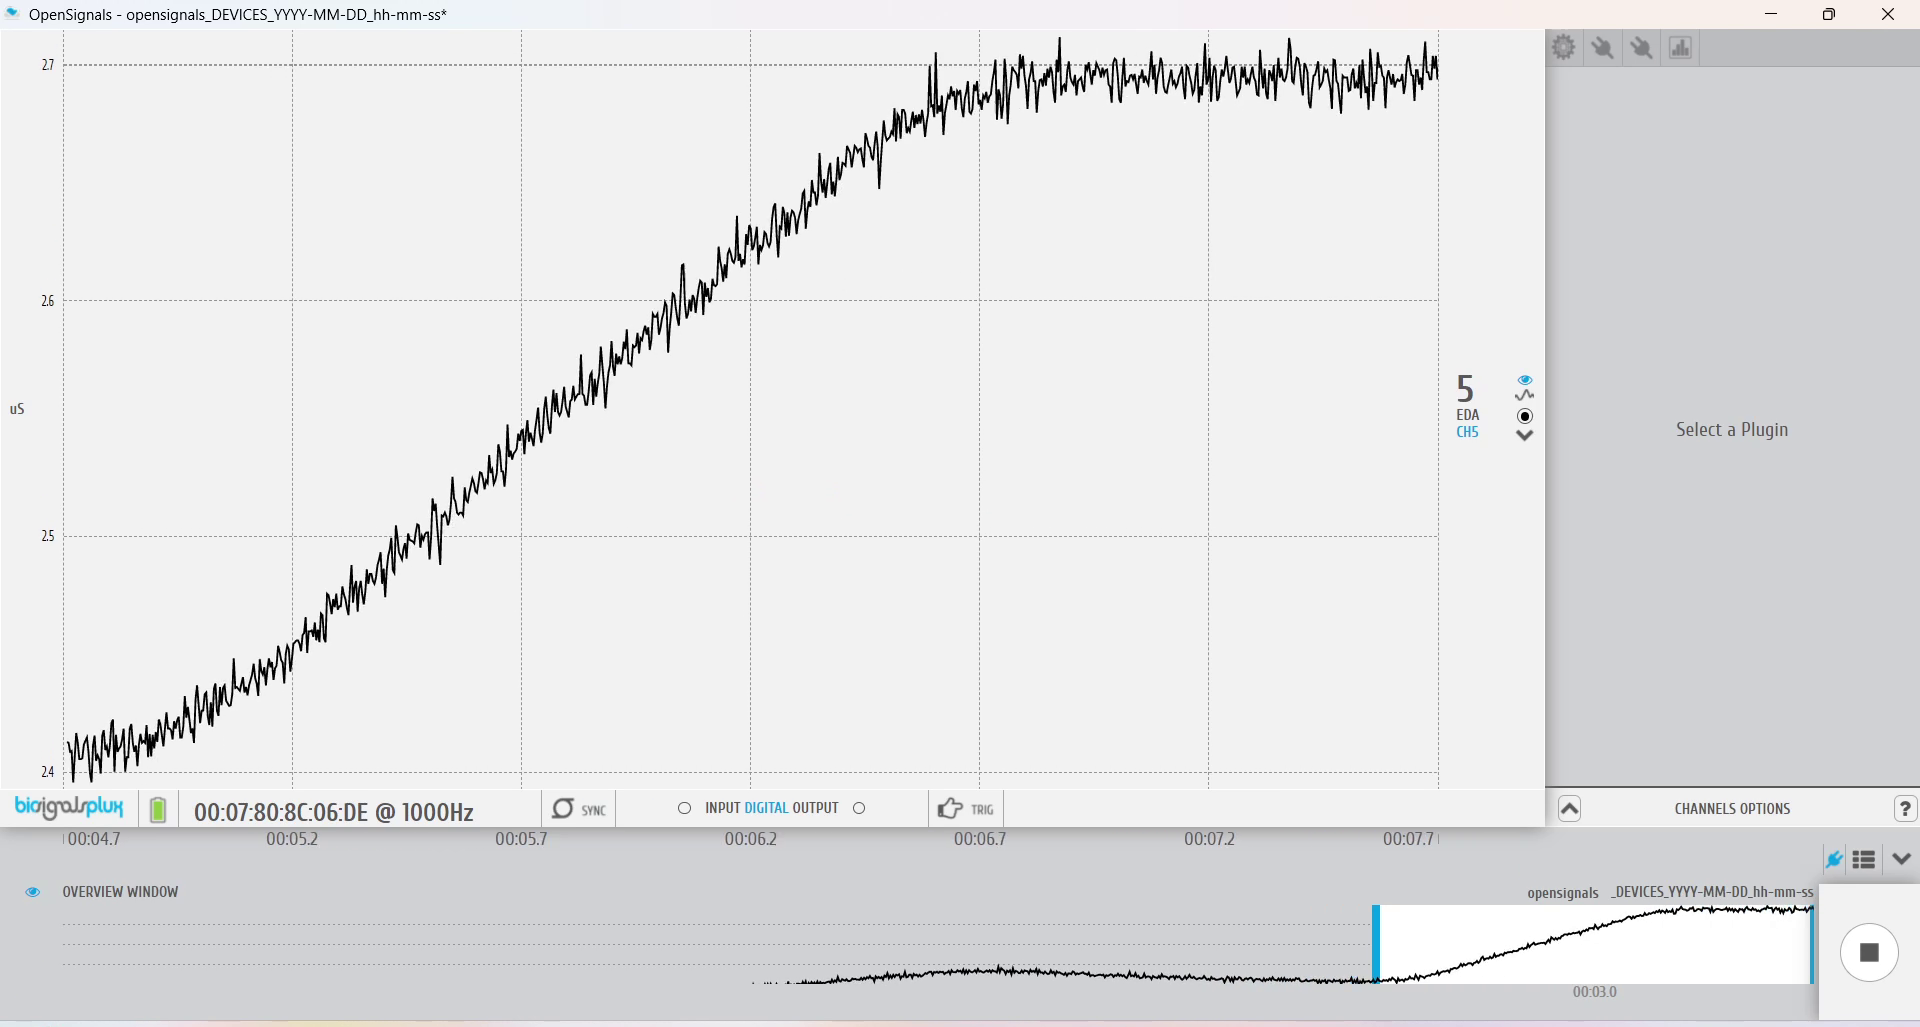
\includegraphics[height=0.34\textheight,max width=\linewidth,keepaspectratio]{media/media/image21.png}\end{center}

\phantomsection\addcontentsline{lof}{figure}{\protect\numberline{A.9}OpenSignals Recording Screen.}%
\textbf{Figure A.9} OpenSignals Recording Screen . The user is shown a live waveform view with a time timeline while the recording is being conducted. The waveform view is customisable (zoom in/zoom out) and user can halt the recording by clicking on the stop button on bottom right.
\end{figure}

\vspace{1.5em}


\begin{figure}[H]
\begin{center}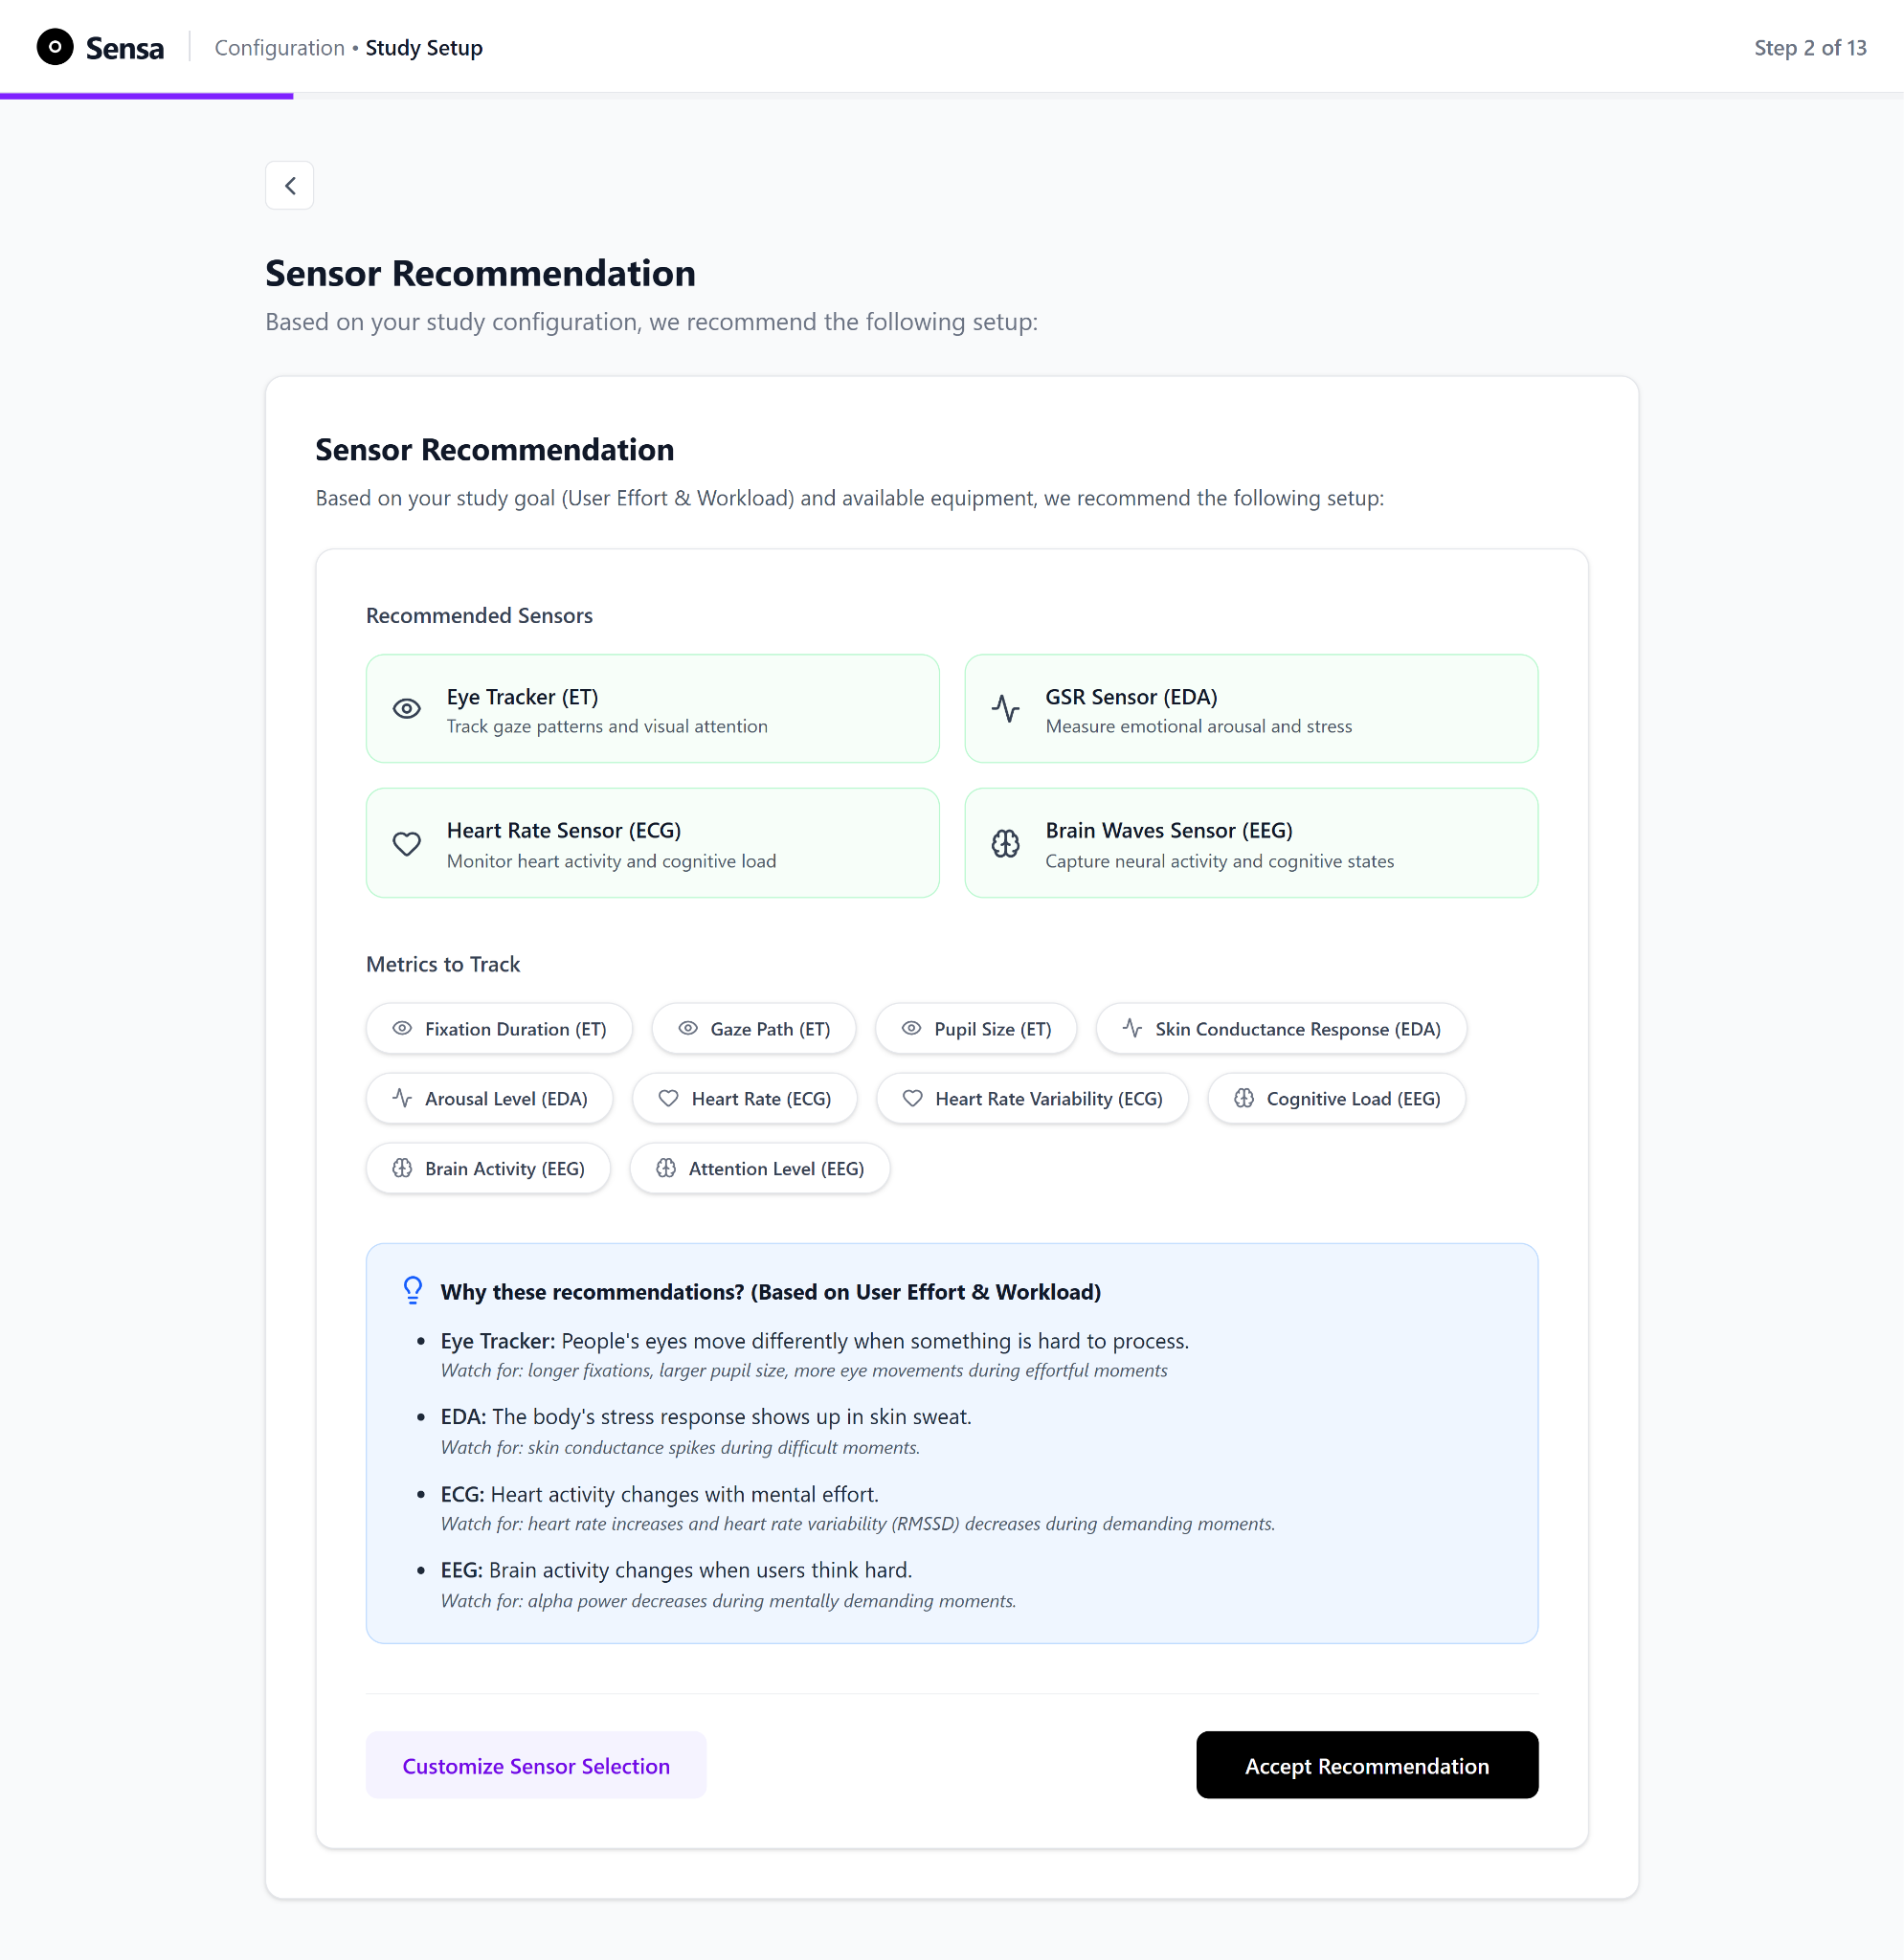
\includegraphics[height=0.34\textheight,max width=\linewidth,keepaspectratio]{media/media/image2.png}\end{center}

\phantomsection\addcontentsline{lof}{figure}{\protect\numberline{A.10}OpenSignals Save modal.}%
\textbf{Figure A.10} OpenSignals Save modal . The user is shown a popup modal which allows them to rename the file, select its save location, change the extension and add description.
\end{figure}

\vspace{1.5em}


\begin{figure}[H]
\begin{center}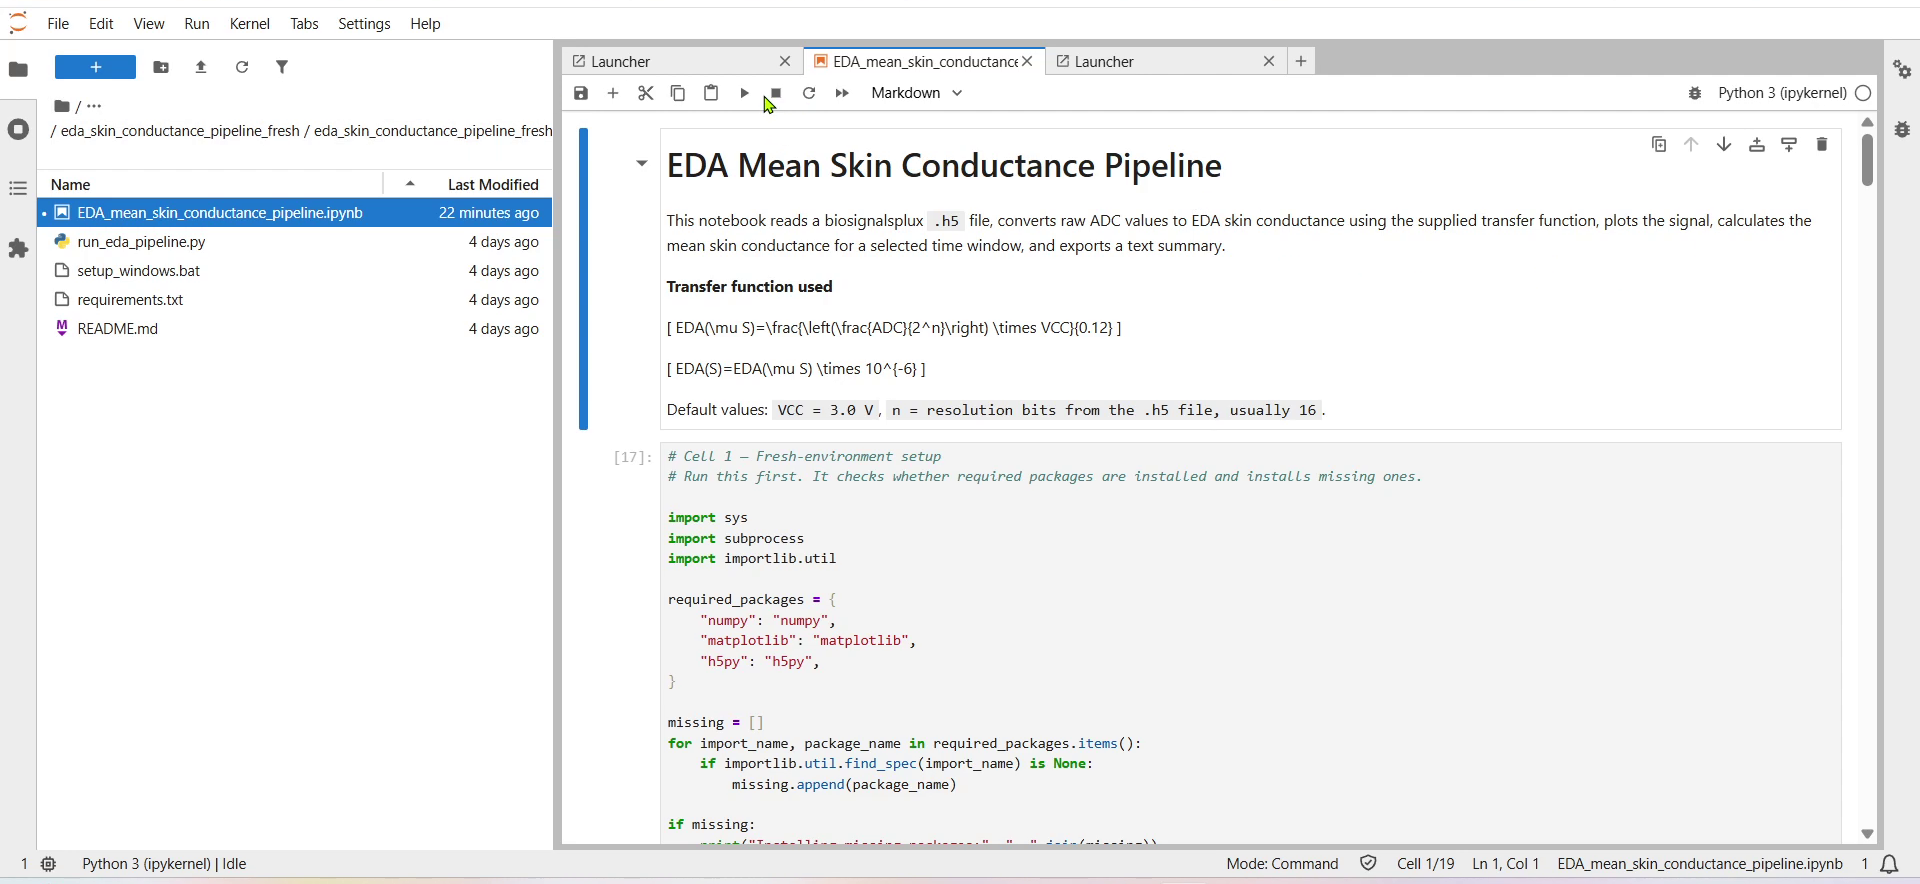
\includegraphics[height=0.34\textheight,max width=\linewidth,keepaspectratio]{media/media/image33.png}\end{center}

\phantomsection\addcontentsline{lof}{figure}{\protect\numberline{A.11}JupyterLab with Mean EDA Skin Conductance Pipeline.}%
\textbf{Figure A.11} JupyterLab with Mean EDA Skin Conductance Pipeline. The user is shown a script with instructions on how to run it. Pressing the `play' button executes one chunk of the script.
\end{figure}

\vspace{1.5em}


\begin{figure}[H]
\begin{center}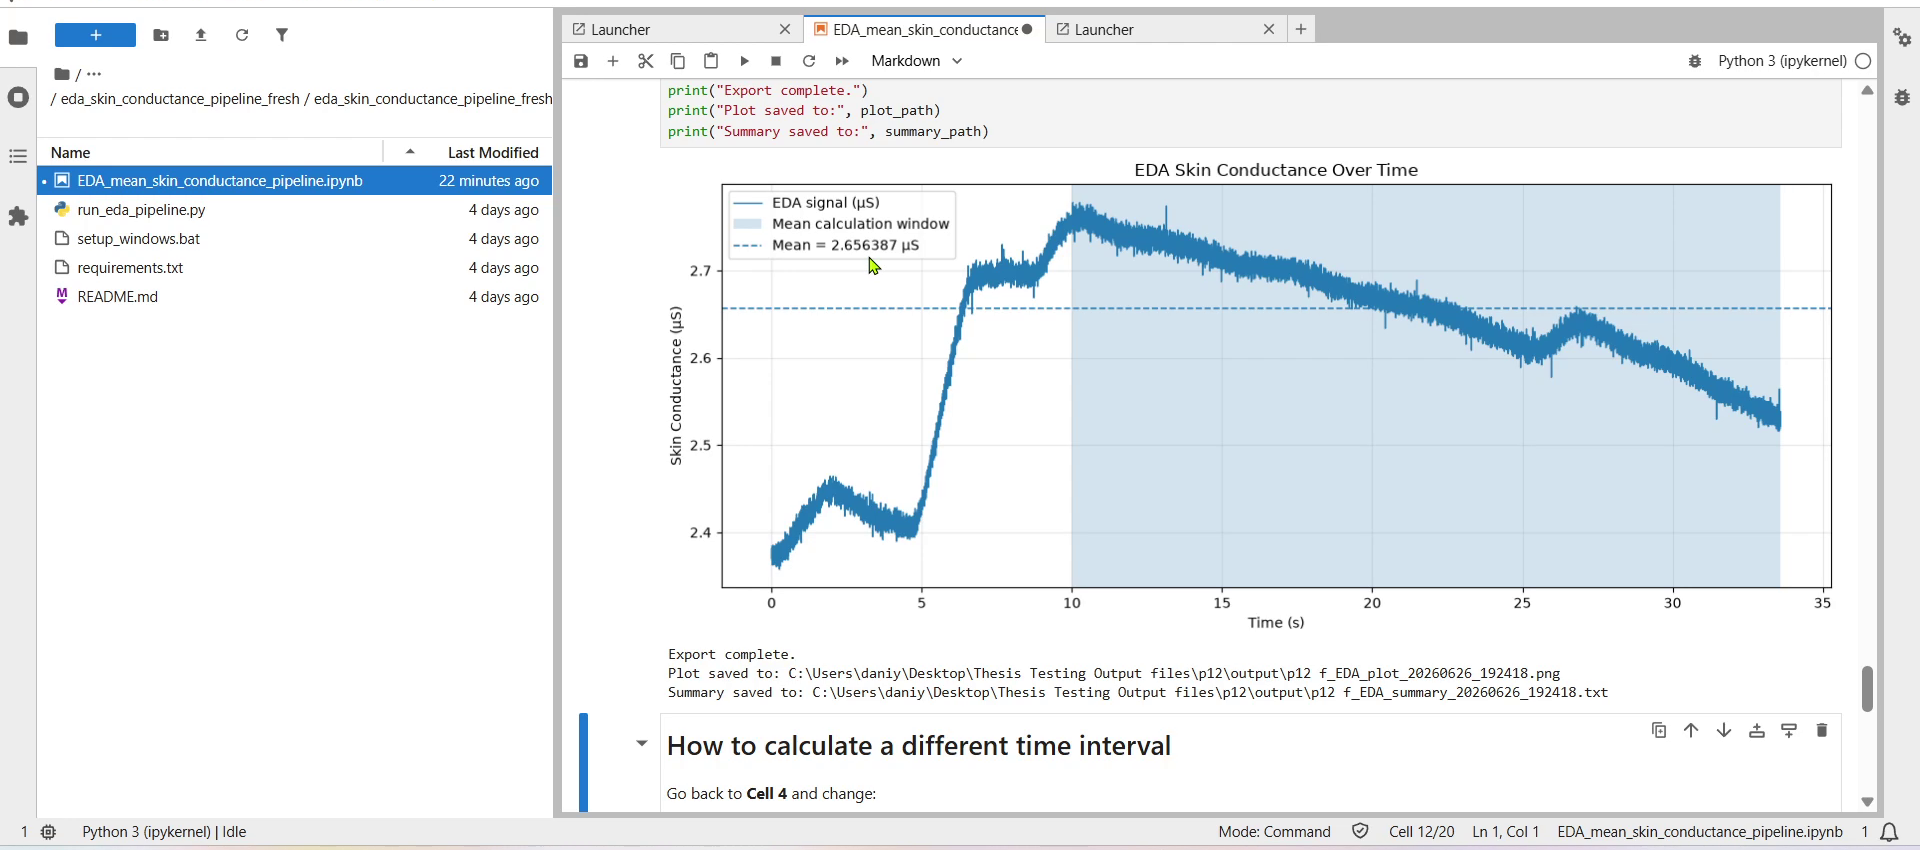
\includegraphics[height=0.34\textheight,max width=\linewidth,keepaspectratio]{media/media/image19.png}\end{center}

\phantomsection\addcontentsline{lof}{figure}{\protect\numberline{A.12}JupyterLab with computed Mean EDA.}%
\textbf{Figure A.12} JupyterLab with computed Mean EDA. After running the script, the user is shown a skin conductance over time graph. This is accompanied by the computed Mean EDA value, utilizing a transfer function.
\end{figure}

\vspace{1.5em}


\clearpage
\clearpage
\hypertarget{appendix-a1-task-prompt-fragmented-workflow}{%
\subsection{Appendix B1: Task Prompt (Fragmented Workflow)}\label{appendix-a1-task-prompt-fragmented-workflow}}

This is the printed task prompt given to participants in the fragmented condition. Participants self-administered the condition by working through this prompt, which directed them to Tobii Eye Tracking Core, OpenSignals, and the Jupyter validation script in sequence. It is reproduced as participants received it.

\textbf{Task Prompt: Fragmented Workflow\\
(Tobii Eye Tracking Core + OpenSignals)}

\textbf{Scenario}

You are a research assistant preparing to run a short physiological study session. Before you can begin recording data, you need to calibrate an eye tracker and verify your skin-conductance (EDA) sensor. You have two separate, standalone tools available: Tobii Core for the eye tracker, and OpenSignals for the EDA sensor. There is no unified interface connecting the two. Please follow the steps below using the available tools and the printed reference sheets and user manual extracts provided.

\emph{You are \textbf{not being evaluated on your personal performance}. We are interested in how the tools support (or do not support) this task.}

\textbf{Important}

\begin{itemize}
\item
  Work through the steps at your own pace.
\item
  The researcher will not assist you during the task, unless you ask for a clarification or there's a critical breakdown.
\item
  There are no right or wrong answers. We are evaluating the tools, not you.
\item
  If you are unsure how to proceed, do your best and continue.
\end{itemize}

\textbf{Your Task:}

\textbf{Step 1: Study documentation}

\Needspace{23\baselineskip}
Open the provided Google Docs template and record the following study parameters manually. For fields not mentioned:

\begingroup\renewcommand{\longtablestretch}{1.6}
\begin{longtable}[]{@{}
  >{\raggedright\arraybackslash}p{(\columnwidth - 2\tabcolsep) * \real{0.3369}}
  >{\raggedright\arraybackslash}p{(\columnwidth - 2\tabcolsep) * \real{0.6431}}@{}}
\toprule\noalign{}
\begin{minipage}[t]{\linewidth}\raggedright
\textbf{Study Name}
\end{minipage} & \begin{minipage}[t]{\linewidth}\raggedright
Checkout Flow Usability Study
\end{minipage} \\
\begin{minipage}[t]{\linewidth}\raggedright
\textbf{Study Goal}
\end{minipage} & \begin{minipage}[t]{\linewidth}\raggedright
Measure User Effort and Workload
\end{minipage} \\
\begin{minipage}[t]{\linewidth}\raggedright
\textbf{Study Type}
\end{minipage} & \begin{minipage}[t]{\linewidth}\raggedright
Web Based Usability Study
\end{minipage} \\
\begin{minipage}[t]{\linewidth}\raggedright
\textbf{Interface Type}
\end{minipage} & \begin{minipage}[t]{\linewidth}\raggedright
Web application
\end{minipage} \\
\begin{minipage}[t]{\linewidth}\raggedright
\textbf{Test Environment}
\end{minipage} & \begin{minipage}[t]{\linewidth}\raggedright
Lab
\end{minipage} \\
\begin{minipage}[t]{\linewidth}\raggedright
\textbf{Sensors to use}
\end{minipage} & \begin{minipage}[t]{\linewidth}\raggedright
Eye Tracker, ECG, EEG, EDA
\end{minipage} \\
\begin{minipage}[t]{\linewidth}\raggedright
\textbf{Project Name}
\end{minipage} & \begin{minipage}[t]{\linewidth}\raggedright
Test Project for Participant ID: {[}enter participant id{]}
\end{minipage} \\
\begin{minipage}[t]{\linewidth}\raggedright
\textbf{Number of participants}
\end{minipage} & \begin{minipage}[t]{\linewidth}\raggedright
1
\end{minipage} \\
\begin{minipage}[t]{\linewidth}\raggedright
\textbf{Project objectives}
\end{minipage} & \begin{minipage}[t]{\linewidth}\raggedright
Identify usability issues in the checkout flow and measure participant cognitive and emotional responses
\end{minipage} \\
\begin{minipage}[t]{\linewidth}\raggedright
\textbf{Project description (optional)}
\end{minipage} & \begin{minipage}[t]{\linewidth}\raggedright
We will conduct usability tests with participants to identify pain points and measure engagement throughout the checkout process for the checkout feature.
\end{minipage} \\
\midrule\noalign{}
\endhead
\bottomrule\noalign{}
\endlastfoot
\end{longtable}
\endgroup

\textbf{Step 2: Eye-tracking calibration}

\begin{enumerate}
\def\labelenumi{\arabic{enumi}.}
\item
  Open Tobii Core.
\item
  Position yourself at the standard viewing distance of 60 cm from the screen-mounted eye tracker.
\item
  Follow the on-screen instructions to complete the point-based calibration sequence.
\item
  Confirm that the calibration has completed.
\item
  Confirm the calibration result by performing a validation check using Tobii Core.
\end{enumerate}

\textbf{Step 3: EDA sensor setup and baseline recording}

\begin{enumerate}
\def\labelenumi{\arabic{enumi}.}
\item
  Refer to the printed reference sheet for electrode placement instructions.
\item
  Place the EDA electrode on your own hand as shown on the reference sheet.
\item
  Connect the Biosignalsplux hub via Bluetooth.
\item
  Open OpenSignals.
\item
  Confirm that a live waveform is visible (not flat-lined) and that the signal looks reasonably stable.
\item
  Sit still and breathe normally.
\item
  Record a 30-second resting baseline.
\item
  Save and export the recording as a .h5 file in the format: PartipantID.h5 (\emph{Example: p01.h5)}
\end{enumerate}

\textbf{Step 4: Compute the baseline value}

\begin{enumerate}
\def\labelenumi{\arabic{enumi}.}
\item
  Open Jupyter Lab.
\item
  Run the provided script on your exported .h5 file.
\item
  Refer to the provided read me file on instructions on how to use the script, if needed.
\item
  Note and report the mean EDA value (in microsiemens) reported by the script.
\end{enumerate}

\textbf{Notify the researcher when the Eye Tracker and EDA sensors are calibrated and you are satisfied that the system is ready to begin recording. This marks the completion of your task.}

\clearpage
\hypertarget{appendix-a2-task-prompt-unified-workflow}{%
\subsection{Appendix B2: Task Prompt (Unified Workflow)}\label{appendix-a2-task-prompt-unified-workflow}}

This is the printed task prompt given to participants in the unified condition, directing them through the Sensa onboarding and calibration workflow. It is reproduced as participants received it.

\textbf{Task Prompt, Unified Workflow (Sensa)}

\textbf{Scenario}

You are a research assistant preparing to run a short physiological study session. Before you can begin recording data, you need to calibrate an eye tracker and verify your skin-conductance (EDA) sensor. You have a single unified platform, Sensa, that guides you through study setup, sensor selection, readiness checks, and calibration for both devices. Please follow the on-screen guidance provided by Sensa.

\emph{You are \textbf{not being evaluated on your personal performance}. We are interested in how the tools support (or do not support) this task.}

\textbf{Important}

\begin{itemize}
\item
  Work through the steps at your own pace.
\item
  The researcher will not assist you during the task, unless you ask for a clarification or there's a critical breakdown.
\item
  There are no right or wrong answers. We are evaluating the tools, not you.
\item
  If you are unsure how to proceed, do your best and continue.
\end{itemize}

\textbf{Your Task:}

Using Sensa, complete the full study setup and sensor calibration process so that you are ready to begin recording.

\textbf{Step 1: Study setup}

\begin{enumerate}
\def\labelenumi{\arabic{enumi}.}
\item
  Open Sensa.
\item
  Follow the onboarding flow to define the study goal, interface type, and test environment.
\item
  Select the available hardware and the sensors you will use for this session.
\item
  Use the following parameters to set up your study:
\end{enumerate}

\Needspace{20\baselineskip}
\begingroup\renewcommand{\longtablestretch}{1.6}
\begin{longtable}[]{@{}
  >{\raggedright\arraybackslash}p{(\columnwidth - 2\tabcolsep) * \real{0.3369}}
  >{\raggedright\arraybackslash}p{(\columnwidth - 2\tabcolsep) * \real{0.6431}}@{}}
\toprule\noalign{}
\begin{minipage}[t]{\linewidth}\raggedright
\textbf{Study Name}
\end{minipage} & \begin{minipage}[t]{\linewidth}\raggedright
Checkout Flow Usability Study
\end{minipage} \\
\begin{minipage}[t]{\linewidth}\raggedright
\textbf{Study Goal}
\end{minipage} & \begin{minipage}[t]{\linewidth}\raggedright
Measure User Effort and Workload
\end{minipage} \\
\begin{minipage}[t]{\linewidth}\raggedright
\textbf{Study Type}
\end{minipage} & \begin{minipage}[t]{\linewidth}\raggedright
Web Based Usability Study
\end{minipage} \\
\begin{minipage}[t]{\linewidth}\raggedright
\textbf{Interface Type}
\end{minipage} & \begin{minipage}[t]{\linewidth}\raggedright
Web application
\end{minipage} \\
\begin{minipage}[t]{\linewidth}\raggedright
\textbf{Test Environment}
\end{minipage} & \begin{minipage}[t]{\linewidth}\raggedright
Lab
\end{minipage} \\
\begin{minipage}[t]{\linewidth}\raggedright
\textbf{Sensors to use}
\end{minipage} & \begin{minipage}[t]{\linewidth}\raggedright
Eye Tracker, ECG, EEG, EDA
\end{minipage} \\
\begin{minipage}[t]{\linewidth}\raggedright
\textbf{Project Name}
\end{minipage} & \begin{minipage}[t]{\linewidth}\raggedright
Test Project for Participant ID: {[}enter participant id{]}
\end{minipage} \\
\begin{minipage}[t]{\linewidth}\raggedright
\textbf{Number of participants}
\end{minipage} & \begin{minipage}[t]{\linewidth}\raggedright
1
\end{minipage} \\
\begin{minipage}[t]{\linewidth}\raggedright
\textbf{Project objectives}
\end{minipage} & \begin{minipage}[t]{\linewidth}\raggedright
Identify usability issues in the checkout flow and measure participant cogn i itive and emotional responses
\end{minipage} \\
\begin{minipage}[t]{\linewidth}\raggedright
\textbf{Project description (optional)}
\end{minipage} & \begin{minipage}[t]{\linewidth}\raggedright
We will conduct usability tests with participants to identify pain points and measure engagement throughout the checkout process for the checkout feature.
\end{minipage} \\
\midrule\noalign{}
\endhead
\bottomrule\noalign{}
\endlastfoot
\end{longtable}
\endgroup

\textbf{Step 2: Readiness check}

Follow Sensa\textquotesingle s readiness checklist and confirm all items before proceeding to calibration.

\textbf{Step 3: Eye-tracking calibration}

\begin{enumerate}
\def\labelenumi{\arabic{enumi}.}
\item
  Follow Sensa\textquotesingle s guided calibration flow for the eye tracker.
\item
  Position yourself as instructed by the on-screen guidance.
\item
  Complete the calibration sequence.
\item
  Confirm the calibration result by performing a validation check using Sensa.
\end{enumerate}

\textbf{Step 4: EDA sensor calibration and baseline recording}

\begin{enumerate}
\def\labelenumi{\arabic{enumi}.}
\item
  Follow Sensa\textquotesingle s guided flow to place the EDA electrode on your own hand.
\item
  Confirm the signal quality check shown by Sensa.
\item
  Sit still and breathe normally while Sensa records a 30-second resting baseline.
\item
  Note the mean EDA value (in microsiemens) shown by Sensa.
\end{enumerate}

\textbf{Notify the researcher when the Eye Tracker and EDA sensors are calibrated and you are satisfied that the system is ready to begin recording. This marks the completion of your task.}

\clearpage
\hypertarget{appendix-b-participant-intake-form}{%
\subsection{\texorpdfstring{Appendix C: Participant Intake Form }{Appendix C: Participant Intake Form }}\label{appendix-b-participant-intake-form}}

The following intake form was administered to all participants via Google Forms before their study session. It captured contact details, demographic information, prior experience with the relevant technologies, and scheduling availability. Required questions are marked with an asterisk (*).

\textbf{1. Full Name} * Short answer.

\textbf{2. Email address} * Short answer.

\textbf{3. WhatsApp (Optional)} If you prefer to be contacted via phone. Short answer.

\textbf{4. Age} * Multiple choice (single selection):

\begin{itemize}
\item
  18 to 24
\item
  25 to 34
\item
  35 to 44
\item
  45 to 54
\item
  55+
\end{itemize}

\textbf{5. Current status / role} * Multiple choice (single selection):

\begin{itemize}
\item
  Bachelor\textquotesingle s Student
\item
  Master\textquotesingle s Student
\item
  PhD student / research assistant
\item
  Faculty / staff
\item
  Other: (free text)
\end{itemize}

\textbf{6. Study programme or field} * e.g. Usability Engineering, Computer Science, Psychology, etc. Short answer.

\textbf{7. Do you use a desktop or laptop computer regularly for work or study?} * Multiple choice (single selection):

\begin{itemize}
\item
  Yes
\item
  No
\end{itemize}

\textbf{8. Have you previously used eye-tracking software or hardware? (for example, Tobii Eyetrackers or similar)} * Note: The answer does not affect your participation in this study. Multiple choice (single selection):

\begin{itemize}
\item
  Yes
\item
  No
\end{itemize}

\textbf{9. Have you previously placed biosignal electrodes (for example, EEG, EDA/GSR, or ECG sensors) on yourself or another person?} * Note: The answer does not affect your participation in this study. Multiple choice (single selection):

\begin{itemize}
\item
  Yes
\item
  No
\end{itemize}

\textbf{10. General availability (Time)} * Note: The answer does not affect your participation in this study. Checkboxes (multiple selection):

\begin{itemize}
\item
  Weekday mornings (09:00 to 12:00)
\item
  Weekday afternoons (12:00 to 15:00)
\item
  Weekday evenings (15:00 to 18:00)
\item
  Other: (free text)
\end{itemize}

\textbf{11. General availability (Date)} * Note: The answer does not affect your participation in this study. Checkboxes (multiple selection):

\begin{itemize}
\item
  23 June 2026
\item
  24 June 2026
\item
  25 June 2026
\item
  26 June 2026
\item
  30 June 2026
\item
  1 July 2026
\item
  Other: (free text)
\end{itemize}



\clearpage
\hypertarget{appendix-c-participant-information-sheet}{%
\subsection{Appendix D: Participant Information Sheet}\label{appendix-c-participant-information-sheet}}

This is the information sheet given to each participant on arrival, describing the purpose of the study, what participation involved, and how data would be handled.

\noindent\rule{\linewidth}{0.4pt}

\textbf{Participant Information Sheet}

\textbf{Study title:} Designing and Evaluating Usability-Centred Onboarding and Calibration Workflows in Multi-Modal Research Platforms

\textbf{Researcher:} Daniyal (DA 35795), MSc Usability Engineering, Rhine-Waal University of Applied Sciences (HSRW)

\textbf{Supervisor:} Prof. Dr. Kai Essig

\noindent\rule{\linewidth}{0.4pt}

\textbf{What is this study about?}

This study investigates how researchers experience two different ways of preparing eye-tracking and physiological sensor equipment before a research session.

You will be asked to complete the same calibration task twice, using a different set of tools each. No prior experience with eye-tracking or biosignal equipment is required.

\textbf{Background: the equipment you will use}

\textbf{Eye tracker.} A screen-mounted device that uses infrared light to track where you are looking. It is non-contact and does not record images of you. It requires a short calibration (following a few points on screen) so it can map your gaze accurately. Running this calibration is part of your task.

\textbf{EDA sensor (electrodermal activity).} A skin-conductance sensor that measures small changes in the skin\textquotesingle s electrical conductance, which vary with physiological arousal. It is a standard research sensor, non-invasive, and passive: it reads from the skin surface and does not pass any current into the body. You will attach it to your own hand, sit still for a 30-second baseline recording, and that completes the measurement.

\textbf{What will you do?}

You will complete the same calibration task twice: once with each workflow. The order in which you complete the two workflows is assigned in advance and counterbalanced across participants, so you may complete either workflow first.

In each workflow, you will calibrate an eye tracker on yourself and record a short resting baseline using a skin-conductance (EDA) sensor attached to your own hand. During the task, the researcher may take written observation notes.

After each task, you will complete short questionnaires about your experience. At the end of the session, you will be asked to fill out a written questionnaire comparing the two workflows.

The total study duration is approximately 30 to 45 minutes, including a short break between the two workflows.

\textbf{Is participation voluntary?}

Yes. Participation is completely voluntary.

You may stop participating at any time without giving a reason. If you choose to withdraw, your data will not be used in the study.

\textbf{Are there any risks?}

This study involves minimal risk. Some participants may experience mild frustration, confusion or fatigue while completing the tasks. The EDA sensor is a non-invasive electrode placed on the skin and does not deliver any electrical stimulation. The eye tracker in a non-invasive hardware peripheral mounted on the desktop peripheral which records your gaze coordinates without providing any stimulation.

\textbf{Will your data be kept confidential?}

All collected data will be anonymised. Participants will be assigned a participant number, and no names will appear in the thesis or in any publication.

Anonymised data will be securely stored for academic research purposes and handled in accordance with GDPR data protection requirements.

\textbf{Will you be recorded?}

With your consent, your screen and task session may be recorded. The researcher may also take written observation notes during the session. No audio or video of your face or voice is required for this study unless separately agreed with you. A session may involve photography or videomaking during the experiment for documentation purposes with prior consent.

\textbf{Who can I contact with questions?}

You may contact the researcher (Daniyal Admany, 35795) or the thesis supervisor (Prof. Dr. Kai Essig, Rhine-Waal University of Applied Sciences) with any questions about this study, before, during, or after your participation.

\clearpage
\hypertarget{appendix-d-informed-consent-form}{%
\subsection{Appendix E: Informed Consent Form}\label{appendix-d-informed-consent-form}}

This is the consent form each participant read and signed before the session began.

\noindent\rule{\linewidth}{0.4pt}

\textbf{Informed Consent Form}

\textbf{Study title:} Designing and Evaluating Usability-Centred Onboarding and Calibration Workflows in Multi-Modal Research Platforms

\textbf{Researcher:} Daniyal (DA 35795), MSc Usability Engineering, Rhine-Waal University of Applied Sciences (HSRW)

\textbf{Supervisor:} Prof. Dr. Kai Essig

\noindent\rule{\linewidth}{0.4pt}

Participant Name: \_\_\_\_\_\_\_\_\_\_\_\_\_\_\_\_\_\_\_\_\_\_\_\_\_\_\_\_\_\_\_

Participant ID: \_\_\_\_\_\_\_\_\_\_\_\_\_\_\_\_\_\_\_\_\_\_\_\_\_\_\_\_\_\_\_

\emph{Please read each statement carefully and sign the consent form if you agree. If you have any questions before signing, please ask the researcher.}

\textbf{Statements}

\begin{enumerate}
\def\labelenumi{\arabic{enumi}.}
\item
  I have read and understood the Participant Information Sheet for this study.
\item
  I have had the opportunity to ask questions about the study and have received satisfactory answers.
\item
  I understand that my participation is voluntary and that I may withdraw at any time, without giving a reason, and without any consequence.
\item
  I understand that if I withdraw, my data will not be used in the study.
\item
  I understand that I will complete two calibration tasks (using two different workflows), each followed by short questionnaires, and a short interview at the end.
\item
  I understand that the researcher may take written observation notes during my session.
\item
  I understand that my data will be anonymised and that no names will appear in the thesis or any publication.
\item
  I understand that anonymised data will be stored securely for academic research purposes.
\end{enumerate}

\begin{quote}
\textbf{Recording consent (optional, tick the checkbox)}

\emph{You may decline any or all recording options below and still take part in the study.}
\end{quote}

\begin{enumerate}
\def\labelenumi{\arabic{enumi}.}
\setcounter{enumi}{8}
\item
  I consent to my screen activity being recorded during the task. \textbf{☐}
\item
  I consent to audio recording during the session. \textbf{☐}
\item
  I consent to video recording during the session. \textbf{☐}
\end{enumerate}

\textbf{Participant}

Date: \_\_\_\_\_\_\_\_\_\_\_\_\_\_\_\_\_\_\_\_\_\_\_\_\_\_\_\_\_\_\_

Signature: \_\_\_\_\_\_\_\_\_\_\_\_\_\_\_\_\_\_\_\_\_\_\_\_\_\_\_\_\_\_\_

\textbf{Researcher}

Name: Daniyal Admany

Date: \_\_\_\_\_\_\_\_\_\_\_\_\_\_\_\_\_\_\_\_\_\_\_\_\_\_\_\_\_\_\_

Signature: \_\_\_\_\_\_\_\_\_\_\_\_\_\_\_\_\_\_\_\_\_\_\_\_\_\_\_\_\_\_\_

\clearpage
\hypertarget{appendix-e-observation-and-breakdown-log-sheets}{%
\subsection{\texorpdfstring{Appendix F: Observation and Breakdown Log Sheets }{Appendix F: Observation and Breakdown Log Sheets }}\label{appendix-e-observation-and-breakdown-log-sheets}}

These are the per-condition log sheets used by the researcher to record interaction breakdowns during each session. Each of the five breakdown categories defined in Chapter 4.5.3 was tallied live as it occurred, together with free-text observation notes. The counts recorded here are the source of the interaction-breakdown results in Chapter 5.1.5, and the notes form part of the corpus for the thematic analysis.

\textbf{Session Observation Sheet (Fragmented)}

Participant ID\textbf{:} \_\_\_\_\_\_\_\_\_\_\_\_\_\_\_

Order (1st / 2nd condition completed): \_\_\_\_\_\_\_\_\_\_\_\_\_\_\_

Date: \_\_\_\_\_\_\_\_\_\_\_\_\_\_\_

Condition start time: \_\_\_\_\_\_\_\_\_\_\_\_\_\_\_ Condition end time: \_\_\_\_\_\_\_\_\_\_\_\_\_\_\_

Session start time: \_\_\_\_\_\_\_\_\_\_\_\_\_\_\_ Session end time: \_\_\_\_\_\_\_\_\_\_\_\_\_\_\_

Total session duration: \_\_\_\_\_\_\_\_\_\_\_\_\_\_\_\_\_

\textbf{Session Timestamps for condition:}

\Needspace{16\baselineskip}
\begin{longtable}[]{@{}
  >{\raggedright\arraybackslash}p{(\columnwidth - 2\tabcolsep) * \real{0.7400}}
  >{\raggedright\arraybackslash}p{(\columnwidth - 2\tabcolsep) * \real{0.2400}}@{}}
\toprule\noalign{}
\begin{minipage}[t]{\linewidth}\raggedright
\textbf{Event}
\end{minipage} & \begin{minipage}[t]{\linewidth}\raggedright
\textbf{Timestamp}
\end{minipage} \\
\begin{minipage}[t]{\linewidth}\raggedright
\end{minipage} & \begin{minipage}[t]{\linewidth}\raggedright
\end{minipage} \\
\begin{minipage}[t]{\linewidth}\raggedright
Study documentation started
\end{minipage} & \begin{minipage}[t]{\linewidth}\raggedright
\end{minipage} \\
\begin{minipage}[t]{\linewidth}\raggedright
Eye-tracking calibration started
\end{minipage} & \begin{minipage}[t]{\linewidth}\raggedright
\end{minipage} \\
\begin{minipage}[t]{\linewidth}\raggedright
Eye-tracking calibration completed
\end{minipage} & \begin{minipage}[t]{\linewidth}\raggedright
\end{minipage} \\
\begin{minipage}[t]{\linewidth}\raggedright
EDA setup started
\end{minipage} & \begin{minipage}[t]{\linewidth}\raggedright
\end{minipage} \\
\begin{minipage}[t]{\linewidth}\raggedright
EDA baseline recording started
\end{minipage} & \begin{minipage}[t]{\linewidth}\raggedright
\end{minipage} \\
\begin{minipage}[t]{\linewidth}\raggedright
EDA baseline recording completed
\end{minipage} & \begin{minipage}[t]{\linewidth}\raggedright
\end{minipage} \\
\begin{minipage}[t]{\linewidth}\raggedright
Task fully completed
\end{minipage} & \begin{minipage}[t]{\linewidth}\raggedright
\end{minipage} \\
\midrule\noalign{}
\endhead
\bottomrule\noalign{}
\endlastfoot
\end{longtable}

\textbf{Breakdown tally}

\Needspace{13\baselineskip}
Tally each occurrence as it happens. Total at the bottom of each row.

\begin{longtable}[]{@{}
  >{\raggedright\arraybackslash}p{(\columnwidth - 4\tabcolsep) * \real{0.7815}}
  >{\raggedright\arraybackslash}p{(\columnwidth - 4\tabcolsep) * \real{0.0992}}
  >{\raggedright\arraybackslash}p{(\columnwidth - 4\tabcolsep) * \real{0.0992}}@{}}
\toprule\noalign{}
\begin{minipage}[t]{\linewidth}\raggedright
\textbf{Breakdown type}
\end{minipage} & \begin{minipage}[t]{\linewidth}\raggedright
\textbf{Tally}
\end{minipage} & \begin{minipage}[t]{\linewidth}\raggedright
\textbf{Total}
\end{minipage} \\
\begin{minipage}[t]{\linewidth}\raggedright
Repeated calibration attempts (eye tracker)
\end{minipage} & \begin{minipage}[t]{\linewidth}\raggedright
\end{minipage} & \begin{minipage}[t]{\linewidth}\raggedright
\end{minipage} \\
\begin{minipage}[t]{\linewidth}\raggedright
Incorrect sequence execution
\end{minipage} & \begin{minipage}[t]{\linewidth}\raggedright
\end{minipage} & \begin{minipage}[t]{\linewidth}\raggedright
\end{minipage} \\
\begin{minipage}[t]{\linewidth}\raggedright
Repeated baseline recordings (EDA)
\end{minipage} & \begin{minipage}[t]{\linewidth}\raggedright
\end{minipage} & \begin{minipage}[t]{\linewidth}\raggedright
\end{minipage} \\
\begin{minipage}[t]{\linewidth}\raggedright
Hesitation periods (\textgreater5 sec inactivity during active calibration)
\end{minipage} & \begin{minipage}[t]{\linewidth}\raggedright
\end{minipage} & \begin{minipage}[t]{\linewidth}\raggedright
\end{minipage} \\
\begin{minipage}[t]{\linewidth}\raggedright
Requests for clarification
\end{minipage} & \begin{minipage}[t]{\linewidth}\raggedright
\end{minipage} & \begin{minipage}[t]{\linewidth}\raggedright
\end{minipage} \\
\midrule\noalign{}
\endhead
\bottomrule\noalign{}
\endlastfoot
\end{longtable}

\textbf{Total breakdown count (sum of all rows above): \_\_\_\_\_\_\_\_\_\_\_\_\_\_\_}

\textbf{Free-text notes and participant think aloud notes:}

\emph{(Time-stamp each note where possible, e.g. "02:34, hesitated before performing eyetracking calibration")}

\textbf{Researcher overall notes:}

\clearpage
\textbf{Session Observation Sheet (Unified)}

Participant ID\textbf{:} \_\_\_\_\_\_\_\_\_\_\_\_\_\_\_

Order (1st / 2nd condition completed): \_\_\_\_\_\_\_\_\_\_\_\_\_\_\_

Date: \_\_\_\_\_\_\_\_\_\_\_\_\_\_\_

Condition start time: \_\_\_\_\_\_\_\_\_\_\_\_\_\_\_ Condition end time: \_\_\_\_\_\_\_\_\_\_\_\_\_\_\_

Session start time: \_\_\_\_\_\_\_\_\_\_\_\_\_\_\_ Session end time: \_\_\_\_\_\_\_\_\_\_\_\_\_\_\_

Total session duration: \_\_\_\_\_\_\_\_\_\_\_\_\_\_\_\_\_

\textbf{Session Timestamps for condition:}

\Needspace{16\baselineskip}
\begin{longtable}[]{@{}
  >{\raggedright\arraybackslash}p{(\columnwidth - 2\tabcolsep) * \real{0.8241}}
  >{\raggedright\arraybackslash}p{(\columnwidth - 2\tabcolsep) * \real{0.1559}}@{}}
\toprule\noalign{}
\begin{minipage}[t]{\linewidth}\raggedright
\textbf{Event}
\end{minipage} & \begin{minipage}[t]{\linewidth}\raggedright
\textbf{Time}
\end{minipage} \\
\begin{minipage}[t]{\linewidth}\raggedright
Study setup started
\end{minipage} & \begin{minipage}[t]{\linewidth}\raggedright
\end{minipage} \\
\begin{minipage}[t]{\linewidth}\raggedright
Readiness check completed
\end{minipage} & \begin{minipage}[t]{\linewidth}\raggedright
\end{minipage} \\
\begin{minipage}[t]{\linewidth}\raggedright
Eye-tracking calibration started
\end{minipage} & \begin{minipage}[t]{\linewidth}\raggedright
\end{minipage} \\
\begin{minipage}[t]{\linewidth}\raggedright
Eye-tracking calibration completed
\end{minipage} & \begin{minipage}[t]{\linewidth}\raggedright
\end{minipage} \\
\begin{minipage}[t]{\linewidth}\raggedright
EDA setup started
\end{minipage} & \begin{minipage}[t]{\linewidth}\raggedright
\end{minipage} \\
\begin{minipage}[t]{\linewidth}\raggedright
EDA baseline recording started
\end{minipage} & \begin{minipage}[t]{\linewidth}\raggedright
\end{minipage} \\
\begin{minipage}[t]{\linewidth}\raggedright
EDA baseline recording completed
\end{minipage} & \begin{minipage}[t]{\linewidth}\raggedright
\end{minipage} \\
\begin{minipage}[t]{\linewidth}\raggedright
Task fully completed
\end{minipage} & \begin{minipage}[t]{\linewidth}\raggedright
\end{minipage} \\
\midrule\noalign{}
\endhead
\bottomrule\noalign{}
\endlastfoot
\end{longtable}

\textbf{First-pass calibration success (H5)}

\Needspace{7\baselineskip}
\begin{longtable}[]{@{}
  >{\raggedright\arraybackslash}p{(\columnwidth - 4\tabcolsep) * \real{0.8116}}
  >{\raggedright\arraybackslash}p{(\columnwidth - 4\tabcolsep) * \real{0.0919}}
  >{\raggedright\arraybackslash}p{(\columnwidth - 4\tabcolsep) * \real{0.0766}}@{}}
\toprule\noalign{}
\begin{minipage}[t]{\linewidth}\raggedright
\end{minipage} & \begin{minipage}[t]{\linewidth}\raggedright
\textbf{Yes}
\end{minipage} & \begin{minipage}[t]{\linewidth}\raggedright
\textbf{No}
\end{minipage} \\
\begin{minipage}[t]{\linewidth}\raggedright
Eye-tracking calibration accepted on first attempt
\end{minipage} & \begin{minipage}[t]{\linewidth}\raggedright
☐
\end{minipage} & \begin{minipage}[t]{\linewidth}\raggedright
☐
\end{minipage} \\
\midrule\noalign{}
\endhead
\bottomrule\noalign{}
\endlastfoot
\end{longtable}

Number of recalibration attempts (if any): \_\_\_\_\_\_\_\_\_\_\_\_\_\_\_

\textbf{Breakdown tally}

\Needspace{13\baselineskip}
Tally each occurrence as it happens. Total at the bottom of each row.

\begin{longtable}[]{@{}
  >{\raggedright\arraybackslash}p{(\columnwidth - 4\tabcolsep) * \real{0.7815}}
  >{\raggedright\arraybackslash}p{(\columnwidth - 4\tabcolsep) * \real{0.0992}}
  >{\raggedright\arraybackslash}p{(\columnwidth - 4\tabcolsep) * \real{0.0992}}@{}}
\toprule\noalign{}
\begin{minipage}[t]{\linewidth}\raggedright
\textbf{Breakdown type}
\end{minipage} & \begin{minipage}[t]{\linewidth}\raggedright
\textbf{Tally}
\end{minipage} & \begin{minipage}[t]{\linewidth}\raggedright
\textbf{Total}
\end{minipage} \\
\begin{minipage}[t]{\linewidth}\raggedright
Repeated calibration attempts
\end{minipage} & \begin{minipage}[t]{\linewidth}\raggedright
\end{minipage} & \begin{minipage}[t]{\linewidth}\raggedright
\end{minipage} \\
\begin{minipage}[t]{\linewidth}\raggedright
Incorrect sequence execution
\end{minipage} & \begin{minipage}[t]{\linewidth}\raggedright
\end{minipage} & \begin{minipage}[t]{\linewidth}\raggedright
\end{minipage} \\
\begin{minipage}[t]{\linewidth}\raggedright
Repeated baseline recordings (EDA)
\end{minipage} & \begin{minipage}[t]{\linewidth}\raggedright
\end{minipage} & \begin{minipage}[t]{\linewidth}\raggedright
\end{minipage} \\
\begin{minipage}[t]{\linewidth}\raggedright
Hesitation periods (\textgreater5 sec inactivity during active calibration)
\end{minipage} & \begin{minipage}[t]{\linewidth}\raggedright
\end{minipage} & \begin{minipage}[t]{\linewidth}\raggedright
\end{minipage} \\
\begin{minipage}[t]{\linewidth}\raggedright
Requests for clarification
\end{minipage} & \begin{minipage}[t]{\linewidth}\raggedright
\end{minipage} & \begin{minipage}[t]{\linewidth}\raggedright
\end{minipage} \\
\midrule\noalign{}
\endhead
\bottomrule\noalign{}
\endlastfoot
\end{longtable}

\textbf{Total breakdown count (sum of all rows above): \_\_\_\_\_\_\_\_\_\_\_\_\_\_\_}

\textbf{Captured values (recorded, not scored for H5 quality)}

\Needspace{10\baselineskip}
\begin{longtable}[]{@{}
  >{\raggedright\arraybackslash}p{(\columnwidth - 2\tabcolsep) * \real{0.8193}}
  >{\raggedright\arraybackslash}p{(\columnwidth - 2\tabcolsep) * \real{0.1607}}@{}}
\toprule\noalign{}
\begin{minipage}[t]{\linewidth}\raggedright
\textbf{Value}
\end{minipage} & \begin{minipage}[t]{\linewidth}\raggedright
\textbf{Reading}
\end{minipage} \\
\begin{minipage}[t]{\linewidth}\raggedright
Mean EDA baseline (microsiemens), shown by Sensa
\end{minipage} & \begin{minipage}[t]{\linewidth}\raggedright
\end{minipage} \\
\begin{minipage}[t]{\linewidth}\raggedright
Gaze accuracy (Sensa validation grid)
\end{minipage} & \begin{minipage}[t]{\linewidth}\raggedright
\end{minipage} \\
\begin{minipage}[t]{\linewidth}\raggedright
Gaze precision (Sensa validation grid)
\end{minipage} & \begin{minipage}[t]{\linewidth}\raggedright
\end{minipage} \\
\begin{minipage}[t]{\linewidth}\raggedright
Valid data yield (Sensa validation grid)
\end{minipage} & \begin{minipage}[t]{\linewidth}\raggedright
\end{minipage} \\
\midrule\noalign{}
\endhead
\bottomrule\noalign{}
\endlastfoot
\end{longtable}

\textbf{Free-text notes}

(Time-stamp each note where possible, e.g. "12:34 - hesitated before confirming readiness check")

\textbf{Researcher overall notes}

\clearpage
\hypertarget{appendix-f-post-task-open-questionnaire}{%
\subsection{Appendix G: Post-Task Open Questionnaire}\label{appendix-f-post-task-open-questionnaire}}

This is the open-response questionnaire administered immediately after each condition. Participants typed their answers directly into a Google Form. The open form targeted five themes: overall experience, ease of use, clarity of guidance, calibration confidence, and perceived workflow quality. The written responses collected here, together with the researcher observation notes, form the corpus for the reflexive thematic analysis reported in Chapter 5.2 and coded in full in Appendix L.

\textbf{Core Questions}

\textbf{1. Overall experience}

How did that go for you overall? How did it feel to work through the setup and calibration?

Further probe: Was there any part that stood out, positive or negative?

\textbf{2. Ease of use}

How easy or difficult was it to complete the setup and calibration? Were there any points where you felt stuck or unsure what to do?

Further probe: What made those moments difficult?

\textbf{3. Clarity of guidance}

Did the instructions and feedback give you enough information to know what to do at each step? Was there anywhere the guidance felt unclear or missing?

Further probe: What would have helped you at that point?

\textbf{4. Calibration confidence}

By the end, how confident were you that the sensors were properly calibrated and ready to record? What made you feel that way?

Further probe: Was there anything that made you doubt whether the setup was correct?

\textbf{5. Perceived workflow quality}

Thinking about the workflow as a whole, what worked well and what would you change? If you had to do this regularly, how would you feel about it?

Further probe: Was the order of steps logical to you? Did anything feel redundant or out of place?

\clearpage
\hypertarget{appendix-g-post-task-objective-questionnaires}{%
\subsection{\texorpdfstring{Appendix H: Post-Task Objective Questionnaires }{Appendix H: Post-Task Objective Questionnaires }}\label{appendix-g-post-task-objective-questionnaires}}

All post-task measures were administered via a single Google Form completed by each participant at the end of each condition. The form comprised three sections: the System Usability Scale (SUS), a Raw NASA-TLX, and a calibration confidence rating. This appendix reproduces the three validated or fixed instruments administered after each condition. Each is shown as presented to participants.

\hypertarget{section-1-system-usability-scale-sus}{%
\subsubsection{Section 1: System Usability Scale (SUS)}\label{section-1-system-usability-scale-sus}}

Participants rated their agreement with each statement on a 5-point scale (1 = Strongly disagree, 5 = Strongly agree). "The system" refers to the tools the participant used to complete the setup and calibration.

\begin{enumerate}
\def\labelenumi{\arabic{enumi}.}
\item
  I think that I would like to use this system frequently.
\item
  I found the system unnecessarily complex.
\item
  I thought the system was easy to use.
\item
  I think that I would need the support of a technical person to be able to use this system.
\item
  I found the various functions in this system were well integrated.
\item
  I thought there was too much inconsistency in this system.
\item
  I would imagine that most people would learn to use this system very quickly.
\item
  I found the system very cumbersome to use.
\item
  I felt very confident using the system.
\item
  I needed to learn a lot of things before I could get going with this system.
\end{enumerate}

\hypertarget{section-2-nasa-tlx-raw}{%
\subsubsection{Section 2: NASA-TLX (Raw)}\label{section-2-nasa-tlx-raw}}

Participants rated each of the six dimensions on a 0-10 linear scale. Endpoint anchors are shown in parentheses.

\begin{enumerate}
\def\labelenumi{\arabic{enumi}.}
\item
  Mental Demand: How mentally demanding was the task? (0 = Very Low, 10 = Very High)
\item
  Physical Demand: How physically demanding was the task? (0 = Very Low, 10 = Very High)
\item
  Temporal Demand: How hurried or rushed was the pace of the task? (0 = Very Low, 10 = Very High)
\item
  Performance: How successful were you in accomplishing what you were asked to do? (0 = Perfect, 10 = Failure)
\item
  Effort: How hard did you have to work to accomplish your level of performance? (0 = Very Low, 10 = Very High)
\item
  Frustration: How insecure, discouraged, irritated, stressed, and annoyed were you? (0 = Very Low, 10 = Very High)
\end{enumerate}

\hypertarget{section-3-calibration-confidence-rating}{%
\subsubsection{Section 3: Calibration Confidence Rating}\label{section-3-calibration-confidence-rating}}

Participants rated the following on a 7-point scale (1 = Not at all confident, 7 = Completely confident).

\begin{enumerate}
\def\labelenumi{\arabic{enumi}.}
\item
  How confident are you that the sensors were correctly calibrated and that the system was ready to record reliable data?
\item
  Briefly, what made you feel that way? (Optional follow-up, free text)
\end{enumerate}

\clearpage
\hypertarget{appendix-m}{%
\subsection{Appendix I: Google Doc Study Documentation template}\label{appendix-m}}

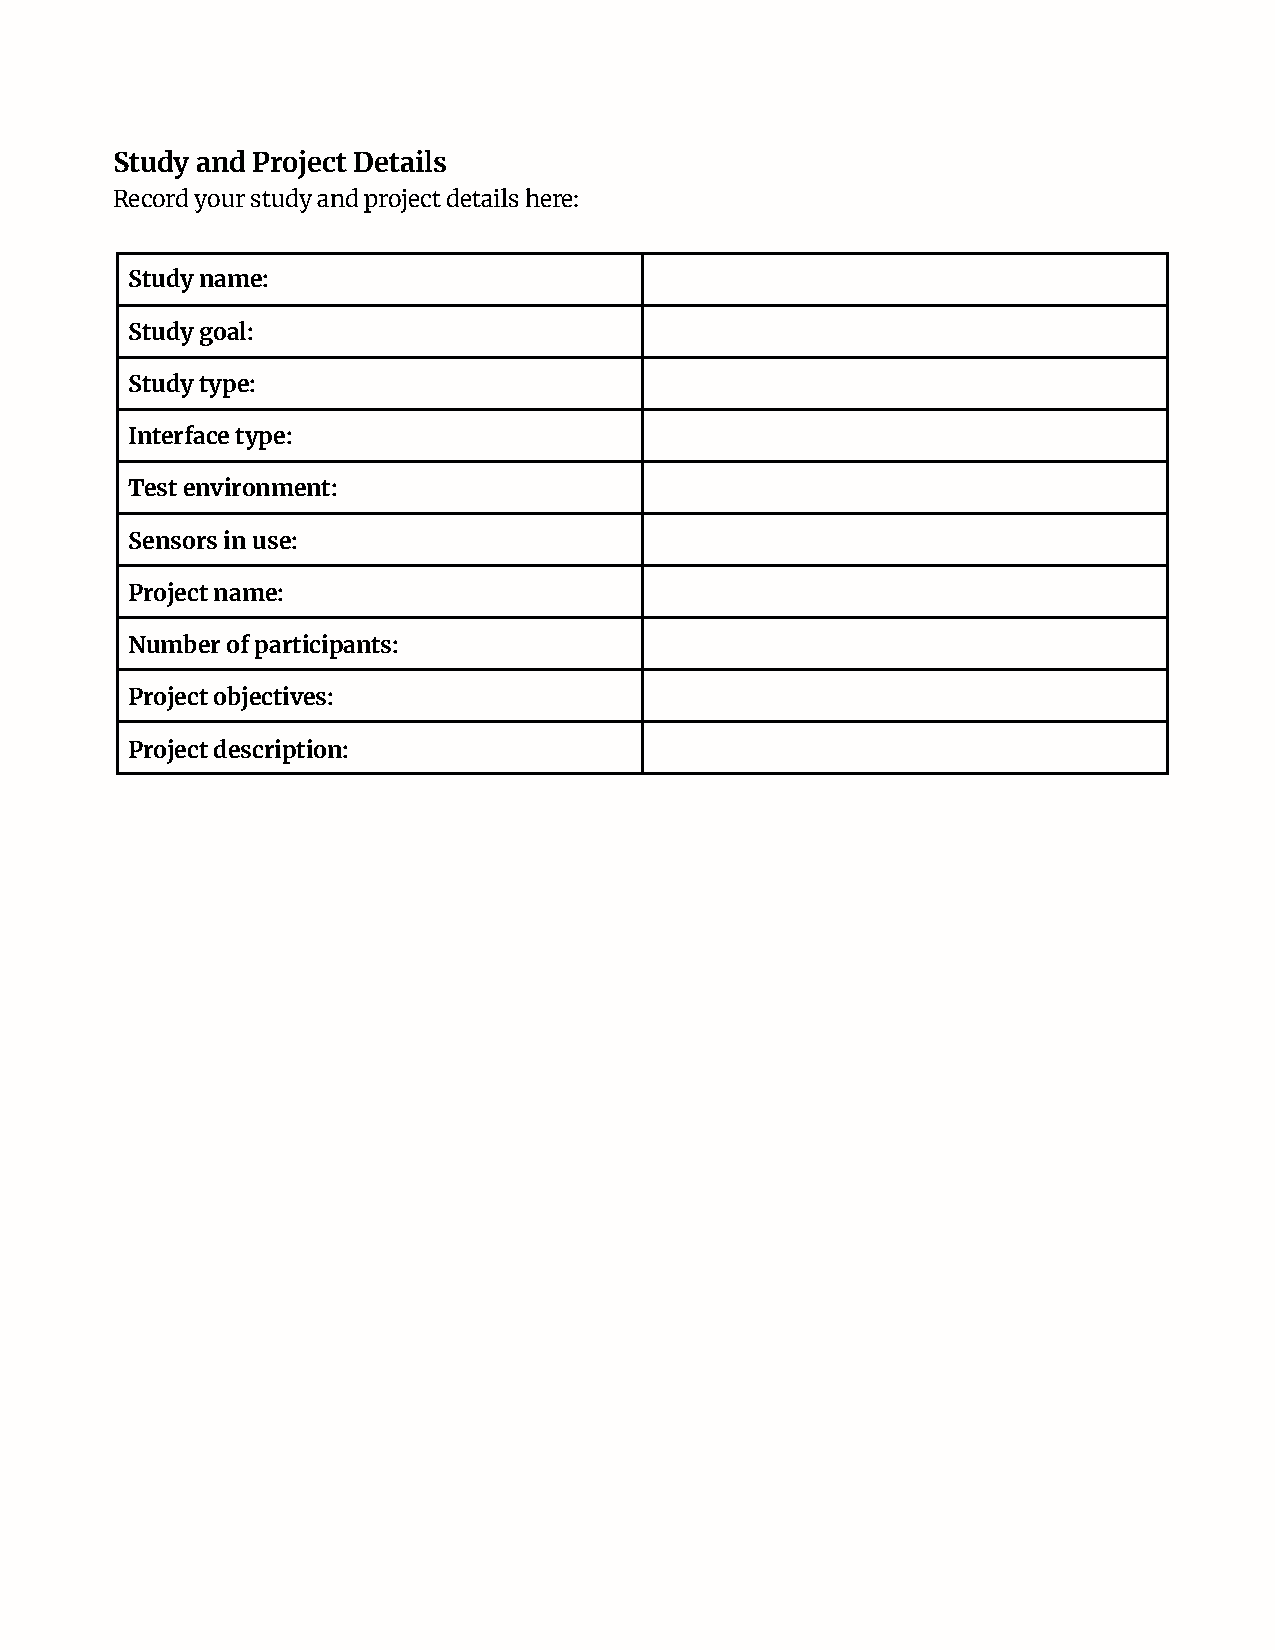
\includepdf[pages=-,width=\textwidth,pagecommand={}]{appendix/appendix-M.pdf}

\clearpage
\hypertarget{appendix-h-tobii-eye-tracking-software-manual-extract}{%
\subsection{\texorpdfstring{Appendix J: Tobii Eye Tracking Software Manual Extract }{Appendix J: Tobii Eye Tracking Software Manual Extract }}\label{appendix-h-tobii-eye-tracking-software-manual-extract}}

This is the printed reference extract available to participants during eye-tracker calibration in the fragmented condition. It documents the Tobii Eye Tracking software used to calibrate the eye tracker in this study. Reproduced from Dell Inc. (2016).

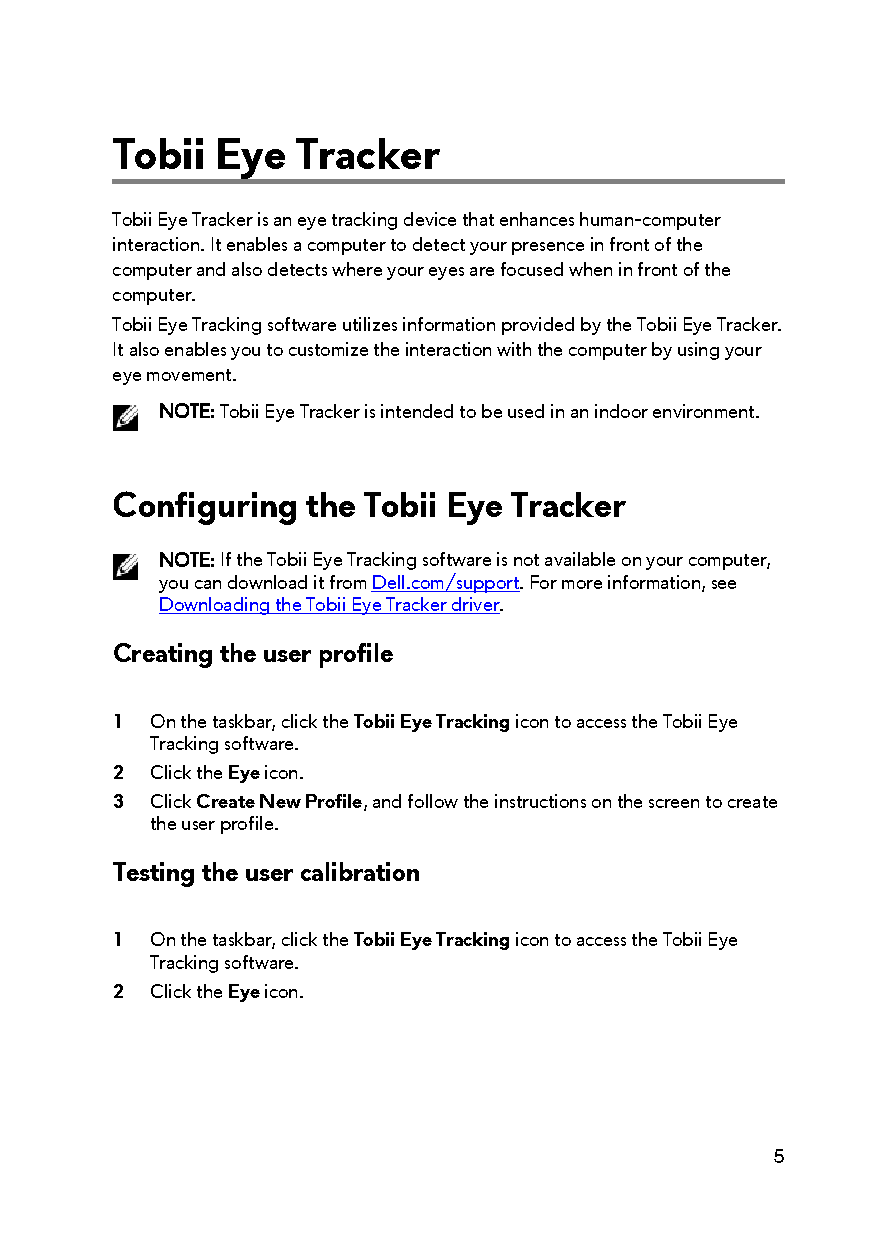
\includepdf[pages=-,width=\textwidth,pagecommand={}]{appendix/appendix-H.pdf}



\clearpage
\hypertarget{appendix-i-eda-sensor-reference-datasheet}{%
\subsection{Appendix K: EDA Sensor Reference Datasheet}\label{appendix-i-eda-sensor-reference-datasheet}}

This is the printed electrode-placement reference sheet available to participants during EDA setup in the fragmented condition. The same illustration was presented on screen in the unified workflow and on this printed sheet in the fragmented workflow. Reproduced from PLUX Wireless Biosignals, S.A. (2020, Fig. 3).

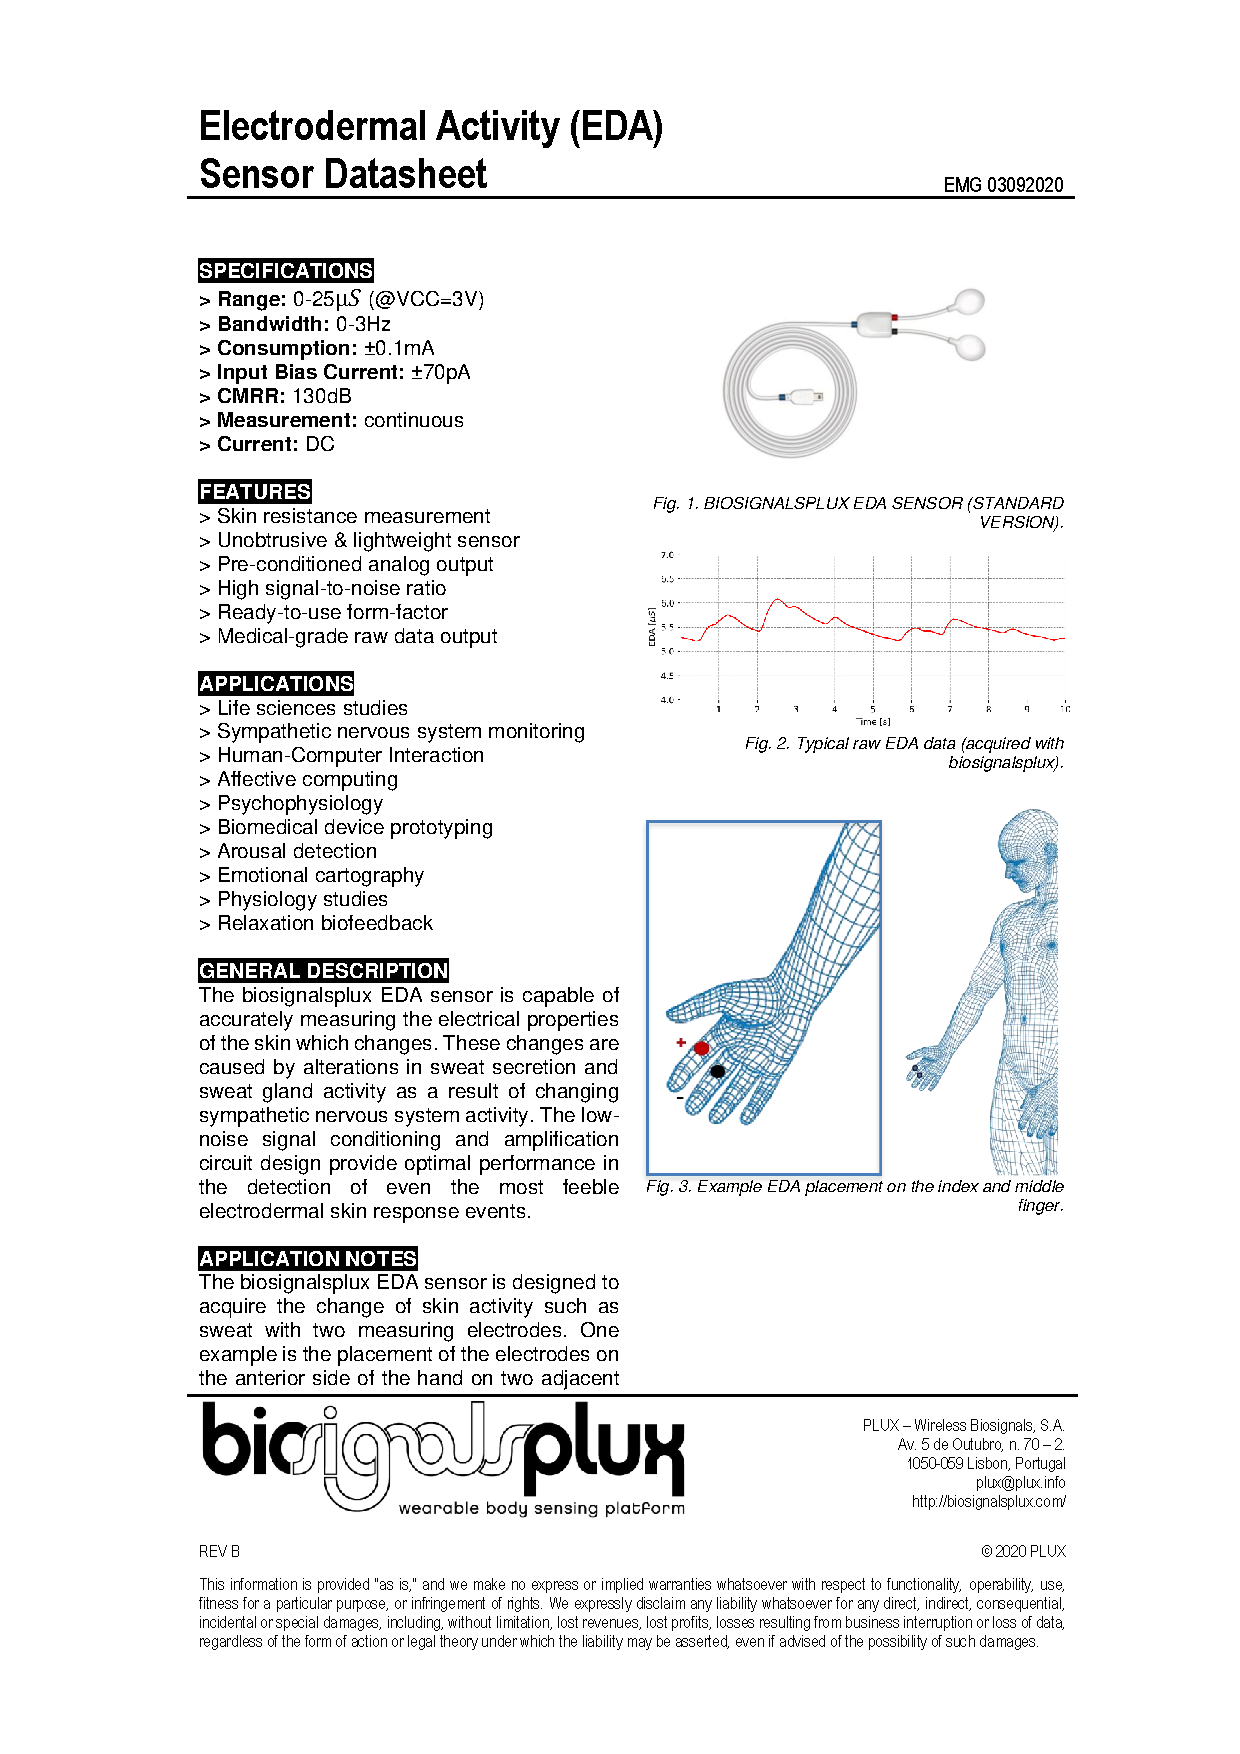
\includepdf[pages=-,width=\textwidth,pagecommand={}]{appendix/appendix-I.pdf}



\clearpage
\hypertarget{appendix-j-full-thematic-coding}{%
\subsection{Appendix L: Full Thematic Coding}\label{appendix-j-full-thematic-coding}}

This Appendix documents the complete coding underlying the reflexive thematic analysis reported in Chapter 5. It shows the full codebook, every coded data extract (not a selection), a code-frequency summary, and how the codes were consolidated into the five final themes. It is provided so the analysis can be inspected rather than taken on trust.

Sources are marked: {[}R{]} written post-task response, {[}Q{]} open-ended questionnaire item ("what made you feel that way"), {[}N{]} researcher observation note. Extracts are verbatim (participants\textquotesingle{} own spelling). N = 12, both conditions.

All participant extracts are reproduced verbatim from the typed written responses and observation notes; spelling and typing errors in the originals have been retained and are not individually marked.

\hypertarget{part-a.-codebook-30-codes}{%
\subsubsection{Part A. Codebook (30 codes)}\label{part-a.-codebook-30-codes}}

\Needspace{26\baselineskip}
\hypertarget{deductive-codes-defined-before-analysis}{%
\paragraph{Deductive codes (defined before analysis)}\label{deductive-codes-defined-before-analysis}}

\begin{longtable}[]{@{}
  >{\raggedright\arraybackslash}p{(\columnwidth - 4\tabcolsep) * \real{0.0525}}
  >{\raggedright\arraybackslash}p{(\columnwidth - 4\tabcolsep) * \real{0.3763}}
  >{\raggedright\arraybackslash}p{(\columnwidth - 4\tabcolsep) * \real{0.5513}}@{}}
\toprule\noalign{}
\begin{minipage}[t]{\linewidth}\raggedright
\textbf{ID}
\end{minipage} & \begin{minipage}[t]{\linewidth}\raggedright
\textbf{Code}
\end{minipage} & \begin{minipage}[t]{\linewidth}\raggedright
\textbf{Definition}
\end{minipage} \\
\begin{minipage}[t]{\linewidth}\raggedright
D1
\end{minipage} & \begin{minipage}[t]{\linewidth}\raggedright
Uncertainty about task state
\end{minipage} & \begin{minipage}[t]{\linewidth}\raggedright
Not knowing whether a step was done correctly or what to do next
\end{minipage} \\
\begin{minipage}[t]{\linewidth}\raggedright
D2
\end{minipage} & \begin{minipage}[t]{\linewidth}\raggedright
Needing help or external reference
\end{minipage} & \begin{minipage}[t]{\linewidth}\raggedright
Reliance on the experimenter, reference sheets, or manuals to proceed
\end{minipage} \\
\begin{minipage}[t]{\linewidth}\raggedright
D3
\end{minipage} & \begin{minipage}[t]{\linewidth}\raggedright
Sequence or step error
\end{minipage} & \begin{minipage}[t]{\linewidth}\raggedright
Doing steps out of order or in the wrong place
\end{minipage} \\
\begin{minipage}[t]{\linewidth}\raggedright
D4
\end{minipage} & \begin{minipage}[t]{\linewidth}\raggedright
Repeated calibration or baseline
\end{minipage} & \begin{minipage}[t]{\linewidth}\raggedright
Redoing a calibration or the EDA baseline
\end{minipage} \\
\begin{minipage}[t]{\linewidth}\raggedright
D5
\end{minipage} & \begin{minipage}[t]{\linewidth}\raggedright
Ease of use
\end{minipage} & \begin{minipage}[t]{\linewidth}\raggedright
Experiencing the workflow as easy, smooth, or intuitive
\end{minipage} \\
\begin{minipage}[t]{\linewidth}\raggedright
D6
\end{minipage} & \begin{minipage}[t]{\linewidth}\raggedright
Complexity or overwhelm
\end{minipage} & \begin{minipage}[t]{\linewidth}\raggedright
Experiencing the workflow as complex, cumbersome, or presenting too much at once
\end{minipage} \\
\begin{minipage}[t]{\linewidth}\raggedright
D7
\end{minipage} & \begin{minipage}[t]{\linewidth}\raggedright
Calibration confidence
\end{minipage} & \begin{minipage}[t]{\linewidth}\raggedright
Stated confidence, or its absence, that sensors were correctly calibrated
\end{minipage} \\
\begin{minipage}[t]{\linewidth}\raggedright
D8
\end{minipage} & \begin{minipage}[t]{\linewidth}\raggedright
Feedback and visibility of system status
\end{minipage} & \begin{minipage}[t]{\linewidth}\raggedright
Presence or absence of system feedback confirming state and progress
\end{minipage} \\
\begin{minipage}[t]{\linewidth}\raggedright
D9
\end{minipage} & \begin{minipage}[t]{\linewidth}\raggedright
First-time difficulty and learnability
\end{minipage} & \begin{minipage}[t]{\linewidth}\raggedright
Being hard on first encounter but expected to ease with familiarity
\end{minipage} \\
\begin{minipage}[t]{\linewidth}\raggedright
D10
\end{minipage} & \begin{minipage}[t]{\linewidth}\raggedright
Integration versus tool-switching
\end{minipage} & \begin{minipage}[t]{\linewidth}\raggedright
Everything in one place versus juggling separate tools
\end{minipage} \\
\begin{minipage}[t]{\linewidth}\raggedright
D11
\end{minipage} & \begin{minipage}[t]{\linewidth}\raggedright
Instructions at the point of need
\end{minipage} & \begin{minipage}[t]{\linewidth}\raggedright
Whether guidance was available where required, versus gaps
\end{minipage} \\
\begin{minipage}[t]{\linewidth}\raggedright
D12
\end{minipage} & \begin{minipage}[t]{\linewidth}\raggedright
Error prevention and recovery
\end{minipage} & \begin{minipage}[t]{\linewidth}\raggedright
The workflow catching or recovering from mistakes, versus letting them happen
\end{minipage} \\
\midrule\noalign{}
\endhead
\bottomrule\noalign{}
\endlastfoot
\end{longtable}

\phantomsection\addcontentsline{lot}{table}{\protect\numberline{L.1}Deductive codebook.}%
\textbf{Table L.1} Deductive codebook. The twelve codes and their definitions, derived before analysis from the interaction-breakdown categories, the usability constructs, and the Nielsen heuristics.

\Needspace{33\baselineskip}
\hypertarget{inductive-codes-developed-from-the-data}{%
\paragraph{Inductive codes (developed from the data)}\label{inductive-codes-developed-from-the-data}}

\begin{longtable}[]{@{}
  >{\raggedright\arraybackslash}p{(\columnwidth - 4\tabcolsep) * \real{0.0516}}
  >{\raggedright\arraybackslash}p{(\columnwidth - 4\tabcolsep) * \real{0.3868}}
  >{\raggedright\arraybackslash}p{(\columnwidth - 4\tabcolsep) * \real{0.5416}}@{}}
\toprule\noalign{}
\begin{minipage}[t]{\linewidth}\raggedright
\textbf{ID}
\end{minipage} & \begin{minipage}[t]{\linewidth}\raggedright
\textbf{Code}
\end{minipage} & \begin{minipage}[t]{\linewidth}\raggedright
\textbf{Definition}
\end{minipage} \\
\begin{minipage}[t]{\linewidth}\raggedright
I1
\end{minipage} & \begin{minipage}[t]{\linewidth}\raggedright
Jupyter and Python as a barrier
\end{minipage} & \begin{minipage}[t]{\linewidth}\raggedright
The fragmented EDA computation step in Jupyter as a distinct difficulty
\end{minipage} \\
\begin{minipage}[t]{\linewidth}\raggedright
I2
\end{minipage} & \begin{minipage}[t]{\linewidth}\raggedright
Record-versus-play confusion (OpenSignals)
\end{minipage} & \begin{minipage}[t]{\linewidth}\raggedright
Pressing play instead of record in the recording software
\end{minipage} \\
\begin{minipage}[t]{\linewidth}\raggedright
I3
\end{minipage} & \begin{minipage}[t]{\linewidth}\raggedright
Hardware connection uncertainty
\end{minipage} & \begin{minipage}[t]{\linewidth}\raggedright
Not being able to tell whether the hub or Bluetooth was connected
\end{minipage} \\
\begin{minipage}[t]{\linewidth}\raggedright
I4
\end{minipage} & \begin{minipage}[t]{\linewidth}\raggedright
Finding calibration in Tobii Core
\end{minipage} & \begin{minipage}[t]{\linewidth}\raggedright
Difficulty locating how to start calibration in the Tobii software
\end{minipage} \\
\begin{minipage}[t]{\linewidth}\raggedright
I5
\end{minipage} & \begin{minipage}[t]{\linewidth}\raggedright
Verification and validation reassurance
\end{minipage} & \begin{minipage}[t]{\linewidth}\raggedright
Confidence produced by an explicit calibration result or success confirmation
\end{minipage} \\
\begin{minipage}[t]{\linewidth}\raggedright
I6
\end{minipage} & \begin{minipage}[t]{\linewidth}\raggedright
Colour-coded and visual feedback valued
\end{minipage} & \begin{minipage}[t]{\linewidth}\raggedright
Positive response to green ticks, colour coding, progress bars, indicators
\end{minipage} \\
\begin{minipage}[t]{\linewidth}\raggedright
I7
\end{minipage} & \begin{minipage}[t]{\linewidth}\raggedright
Step-by-step guided flow valued
\end{minipage} & \begin{minipage}[t]{\linewidth}\raggedright
Appreciation of being led one step at a time
\end{minipage} \\
\begin{minipage}[t]{\linewidth}\raggedright
I8
\end{minipage} & \begin{minipage}[t]{\linewidth}\raggedright
Sensor recommendation valued
\end{minipage} & \begin{minipage}[t]{\linewidth}\raggedright
Positive response to the system recommending sensors and explaining why
\end{minipage} \\
\begin{minipage}[t]{\linewidth}\raggedright
I9
\end{minipage} & \begin{minipage}[t]{\linewidth}\raggedright
Metrics and feedback for non-experts
\end{minipage} & \begin{minipage}[t]{\linewidth}\raggedright
Value in the system surfacing signal quality to non-experts
\end{minipage} \\
\begin{minipage}[t]{\linewidth}\raggedright
I10
\end{minipage} & \begin{minipage}[t]{\linewidth}\raggedright
Electrode placement ambiguity
\end{minipage} & \begin{minipage}[t]{\linewidth}\raggedright
Uncertainty about hand or finger placement, tied to the placement illustration
\end{minipage} \\
\begin{minipage}[t]{\linewidth}\raggedright
I11
\end{minipage} & \begin{minipage}[t]{\linewidth}\raggedright
EDA value interpretation gap
\end{minipage} & \begin{minipage}[t]{\linewidth}\raggedright
Being shown an EDA value without knowing how to interpret it
\end{minipage} \\
\begin{minipage}[t]{\linewidth}\raggedright
I12
\end{minipage} & \begin{minipage}[t]{\linewidth}\raggedright
Reading and text burden
\end{minipage} & \begin{minipage}[t]{\linewidth}\raggedright
Too much text, and a preference for images or audio over reading
\end{minipage} \\
\begin{minipage}[t]{\linewidth}\raggedright
I13
\end{minipage} & \begin{minipage}[t]{\linewidth}\raggedright
Tool-switching burden
\end{minipage} & \begin{minipage}[t]{\linewidth}\raggedright
The labour of opening multiple applications, tabs, and downloads
\end{minipage} \\
\begin{minipage}[t]{\linewidth}\raggedright
I14
\end{minipage} & \begin{minipage}[t]{\linewidth}\raggedright
Prior-experience and order effect
\end{minipage} & \begin{minipage}[t]{\linewidth}\raggedright
The second condition feeling easier due to having done the first
\end{minipage} \\
\begin{minipage}[t]{\linewidth}\raggedright
I15
\end{minipage} & \begin{minipage}[t]{\linewidth}\raggedright
Eye-tracker positioning discomfort
\end{minipage} & \begin{minipage}[t]{\linewidth}\raggedright
Physical discomfort during positioning and distance adjustment
\end{minipage} \\
\begin{minipage}[t]{\linewidth}\raggedright
I16
\end{minipage} & \begin{minipage}[t]{\linewidth}\raggedright
Baseline and live-graph anxiety
\end{minipage} & \begin{minipage}[t]{\linewidth}\raggedright
The live graph or baseline value creating self-consciousness or doubt
\end{minipage} \\
\begin{minipage}[t]{\linewidth}\raggedright
I17
\end{minipage} & \begin{minipage}[t]{\linewidth}\raggedright
Account or profile setup friction
\end{minipage} & \begin{minipage}[t]{\linewidth}\raggedright
Confusion at the account, profile, or project-details setup stage
\end{minipage} \\
\begin{minipage}[t]{\linewidth}\raggedright
I18
\end{minipage} & \begin{minipage}[t]{\linewidth}\raggedright
Self-directed problem-solving
\end{minipage} & \begin{minipage}[t]{\linewidth}\raggedright
Working difficulties out alone, sometimes framed as mastery
\end{minipage} \\
\midrule\noalign{}
\endhead
\bottomrule\noalign{}
\endlastfoot
\end{longtable}

\phantomsection\addcontentsline{lot}{table}{\protect\numberline{L.2}Inductive codebook.}%
\textbf{Table L.2} Inductive codebook. The eighteen codes and their definitions, developed during analysis from the participants\textquotesingle{} written responses and the observation notes.

\hypertarget{part-b.-coded-data-extracts-all-instances}{%
\subsubsection{Part B. Coded data extracts (all instances)}\label{part-b.-coded-data-extracts-all-instances}}

\textbf{P01}

\textbf{Fragmented}

\begin{itemize}
\item
  "very confused at the beginning which made me go back to trying the process again" {[}R{]} -\textgreater{} D1, D4
\item
  "The process didnt feel confident and promising" {[}R{]} -\textgreater{} D7
\item
  "It was also strenuous for my eyes" {[}R{]} -\textgreater{} I15
\item
  "the calibration is very misleading and confusing" {[}R{]} -\textgreater{} D1, D6
\item
  "instructions could be a little more pictorial... a lot of extra information" {[}R{]} -\textgreater{} D11, I12
\item
  "not confident if i did it correct... needed help in confirming if the device is calibrated" {[}R{]} -\textgreater{} D1, D2, D8
\item
  "definitly not use it everyday as it is a lengthy process and very confusing" {[}R{]} -\textgreater{} D6
\item
  "rather listen to the instructions than reading them" {[}R{]} -\textgreater{} I12
\item
  "The python codes are very tiny and not understandable by every user" {[}R{]} -\textgreater{} I1
\item
  "a step wise guide would have been more helpfull" {[}R{]} -\textgreater{} D11, I7
\item
  "I didnt get a validation that I am correctly doing it" {[}Q{]} -\textgreater{} D8, I5
\item
  "slight struggle to find calibration screen" {[}N{]} -\textgreater{} I4
\item
  "not sure if bluetooth is connected for eda" {[}N{]} -\textgreater{} I3
\item
  "confused it with play button... clicked on play instead of record" {[}N{]} -\textgreater{} I2
\end{itemize}

\textbf{Unified}

\begin{itemize}
\item
  "It felt good and confident and easy as it was less of reading minute details" {[}R{]} -\textgreater{} D5, D7, I12
\item
  "very easy this time its just that i missed a step as i didnt read properly" {[}R{]} -\textgreater{} D5, D3
\item
  "the coloured responses with the icon was better to understand and a feel good factor" {[}R{]} -\textgreater{} D8, I6
\item
  "very promising this time to see the validation and the calibration is done correctly" {[}R{]} -\textgreater{} I5, D7
\item
  "easy instructions with the graphic... made me feel confident" {[}R{]} -\textgreater{} D11, I6, D7
\item
  "two buttons of the same colour and i thought i directly can jump to the calibration" {[}R{]} -\textgreater{} D1
\item
  "didnt really have to look at the instructions most of the time" {[}R{]} -\textgreater{} D5
\item
  "The green ticks and the progress bar assured me that i am on right track" {[}Q{]} -\textgreater{} D8, I6, I5
\item
  "liked that it recommended sensors" {[}N{]} -\textgreater{} I8
\item
  "likes the hub channel connectivity indicators" {[}N{]} -\textgreater{} D8, I6
\end{itemize}

\textbf{P02}

\textbf{Fragmented}

\begin{itemize}
\item
  "already knew what i am going to be doing" {[}R{]} -\textgreater{} I14
\item
  "instructions were clearer because of the support documents" {[}R{]} -\textgreater{} D11
\item
  "had to recalibrate the eye tracker again because i felt the values were off" {[}R{]} -\textgreater{} D4, D1
\item
  "could setup on my own and calibrate both devices on my own with no help" {[}R{]} -\textgreater{} I18
\item
  "couldnt find the tobi tracker software for a min but my instructor guided me" {[}R{]} -\textgreater{} I4, D2
\item
  "baseline value was right for the eda sensor, the eye tracker value was proper" {[}R{]} -\textgreater{} D7, D8
\item
  "open multiple tabs... two different softwares... download data from both... too much" {[}R{]} -\textgreater{} I13, D10
\item
  "software for the eda was in particular a little complex" {[}R{]} -\textgreater{} D6
\item
  "didnt know if the device had been connected and had to recheck" {[}R{]} -\textgreater{} I3
\item
  "the previous workflow had everything at one place which was way better" {[}R{]} -\textgreater{} D10
\item
  "not sure if biosignalsplux hub is connected or not" {[}N{]} -\textgreater{} I3
\end{itemize}

\textbf{Unified}

\begin{itemize}
\item
  "a little nervous during some parts... i had only ever used these once" {[}R{]} -\textgreater{} D9
\item
  "The setup was easy" {[}R{]} -\textgreater{} D5
\item
  "the system told me everything i had to do and how to do it" {[}R{]} -\textgreater{} D11, I7
\item
  "time crunch... mis-clicked... felt confused for a moment" {[}R{]} -\textgreater{} D1
\item
  "not being able to detect my eyes and i had to sit at a distance... made my eyes uncomfortable" {[}R{]} -\textgreater{} I15, D1
\item
  "once i saw that the calibration was done and it had recorded everything well, i felt confident" {[}R{]} -\textgreater{} I5, D7, D8
\item
  "unsure though whether we have to complete the study within a certain time frame" {[}R{]} -\textgreater{} D1
\item
  "properly calibrated because the system told me so. All the values were marked in positive" {[}R{]} -\textgreater{} D8, I5
\item
  "add some additional instructions for the eye tracker part" {[}R{]} -\textgreater{} D11
\item
  "the first time was a little bit overwhelming but it was pretty easy for me" {[}R{]} -\textgreater{} D9, D5
\item
  "after the system showed me values of calibration and assured that the data is collected... i felt it was completed well" {[}Q{]} -\textgreater{} I5, D8, D7
\item
  "study setup text is too small making it difficult to read" {[}N{]} -\textgreater{} I12
\item
  "didnt place electrodes on step 1 but instead on step 3" {[}N{]} -\textgreater{} D3
\end{itemize}

P03

\textbf{Fragmented}

\begin{itemize}
\item
  "some errors came up but it was still easy to handle" {[}R{]} -\textgreater{} D5, D12
\item
  "I was unsure what to do at some points" {[}R{]} -\textgreater{} D1
\item
  "The information was enough and clear" {[}R{]} -\textgreater{} D11
\item
  "the accuracy may not be that high but just sufficient" {[}R{]} -\textgreater{} D7
\item
  "EDA was also fluctuating a lot... I don\textquotesingle t have any idea of how sensitive the sensor was" {[}R{]} -\textgreater{} D1, I11
\item
  "did not sit 60 cm away from the screen during eye tracker calibration" {[}N{]} -\textgreater{} I15
\item
  "annoyed because he doesnt know if electrode placement is good or not" {[}N{]} -\textgreater{} I10, D8
\item
  "confused about whether biosignals hardware hub is conected via bluetooth" {[}N{]} -\textgreater{} I3
\item
  "put sensors on dominant hand instead of non dominant hand" {[}N{]} -\textgreater{} I10
\item
  "pressed play button instead of record button in opensignals... keeps pressing play" {[}N{]} -\textgreater{} I2
\item
  "confused during exeuction h5 computation python script in jupyter lab" {[}N{]} -\textgreater{} I1
\end{itemize}

\textbf{Unified}

\begin{itemize}
\item
  "I struggled in calibrating the EDA, I think the live graph was affecting how to breath" {[}R{]} -\textgreater{} I16, D1
\item
  "the only problem was the EDA" {[}R{]} -\textgreater{} I16
\item
  "Just remove the EDA live graph" {[}R{]} -\textgreater{} I16
\item
  "I struggled in calibrating the EDA sensor" {[}Q{]} -\textgreater{} I16
\item
  "i didnt choose these sensors! - oh it\textquotesingle s recommending them to me, i get it... likes the why these sensors card" {[}N{]} -\textgreater{} I8
\item
  "electrode placement instruction shows only right hand... switched electrodes from dominant to non dominant after reading" {[}N{]} -\textgreater{} I10, D3
\end{itemize}

P04

\textbf{Fragmented}

\begin{itemize}
\item
  "The eye-tracking calibration went smoothly... calibrate it pretty quickly" {[}R{]} -\textgreater{} D5
\item
  "When it came to the EDA calibration in Jupyter Lab, I had absolutely no idea what to do" {[}R{]} -\textgreater{} I1, D1
\item
  "overwhelmed by the information, the text... A lot of code and no experience with Jupyter" {[}R{]} -\textgreater{} I1, D6, I12
\item
  "instructions in Jupyter Lab without so much text... Everything was jumbled together" {[}R{]} -\textgreater{} D11, I12
\item
  "I get a graph with values, but I don\textquotesingle t know how to interpret them" {[}R{]} -\textgreater{} I11, D1
\item
  "A message saying CALIBRATION SUCCESS would be helpful at this point" {[}R{]} -\textgreater{} I5, D8
\item
  "I found Jupyter Lab very confusing for the task Calibrate EDA" {[}R{]} -\textgreater{} I1
\item
  "no instructions or guidelines on how to reach my goal step by step. I had to figure out for myself" {[}Q{]} -\textgreater{} D11, I18
\item
  "could not find out mean eda value without guidance" {[}N{]} -\textgreater{} I1, D2
\item
  "confused how to validate eye tracking in Tobii core, used gaze trace" {[}N{]} -\textgreater{} I4
\item
  "i think im connected... i see nothing, im not sure if its connected or not" {[}N{]} -\textgreater{} I3
\item
  "i dont know what to do.. I want to calibrate it again" {[}N{]} -\textgreater{} D4, D1
\end{itemize}

\textbf{Unified}

\begin{itemize}
\item
  "guided step by step through the calibration process. It was very easy" {[}R{]} -\textgreater{} D5, I7, D11
\item
  "the user interface for the calibration process guides the user step by step" {[}R{]} -\textgreater{} I7
\item
  "there was enough information for each intermediate step" {[}R{]} -\textgreater{} D11
\item
  "The green indicator: Calibration complete... easily focus my eyes directly on the dots" {[}R{]} -\textgreater{} D8, I6, I5
\item
  "The value is given in μS, but I don\textquotesingle t know what to make of it" {[}R{]} -\textgreater{} I11
\item
  "The calibration response (CALIBRATION DONE SUCCESSFULLY)" {[}Q{]} -\textgreater{} I5, D8
\item
  "liked the recommedned sensors" {[}N{]} -\textgreater{} I8
\item
  "tried moving around laptop to adjust positioing" {[}N{]} -\textgreater{} I15
\item
  "assumed electordes need to put on right hand since the instruction image shows a right hand" {[}N{]} -\textgreater{} I10
\end{itemize}


\textbf{P05}

\textbf{Fragmented}

\begin{itemize}
\item
  "I liked the tasks" {[}R{]} -\textgreater{} D5
\item
  "it was hard that I didn\textquotesingle t know anything about how to start with Jupiter" {[}R{]} -\textgreater{} I1
\item
  "the printed instructions also helped a lot" {[}R{]} -\textgreater{} D11
\item
  "I feel confident about the calibration" {[}R{]} -\textgreater{} D7
\item
  "visual feedback from Tobii\textquotesingle s software is extremely helpful" {[}Q{]} -\textgreater{} D8
\item
  "didn\textquotesingle t get any sign or negative feedback from open signals" {[}Q{]} -\textgreater{} D8
\item
  "found Jupiter Lab a little bit hard to get at the beginning" {[}Q{]} -\textgreater{} I1
\item
  "I love that the outcome was a visual graphic" {[}Q{]} -\textgreater{} I6, I9
\item
  "could not find out how to calibrate initially... validated eye tracking with gaze trace" {[}N{]} -\textgreater{} I4
\item
  "struggling to find if biosignals hub is connected to bluetooth" {[}N{]} -\textgreater{} I3
\item
  "struggles to locate the recording feature in opensignals" {[}N{]} -\textgreater{} I2
\end{itemize}

\textbf{Unified}

\begin{itemize}
\item
  "Everything was very intuitive, I just got confused with recalibrating the eye tracking" {[}R{]} -\textgreater{} D5, D4, D1
\item
  "Very easy in general" {[}R{]} -\textgreater{} D5
\item
  "the instructions were helpful" {[}R{]} -\textgreater{} D11
\item
  "The constant feedback helped me a lot to know that they were well calibrated" {[}Q{]} -\textgreater{} D8, I5
\item
  "likes the sensor recommendations" {[}N{]} -\textgreater{} I8
\item
  "skipped the calibration step and tried validating directly" {[}N{]} -\textgreater{} D3
\item
  "user turned off the biognals hub and was confused so researcher had to step in" {[}N{]} -\textgreater{} D12, D2, I3
\end{itemize}

\textbf{P06}

\textbf{Fragmented}

\begin{itemize}
\item
  "stuck while pairing the EDA with OpenSignals. Then I read it and was successful" {[}R{]} -\textgreater{} I3, D2, D12
\item
  "confused at first how does Open Signals work. Then I figured it out on my own" {[}R{]} -\textgreater{} I18, D1
\item
  "if the instructions were written step by step anybody can do it" {[}R{]} -\textgreater{} D11, I7
\item
  "more instructions using the OpenSignals software... at first it may feel a bit overwhelming" {[}R{]} -\textgreater{} D11, D6
\item
  "no doubt after... The last attempt was assuring that it\textquotesingle s working properly" {[}R{]} -\textgreater{} D7, D12
\item
  "figured it out on my own. So that\textquotesingle s when my confidence rose" {[}Q{]} -\textgreater{} I18
\item
  "the Calibration felt good because of the pop up dots... satisfied that the dot didn\textquotesingle t actually popped when I looked away" {[}Q{]} -\textgreater{} I5, D8, D7
\item
  "confused by opensignals ui, could not find record button" {[}N{]} -\textgreater{} I2
\item
  "cannot tell if biosignalsplux hub hardware is conected to bluetooth" {[}N{]} -\textgreater{} I3
\item
  "lost in the open signals ui, cannot figure out how to record" {[}N{]} -\textgreater{} I2
\end{itemize}

\textbf{Unified}

\begin{itemize}
\item
  "really liked the look until the dot pops out about the sensor calibration. That actually increased my confidence" {[}R{]} -\textgreater{} I5, D8, D7
\item
  "putting the electrodes on my own, I really was unsure... picture in the setup should have been more precise" {[}R{]} -\textgreater{} I10
\item
  "It was given perfectly when needed" {[}R{]} -\textgreater{} D11
\item
  "It was calibrating everything perfectly. I was really confident after two tasks" {[}R{]} -\textgreater{} D7, D8, I5
\item
  "change is the instruction about wearing the electrodes... should have been a clear picture" {[}R{]} -\textgreater{} I10
\item
  "worried about the last task when it was getting value more than the baseline... my confidence dropped" {[}Q{]} -\textgreater{} I16, I11, D7
\item
  "put electorodes on wrong fingers despite reading on screen instructions" {[}N{]} -\textgreater{} I10
\item
  "not sure if biosignalsplux hub hardware is connected" {[}N{]} -\textgreater{} I3
\end{itemize}

\textbf{P07}

\textbf{Fragmented}

\begin{itemize}
\item
  "tricky as a first time user... But once I got the hang of it, I found it super easy" {[}R{]} -\textgreater{} D9, I14, D5
\item
  "stuck while trying to figure out how Jupyter worked... executed its scripts in blocks" {[}R{]} -\textgreater{} I1, D1
\item
  "a couple of essential steps missing that I had to figure out myself" {[}R{]} -\textgreater{} D11, I18
\item
  "Very confident. The onscreen test was accurate" {[}R{]} -\textgreater{} D7, D8
\item
  "Everything worked well except Jupyter Lab... prefer more detailed instruction" {[}R{]} -\textgreater{} I1, D11
\item
  "tested it using the provided on-screen guide and it largely pointed specifically towards what I was looking at" {[}Q{]} -\textgreater{} D8, I5
\item
  "could not find out where to calibrate in tobii... frustrated... spent atleast 5 mins" {[}N{]} -\textgreater{} I4, D1
\item
  "clicked on play button instead of record in opensignals" {[}N{]} -\textgreater{} I2
\item
  "not a big fan of jupyter lab" {[}N{]} -\textgreater{} I1
\end{itemize}

\textbf{Unified}

\begin{itemize}
\item
  "It felt extremely intuitive to use" {[}R{]} -\textgreater{} D5
\item
  "because I had already gone through a similar process with the fragmented task, I had some idea of what to expect" {[}R{]} -\textgreater{} I14, D5
\item
  "10/10 confident" {[}R{]} -\textgreater{} D7
\item
  "the point where it listed the recommendations, I thought I was supposed to make selections" {[}R{]} -\textgreater{} I8, D1
\item
  "overall experience was smooth" {[}Q{]} -\textgreater{} D5
\item
  "looks easier on the eye... quick and easy, i feel better" {[}N{]} -\textgreater{} D5
\item
  "dominant hand instrcution phrasing is confusing for the user" {[}N{]} -\textgreater{} I10
\item
  "noticably less frustrated when comparted to fragmented workflow" {[}N{]} -\textgreater{} D5
\end{itemize}

\textbf{P08}

\textbf{Fragmented}

\begin{itemize}
\item
  "For EDA sensors there was not enough clarity on how to use OpenSignals" {[}R{]} -\textgreater{} D11, I2
\item
  "While navigating through jupyter notebook and opensignals" (difficulty) {[}R{]} -\textgreater{} I1, I2
\item
  "Visible change in readings and a definite output measurement" {[}R{]} -\textgreater{} D8
\item
  "Access to Jupyter notebook and its subsequent instructions seemed to deliver lack of information" {[}R{]} -\textgreater{} I1, D11
\item
  "The correct application of instructions" {[}Q{]} -\textgreater{} D11
\item
  "clicked on play button instead of record in opensignals" {[}N{]} -\textgreater{} I2
\item
  "recorded correctly then accidentally deleted the eda recording" {[}N{]} -\textgreater{} D12, D4
\end{itemize}

\textbf{Unified}

\begin{itemize}
\item
  "Setup was seemingly complicated at first, however upon reading the instructions stepwise, it paved the way" {[}R{]} -\textgreater{} D9, D11, D12
\item
  "certain instructions in the manual (on paper) seemed relatively unclear compared to the ones on Sensa" {[}R{]} -\textgreater{} D11
\item
  "instructions on the manual showed inconsistencies in the language compared to the instructions provided on Sensa" {[}R{]} -\textgreater{} D11
\item
  "reapplying the instructions and recalibrating with a better instructional knowledge... gave a better reading" {[}R{]} -\textgreater{} D4, D12
\item
  "the minor fluctuations... in the first calibration made me suspect that the initial findings were slightly inaccurate" {[}Q{]} -\textgreater{} I16, D7, I11
\item
  "put sensors on dominant hand initially, then changed after reading on screen instructions" {[}N{]} -\textgreater{} I10, D3
\item
  "repeated baseline becasue I moved my hands" {[}N{]} -\textgreater{} D4
\end{itemize}

\textbf{P09}

\textbf{Fragmented}

\begin{itemize}
\item
  "steps felt as if they assumed that the user would know how exactly to maneuver... discomfort... given the unfamiliarity" {[}R{]} -\textgreater{} D11, D9
\item
  "direction towards which part of the Tobii software suite governed visual profiles" (difficulty) {[}R{]} -\textgreater{} I4
\item
  "steps were definitely missing large gaps of information... simply gave the broad strokes" {[}R{]} -\textgreater{} D11
\item
  "100\% confident given that I kept the Gaze Trace feature on... As for the EDA... wasn\textquotesingle t confident of the quality of the data, only that something was being recorded" {[}R{]} -\textgreater{} D8, D7, I11
\item
  "forsake the need for a ipynb file and instead just run a python script" {[}R{]} -\textgreater{} I1
\item
  "perfectly confident about the eye tracker\textquotesingle s calibration, not so much so about the EDA" {[}Q{]} -\textgreater{} D7
\item
  "calibration steps are different thatn what im used to" {[}N{]} -\textgreater{} D9, I14
\item
  "annoyed at Tobii Core because cannot find how to recalibrate" {[}N{]} -\textgreater{} I4, D4
\item
  "dislikes the UI" {[}N{]} -\textgreater{} D1
\end{itemize}

\textbf{Unified}

\begin{itemize}
\item
  "Having feedback on the calibration data was very nice" {[}R{]} -\textgreater{} D8, I9
\item
  "It felt pretty usable. No notable difficulties" {[}R{]} -\textgreater{} D5
\item
  "The written notes were similarly undetailed, but the software picked up the slack" {[}R{]} -\textgreater{} D11, D8
\item
  "as close to perfectly confident as can be from the perspective of someone who doesn\textquotesingle t have any prior experience with the EDA" {[}R{]} -\textgreater{} D7, I9
\item
  "The guidance through Sensa and the unified feel was definitely much appreciated" {[}R{]} -\textgreater{} I7, D10
\item
  "Much better direction from the software itself in the form of quality feedback for sensor and calibration data" {[}Q{]} -\textgreater{} D8, I9, I5
\item
  "I love that it\textquotesingle s giving me metrics as a non professional" {[}N{]} -\textgreater{} I9, I6
\item
  "likes the green coding for positive metrics" {[}N{]} -\textgreater{} I6, D8
\item
  "really likes the live waveform and the color indicators for metrics" {[}N{]} -\textgreater{} I6, I9
\end{itemize}

\textbf{P10}

\textbf{Fragmented}

\begin{itemize}
\item
  "I felt overwhelmed, lost and frustated. Each software has a different workflow and UI" {[}R{]} -\textgreater{} D6, I13, D10
\item
  "difficult. Definitely need technical supports to finish the task, especially for the last task" {[}R{]} -\textgreater{} D2, D6, I1
\item
  "Too much information is presented at the same time. Had to look for the instructions back and fort" {[}R{]} -\textgreater{} I12, D11
\item
  "I didn\textquotesingle t really know what was going on. Not sure that I had the steps correct" {[}R{]} -\textgreater{} D1
\item
  "It\textquotesingle d be a pain to go through this every time, opening different softwares and applications" {[}R{]} -\textgreater{} I13, D10
\item
  "Too many steps, unnecessary text, no instructions available, the UI doesn\textquotesingle t have clear hierachy and feedbacks" {[}Q{]} -\textgreater{} I12, D11, D8, D6
\item
  "skipped eye tracker validation" {[}N{]} -\textgreater{} D3
\item
  "pressed play instead of record in opensignals" {[}N{]} -\textgreater{} I2
\item
  "jupyter is really hard for me... I dont know whats goig on while trying to run h5 computiatio" {[}N{]} -\textgreater{} I1
\end{itemize}

\textbf{Unified}

\begin{itemize}
\item
  "I like the live feedbacks on the screen" {[}R{]} -\textgreater{} D8, I6
\item
  "I didn\textquotesingle t like to read many texts... especially when there\textquotesingle s technical terms" {[}R{]} -\textgreater{} I12
\item
  "It doesn\textquotesingle t feel difficult to do. But it wasn\textquotesingle t neccessarily plesant" {[}R{]} -\textgreater{} D5
\item
  "It\textquotesingle s too much information at the same time actually" {[}R{]} -\textgreater{} I12, D6
\item
  "the 0.6 result in the red box... I doubted that I sticked the sensors wrong... there\textquotesingle s no way to check it" {[}R{]} -\textgreater{} I11, I10, I16
\item
  "For the first time, it can cost me some times and energy to get used to the system" {[}R{]} -\textgreater{} D9
\item
  "I\textquotesingle d like to have more images and less text" {[}R{]} -\textgreater{} I12
\item
  "live feedback on the screen to tell me that the devices are working... For the EDA... wasn\textquotesingle t sure... there\textquotesingle s no feedback for it" {[}Q{]} -\textgreater{} D8, I6, I10
\item
  "validation instrctions were too fast for me" {[}N{]} -\textgreater{} D11
\item
  "too much text is overwhelming... too much happening on baseline step on one screen" {[}N{]} -\textgreater{} I12, D6
\end{itemize}

\textbf{P11}

\textbf{Fragmented}

\begin{itemize}
\item
  "I found the task required many diiferet references to finish the entyire task" {[}R{]} -\textgreater{} I13, D2
\item
  "i had to refer to the reference papers multiple time" {[}R{]} -\textgreater{} D2, I13
\item
  "quite confident" {[}R{]} -\textgreater{} D7
\item
  "i would like a more streamlined workflow" {[}R{]} -\textgreater{} D10, D6
\item
  "thr color coded text" (source of confidence) {[}Q{]} -\textgreater{} I6, D8
\item
  "skipped the eye tracker validation step" {[}N{]} -\textgreater{} D3
\item
  "cannot tell if biosignals hub is connected" {[}N{]} -\textgreater{} I3
\item
  "pressed play button instead of record in opensignals" {[}N{]} -\textgreater{} I2
\end{itemize}

\textbf{Unified}

\begin{itemize}
\item
  "I found it little confusing while filling or setting up my user account" {[}R{]} -\textgreater{} I17
\item
  "Setup little confusing, not difficult. calibration easy and quick" {[}R{]} -\textgreater{} I17, D5
\item
  "pretty confident, because of the color-coded text being provided by the application" {[}R{]} -\textgreater{} I6, D8, D7
\item
  "a list of all the instruction task following the same sequence... would have made it more easier" {[}R{]} -\textgreater{} D11
\item
  "there were signals or texts in the application that instructed whether the task was completed or not" {[}Q{]} -\textgreater{} D8, I5
\item
  "no feedback from hub hardware is confusing" {[}N{]} -\textgreater{} I3, D8
\item
  "do i peel off the electrode sickers?" {[}N{]} -\textgreater{} I10, D1
\item
  "brought laptop closer instead of moving chair back in eye tracker positioning step" {[}N{]} -\textgreater{} I15
\end{itemize}

\textbf{P12}

\textbf{Fragmented}

\begin{itemize}
\item
  "a little confused and hesitant... but with the instruction manuals... it became easier to go with the flow" {[}R{]} -\textgreater{} D1, D11, D12
\item
  "couldn\textquotesingle t understand and find the button to click to find the option to create the profile" {[}R{]} -\textgreater{} I17
\item
  "when i calibrated first time i wasnt quiet sure if i did it correctly or not" {[}R{]} -\textgreater{} D1, D7
\item
  "prefer a little more detailed description for onboarding" {[}R{]} -\textgreater{} D11
\item
  "confused with the eye tracking calibration in start as the interface of tobi core felt confusing" {[}R{]} -\textgreater{} I4, D1
\item
  "after i calibrated the data for the second time i felt a bit more confident and the pop message... calibration done sucessfully" {[}Q{]} -\textgreater{} D4, I5, D7
\item
  "couldn\textquotesingle t find out how to calibrate eyetracker spending a lot of time on it" {[}N{]} -\textgreater{} I4
\item
  "i feel like i did the eye tracker validation via tobii core correct i dont know" {[}N{]} -\textgreater{} D1
\item
  "connected the hub but disabled the bluetooth in opensignals causing confusion" {[}N{]} -\textgreater{} I3
\end{itemize}

\textbf{Unified}

\begin{itemize}
\item
  "quiet confident and felt the interface quiet engaging... the interface felt like a helping guide instead of overwhelming" {[}R{]} -\textgreater{} D5, I7, D8
\item
  "easy and quiet simple to setup, I just got stuck once when the system was checking signals for the EDA" {[}R{]} -\textgreater{} D5, D1
\item
  "it was like a step by step guide and took me through the journey with one step at a time instead of overwhelming me" {[}R{]} -\textgreater{} I7, D11
\item
  "especially the task completion message the popped at end made it feel more confident" {[}R{]} -\textgreater{} I5, D8, D7
\item
  "I might play around with the positioning of text and font and layout in the biosignals recording screen" {[}R{]} -\textgreater{} I12
\item
  "well oraganised, not overwhelming... provided all necessary information needed to proceed with the step at each time" {[}Q{]} -\textgreater{} I7, D11
\item
  "i could see all required information at a single screen instead of different place" {[}Q{]} -\textgreater{} D10
\item
  "liked the idea timer on the screen way better compared to the fragmented" {[}Q{]} -\textgreater{} D8, I6
\item
  "likes the on screen timer in the baseline recording" {[}N{]} -\textgreater{} D8, I6
\end{itemize}

\Needspace{40\baselineskip}
\hypertarget{part-c.-code-application-summary}{%
\subsubsection{Part C. Code application summary}\label{part-c.-code-application-summary}}

Participants in whom each code appeared, by condition (F = fragmented, U = unified).

\begingroup\let\small\footnotesize\setlength{\tabcolsep}{4pt}
\begin{longtable}[]{@{}
  >{\raggedright\arraybackslash}p{(\columnwidth - 4\tabcolsep) * \real{0.2809}}
  >{\raggedright\arraybackslash}p{(\columnwidth - 4\tabcolsep) * \real{0.3659}}
  >{\raggedright\arraybackslash}p{(\columnwidth - 4\tabcolsep) * \real{0.3332}}@{}}
\toprule\noalign{}
\begin{minipage}[t]{\linewidth}\raggedright
\textbf{Code}
\end{minipage} & \begin{minipage}[t]{\linewidth}\raggedright
\textbf{Fragmented}
\end{minipage} & \begin{minipage}[t]{\linewidth}\raggedright
\textbf{Unified}
\end{minipage} \\
\begin{minipage}[t]{\linewidth}\raggedright
\textbf{D1} Uncertainty about task state
\end{minipage} & \begin{minipage}[t]{\linewidth}\raggedright
P01, P02, P03, P04, P06, P07, P09, P10, P12
\end{minipage} & \begin{minipage}[t]{\linewidth}\raggedright
P01, P02, P03, P05, P07, P11, P12
\end{minipage} \\
\begin{minipage}[t]{\linewidth}\raggedright
\textbf{D2} Needing help / external reference
\end{minipage} & \begin{minipage}[t]{\linewidth}\raggedright
P01, P02, P04, P06, P10, P11
\end{minipage} & \begin{minipage}[t]{\linewidth}\raggedright
P05
\end{minipage} \\
\begin{minipage}[t]{\linewidth}\raggedright
\textbf{D3} Sequence or step error
\end{minipage} & \begin{minipage}[t]{\linewidth}\raggedright
P10, P11
\end{minipage} & \begin{minipage}[t]{\linewidth}\raggedright
P01, P02, P03, P05, P08
\end{minipage} \\
\begin{minipage}[t]{\linewidth}\raggedright
\textbf{D4} Repeated calibration or baseline
\end{minipage} & \begin{minipage}[t]{\linewidth}\raggedright
P01, P02, P04, P08, P09, P12
\end{minipage} & \begin{minipage}[t]{\linewidth}\raggedright
P05, P08
\end{minipage} \\
\begin{minipage}[t]{\linewidth}\raggedright
\textbf{D5} Ease of use
\end{minipage} & \begin{minipage}[t]{\linewidth}\raggedright
P03, P04, P05, P07
\end{minipage} & \begin{minipage}[t]{\linewidth}\raggedright
P01, P02, P04, P05, P07, P09, P10, P11, P12
\end{minipage} \\
\begin{minipage}[t]{\linewidth}\raggedright
\textbf{D6} Complexity or overwhelm
\end{minipage} & \begin{minipage}[t]{\linewidth}\raggedright
P01, P02, P04, P06, P10, P11
\end{minipage} & \begin{minipage}[t]{\linewidth}\raggedright
P10
\end{minipage} \\
\begin{minipage}[t]{\linewidth}\raggedright
\textbf{D7} Calibration confidence
\end{minipage} & \begin{minipage}[t]{\linewidth}\raggedright
P01, P02, P03, P05, P06, P07, P09, P11, P12
\end{minipage} & \begin{minipage}[t]{\linewidth}\raggedright
P01, P02, P06, P07, P08, P09, P11, P12
\end{minipage} \\
\begin{minipage}[t]{\linewidth}\raggedright
\textbf{D8} Feedback / visibility of status
\end{minipage} & \begin{minipage}[t]{\linewidth}\raggedright
P01, P02, P03, P04, P05, P06, P07, P08, P09, P10, P11
\end{minipage} & \begin{minipage}[t]{\linewidth}\raggedright
P01, P02, P04, P05, P06, P09, P10, P11, P12
\end{minipage} \\
\begin{minipage}[t]{\linewidth}\raggedright
\textbf{D9} First-time difficulty / learnability
\end{minipage} & \begin{minipage}[t]{\linewidth}\raggedright
P07, P09
\end{minipage} & \begin{minipage}[t]{\linewidth}\raggedright
P02, P08, P10
\end{minipage} \\
\begin{minipage}[t]{\linewidth}\raggedright
\textbf{D10} Integration vs tool-switching
\end{minipage} & \begin{minipage}[t]{\linewidth}\raggedright
P02, P10, P11
\end{minipage} & \begin{minipage}[t]{\linewidth}\raggedright
P09, P12
\end{minipage} \\
\begin{minipage}[t]{\linewidth}\raggedright
\textbf{D11} Instructions at point of need
\end{minipage} & \begin{minipage}[t]{\linewidth}\raggedright
P01, P02, P03, P04, P05, P06, P07, P08, P09, P10, P12
\end{minipage} & \begin{minipage}[t]{\linewidth}\raggedright
P01, P02, P04, P05, P06, P08, P09, P10, P11, P12
\end{minipage} \\
\begin{minipage}[t]{\linewidth}\raggedright
\textbf{D12} Error prevention and recovery
\end{minipage} & \begin{minipage}[t]{\linewidth}\raggedright
P03, P06, P08, P12
\end{minipage} & \begin{minipage}[t]{\linewidth}\raggedright
P05, P08
\end{minipage} \\
\begin{minipage}[t]{\linewidth}\raggedright
\textbf{I1} Jupyter / Python barrier
\end{minipage} & \begin{minipage}[t]{\linewidth}\raggedright
P01, P03, P04, P05, P07, P08, P09, P10
\end{minipage} & \begin{minipage}[t]{\linewidth}\raggedright
-
\end{minipage} \\
\begin{minipage}[t]{\linewidth}\raggedright
\textbf{I2} Record-versus-play confusion
\end{minipage} & \begin{minipage}[t]{\linewidth}\raggedright
P01, P03, P05, P06, P07, P08, P10, P11
\end{minipage} & \begin{minipage}[t]{\linewidth}\raggedright
-
\end{minipage} \\
\begin{minipage}[t]{\linewidth}\raggedright
\textbf{I3} Hardware connection uncertainty
\end{minipage} & \begin{minipage}[t]{\linewidth}\raggedright
P01, P02, P03, P04, P05, P06, P11, P12
\end{minipage} & \begin{minipage}[t]{\linewidth}\raggedright
P05, P06, P11
\end{minipage} \\
\begin{minipage}[t]{\linewidth}\raggedright
\textbf{I4} Finding calibration in Tobii Core
\end{minipage} & \begin{minipage}[t]{\linewidth}\raggedright
P01, P02, P04, P05, P07, P09, P12
\end{minipage} & \begin{minipage}[t]{\linewidth}\raggedright
-
\end{minipage} \\
\begin{minipage}[t]{\linewidth}\raggedright
\textbf{I5} Verification / validation reassurance
\end{minipage} & \begin{minipage}[t]{\linewidth}\raggedright
P01, P04, P06, P07, P12
\end{minipage} & \begin{minipage}[t]{\linewidth}\raggedright
P01, P02, P04, P05, P06, P09, P11, P12
\end{minipage} \\
\begin{minipage}[t]{\linewidth}\raggedright
\textbf{I6} Colour-coded / visual feedback valued
\end{minipage} & \begin{minipage}[t]{\linewidth}\raggedright
P05, P11
\end{minipage} & \begin{minipage}[t]{\linewidth}\raggedright
P01, P04, P09, P10, P11, P12
\end{minipage} \\
\begin{minipage}[t]{\linewidth}\raggedright
\textbf{I7} Step-by-step guided flow valued
\end{minipage} & \begin{minipage}[t]{\linewidth}\raggedright
P01, P06
\end{minipage} & \begin{minipage}[t]{\linewidth}\raggedright
P02, P04, P09, P12
\end{minipage} \\
\begin{minipage}[t]{\linewidth}\raggedright
\textbf{I8} Sensor recommendation valued
\end{minipage} & \begin{minipage}[t]{\linewidth}\raggedright
-
\end{minipage} & \begin{minipage}[t]{\linewidth}\raggedright
P01, P03, P04, P05, P07
\end{minipage} \\
\begin{minipage}[t]{\linewidth}\raggedright
\textbf{I9} Metrics / feedback for non-experts
\end{minipage} & \begin{minipage}[t]{\linewidth}\raggedright
P05
\end{minipage} & \begin{minipage}[t]{\linewidth}\raggedright
P09
\end{minipage} \\
\begin{minipage}[t]{\linewidth}\raggedright
\textbf{I10} Electrode placement ambiguity
\end{minipage} & \begin{minipage}[t]{\linewidth}\raggedright
P03
\end{minipage} & \begin{minipage}[t]{\linewidth}\raggedright
P03, P04, P06, P07, P08, P10, P11
\end{minipage} \\
\begin{minipage}[t]{\linewidth}\raggedright
\textbf{I11} EDA value interpretation gap
\end{minipage} & \begin{minipage}[t]{\linewidth}\raggedright
P03, P04, P09
\end{minipage} & \begin{minipage}[t]{\linewidth}\raggedright
P04, P06, P08, P10
\end{minipage} \\
\begin{minipage}[t]{\linewidth}\raggedright
\textbf{I12} Reading / text burden
\end{minipage} & \begin{minipage}[t]{\linewidth}\raggedright
P01, P04, P10
\end{minipage} & \begin{minipage}[t]{\linewidth}\raggedright
P01, P02, P10, P12
\end{minipage} \\
\begin{minipage}[t]{\linewidth}\raggedright
\textbf{I13} Tool-switching burden
\end{minipage} & \begin{minipage}[t]{\linewidth}\raggedright
P02, P10, P11
\end{minipage} & \begin{minipage}[t]{\linewidth}\raggedright
-
\end{minipage} \\
\begin{minipage}[t]{\linewidth}\raggedright
\textbf{I14} Prior-experience / order effect
\end{minipage} & \begin{minipage}[t]{\linewidth}\raggedright
P02, P07, P09
\end{minipage} & \begin{minipage}[t]{\linewidth}\raggedright
P07
\end{minipage} \\
\begin{minipage}[t]{\linewidth}\raggedright
\textbf{I15} Eye-tracker positioning discomfort
\end{minipage} & \begin{minipage}[t]{\linewidth}\raggedright
P01, P03
\end{minipage} & \begin{minipage}[t]{\linewidth}\raggedright
P02, P04, P11
\end{minipage} \\
\begin{minipage}[t]{\linewidth}\raggedright
\textbf{I16} Baseline / live-graph anxiety
\end{minipage} & \begin{minipage}[t]{\linewidth}\raggedright
-
\end{minipage} & \begin{minipage}[t]{\linewidth}\raggedright
P03, P06, P08, P10
\end{minipage} \\
\begin{minipage}[t]{\linewidth}\raggedright
\textbf{I17} Account / profile setup friction
\end{minipage} & \begin{minipage}[t]{\linewidth}\raggedright
P12
\end{minipage} & \begin{minipage}[t]{\linewidth}\raggedright
P11
\end{minipage} \\
\begin{minipage}[t]{\linewidth}\raggedright
\textbf{I18} Self-directed problem-solving
\end{minipage} & \begin{minipage}[t]{\linewidth}\raggedright
P02, P04, P06, P07
\end{minipage} & \begin{minipage}[t]{\linewidth}\raggedright
-
\end{minipage} \\
\midrule\noalign{}
\endhead
\bottomrule\noalign{}
\endlastfoot
\end{longtable}
\endgroup

\phantomsection\addcontentsline{lot}{table}{\protect\numberline{L.3}Code application by participant.}%
\textbf{Table L.3} Code application by participant. The participants in whom each of the thirty codes appeared, split by condition.

The pattern is directional and consistent with the quantitative results: the fragmented-heavy codes cluster around disconnected tools and hidden state (I1, I2, I3, I4, I13, D2, D6), while the unified-heavy codes cluster around visible feedback and guidance (I5, I6, I7, I8, D5, D8). Several codes are genuinely cross-cutting (I10, I11, I15, I16), and these are the residual problems that the unified workflow did not resolve.

\Needspace{16\baselineskip}
\hypertarget{part-d.-consolidation-into-the-five-themes}{%
\subsubsection{Part D. Consolidation into the five themes}\label{part-d.-consolidation-into-the-five-themes}}

\begingroup\renewcommand{\longtablestretch}{1.6}
\begin{longtable}[]{@{}
  >{\raggedright\arraybackslash}p{(\columnwidth - 4\tabcolsep) * \real{0.3358}}
  >{\raggedright\arraybackslash}p{(\columnwidth - 4\tabcolsep) * \real{0.2124}}
  >{\raggedright\arraybackslash}p{(\columnwidth - 4\tabcolsep) * \real{0.4317}}@{}}
\toprule\noalign{}
\begin{minipage}[t]{\linewidth}\raggedright
\textbf{Theme}
\end{minipage} & \begin{minipage}[t]{\linewidth}\raggedright
\textbf{Constituent codes}
\end{minipage} & \begin{minipage}[t]{\linewidth}\raggedright
\textbf{Rationale}
\end{minipage} \\
\begin{minipage}[t]{\linewidth}\raggedright
1. Confidence grounded in system feedback
\end{minipage} & \begin{minipage}[t]{\linewidth}\raggedright
D8, D7, D1, I5, I6, I9, I3
\end{minipage} & \begin{minipage}[t]{\linewidth}\raggedright
Confidence tracked with whether the system made its state visible; the absence of feedback (D8, I3, D1) produced uncertainty, and explicit confirmation (I5, I6, I9) produced confidence (D7). Includes the counter-cases where visible signals lowered confidence.
\end{minipage} \\
\begin{minipage}[t]{\linewidth}\raggedright
2. The burden of coordinating fragmented tools
\end{minipage} & \begin{minipage}[t]{\linewidth}\raggedright
I13, I1, I2, I4, D10, D6, D2
\end{minipage} & \begin{minipage}[t]{\linewidth}\raggedright
Fragmentation\textquotesingle s overhead: the labour of moving between disconnected tools (I13, D10), each with its own failure modes (I1 Jupyter, I2 record-vs-play, I4 finding calibration), producing overwhelm (D6) and reliance on help (D2).
\end{minipage} \\
\begin{minipage}[t]{\linewidth}\raggedright
3. Guidance from the system
\end{minipage} & \begin{minipage}[t]{\linewidth}\raggedright
D5, I7, I8, D11, D9
\end{minipage} & \begin{minipage}[t]{\linewidth}\raggedright
The unified workflow\textquotesingle s guidance lowered the barrier: step-by-step flow (I7), sensor recommendation (I8), and instructions at the point of need (D11) made it easy (D5), especially past first-time difficulty (D9).
\end{minipage} \\
\begin{minipage}[t]{\linewidth}\raggedright
4. The limits of guidance
\end{minipage} & \begin{minipage}[t]{\linewidth}\raggedright
I10, I11, I12, I16, I15, I17
\end{minipage} & \begin{minipage}[t]{\linewidth}\raggedright
The residual friction the guided flow did not remove: placement ambiguity from a shared illustration (I10), uninterpretable values (I11), text overload (I12), live-feedback anxiety (I16), positioning discomfort (I15).
\end{minipage} \\
\begin{minipage}[t]{\linewidth}\raggedright
5. Familiarity and order effects
\end{minipage} & \begin{minipage}[t]{\linewidth}\raggedright
I14, I18
\end{minipage} & \begin{minipage}[t]{\linewidth}\raggedright
Familiarity and self-reliance: ease partly from having done the other condition (I14) or from working it out alone (I18). Interpretive theme cautioning against attributing all ease to the workflow.
\end{minipage} \\
\midrule\noalign{}
\endhead
\bottomrule\noalign{}
\endlastfoot
\end{longtable}
\endgroup

\phantomsection\addcontentsline{lot}{table}{\protect\numberline{L.4}Consolidation into themes.}%
\textbf{Table L.4} Consolidation into themes. The codes constituting each of the final five themes, with the rationale for grouping.

Codes D3 (sequence errors) and D4 (repeated calibration and baseline) are procedural codes that correspond directly to breakdown categories counted under H4 (incorrect sequence execution, and repeated calibration and baseline recording; Table 5.3), so their quantitative side is reported there rather than as a separate theme. D12 (error recovery) is a cross-cutting recovery code that contextualises those breakdowns qualitatively (Chapter 6.4) rather than forming a count of its own. All three cut across Themes 1, 2, and 4 rather than sitting under one.

\clearpage
\hypertarget{appendix-k-per-participant-quantitative-data}{%
\subsection{Appendix M: Per-Participant Quantitative Data}\label{appendix-k-per-participant-quantitative-data}}

This appendix reports the complete per-participant dataset underlying the quantitative results in Chapter 5. Each participant completed both conditions, so every row contains a matched pair of values. F denotes the fragmented condition and U the unified condition.

Gaze accuracy and gaze precision are reported in degrees of visual angle. Interaction breakdown counts are totals across the five recorded categories, the per-category decomposition of which is given in Table 5.3. First-pass calibration success is recorded as pass or fail. Tables M.1 to M.4 report this dataset grouped by measure type: M.1 covers setup and calibration efficiency together with interaction breakdown counts; M.2 covers the subjective measures (NASA-TLX, SUS, and calibration confidence); M.3 covers eye-tracking calibration quality; and M.4 covers the EDA baseline.

\Needspace{24\baselineskip}
\begingroup\let\small\footnotesize\setlength{\tabcolsep}{4pt}
\Needspace{4\baselineskip}
\begingroup\let\small\footnotesize\setlength{\tabcolsep}{4pt}
\begin{longtable}[]{@{}>{\raggedright\arraybackslash}p{(\columnwidth - 14\tabcolsep) * \real{0.1100}}>{\raggedright\arraybackslash}p{(\columnwidth - 14\tabcolsep) * \real{0.1483}}>{\raggedright\arraybackslash}p{(\columnwidth - 14\tabcolsep) * \real{0.1483}}>{\raggedright\arraybackslash}p{(\columnwidth - 14\tabcolsep) * \real{0.1483}}>{\raggedright\arraybackslash}p{(\columnwidth - 14\tabcolsep) * \real{0.1483}}>{\raggedright\arraybackslash}p{(\columnwidth - 14\tabcolsep) * \real{0.1483}}>{\raggedright\arraybackslash}p{(\columnwidth - 14\tabcolsep) * \real{0.1483}}@{}}
\toprule\noalign{}
\textbf{Participant} & \textbf{Setup time (s) F} & \textbf{Setup time (s) U} & \textbf{Calibration time (s) F} & \textbf{Calibration time (s) U} & \textbf{Breakdowns F} & \textbf{Breakdowns U} \\
\midrule\noalign{}
\endhead
\bottomrule\noalign{}
\endlastfoot
P01 & 1645 & 837 & 1317 & 439 & 21 & 4 \\
P02 & 1263 & 1214 & 952 & 754 & 13 & 11 \\
P03 & 1571 & 1149 & 1236 & 775 & 24 & 8 \\
P04 & 1376 & 817 & 1071 & 502 & 16 & 2 \\
P05 & 1004 & 1001 & 614 & 774 & 12 & 8 \\
P06 & 1324 & 1062 & 1126 & 714 & 17 & 9 \\
P07 & 1412 & 1014 & 984 & 748 & 19 & 11 \\
P08 & 926 & 1170 & 646 & 798 & 22 & 13 \\
P09 & 1501 & 845 & 1121 & 571 & 23 & 2 \\
P10 & 779 & 1017 & 533 & 478 & 25 & 13 \\
P11 & 865 & 1256 & 666 & 1039 & 22 & 12 \\
P12 & 1040 & 599 & 845 & 407 & 26 & 5 \\
\textbf{Mean} & \textbf{1225.50} & \textbf{998.42} & \textbf{925.92} & \textbf{666.58} & \textbf{20.00} & \textbf{8.17} \\
\textbf{SD} & \textbf{292.68} & \textbf{193.44} & \textbf{262.23} & \textbf{187.51} & \textbf{4.61} & \textbf{4.06} \\
\end{longtable}
\endgroup
\endgroup

\phantomsection\addcontentsline{lot}{table}{\protect\numberline{M.1}Per-participant efficiency and interaction breakdowns.}%
\textbf{Table M.1} Per-participant efficiency and interaction breakdowns. Setup time, calibration time, and interaction breakdown counts for each participant (N = 12) in both conditions.

\Needspace{24\baselineskip}
\begingroup\let\small\footnotesize\setlength{\tabcolsep}{4pt}
\Needspace{4\baselineskip}
\begingroup\let\small\footnotesize\setlength{\tabcolsep}{4pt}
\begin{longtable}[]{@{}>{\raggedright\arraybackslash}p{(\columnwidth - 14\tabcolsep) * \real{0.1100}}>{\raggedright\arraybackslash}p{(\columnwidth - 14\tabcolsep) * \real{0.1483}}>{\raggedright\arraybackslash}p{(\columnwidth - 14\tabcolsep) * \real{0.1483}}>{\raggedright\arraybackslash}p{(\columnwidth - 14\tabcolsep) * \real{0.1483}}>{\raggedright\arraybackslash}p{(\columnwidth - 14\tabcolsep) * \real{0.1483}}>{\raggedright\arraybackslash}p{(\columnwidth - 14\tabcolsep) * \real{0.1483}}>{\raggedright\arraybackslash}p{(\columnwidth - 14\tabcolsep) * \real{0.1483}}@{}}
\toprule\noalign{}
\textbf{Participant} & \textbf{NASA-TLX F} & \textbf{NASA-TLX U} & \textbf{SUS F} & \textbf{SUS U} & \textbf{Confidence (1-7) F} & \textbf{Confidence (1-7) U} \\
\midrule\noalign{}
\endhead
\bottomrule\noalign{}
\endlastfoot
P01 & 71.67 & 11.67 & 12.5 & 87.5 & 3 & 7 \\
P02 & 15.00 & 41.67 & 90 & 65 & 7 & 6 \\
P03 & 35.00 & 10.00 & 50 & 82.5 & 6 & 2 \\
P04 & 65.00 & 6.67 & 10 & 82.5 & 2 & 7 \\
P05 & 43.33 & 8.33 & 87.5 & 90 & 7 & 7 \\
P06 & 40.00 & 28.33 & 72.5 & 72.5 & 6 & 5 \\
P07 & 13.33 & 0.00 & 62.5 & 100 & 6 & 7 \\
P08 & 45.00 & 40.00 & 30 & 55 & 7 & 5 \\
P09 & 28.33 & 20.00 & 57.5 & 85 & 5 & 6 \\
P10 & 73.33 & 61.67 & 0 & 42.5 & 1 & 6 \\
P11 & 56.67 & 33.33 & 27.5 & 32.5 & 6 & 5 \\
P12 & 36.67 & 5.00 & 57.5 & 85 & 5 & 6 \\
\textbf{Mean} & \textbf{43.61} & \textbf{22.22} & \textbf{46.46} & \textbf{73.33} & \textbf{5.08} & \textbf{5.75} \\
\textbf{SD} & \textbf{20.01} & \textbf{18.83} & \textbf{30.22} & \textbf{20.57} & \textbf{2.02} & \textbf{1.42} \\
\end{longtable}
\endgroup
\endgroup

\phantomsection\addcontentsline{lot}{table}{\protect\numberline{M.2}Per-participant subjective measures.}%
\textbf{Table M.2} Per-participant subjective measures. Raw NASA-TLX, System Usability Scale, and calibration confidence for each participant (N = 12) in both conditions.

\Needspace{24\baselineskip}
\begin{landscape}
\begingroup\let\small\footnotesize\setlength{\tabcolsep}{4pt}
\begingroup\let\small\footnotesize\setlength{\tabcolsep}{4pt}
\begin{longtable}[]{@{}>{\raggedright\arraybackslash}p{(\columnwidth - 18\tabcolsep) * \real{0.0650}}>{\raggedright\arraybackslash}p{(\columnwidth - 18\tabcolsep) * \real{0.1169}}>{\raggedright\arraybackslash}p{(\columnwidth - 18\tabcolsep) * \real{0.1169}}>{\raggedright\arraybackslash}p{(\columnwidth - 18\tabcolsep) * \real{0.1169}}>{\raggedright\arraybackslash}p{(\columnwidth - 18\tabcolsep) * \real{0.1169}}>{\raggedright\arraybackslash}p{(\columnwidth - 18\tabcolsep) * \real{0.1169}}>{\raggedright\arraybackslash}p{(\columnwidth - 18\tabcolsep) * \real{0.1169}}>{\raggedright\arraybackslash}p{(\columnwidth - 18\tabcolsep) * \real{0.1169}}>{\raggedright\arraybackslash}p{(\columnwidth - 18\tabcolsep) * \real{0.1169}}@{}}
\toprule\noalign{}
\textbf{Participant} & \textbf{Gaze accuracy (deg) F} & \textbf{Gaze accuracy (deg) U} & \textbf{Gaze precision (deg) F} & \textbf{Gaze precision (deg) U} & \textbf{Valid data yield (\%) F} & \textbf{Valid data yield (\%) U} & \textbf{First-pass F} & \textbf{First-pass U} \\
\midrule\noalign{}
\endhead
\bottomrule\noalign{}
\endlastfoot
P01 & 9.07 & 0.93 & 0.47 & 0.33 & 100.0 & 100.0 & Fail & Pass \\
P02 & 1.66 & 2.12 & 0.58 & 0.34 & 100.0 & 100.0 & Fail & Pass \\
P03 & 1.13 & 0.88 & 0.19 & 0.45 & 100.0 & 100.0 & Fail & Pass \\
P04 & 0.64 & 0.19 & 0.24 & 0.29 & 100.0 & 100.0 & Pass & Pass \\
P05 & 1.56 & 2.03 & 0.81 & 3.79 & 100.0 & 97.3 & Pass & Fail \\
P06 & 0.81 & 0.72 & 0.34 & 0.58 & 100.0 & 100.0 & Pass & Pass \\
P07 & 1.63 & 0.91 & 1.24 & 1.49 & 96.4 & 99.3 & Pass & Pass \\
P08 & 1.47 & 1.14 & 0.84 & 1.07 & 100.0 & 100.0 & Fail & Fail \\
P09 & 1.75 & 1.79 & 0.62 & 0.68 & 100.0 & 99.6 & Pass & Pass \\
P10 & 1.49 & 0.86 & 0.49 & 1.06 & 100.0 & 99.0 & Pass & Pass \\
P11 & 1.72 & 2.37 & 1.00 & 3.89 & 100.0 & 96.3 & Pass & Fail \\
P12 & 1.44 & 1.40 & 0.95 & 1.53 & 98.1 & 99.0 & Fail & Pass \\
\textbf{Mean} & \textbf{2.03} & \textbf{1.28} & \textbf{0.65} & \textbf{1.29} & \textbf{99.54} & \textbf{99.21} & \textbf{7/12 passed} & \textbf{9/12 passed} \\
\textbf{SD} & \textbf{2.24} & \textbf{0.66} & \textbf{0.32} & \textbf{1.27} & \textbf{1.13} & \textbf{1.21} & \textbf{-} & \textbf{-} \\
\end{longtable}
\endgroup

\phantomsection\addcontentsline{lot}{table}{\protect\numberline{M.3}Per-participant eye-tracking calibration quality.}%
\textbf{Table M.3} Per-participant eye-tracking calibration quality. Gaze accuracy, gaze precision, valid data yield, and first-pass calibration success for each participant (N = 12) in both conditions.
\endgroup
\end{landscape}

\Needspace{24\baselineskip}
\Needspace{6\baselineskip}
\begin{longtable}[]{@{}>{\raggedright\arraybackslash}p{(\columnwidth - 6\tabcolsep) * \real{0.2400}}>{\raggedright\arraybackslash}p{(\columnwidth - 6\tabcolsep) * \real{0.3800}}>{\raggedright\arraybackslash}p{(\columnwidth - 6\tabcolsep) * \real{0.3800}}@{}}
\toprule\noalign{}
\textbf{Participant} & \textbf{EDA baseline (uS) F} & \textbf{EDA baseline (uS) U} \\
\midrule\noalign{}
\endhead
\bottomrule\noalign{}
\endlastfoot
P01 & 1.46 & 4.35 \\
P02 & 5.21 & 5.85 \\
P03 & 9.28 & 14.55 \\
P04 & 3.35 & 6.04 \\
P05 & 1.80 & 2.05 \\
P06 & 11.15 & 13.56 \\
P07 & 2.12 & 2.09 \\
P08 & 5.74 & 4.78 \\
P09 & 5.38 & 4.42 \\
P10 & 0.64 & 0.60 \\
P11 & 5.52 & 4.84 \\
P12 & 2.66 & 3.59 \\
\textbf{Mean} & \textbf{4.53} & \textbf{5.56} \\
\textbf{SD} & \textbf{3.20} & \textbf{4.28} \\
\end{longtable}

\phantomsection\addcontentsline{lot}{table}{\protect\numberline{M.4}Per-participant mean resting EDA baseline.}%
\textbf{Table M.4} Per-participant mean resting EDA baseline. Mean resting electrodermal activity in microsiemens for each participant (N = 12) in both conditions.

\clearpage
\clearpage
\hypertarget{information-on-the-use-of-ai-based-tools}{%
\section{Information on the use of AI-based tools}\label{information-on-the-use-of-ai-based-tools}}

In accordance with the Guidelines on How to Handle AI in Teaching and Learning at Rhine-Waal University of Applied Sciences (November 2024), this section discloses all uses of AI tools as aids in this thesis. In each case the author defined the objectives, verified the outputs, and retains full responsibility for the work. No AI tool generated the research data, statistical results, or findings. The quantitative analysis was performed by the author in JASP, and the qualitative data are participants\textquotesingle{} own written responses, analysed by the author.

\textbf{Consensus (Consensus NLP Inc.)} was used as an aid for concept-based literature searching (Chapter 2.1). All results were screened, read, and selected by the author. No output was reproduced without verification against the primary source.

\textbf{Claude Code (Anthropic)} was used as an aid for pair-programming of the author\textquotesingle s own contributions to the prototype. These were the eye-tracking validation layer and the electrodermal-activity signal-quality indicators within the onboarding and calibration workflow (Chapters 3.3 and 3.3.4.4). The methods were designed by the author and verified against the literature and the hardware output. The tool assisted with code, not with method design.

\textbf{Claude (Anthropic)} was used as an aid during the qualitative analysis (reflexive thematic analysis). It helped organise and document the codes and surface candidate groupings for the author\textquotesingle s consideration (Chapter 4.6.2.3). The author generated the codes and themes through their own reflexive engagement with the data and made all final decisions. Where the tool suggested a grouping or framing, the author evaluated it, accepted or rejected it, and reworked it rather than adopting it as given.

\textbf{Claude (Anthropic)} was also used as an aid for editing and revising the text. This included assistance in restructuring passages for clarity, reducing repetition, and checking APA 7 formatting and cross-chapter consistency. Where the tool helped draft specific passages, these were guided, reviewed, revised, and integrated by the author. The content, arguments, results, and conclusions are the author\textquotesingle s own.

The tools were used interactively throughout the project rather than through a fixed set of prompts.

\clearpage
\hypertarget{declaration-final}{%
\section{Declaration}\label{declaration-final}}

I, Daniyal Admany, hereby declare that the work submitted is the result of my own independent work. No sources or aids other than those explicitly mentioned have been used in its preparation. All materials, ideas, and statements taken from the works of others have been properly cited and acknowledged in the reference list. Direct quotations have been clearly indicated as such, and all other references have been appropriately identified according to their relevance and contribution to this study.

This work has neither been published nor submitted previously for evaluation in the same or substantially similar form.

\vfill

Daniyal Admany

Duisburg, 15.07.2026
\vspace{2cm}

\end{document}
